\documentclass[a4paper, 10pt]{amsart}   % Alternatively use 'article'
\usepackage[english, science, titlepage]{ku-frontpage/package} % KU front page.
\usepackage[english]{babel}          % Configure hyphenation.
\usepackage[utf8]{inputenc}          % Allow e.g. danish letters.
\usepackage[T1]{fontenc}             % Proper copy-paste and hyphenation of accented characters.

\usepackage{url}                     % Handle urls.
\usepackage{amsmath, amsthm, amsopn} % Load math packages.
\usepackage{amssymb}                 % Load additional symbols, such as \blacksquare
\usepackage{tikz-cd}                 % Commutative diagrams.
\usepackage{pgfplots}
\usepackage{graphicx}                % Include figures.
\usepackage{subcaption}              % Sub figures.
\usepackage{placeins}                % Float barrier
%\usepackage{geometry}               % Change margins.
\usepackage{faktor}                  % Nice algebraic quotients.
\usepackage{xfrac}                   % Nice in-line fraction.
\usepackage{url}                     % Nice URLs.
\usepackage{mathtools}
\usepackage{stmaryrd}                % Lightning.
\usepackage{xargs}                   % Use more than one optional parameter in a new commands.
\usepackage{xcolor}                  % Coloured text etc.
\usepackage{enumerate}
\makeindex                           % Index (some document classes might also need \usepackage{makeidx})
\usetikzlibrary{calc}
\usetikzlibrary{plotmarks}
\usetikzlibrary{positioning}
\usepgfplotslibrary{fillbetween}
%\usepgfplotslibrary{external}
%\tikzexternalize 
\pgfplotsset{compat=1.9} 

\captionsetup[subfigure]{labelfont=rm} % Configure sub-figure numbering.

%%% Theorem environments
\renewcommand{\qedsymbol}{$\blacksquare$}
\theoremstyle{definition}
\newtheorem{theorem}{Theorem}[section]  % Add [section] to also index by section.
\newtheorem{question}[theorem]{Question}
\newtheorem{lemma}[theorem]{Lemma}
\newtheorem{proposition}[theorem]{Proposition}
\newtheorem{corollary}[theorem]{Corollary}
\newtheorem{definition}[theorem]{Definition}
\newtheorem{example}[theorem]{Example}
\newtheorem{conjecture}[theorem]{Conjecture}
\newtheorem{criterion}[theorem]{Criterion}
\newtheorem{observation}[theorem]{Observation}
\theoremstyle{remark}
\newtheorem{remark}[theorem]{Remark}
\newtheorem*{remark*}{Remark}

\usepackage[capitalize, noabbrev, nameinlink]{cleveref}
\crefname{question}{Question}{Questions}
\crefname{lemma}{Lemma}{Lemmas}
\crefname{proposition}{Proposition}{Propositions}
\crefname{corollary}{Corollary}{Corollaries}
\crefname{definition}{Definition}{Definitions}
\crefname{example}{Example}{Examples}
\crefname{conjecture}{Conjecture}{Conjectures}
\crefname{criterion}{Criterion}{Criteria}
\crefname{observation}{Observation}{Observations}
\crefname{remark}{Remark}{Remarks}

\usepackage[colorinlistoftodos, prependcaption, textsize=tiny]{todonotes} % Add todos.
\newcommandx{\unsure}[2][1=]{\todo[linecolor=red,backgroundcolor=red!25,bordercolor=red,#1]{#2}}
\newcommandx{\change}[2][1=]{\todo[linecolor=blue,backgroundcolor=blue!25,bordercolor=blue,#1]{#2}}
\newcommandx{\info}[2][1=]{\todo[linecolor=OliveGreen,backgroundcolor=OliveGreen!25,bordercolor=OliveGreen,#1]{#2}}
\newcommandx{\improvement}[2][1=]{\todo[linecolor=violet,backgroundcolor=violet!25,bordercolor=violet,#1]{#2}}
\newcommandx{\soren}[2][1=]{\todo[linecolor=orange,backgroundcolor=orange!25,bordercolor=orange,#1]{\textbf{Søren Eilers: }#2}}

\definecolor{custom-red}{RGB}{236, 31, 38}
\definecolor{custom-green}{RGB}{121, 193, 68}
\definecolor{custom-blue}{RGB}{0, 125, 199}
\definecolor{custom-orange}{RGB}{244, 112, 37}
\definecolor{custom-yellow}{RGB}{252, 223, 7}
\definecolor{custom-violet}{RGB}{138, 40, 143}

\newcommand{\boxfront}[7]{
    \pgfmathsetmacro{\ax}{#1}
    \pgfmathsetmacro{\ay}{#2}
    \pgfmathsetmacro{\az}{#3}
    \pgfmathsetmacro{\wx}{#4}
    \pgfmathsetmacro{\wy}{#5}
    \pgfmathsetmacro{\wz}{#6}
    \draw[#7] (\ax + \wx, \ay + \wy, \az + \wz) -- ++(-\wx, 0, 0) -- ++(0, -\wy, 0) -- ++(\wx, 0, 0);
    \draw[#7] (\ax + \wx, \ay + \wy, \az + \wz) -- ++(0, -\wy, 0) -- ++(0, 0, -\wz) -- ++(0, \wy, 0);
    \draw[#7] (\ax + \wx, \ay + \wy, \az + \wz) -- ++(0, 0, -\wz) -- ++(-\wx, 0, 0) -- ++(0, 0, \wz);
}
\newcommand{\boxback}[7]{
    \pgfmathsetmacro{\ax}{#1}
    \pgfmathsetmacro{\ay}{#2}
    \pgfmathsetmacro{\az}{#3}
    \pgfmathsetmacro{\wx}{#4}
    \pgfmathsetmacro{\wy}{#5}
    \pgfmathsetmacro{\wz}{#6}
    \draw[#7] (\ax, \ay, \az) -- ++(\wx, 0, 0)
    (\ax, \ay, \az) -- ++(0, \wy, 0)
    (\ax, \ay, \az) -- ++(0, 0, \wz);
}

%%% Characters
\let\epsilon\varepsilon
\let\phi\varphi

%%% Discrete math
\DeclarePairedDelimiter\ceil{\lceil}{\rceil}
\DeclarePairedDelimiter\floor{\lfloor}{\rfloor}

%%% Number systems
\newcommand{\N}{\mathbb{N}}
\newcommand{\Z}{\mathbb{Z}}
\newcommand{\Q}{\mathbb{Q}}
\newcommand{\R}{\mathbb{R}}
\newcommand{\C}{\mathbb{C}}

%%% Brackets
\newcommand{\curly}[1]{ \left\{ #1 \right\} }
\newcommand{\paren}[1]{ \left( #1 \right) }

%%% Addition math operators
\DeclareMathOperator{\id}{id}           % Identity function.
\DeclareMathOperator{\im}{im}           % Image of function.
\DeclareMathOperator{\Span}{span}       % Span of X.

%%% Logic
\renewcommand{\iff}{\Leftrightarrow}    % Short iff arrow.
\renewcommand{\implies}{\Rightarrow}    % Left arrow.
\renewcommand{\impliedby}{\Leftarrow}   % Right arrow.

%%% Analysis
\newcommand{\norm}[1]{\lVert #1 \rVert}                  % Norm.
\newcommand{\abs}[1]{\lvert#1\rvert}                     % Absolute value.
\renewcommand{\vec}[1]{\mathbf{#1}}

%%% Title page setup
\assignment{An Experimental Approach to Packing Problems}
\author{Nikolaj Ingemann von Holck}

\title{Bachelor thesis}
\subtitle{}
\date{January 12, 2018}
\advisor{Advisor: Søren Eilers}

\begin{document}

\pgfplotsset{
    mark last/.style={
        scatter,
        scatter src=x,
        scatter/@pre marker code/.code={
            \pgfmathtruncatemacro\usemark{
                \coordindex==(\numcoords-1)
            }
            \ifnum\usemark=0
                \pgfplotsset{mark=none}
            \fi
        },
        scatter/@post marker code/.code={}
    }
}

%%% Title page
\maketitle
\newpage

% Intentionally blank page
\null\thispagestyle{empty}
\newpage

%%% Abstract
\thispagestyle{empty}
%\section*{Abstract}
\vspace*{\fill}
\begin{center}
{\scshape Abstract}
\end{center}
\par\medskip
\noindent This thesis employs experimental mathematics to examine a multi\-dimensional packing problem proposed by Dean G. Hoffman and based on the AM-GM-inequality. We formalize the problem and generalize several of Hoffman's results from the three-dimensional case to higher dimensions. We explain why it is complicated to count the number of unique packings and introduce the notion of a universal packing to remedy this. In the end, this enables us to provide the first rigorous proof that the three-dimensional case can always be solved.

We reproduce most of the results presented in the sparse literature on the subject, provide a rectified count of the number of unique squares in the four-dimensional case and give an estimate of the computations needed to determine the number of cubes in the four-dimensional case. We also construct a four-dimensional universal packing, formulate several hypotheses closely related to Maclaurin's inequality and prove one of these to be a necessary condition for being a universal packing. In addition, we use this universal packing as a stepping stone to give a lower bound on the number of unique four-dimensional universal packings.

Finally, we discuss how to approach the five-dimensional case. This includes ways of exploiting the hypotheses formulated during the investigation of the four-dimensional case and an assessment of the viability of the methods utilized to compute packings in lower dimensions.
\vspace*{2cm}
\vspace*{\fill}

\newpage

% Intentionally blank page
\null\thispagestyle{empty}
\newpage

%%% Table of contents
\pagenumbering{arabic}
\thispagestyle{empty}
\tableofcontents
\clearpage

%%% Sections with content
\section{Introduction}
\noindent In \cite{Hoffman1981} Dean G. Hoffman proposes a packing problem based on the inequality of the arithmetic mean and geometric mean. The following introduction is immensely inspired by his presentation of it.

Is it possible to pack four $7$-by-$8$ rectangles inside a square whose sides have a length of $15$? Notice that each rectangle has an area of $7 \cdot 8 = 56$, while the area of the square is $15^2 = 225$. Thus, the leftover area is just $225 - 4 \cdot 56 = 1$, so there is a very limited room for maneuver. Nevertheless, it is in fact possible to pack the rectangles inside the square by organizing them like in \cref{fig:2d-concrete-packing}.
\begin{figure}[ht]
    \centering
        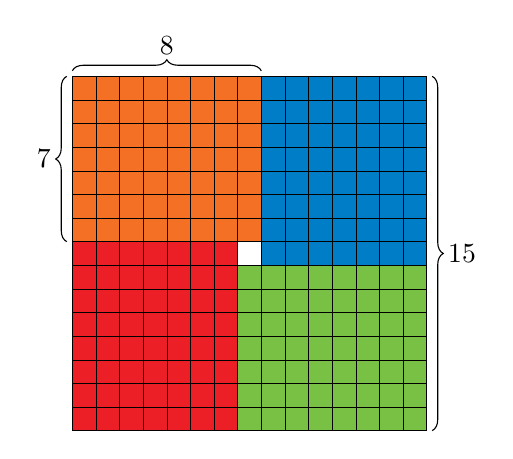
\begin{tikzpicture}[scale=0.30]
            \draw (0, 0) rectangle (15, 15);
            \filldraw[fill=custom-red, draw=black] (0, 0) rectangle (7, 8);
            \filldraw[fill=custom-green, draw=black] (7, 0) rectangle (15, 7);
            \filldraw[fill=custom-blue, draw=black] (8, 7) rectangle (15, 15);
            \filldraw[fill=custom-orange, draw=black] (0, 8) rectangle (8, 15);
            \draw[decorate,decoration={brace, raise=2, amplitude=4}] (0, 8)  -- node[midway, left=0.15]{$7$} (0, 15);
            \draw[decorate,decoration={brace, raise=2, amplitude=4}] (0, 15)  -- node[midway, above=0.15]{$8$} (8, 15);
            \draw[decorate,decoration={brace, raise=2, amplitude=4, mirror}] (15, 0)  -- node[midway, right=0.15]{$15$} (15, 15);
            \draw[very thin] (0, 0) grid (15, 15);
        \end{tikzpicture}
    \caption{Packing of four $7$-by-$8$ rectangles inside a $15$-by-$15$ square.}
    \label{fig:2d-concrete-packing}
\end{figure}

We can generalize this problem. Let $x$ and $y$ be two positive real numbers. Is it possible to pack four $x$-by-$y$ rectangles inside a square whose sides have a length of $x + y$? The area of each rectangle is $xy$, while the area of the square is $(x + y)^2$. We will certainly not be able to fit the rectangles if their combined area exceeds the area of the square. Thus, we do not stand a chance unless $4xy \leq (x + y)^2$. Fortunately, there is still a chance of finding a packing, since $0 \leq (x - y)^2 = (x + y)^2 - 4xy$.
Inspired by \cref{fig:2d-concrete-packing}, we can solve this generalized problem as well. Figure \ref{fig:universal-packing-2d} shows how to pack the four rectangles inside the square, depending of the relative sizes of $x$ and $y$.

\begin{figure}[ht]
    \centering
    \begin{subfigure}[b]{0.3\textwidth}
        \centering
            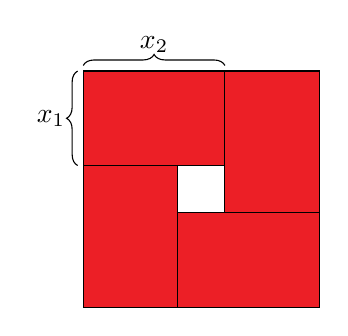
\begin{tikzpicture}[scale=0.60]
                \draw (0, 0) rectangle (5, 5);
                \filldraw[fill=custom-red, draw=black] (0, 0) rectangle (2, 3);
                \filldraw[fill=custom-red, draw=black] (2, 0) rectangle (5, 2);
                \filldraw[fill=custom-red, draw=black] (3, 2) rectangle (5, 5);
                \filldraw[fill=custom-red, draw=black] (0, 3) rectangle (3, 5);
                \draw[decorate,decoration={brace, raise=2pt, amplitude=4pt}] (0, 3)  -- node[midway, left=3pt]{$x_1$} (0, 5);
                \draw[decorate,decoration={brace, raise=2pt, amplitude=4pt}] (0, 5)  -- node[midway, above=3pt]{$x_2$} (3, 5);
            \end{tikzpicture}
        \caption{$x_1 < x_2$}
    \end{subfigure}
    ~
    \begin{subfigure}[b]{0.3\textwidth}
        \centering
            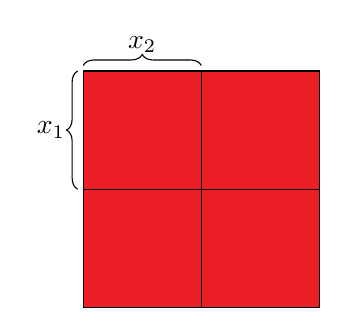
\begin{tikzpicture}[scale=0.60]
                \draw (0, 0) rectangle (5, 5);
                \filldraw[fill=custom-red, draw=black] (0, 0) rectangle (2.5, 2.5);
                \filldraw[fill=custom-red, draw=black] (2.5, 0) rectangle (5, 2.5);
                \filldraw[fill=custom-red, draw=black] (2.5, 2.5) rectangle (5, 5);
                \filldraw[fill=custom-red, draw=black] (0, 2.5) rectangle (2.5, 5);
                \draw[decorate,decoration={brace, raise=2pt, amplitude=4pt}] (0, 2.5)  -- node[midway, left=3pt]{$x_1$} (0, 5);
                \draw[decorate,decoration={brace, raise=2pt, amplitude=4pt}] (0, 5)  -- node[midway, above=3pt]{$x_2$} (2.5, 5);
            \end{tikzpicture}
        \caption{$x_1 = x_2$}
        \label{fig:2d-packing-squares}
    \end{subfigure}
    ~
    \begin{subfigure}[b]{0.3\textwidth}
        \centering
            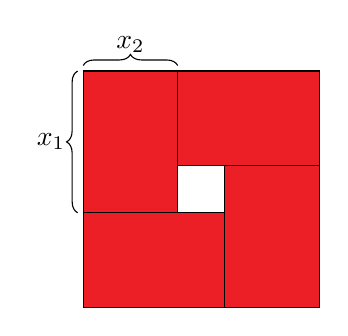
\begin{tikzpicture}[scale=0.60]
                \draw (0, 0) rectangle (5, 5);
                \filldraw[fill=custom-red, draw=black] (0, 0) rectangle (3, 2);
                \filldraw[fill=custom-red, draw=black] (3, 0) rectangle (5, 3);
                \filldraw[fill=custom-red, draw=black] (2, 3) rectangle (5, 5);
                \filldraw[fill=custom-red, draw=black] (0, 2) rectangle (2, 5);
                \draw[decorate,decoration={brace, raise=2pt, amplitude=4pt}] (0, 2)  -- node[midway, left=3pt]{$x_1$} (0, 5);
                \draw[decorate,decoration={brace, raise=2pt, amplitude=4pt}] (0, 5)  -- node[midway, above=3pt]{$x_2$} (2, 5);
            \end{tikzpicture}
        \caption{$x_1 > x_2$}
    \end{subfigure}
    \caption{Solution to the two-dimensional packing problem.}
    \label{fig:universal-packing-2d}
\end{figure}
There is an elegant way to generalize this packing problem to higher dimensions. It is based on the AM-GM inequality, which states that for any $n$ non-negative real numbers $x_1, x_2, \dotsc, x_n$, then
\begin{equation}\label{eq:am-gm-ineq}
\sqrt[n]{x_1 \cdot x_2 \dotsm x_n} \leq \frac{x_1 + x_2 + \dotsb + x_n}{n}
\end{equation}
with equality if and only if $x_1 = x_2 = \dotsb = x_n$. The left-hand side is called the \textit{geometric mean}\index{Geometric mean} while the right-hand side is the familiar \textit{arithmetic mean}\index{Arithmetic mean}. We can turn this inequality into a packing problem by multiplying both sides by $n$, and then raising both sides to the power of $n$. This yields
\[
n^n \paren{x_1 \cdot x_2 \dotsm x_n} \leq \paren{x_1 + x_2 + \dotsb + x_n}^n.
\]
Observe that $x_1 \cdot x_2 \dotsm x_n$ is the hypervolume of an $n$-dimensional hyperrectangle with dimensions $x_1 \times x_2 \times \dotsb \times x_n$ and that $\paren{x_1 + x_2 + \dotsb + x_n}^n$ is the hypervolume of an $n$-dimensional hypercube whose sides have length $x_1 + x_2 + \dotsb + x_n$. So, is it always possible to pack $n^n$ such hyperrectangles inside the $n$-dimensional hypercube? We say that a dimension is \textit{good}\index{Good dimension} if the answer to this question is yes. The above inequality does not guarantee that the hyperrectangles will fit, but only that their combined hypervolume will not exceed the hypervolume of the hypercube.

We have just seen that 2 is a good dimension and in fact so is 3. In the three-dimensional case there are $3^3 = 27$ bricks and \cref{fig:universal-packing-3d} gives a general recipe for constructing a packing. There are in fact 21 such recipes if we ignore reflections and/or rotations.

\begin{figure}[ht]
    \centering
    \begin{subfigure}[b]{0.3\textwidth}
        \centering
            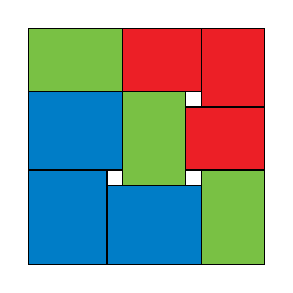
\begin{tikzpicture}[scale=0.2]
                \filldraw[fill=custom-blue, draw=black] (0,0) rectangle (5,6);
\filldraw[fill=custom-blue, draw=black] (0,6) rectangle (6,11);
\filldraw[fill=custom-green, draw=black] (0,11) rectangle (6,15);
\filldraw[fill=custom-blue, draw=black] (5,0) rectangle (11,5);
\filldraw[fill=custom-green, draw=black] (6,5) rectangle (10,11);
\filldraw[fill=custom-red, draw=black] (6,11) rectangle (11,15);
\filldraw[fill=custom-green, draw=black] (11,0) rectangle (15,6);
\filldraw[fill=custom-red, draw=black] (10,6) rectangle (15,10);
\filldraw[fill=custom-red, draw=black] (11,10) rectangle (15,15);
            \end{tikzpicture}
        \caption{Bottom square.}
        \label{fig:3d-special-square}
    \end{subfigure}
    ~
    \begin{subfigure}[b]{0.3\textwidth}
        \centering
            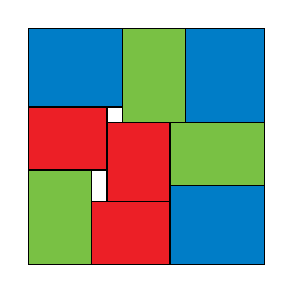
\begin{tikzpicture}[scale=0.2]
                \filldraw[fill=custom-green, draw=black] (0,0) rectangle (4,6);
\filldraw[fill=custom-red, draw=black] (0,6) rectangle (5,10);
\filldraw[fill=custom-blue, draw=black] (0,10) rectangle (6,15);
\filldraw[fill=custom-red, draw=black] (4,0) rectangle (9,4);
\filldraw[fill=custom-red, draw=black] (5,4) rectangle (9,9);
\filldraw[fill=custom-green, draw=black] (6,9) rectangle (10,15);
\filldraw[fill=custom-blue, draw=black] (9,0) rectangle (15,5);
\filldraw[fill=custom-green, draw=black] (9,5) rectangle (15,9);
\filldraw[fill=custom-blue, draw=black] (10,9) rectangle (15,15);
            \end{tikzpicture}
        \caption{Middle square.}
    \end{subfigure}
    ~
    \begin{subfigure}[b]{0.3\textwidth}
        \centering
            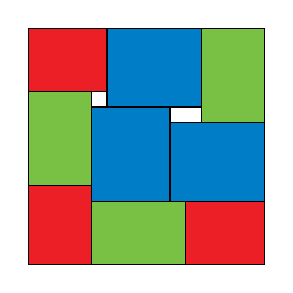
\begin{tikzpicture}[scale=0.2]
                \filldraw[fill=custom-red, draw=black] (0,0) rectangle (4,5);
\filldraw[fill=custom-green, draw=black] (0,5) rectangle (4,11);
\filldraw[fill=custom-red, draw=black] (0,11) rectangle (5,15);
\filldraw[fill=custom-green, draw=black] (4,0) rectangle (10,4);
\filldraw[fill=custom-blue, draw=black] (4,4) rectangle (9,10);
\filldraw[fill=custom-blue, draw=black] (5,10) rectangle (11,15);
\filldraw[fill=custom-red, draw=black] (10,0) rectangle (15,4);
\filldraw[fill=custom-blue, draw=black] (9,4) rectangle (15,9);
\filldraw[fill=custom-green, draw=black] (11,9) rectangle (15,15);
            \end{tikzpicture}
        \caption{Top square.}
    \end{subfigure}
    \caption{Solution to the three-dimensional packing problem. Let $\paren{x_1, x_2, x_3}$ be a dimension tuple with $x_1 \leq x_2 \leq x_3$. Then the $x_1$-by-$x_2$, $x_1$-by-$x_3$ and $x_2$-by-$x_3$ faces are colored red, green and blue, respectively.}
    \label{fig:universal-packing-3d}
\end{figure}

What about higher dimensions? This packing problem has the extraordinary property that if $m$ and $n$ are good dimensions, then $mn$ is good as well. Hence, 4 is a good dimension. It is unknown whether 5 is a good dimension.

The aim of this thesis is to cast light on some of the most interesting unanswered questions of Hoffman's multi\-dimensional packing problem, namely how many packings there are in the four-dimensional case and whether 5 is a good dimension. With the ambition of increasing our knowledge of this problem, we will use experimental mathematics to investigate it.

Experimental mathematics as described in \cite[p. 5-6]{eilers_johansen_2017} is inspired by the methodology of the fields of science where experiments play an essential role in obtaining knowledge. While no amount of experimental data can prove a hypothesis as a mathematical truth (unless it has finitely many cases which can be checked one at a time), it can still play a significant role in guiding the research process.

An experimental approach might provide valuable insights into a mathematical problem---insights which can help us put forward conjectures, find counterexamples and gain an understanding, which may ultimately help us formulate a proof. There is a close interplay with theoretical investigations since, in this way, we can examine the implications of our findings, refine our hypotheses and subsequently conduct more experiments. These experiments could, in theory, be carried out by hand. However, the rapidly growing capabilities of modern computers enable us to perform much more complicated and computationally demanding experiments, which might not previously have been practically feasible to carry out. This continuous expansion of the practical possibilities of experimental mathematics only makes the approach more appealing and promising.

Thanks to Dean G. Hoffman for providing important insights into the inner workings of this packing problem and thanks to Trine K. Boomsma for helping approach the problem using mixed-integer programming and constraint satisfaction.

The repository containing most of the code developed during this project is available at \url{https://github.com/nikolajholck/hoffman}.

\section{Problem formulation and analysis}
\noindent We would like to formalize the formulation of Hoffman's multidimensional packing problem. Let $n$ be a positive integer denoting the dimension of the problem. We will refer to an element $d$ of $(0, \infty)^n$ as an $n$-dimensional \textit{dimension tuple}\index{Dimension tuple} and we refer to the sum of its coordinates as the sum of the dimension tuple\index{Dimension tuple!sum of}. Note that we will typically omit the ``$n$-dimensional'' part of notions, whenever it is clear from the context and for instance simply write ``dimension tuple''.

\begin{definition}[Hyperrectangle]\index{Hyperrectangle}
A subset $R$ of $\R^n$ is an $n$-dimensional \textit{hyperrectangle}, if it can be written as a Cartesian product of $n$ non-empty, open and bounded intervals $I_1, I_2, \dotsc, I_n$ of $\R$, that is $R = I_1 \times I_2 \times \dotsb \times I_n$.
\end{definition}

\noindent In addition, for each $i = 1, 2, \dotsc, n$ let $a_i$ and $b_i$ denote the left and right endpoints of the interval $I_i = (a_i, b_i)$, let $x_i = b_i - a_i$ denote the interval width and let $m_i = (a_i + b_i)/2$ denote the interval midpoint. We will refer to the point $\paren{a_1, a_2, \dotsc, a_n}$ as the \textit{anchor point}\index{Hyperrectangle!anchor point of} and the point $\paren{m_1, m_2, \dotsc, m_n}$ as the \textit{centre}\index{Hyperrectangle!centre of} of the hyperrectangle $R$. We will refer to the tuple $\paren{x_1, x_2, \dotsc, x_n}$ as the dimension tuple of the hyperrectangle\index{Hyperrectangle!dimension tuple of} $R$ and refer to its $i$'th element as the \textit{extent}\index{Hyperrectangle!extend of} of the hyperrectangle along the $i$'th dimension. Lastly, the $n$-dimensional \textit{hypervolume}\index{Hyperrectangle!hypervolume of} of the hyperrectangle $R$ is the product $x_1 x_2 \dotsm x_n$.

Notice that the hyperrectangle $R$ is uniquely identified by its anchor point and dimension tuple, since this information determines the endpoints of $I_i$ for each $i = 1, 2, \dotsc, n$. When we are not interested in the ``position'' of a hyperrectangle in $\R^n$, we will typically just refer to it by its dimension tuple.

\begin{definition}[Hypercube]\index{Hypercube}
An $n$-dimensional \textit{hypercube} is an $n$-dimensional hyperrectangle with the same extent along all dimensions, i.e.\ $x_1 = x_2 = \dotsb = x_n$.
\end{definition}

\begin{definition}[General hyperrectangle]\index{Hyperrectangle!general}
A subset of $\R^n$ is an $n$-dimensional \textit{general hyperrectangle} if it can be rotated into an $n$-dimensional hyperrectangle.
\end{definition}

\noindent Two general hyperrectangles are said to be \textit{overlapping}\index{Hyperrectangle!overlapping} if they intersect one another and \textit{non-overlapping}\index{Hyperrectangle!non-overlapping} if they are disjoint.

\begin{definition}[Packing]\label[definition]{def:general-packing}\index{Packing}
Let $d$ be an $n$-dimensional dimension tuple and let $s$ denote its sum. Suppose $C$ is an $n$-dimensional hypercube with extent $s$, and suppose $B$ is a set of $n$-dimensional general hyperrectangles of $\R^n$, all of which can be rotated into an $n$-dimensional hyperrectangle with dimension tuple $d$. Then $\paren{B, C}$ is a \textit{packing} of $d$, if
\begin{enumerate}[(i)]
  \item The general hyperrectangles in $B$ are pairwise non-overlapping.
  \item Each general hyperrectangle in $B$ is contained in $C$.
\end{enumerate}
\end{definition}

\noindent We will refer to $C$ as the \textit{surrounding}\index{Hypercube!surrounding} hypercube. Note that we can always translate the general hyperrectangles in $B$ and the surrounding hypercube $C$ of a packing $(B, C)$, so that the surrounding hypercube has its centre at the origin of the coordinate system. From now on we will assume that such a translation has been performed, unless otherwise stated. We are now ready to formulate the $n$-dimensional packing problem.

\begin{definition}[Good dimension]
A positive integer $n$ is a good dimension, if for any choice of $n$-dimensional dimension tuple $d$ there exists a packing of $d$.
\end{definition}

\noindent Hoffman asks the following question in \cite[p. 222]{Hoffman1981}, which according to \cite[p. 914]{berlekamp_conway_guy_2004} and recent correspondences with Dean G. Hoffman \cite{hoffman_private} does not appear to have been answered for all dimensions.

\begin{question}
For which positive integers $n$, is $n$ a good dimension?
\end{question}

\noindent \cref{fig:universal-packing-2d} demonstrates that $2$ is a good dimension by showing how to construct a packing of any two-dimensional dimension tuple. According to \cite[p. 215]{Hoffman1981} $3$ is good, but Hoffman does not provide a thorough proof. We provide the first thorough proof of this in \cref{thm:three-is-good}. \cref{thm:multiplication-of-packings} below shows that this packing problem exhibits an extraordinary property, which in particular implies that the number of good dimensions is unbounded. The first appearance of this result is unclear, but Hoffman attributes it to Raphael Robinson in \cite[p. 223]{Hoffman1981}, while Elwyn R. Berlekamp et al. \cite[p. 914]{berlekamp_conway_guy_2004} attribute it to David Seal as well. The proof is based on the one presented by Hoffman in \cite[p. 223--225]{Hoffman1981}.

\FloatBarrier
\begin{theorem}\label[theorem]{thm:multiplication-of-packings}
Suppose $m$ and $n$ are positive integers. If both $m$ and $n$ are good dimensions, then $mn$ is a good dimension as well.
\end{theorem}
\begin{proof}
Suppose $m$ and $n$ are good dimensions and let
\[
\paren{
x_{1, 1}, x_{1, 2}, \dotsc, x_{1, n},
x_{2, 1}, x_{2, 2}, \dotsc, x_{2, n},
\dotsc,
x_{m, 1}, x_{m, 2}, \dotsc, x_{m, n}
}
\]
be an $mn$-dimensional dimension tuple and let $t$ denote its sum. We would like to show that there exists a packing of this dimension tuple. Suppose we have $(mn)^{mn}$ $mn$-dimensional hyperrectangles with the above dimension tuple. We would like to rotate and translate them to fit inside an $mn$-dimensional hypercube with an extent of $t$. For the sake of readability we will write out the dimension tuple in an $m \times n$ matrix
\[
A = \begin{pmatrix}
x_{1, 1} & x_{1, 2} & \cdots & x_{1, n} \\
x_{2, 1} & x_{2, 2} & \cdots & x_{2, n} \\
\vdots   & \vdots   & \ddots & \vdots   \\
x_{m, 1} & x_{m, 2} & \cdots & x_{m, n}
\end{pmatrix}.
\]
Let $s_i$ be the sum of the $i$'th column of $A$ for $i = 1, 2, \dotsc, n$. First, divide the $(mn)^{mn}$ $mn$-dimensional hyperrectangles into groups, each consisting of $m^m$ hyperrectangles. There must be $(mn)^{mn}/m^m = m^{m(n-1)}n^{mn}$ of these groups. Consider the dimension tuple $\paren{x_{1, 1}, x_{2, 1}, \dotsc, x_{m, 1}}$ consisting of the first column of $A$ and recall that its sum is $s_1$. Since $m$ is a good dimension, there exists a packing of $m^m$ $m$-dimensional general hyperrectangles (which can be rotated to have this dimension tuple) inside an $m$-dimensional hypercube with an extent of $s_1$. Then we see that the $m^m$ $mn$-dimensional hyperrectangles in each group will fit inside an $mn$-dimensional hyperrectangle with dimension tuple (as a matrix)
\[
\begin{pmatrix}
s_1    & x_{1, 2} & \cdots & x_{1, n} \\
s_1    & x_{2, 2} & \cdots & x_{2, n} \\
\vdots & \vdots   & \ddots & \vdots   \\
s_1    & x_{m, 2} & \cdots & x_{m, n}
\end{pmatrix}.
\]
By ``fit'' we mean that the $m^m$ hyperrectangles are pairwise non-overlapping and rotated and translated such that they are subsets of the surrounding hyperrectangle like in \cref{def:general-packing}. Doing this for each group results in $m^{m(n-1)}n^{mn}$ such $mn$-dimensional hyperrectangles---each containing $m^m$ of the original $mn$-dimensional hyperrectangles, rotated and translated appropriately. We repeat this procedure for every column, each time dividing the $mn$-dimensional hyperrectangles constructed at the previous iteration into groups with a size of $m^m$ and then fitting the hyperrectangles of each group into a surrounding $mn$-dimensional hyperrectangle. After doing this a total number of $n$ times, we end up with $n^{mn}$ groups of $mn$-dimensional hyperrectangles each of which fits inside an $mn$-dimensional hyperrectangle with dimension tuple (as a matrix)
\[
B = \begin{pmatrix}
s_1    & s_2    & \cdots & s_n    \\
s_1    & s_2    & \cdots & s_n    \\
\vdots & \vdots & \ddots & \vdots \\
s_1    & s_2    & \cdots & s_n
\end{pmatrix}.
\]
Each of these $mn$-dimensional hyperrectangles contains $m^{mn}$ of the original $mn$-dimensional hyperrectangles, rotated and translated appropriately. Next, we perform a similar procedure for each row. We divide the $n^{mn}$ $mn$-dimensional hyperrectangles into groups of $n^n$ hyperrectangles. There are $n^{mn}/n^n = n^{(m - 1)n}$ of these groups. Consider the dimension tuple $\paren{s_1, s_2, \dotsc, s_n}$ consisting of the first row of $B$ and notice that the sum along this row is $t$. Since $n$ is a good dimension, there exists a packing of $n^n$ $n$-dimensional general hyperrectangles (which can be rotated to have this dimension tuple) inside an $n$-dimensional hypercube with an extent of $t$. Then the $n^n$ $mn$-dimensional hyperrectangles in each group will fit inside an $mn$-dimensional hyperrectangle with dimension tuple (as a matrix)
\[
\begin{pmatrix}
t      & t      & \cdots & t      \\
s_1    & s_2    & \cdots & s_n    \\
\vdots & \vdots & \ddots & \vdots \\
s_1    & s_2    & \cdots & s_n
\end{pmatrix}.
\]
Doing so for each group, we obtain $n^{(m - 1)n}$ such $mn$-dimensional hyperrectangles---each containing $m^{mn} n^n$ of the original $mn$-dimensional hyperrectangles, rotated and translated appropriately. Repeating this procedure for each row, $m$ times in total, we end up with $n^{(m - m)n} = 1$ group of $n^n$ $mn$-dimensional hyperrectangles fitting inside an $mn$-dimensional hyperrectangle with dimension tuple (as a matrix)
\[
\begin{pmatrix}
t      & t      & \cdots & t      \\
t      & t      & \cdots & t      \\
\vdots & \vdots & \ddots & \vdots \\
t      & t      & \cdots & t
\end{pmatrix}.
\]
This is in fact an $mn$-dimensional hypercube with an extent of $t$ and the desired packing is obtained by repeatedly unwrapping the groups of rotated and translated $mn$-dimensional hyperrectangles, until we reach the now appropriately rotated and translated $(mn)^{mn}$ $mn$-dimensional hyperrectangles.
\end{proof}

\noindent It follows from this result that in order to prove that all dimensions are good, one would only have to prove so for all prime numbers. Hence, 4 is a good dimension, and in the light of \cref{thm:three-is-good} the smallest unsettled dimension is 5 \cite[p. 223]{Hoffman1981}\cite[p. 914]{berlekamp_conway_guy_2004}.

If $n$ is a good dimension, it is natural to ask how many different packings there are in that particular dimension. Before we can even attempt to answer this question, we need to make sure that the number of different packings is independent of the choice of dimension tuple. This will ultimately lead to the definition of a universal packing and a refinement of the question. In preparation for this, we will first need a notion of two packings being notably different.

\subsection{Equivalence of packings}
Depending on the choice of dimension tuple $d$ there might be enough unoccupied ``room'' inside the surrounding hypercube to rearrange the general hyperrectangles without intersecting one another and without leaving the surrounding hypercube.

\begin{definition}[Rearrangement]\index{Packing!rearrangement of}
Suppose $(B_1, C_1)$ and $(B_2, C_2)$ are packings of the dimension tuples $d_1$ and $d_2$, respectively. The first packing is a \textit{rearrangement} of the second if $C_1$ coincides with $C_2$ and if it is possible to continuously move (using only translations and rotations) the general hyperrectangles in $B_1$, so that each moved general hyperrectangle coincides with a general hyperrectangle in $B_2$ without breaking any of the criteria in \cref{def:general-packing} while moving.
\end{definition}

\begin{figure}[h]
    \centering
    \begin{subfigure}[b]{0.37\textwidth}
        \centering
            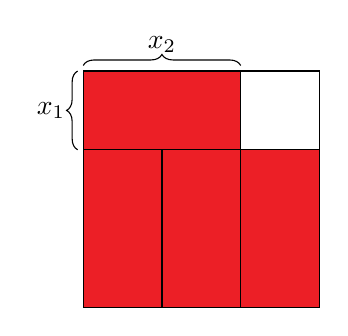
\begin{tikzpicture}[scale=0.60*5/3]
                \draw (0, 0) rectangle (3, 3);
                \filldraw[fill=custom-red, draw=black] (0, 0) rectangle (1, 2);
                \filldraw[fill=custom-red, draw=black] (1, 0) rectangle (2, 2);
                \filldraw[fill=custom-red, draw=black] (2, 0) rectangle (3, 2);
                \filldraw[fill=custom-red, draw=black] (0, 2) rectangle (2, 3);
                \draw[decorate,decoration={brace, raise=2pt, amplitude=4pt}] (0, 2)  -- node[midway, left=3pt]{$x_1$} (0, 3);
                \draw[decorate,decoration={brace, raise=2pt, amplitude=4pt}] (0, 3)  -- node[midway, above=3pt]{$x_2$} (2, 3);
            \end{tikzpicture}
        \caption{Packing with three rectangles side by side.}
        \label{fig:extreme-packing-2d}
    \end{subfigure}
    ~
    \begin{subfigure}[b]{0.37\textwidth}
        \centering
            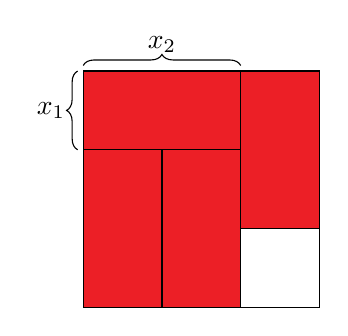
\begin{tikzpicture}[scale=0.60*5/3]
                \draw (0, 0) rectangle (3, 3);
                \filldraw[fill=custom-red, draw=black] (0, 0) rectangle (1, 2);
                \filldraw[fill=custom-red, draw=black] (1, 0) rectangle (2, 2);
                \filldraw[fill=custom-red, draw=black] (2, 1) rectangle (3, 3);
                \filldraw[fill=custom-red, draw=black] (0, 2) rectangle (2, 3);
                \draw[decorate,decoration={brace, raise=2pt, amplitude=4pt}] (0, 2)  -- node[midway, left=3pt]{$x_1$} (0, 3);
                \draw[decorate,decoration={brace, raise=2pt, amplitude=4pt}] (0, 3)  -- node[midway, above=3pt]{$x_2$} (2, 3);
            \end{tikzpicture}
        \caption{Rearrangement of the packing in Figure \ref{fig:extreme-packing-2d}.}
        \label{fig:rearrangement-packing-2d}
    \end{subfigure}
    \caption{Example of equivalent two-dimensional packings of the dimension tuple $\paren{x_1, x_2}$ where $x_2 = 2 x_1$.}
\end{figure}

\noindent It is also natural to take reflections and rotations of the packing as a whole into account. We can view such a transformation as a linear map represented by an orthogonal $n \times n$ matrix. There are an infinite number of these, but by \cref{def:general-packing} we only have to consider those mapping the surrounding hypercube to itself. This corresponds to the linear maps sending the standard basis vectors $e_1, e_2, \dotsc, e_n$ to some permutation of themselves while possibly changing the sign of some of them. Thus, there are $n! \cdot 2^n$ reflections and/or rotations of an $n$-dimensional hypercube. We will refer to reflections and/or rotations as \textit{symmetries}\index{Packing!symmetry of}. With this in mind, we will define what it means for two packings to be equivalent.

\begin{definition}[Equivalent packings]\index{Packing!equivalence of}
Suppose there are two packings of the dimension tuples $d_1$ and $d_2$, respectively. These packings are \textit{equivalent} if there exists a rearrangement of the first packing coinciding with a symmetry of the second.
\end{definition}

\noindent This is an equivalence relation and we will refer to the equivalence classes as unique packings. Notice that it is possible to permute the elements in a dimension tuple without influencing the number of unique packings, since such a permutation corresponds to rotating all packings and thus does not affect the equivalence classes. We can therefore without loss of generality restrict ourselves to increasing dimension tuples. We say that a dimension tuple $d = \paren{x_1, x_2, \dotsc, x_n}$ is \textit{increasing}\index{Dimension tuple!increasing} if $x_1 \leq x_2 \leq \dotsb \leq x_n$.

The notion of rearrangements of a packing also gives rise to defining a rigid packing, that is a packing where all the general hyperrectangles are ``locked into place'' by the surrounding general hyperrectangles or hypercube.

\begin{definition}[Rigid packing]\index{Packing!rigid}
We say that a packing is \textit{rigid} if all of its rearrangements are identical to itself.
\end{definition}

\noindent \cref{fig:universal-packing-2d} is an example of a rigid packing. Note that the equivalence class of a rigid packing only contains its symmetries, so it contains at most $n! \cdot 2^n$ packings. It might contain fewer if some symmetries are identical to one another.

Next, we will examine packings of dimension tuples satisfying a certain inequality, which forces any packing consisting of hyperrectangles to be rigid and ultimately leads to the definition of a universal packing.

\subsection{Universal packings} Before defining a universal packing, it is helpful to get some intuition by looking a bit closer at the two-dimensional packing problem. Consider some increasing dimension tuple $\paren{x_1, x_2}$. There are ways of organizing the four rectangles, which are only possible when the relative difference between $x_1$ and $x_2$ is sufficiently large. Suppose $x_2$ is twice as large as $x_1$, i.e.\ $x_2 = 2x_1$ or equivalently $x_1 + x_2 = 3 x_1$. Then the packing in Figure \ref{fig:extreme-packing-2d} becomes possible. This packing is only feasible because we can fit three rectangles side by side. It turns out that restricting the search to packings of increasing dimension tuples satisfying the inequality
\begin{equation}\label{eq:ineq-2d}
x_1 + x_2 < 3x_1
\end{equation}
prevents this and restricts the problem in an interesting way. Later, we will argue that any packing of an increasing dimension tuple satisfying \eqref{eq:ineq-2d} consisting of hyperrectangles will be rigid and discuss whether it gives a ``recipe'' for constructing a packing of \textit{any} dimension tuple as seen in \cref{fig:universal-packing-2d}. Thus, it is possible to reuse the same ``universal packing'' even for dimension tuples not satisfying \eqref{eq:ineq-2d}. This is the inspiration behind our future definition of a ``universal packing''.

Notice that the packing in \cref{fig:extreme-packing-2d}---which relied on \eqref{eq:ineq-2d} not being satisfied---is not rigid. Intuitively, \eqref{eq:ineq-2d} ensures that the four rectangles resemble a square to such a degree that any packing must necessarily resemble the packing \cref{fig:2d-packing-squares}, where four squares are neatly organized in a grid inside the surrounding square. We will return to this concept of a grid shortly. The inequality \eqref{eq:ineq-2d} is inspired by Hoffman who proposed a three-dimensional version of it in \cite[p. 215]{Hoffman1981}, namely
\begin{equation}\label{eq:ineq-3d}
x_1 + x_2 + x_3 < 4x_1.
\end{equation}
Therefore we will name it after Hoffman when we generalize it to $n$ dimensions.

\begin{definition}[Hoffman's inequality]\index{Hoffman's inequality}
A dimension tuple $\paren{x_1, x_2, \dotsc, x_n}$ satisfies \textit{Hoffman's inequality} if it is increasing and
\[
x_1 + x_2 + \dotsb + x_n < (n + 1)x_1.
\]
\end{definition}

\noindent Choosing $x_1 = x_2 = \dotsb = x_n$ for some positive real number shows that a dimension tuple with this property exists in all dimensions. Notice that \eqref{eq:ineq-2d} and \eqref{eq:ineq-3d} are really Hoffman's inequality for $n = 2$ and $n = 3$, respectively. Intuitively, Hoffman's inequality ensures that no packing can contain $n + 1$ or more hyperrectangles side by side. Shortly, we will justify that packings (consisting solely of hyperrectangles) of a dimension tuple satisfying Hoffman's inequality must be rigid and prove that the hyperrectangles must be arranged in a ``grid''.

Hoffman restricts his search for three-dimensional packings in \cite[p. 215]{Hoffman1981} to dimension tuples satisfying Hoffman's inequality for $n = 3$, that is \eqref{eq:ineq-3d}. George Miller \cite{Miller_2006} credits Donald Knuth for searching for three-dimensional packings of the dimension tuple $\paren{3, 4, 5}$ and discovering solutions where one could squeeze an additional 28th 3-dimensional hyperrectangle (brick) into the surrounding cube (which has an extent of $3 + 4 + 5 = 12$).
\begin{figure}[ht]
    \centering
    \begin{subfigure}[b]{0.8\textwidth}
        \centering
            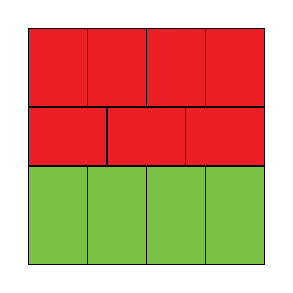
\begin{tikzpicture}[scale=0.2*15/12]
            \filldraw[fill=custom-green, draw=black] (0,0) rectangle (3,5);
\filldraw[fill=custom-green, draw=black] (3,0) rectangle (6,5);
\filldraw[fill=custom-green, draw=black] (6,0) rectangle (9,5);
\filldraw[fill=custom-green, draw=black] (9,0) rectangle (12,5);

\filldraw[fill=custom-red, draw=black] (0,5) rectangle (4,9);
\filldraw[fill=custom-red, draw=black] (4,5) rectangle (8,9);
\filldraw[fill=custom-red, draw=black] (8,5) rectangle (12,9);

\filldraw[fill=custom-red, draw=black] (0,8) rectangle (3,12);
\filldraw[fill=custom-red, draw=black] (3,8) rectangle (6,12);
\filldraw[fill=custom-red, draw=black] (6,8) rectangle (9,12);
\filldraw[fill=custom-red, draw=black] (9,8) rectangle (12,12);

            \end{tikzpicture}
            \hfill
            
\begin{tikzpicture}[scale=0.2*15/12]
            \draw (0,0) rectangle (12,12);

\filldraw[fill=custom-blue, draw=black] (0,0) rectangle (4,5);
\filldraw[fill=custom-blue, draw=black] (4,0) rectangle (8,5);
\filldraw[fill=custom-blue, draw=black] (8,0) rectangle (12,5);

\filldraw[fill=custom-blue, draw=black] (0,7) rectangle (4,12);
\filldraw[fill=custom-blue, draw=black] (4,7) rectangle (8,12);
\filldraw[fill=custom-blue, draw=black] (8,7) rectangle (12,12);

            \end{tikzpicture}
            \hfill
            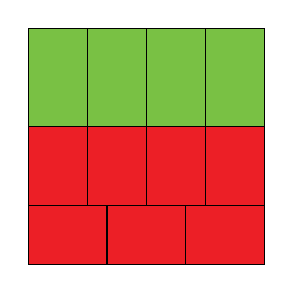
\begin{tikzpicture}[scale=0.2*15/12]
            \filldraw[fill=custom-red, draw=black] (0,0) rectangle (4,4);
\filldraw[fill=custom-red, draw=black] (4,0) rectangle (8,4);
\filldraw[fill=custom-red, draw=black] (8,0) rectangle (12,4);

\filldraw[fill=custom-red, draw=black] (0,3) rectangle (3,7);
\filldraw[fill=custom-red, draw=black] (3,3) rectangle (6,7);
\filldraw[fill=custom-red, draw=black] (6,3) rectangle (9,7);
\filldraw[fill=custom-red, draw=black] (9,3) rectangle (12,7);

\filldraw[fill=custom-green, draw=black] (0,7) rectangle (3,12);
\filldraw[fill=custom-green, draw=black] (3,7) rectangle (6,12);
\filldraw[fill=custom-green, draw=black] (6,7) rectangle (9,12);
\filldraw[fill=custom-green, draw=black] (9,7) rectangle (12,12);

            \end{tikzpicture}
        \caption{Layers of first solution.}
    \end{subfigure}
    \par\bigskip
    \begin{subfigure}[b]{0.8\textwidth}
        \centering
            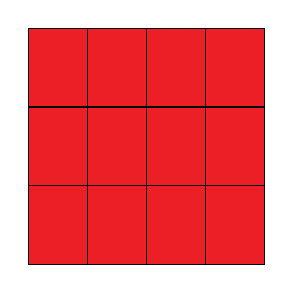
\begin{tikzpicture}[scale=0.2*15/12]
            \filldraw[fill=custom-red, draw=black] (0,8) rectangle (3,12);
\filldraw[fill=custom-red, draw=black] (3,8) rectangle (6,12);
\filldraw[fill=custom-red, draw=black] (6,8) rectangle (9,12);
\filldraw[fill=custom-red, draw=black] (9,8) rectangle (12,12);

\filldraw[fill=custom-red, draw=black] (0,4) rectangle (3,8);
\filldraw[fill=custom-red, draw=black] (3,4) rectangle (6,8);
\filldraw[fill=custom-red, draw=black] (6,4) rectangle (9,8);
\filldraw[fill=custom-red, draw=black] (9,4) rectangle (12,8);

\filldraw[fill=custom-red, draw=black] (0,0) rectangle (3,4);
\filldraw[fill=custom-red, draw=black] (3,0) rectangle (6,4);
\filldraw[fill=custom-red, draw=black] (6,0) rectangle (9,4);
\filldraw[fill=custom-red, draw=black] (9,0) rectangle (12,4);

            \end{tikzpicture}
            \hfill
            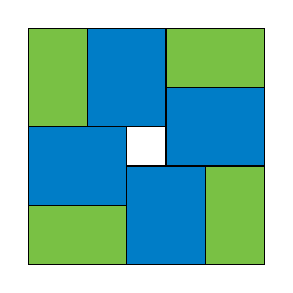
\begin{tikzpicture}[scale=0.2*15/12]
            \filldraw[fill=custom-green, draw=black] (0,0) rectangle (5,3);
\filldraw[fill=custom-blue, draw=black] (5,0) rectangle (9,5);
\filldraw[fill=custom-green, draw=black] (9,0) rectangle (12,5);

\filldraw[fill=custom-blue, draw=black] (0,3) rectangle (5,7);
\filldraw[fill=custom-blue, draw=black] (7,5) rectangle (12,9);

\filldraw[fill=custom-green, draw=black] (0,7) rectangle (3,12);
\filldraw[fill=custom-blue, draw=black] (3,7) rectangle (7,12);
\filldraw[fill=custom-green, draw=black] (7,9) rectangle (12,12);

            \end{tikzpicture}
            \hfill
            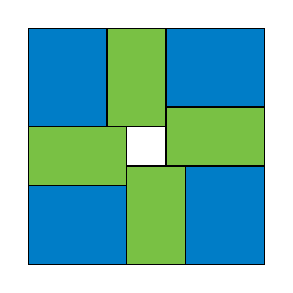
\begin{tikzpicture}[scale=0.2*15/12]
            \filldraw[fill=custom-blue, draw=black] (0,0) rectangle (5,4);
\filldraw[fill=custom-green, draw=black] (5,0) rectangle (8,5);
\filldraw[fill=custom-blue, draw=black] (8,0) rectangle (12,5);

\filldraw[fill=custom-green, draw=black] (0,4) rectangle (5,7);
\filldraw[fill=custom-green, draw=black] (7,5) rectangle (12,8);

\filldraw[fill=custom-blue, draw=black] (0,7) rectangle (4,12);
\filldraw[fill=custom-green, draw=black] (4,7) rectangle (7,12);
\filldraw[fill=custom-blue, draw=black] (7,8) rectangle (12,12);
            \end{tikzpicture}
        \caption{Layers of second solution.}
    \end{subfigure}
    \par\bigskip
    \begin{subfigure}[b]{0.8\textwidth}
        \centering
            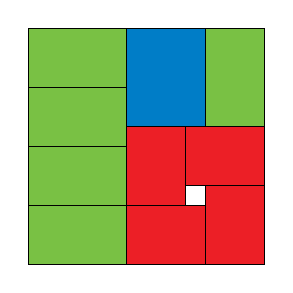
\begin{tikzpicture}[scale=0.2*15/12]
            \filldraw[fill=custom-green, draw=black] (0,0) rectangle (5,3);
\filldraw[fill=custom-green, draw=black] (0,3) rectangle (5,6);
\filldraw[fill=custom-green, draw=black] (0,6) rectangle (5,9);
\filldraw[fill=custom-green, draw=black] (0,9) rectangle (5,12);

\filldraw[fill=custom-red, draw=black] (5,0) rectangle (9,3);
\filldraw[fill=custom-red, draw=black] (9,0) rectangle (12,4);
\filldraw[fill=custom-red, draw=black] (5,3) rectangle (8,7);
\filldraw[fill=custom-red, draw=black] (8,4) rectangle (12,7);

\filldraw[fill=custom-blue, draw=black] (5,7) rectangle (9,12);
\filldraw[fill=custom-green, draw=black] (9,7) rectangle (12,12);

            \end{tikzpicture}
            \hfill
            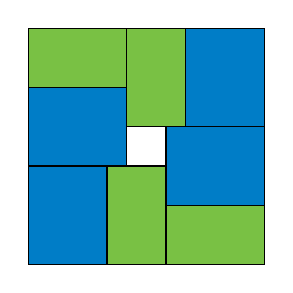
\begin{tikzpicture}[scale=0.2*15/12]
            \filldraw[fill=custom-blue, draw=black] (0,0) rectangle (4,5);
\filldraw[fill=custom-green, draw=black] (4,0) rectangle (7,5);
\filldraw[fill=custom-green, draw=black] (7,0) rectangle (12,3);

\filldraw[fill=custom-blue, draw=black] (0,5) rectangle (5,9);
\filldraw[fill=custom-blue, draw=black] (7,3) rectangle (12,7);

\filldraw[fill=custom-green, draw=black] (0,9) rectangle (5,12);
\filldraw[fill=custom-green, draw=black] (5,7) rectangle (8,12);
\filldraw[fill=custom-blue, draw=black] (8,7) rectangle (12,12);

            \end{tikzpicture}
            \hfill
            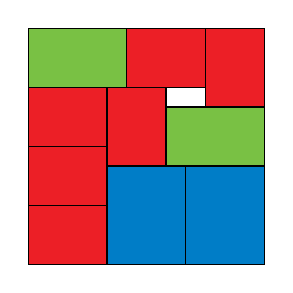
\begin{tikzpicture}[scale=0.2*15/12]
            \filldraw[fill=custom-red, draw=black] (0,0) rectangle (4,3);
\filldraw[fill=custom-red, draw=black] (0,3) rectangle (4,6);
\filldraw[fill=custom-red, draw=black] (0,6) rectangle (4,9);
\filldraw[fill=custom-green, draw=black] (0,9) rectangle (5,12);

\filldraw[fill=custom-blue, draw=black] (4,0) rectangle (8,5);
\filldraw[fill=custom-blue, draw=black] (8,0) rectangle (12,5);

\filldraw[fill=custom-red, draw=black] (4,5) rectangle (7,9);
\filldraw[fill=custom-green, draw=black] (7,5) rectangle (12,8);
\filldraw[fill=custom-red, draw=black] (5,9) rectangle (9,12);
\filldraw[fill=custom-red, draw=black] (9,8) rectangle (12,12);

            \end{tikzpicture}
        \caption{Layers of third solution.}
    \end{subfigure}
    \caption{The three solutions of the dimension tuple $\paren{3, 4, 5}$ consisting of 28 bricks found by Donald Knuth \cite{Knuth_2004}.}
    \label{fig:knuth-solutions-3d}
\end{figure}
Knuth's solutions \cite{Knuth_2004} are presented in \cref{fig:knuth-solutions-3d}. Notice that in each of them it is possible to remove one of the 28 bricks such that the resulting packing of $\paren{3, 4, 5}$ is not rigid and such that the remaining bricks do not seem to be organized in a ``grid''. The attentive reader might have noticed that this particular dimension tuple satisfies $x_1 + x_2 + x_3 = 4x_1$, so it barely breaks with \eqref{eq:ineq-3d}, that is Hoffman's inequality. Thus, Hoffman's inequality might intuitively be interpreted is a boundary separating us from a whole different class of packings, including those with $n + 1$ or more hyperrectangles side by side. For instance all of the solutions in \cite{Knuth_2004} have four bricks side by side somewhere. As seen in \cref{fig:extreme-packing-2d} for $n = 2$, this class of packings can not serve as a ``recipe'' for constructing packings of dimension tuples satisfying Hoffman's inequality. Therefore we will disregard them in our search for a ``universal packing''.

Let us clarify what we mean by a grid. Let $s > 0$ and consider the $n$-dimensional hypercube $S = (0, s)^n$ which has an extent of $s$. Let $c_i = is/(n + 1)$ for $i = 1, 2, \dotsc, n$ and observe that $0 < c_i < s$ and also that $c_{i + 1} - c_i = s/(n + 1)$ for all suitable $i$. Define $s/(n + 1)$ as the \textit{cut distance}\index{cut distance} and define a \textit{cut}\index{cut} at position $k$ along dimension $i$ to be $C_{i, k} = \curly{ v \in \R^n \mid v_i = c_k }$ for $i, k = 1, 2, \dotsc, n$. Intersecting $n$ cuts $C_{i, k_i}$, one along each dimension $i = 1, 2, \dotsc, n$, yields a subset of $\R^n$ containing a single point, namely
\[
\bigcap_{i = 1}^n C_{i, k_i}
= \curly{ v \in \R^n \mid v_1 = c_{k_1}, v_2 = c_{k_2}, \dotsc, v_n = c_{k_n} }
= \curly{\paren{c_{k_1}, c_{k_2}, \dotsc, c_{k_n}}},
\]
and this point is inside the hypercube $S$. Any such intersection corresponds to precisely one point in the subset $\curly{c_1, c_2, \dotsc, c_n}^n$ of the hypercube $S$ and we will refer to this subset as the \textit{grid}\index{Grid} of the hypercube $S$ and to each of its $n^n$ elements as a \textit{grid point}\index{Grid point}. \cref{fig:grid} illustrates this construction in the three-dimensional case. Using translations, it is always possible to construct the grid of a hypercube. This enables us to formulate and prove the next result. The proof is a formalization and generalization of Hoffman's proof of the three-dimensional case in \cite[p. 218--219]{Hoffman1981} and it is therefore only appropriate to name it after him.

\begin{figure}[ht]
    \centering
    \begin{subfigure}[b]{0.3\textwidth}
        \centering
            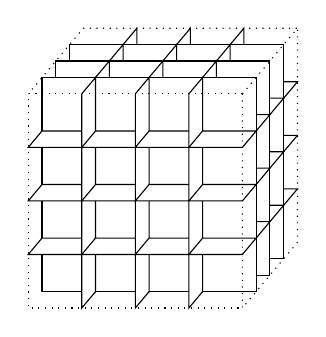
\begin{tikzpicture}[scale=0.68, z={(230:0.4cm)}]
                \foreach \z in {0, ..., 3} {
                    \ifthenelse{\z = 0}{}{
                        \filldraw[fill=white, draw=black] (0, 0, \z) -- ++(4, 0, 0) -- ++(0, 4, 0) -- ++(-4, 0, 0) -- cycle;
                    }
                    \foreach \x in {0, ..., 3} {
                        \ifthenelse{\x = 0}{}{
                            \filldraw[fill=white, draw=black] (\x, 0, \z) -- ++(0, 4, 0) -- ++(0, 0, 1) -- ++(0, -4, 0) -- cycle;
                        }
                        \foreach \y in {1, ..., 3} {
                            \filldraw[fill=white, draw=black] (\x, \y, \z) -- ++(1, 0, 0) -- ++(0, 0, 1) -- ++(-1, 0, 0) -- cycle;
                        }
                    }
                }
                \boxfront{0}{0}{0}{4}{4}{4}{dotted}
            \end{tikzpicture}
        \caption{Cuts.}
    \end{subfigure}
    \hfill
    \begin{subfigure}[b]{0.3\textwidth}
        \centering
            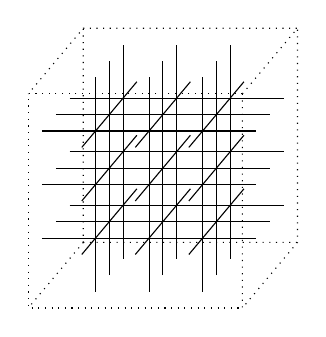
\begin{tikzpicture}[scale=0.68, z={(230:0.4cm)}]
                \boxback{0}{0}{0}{4}{4}{4}{dotted}
                \foreach \a in {1, ..., 3} {
                    \foreach \b in {1, ..., 3} {
                        \draw [black] (\a, \b, 0) -- ++(0, 0, 4);
                        \draw [black] (\a, 0, \b) -- ++(0, 4, 0);
                        \draw [black] (0, \a, \b) -- ++(4, 0, 0);
                    }
                }
                \boxfront{0}{0}{0}{4}{4}{4}{dotted}
            \end{tikzpicture}
        \caption{Grid lines.}
    \end{subfigure}
    \hfill
    \begin{subfigure}[b]{0.3\textwidth}
        \centering
            \begin{tikzpicture}[scale=0.68, z={(230:0.4cm)}]
                \boxback{0}{0}{0}{4}{4}{4}{dotted}
                \foreach \x in {1, ..., 3} {
                    \foreach \y in {1, ..., 3} {
                        \filldraw[black] (\x, 1, \y) circle (1pt);
                        \filldraw[black] (\x, 2, \y) circle (1pt);
                        \filldraw[black] (\x, 3, \y) circle (1pt);
                    }
                }
                \boxfront{0}{0}{0}{4}{4}{4}{dotted}
            \end{tikzpicture}
        \caption{Grid points.}
    \end{subfigure}
    \caption{Example of cuts and the grid of a cube in three dimensions.}
    \label{fig:grid}
\end{figure}

\begin{theorem}[Hoffman's grid theorem]\label[theorem]{thm:grid-theorem}
Suppose $d$ is a dimension tuple satisfying Hoffman's inequality and suppose $(B, C)$ is a packing of $d$ such that $B$ contains solely hyperrectangles. Then each hyperrectangle in $B$ contains exactly one grid point of the grid of $C$.
\end{theorem}

\begin{proof}
Let $d = \paren{x_1, x_2, \dotsc, x_n}$ and $s = x_1 + x_2 + \dotsb + x_n$. Assume without loss of generality that the packing has been translated, so that the anchor point of the surrounding hypercube is at the origin of the coordinate system, i.e.\ $C = (0, s)^n$, whereby we can reuse the grid construction described above.

We first show that every hyperrectangle in $B$ contains a grid point. Take some hyperrectangle $R$ in $B$ and write it as a Cartesian product $R = I_1 \times I_2 \times \dotsb \times I_n$ where each $I_i$ is a non-empty, open and bounded interval of $\R$. Next, pick some dimension $k$ in $\curly{1, 2, \dotsc, n}$. We would like to show that there exists a cut along the dimension $k$ which intersects the hyperrectangle $R$. Let $r_k$ denote the extent of the hyperrectangle $R$ along the $k$'th dimension, i.e.\ the width of the interval $I_k$. Since $(B, C)$ is a packing of $d$ the hyperrectangle $R$ is a subset of the hypercube $C$, whereby $I_k$ must be a subset of $(0, s)$. Notice that each $c_i$ from the grid construction is evenly distributed inside $(0, s)$ and cuts it up into $n + 1$ intervals of width equal to the cut distance $s/(n + 1)$. It then follows from Hoffman's inequality that $s/(n + 1) < x_1 \leq r_k$, so there must exist some $j_k$ in $\curly{1, 2, \dotsc, n}$ such that $c_{j_k}$ is in $I_k$. Then the cut $C_{k, j_k}$ at position $j_k$ along dimension $k$ must intersect the hyperrectangle $R$, since all $I_i$ are non-empty. Repeating this procedure for all dimensions $k$ gives $n$ cuts $C_{k, j_k}$ intersecting the hyperrectangle, one along each dimension. Intersecting these cuts results in a set with a single grid point, in this case $\paren{ c_{j_1}, c_{j_2}, \dotsc, c_{j_n} }$. This point is inside the hyperrectangle $R$, since each $c_{j_k}$ is inside$I_k$. Hence, there is a least one grid point inside each hyperrectangle in $B$.

Lastly, since $(B, C)$ is a packing of $d$, then the hyperrectangles in $B$ are pairwise non-overlapping. Then there can not be more than one grid point inside any of the $n^n$ hyperrectangles in $B$, since there are only $n^n$ grid points in total.
\end{proof}

\noindent Let us introduce a convenient way of working with this grid. Define the $n$-dimen\-sional grid point coordinates $G_n$ to be the set $\curly{1, 2, \dotsc, n}^n$ and note that for any $n$-dimensional hypercube, it is possible to identify each of its grid points through the bijective map from $G_n$ to the grid given by $\paren{p_1, p_2, \dotsc, p_n} \mapsto \paren{c_{p_1}, c_{p_2}, \dotsc, c_{p_n}}$. We will typically refer to a grid point by its coordinates\index{Grid point!coordinate} assigned via this bijection.

We say that two grid point coordinates are on the same \textit{grid line}\index{Grid line} if all but one of their entries match, and we say that this grid line runs along the dimension numbered by the index where the coordinates differ. Note that there are precisely $n$ grid point coordinates on any grid line. For each grid point coordinate $p$ in $G_n$ and each dimension $k = 1, 2, \dotsc, n$ we define $L(p, k, i)$ as the $i$'th grid point coordinate on the line passing through $p$ along dimension $k$ for $i = 1, 2, \dotsc, n$, that is
\[
L(p, k, i)_j =
\begin{cases}
i,   & \text{if } j = k \\
p_j, & \text{if } j \neq k
\end{cases}
\]
for $j = 1, 2, \dotsc, n$ and note that $L(p, k, p_k) = p$ for all $k = 1, 2, \dotsc, n$.

Suppose $d = \paren{x_1, x_2, \dotsc, x_n}$ is a dimension tuple satisfying Hoffman's inequality and suppose $(B, C)$ is a packing of $d$ such that $B$ contains solely hyperrectangles. Let $p$ be a grid point coordinate in $G_n$ and for $i = 1, 2, \dotsc, n$ define $w(p)_i$ as the extent along the $i$'th dimension of the hyperrectangle in $B$ containing this particular grid point. This is well-defined by Hoffman's grid theorem \labelcref{thm:grid-theorem}. We measure the \textit{stuffing}\index{Grid line!stuffing on} on a grid line $L(p, k, i)$ as the sum of the extents along the $k$'th dimension of the hyperrectangles associated with the grid points on the grid line, that is
\[
\sum_{i = 1}^n w(L(p, k, i))_k.
\]
A grid line is said to be \textit{completely stuffed}\index{Grid line!completely stuffed} if the stuffing on it equals the extent of the surrounding hypercube. With these notions we are ready to prove the next result, which is a generalization of Hoffman's proof of the three-dimensional case in \cite[p. 220]{Hoffman1981} and therefore named after him.

\begin{theorem}[Hoffman's line theorem]\label[theorem]{thm:line-theorem}
Suppose $d$ is a dimension tuple satisfying Hoffman's inequality and suppose $(B, C)$ is a packing of $d$ consisting solely of hyperrectangles. Then all grid lines are completely stuffed.
\end{theorem}

\begin{proof}
Notice that there are $n^n$ grid lines in total. We wish to measure the stuffing on each of these grid lines. Let $S$ denote the sum of stuffing on all of the $n^n$ grid lines.

By Hoffman's grid theorem \labelcref{thm:grid-theorem} each of the $n^n$ hyperrectangles contains precisely one grid point. Pick some grid point $p$, let $R_p$ be the hyperrectangle in $B$ containing $p$ and consider its dimension tuple $r = \paren{r_1, r_2, \dotsc, r_n}$. Let $s$ denote the sum of $d$ and observe that this dimension tuple must have the same sum as $r$. The grid point $p$ lies on exactly $n$ grid lines, one along each different dimension. Thus, the hyperrectangle $R_p$ will contribute with $r_i$ worth of stuffing to the grid line through $p$ along dimension $i$ for all $i = 1, 2, \dotsc, n$. Hence, $R_p$ contributes with a total of $s$ worth of stuffing to $S$. So does all of the $n^n$ hyperrectangle, whereby $n^n s \leq S$.

Furthermore, none of the $n^n$ grid lines can hold more than $s$ worth of stuffing without breaking some requirement of being a packing as specified in \cref{def:general-packing}. Thus, $S \leq n^n s$, so $S = n^n s$, whereby each grid line must have exactly $s$ worth of stuffing. Hence, all grid lines are completely stuffed.
\end{proof}

\noindent This result provides enough information to determine each of the hyperrectangles simply by knowing the dimension tuple of each hyperrectangle, since the only way to fit them inside the surrounding hypercube is by stacking them right next to each other. We can encode all of the information necessary to construct such a packing in a mapping assigning a permutation of $\curly{1, 2, \dotsc, n}$ to each grid point coordinate in $G_n$ specifying the dimension tuple (intuitively ``orientation'') of the hyperrectangle containing that particular grid point. Let $S_n$ be the set of permutations of $\curly{1, 2, \dotsc, n}$, that is bijections from the set to itself.

\pagebreak
\begin{definition}[Hoffman packing]\label[definition]{def:hoffman-packing}\index{Hoffman packing}
The map $P \colon G_n \to S_n$ is a \textit{Hoffman packing} of a dimension tuple $d = \paren{x_1, x_2, \dotsc, x_n}$ if the following procedure results in a packing $(B, C)$ of $d$. Let $s$ denote the sum of $d$ and let the surrounding hypercube $C = (0, s)^n$. For every grid point coordinate $p$ in $G_n$ place a hyperrectangle in $B$ with dimension tuple $w(p) = \paren{x_{\sigma(1)}, x_{\sigma(2)}, \dotsc, x_{\sigma(n)}}$ where $\sigma = P(p)$ and with anchor point $a(p)$ determined recursively for $i = 1, 2, \dotsc, n$ by
\[
a(p)_i = \begin{cases}
0 &                      \text{if } p_i = 1 \\
a(L(p, i, p_i - 1))_i + w(L(p, i, p_i - 1))_i & \text{otherwise}.
\end{cases}
\]
\end{definition}

\noindent Intuitively, $L(p, i, p_i - 1)$ is the grid point coordinate preceding $p$ on the grid line through $p$ along dimension $i$. This grid point coordinate exists as long as $1 < p_i \leq n$. The anchor point can also be stated explicitly for $i = 1, 2, \dotsc, n$ as
\[
a(p)_i = \sum_{k = 1}^{p_i - 1} w(L(p, i, k))_i.
\]
We say that $P$ \textit{produces}\index{Packing!produced by Hoffman packing} the packing $(B, C)$. It is possible to perform the above procedure for any map $P \colon G_n \to S_n$ and we will refer to the result as a \textit{pseudo-packing}\index{Packing!pseudo-}, since it does not necessarily satisfy the criteria in \cref{def:general-packing} of being a packing of $d$. For any grid point coordinate $p$ we will refer to the hyperrectangle $R_p$ with anchor-point $a(p)$ and dimension tuple $w(p)$ as the hyperrectangle \textit{associated}\index{Grid point!associated hyperrectangle} with $p$. Note that if the dimension tuple does not satisfy Hoffman's inequality, then the grid point $p$ need not be inside $R_p$. We will also refer to the right interval endpoints of $R_p$ as $b(p)$, i.e.\ $b(p) = a(p) + w(p)$.

Define two Hoffman packings of $d$ as \textit{equivalent}\index{Hoffman packing!equivalent} if they produce equivalent packings. We will refer to their equivalence class as a \textit{unique}\index{Hoffman packing!unique} Hoffman packing. At long last, it is possible to give meaning to a packing which is independent of the choice of dimension tuple.

\begin{definition}[Universal packing]\label[definition]{def:universal-packing}\index{Universal packing}
The map $P \colon G_n \to S_n$ is a \textit{universal packing} if it is a Hoffman packing of any dimension tuple satisfying Hoffman's inequality.
\end{definition}

\noindent This above definition restricts itself to dimension tuples satisfying Hoffman's inequality, but in \cref{sec:truely-universal-packing} we will discuss the possibility of using a universal packing to produce a packing of \textit{any} increasing dimension tuple.

\begin{remark}
When defining a Hoffman packing in \cref{def:hoffman-packing} we have restricted ourselves to packings consisting solely of hyperrectangles (i.e.\ general hyperrectangles which are in fact hyperrectangles). The primary reason for this restriction is that it turns the packing problem into a combinatorial problem. However, as the focus shifts from Hoffman packings to universal packings we can better justify this choice. A universal packing should in particular produce a packing of a dimension tuple of a hypercube, i.e.\ a dimension tuple $d = \paren{x_1, x_2, \dotsc, x_n}$ where $x_1 = x_2 = \dotsb = x_n$. In this case the AM-GM inequality is in fact an equality, so there can not be any unoccupied ``room'' in a packing of $d$. Intuitively, we can convince ourselves that this forces all of the hypercubes to be stacked snugly as \cref{fig:2d-packing-squares} illustrates in the two-dimensional case.
\end{remark}

\noindent We define two universal packings to be \textit{equivalent}\index{Universal packing!equivalent} if they produce equivalent packings for any dimension tuple satisfying Hoffman's inequality. We will refer to their equivalence class as a \textit{unique}\index{Universal packing!unique} universal packing. Finally, we are able to refine our question of how many different packings there are in a given dimension.

\begin{question}\label[question]{q:count}
How many unique universal packings are there in $n$ dimensions?
\end{question}

\section{Properties of universal packings}
\noindent Let us examine the properties of Hoffman packings and universal packings.
In \cite[p. 1]{Spiridonov_2003} Spiridonov stipulates that the structure of a three-dimensional packing of a dimension tuple satisfying Hoffman's inequality must be rigid and notes that ``this is probably not necessary; however, it seems tricky to show that no loose packings exist''. We will not attempt to prove this, but we will provide an intuitive argument as to why it is well-founded to claim that a packing of a dimension tuple satisfying Hoffman's inequality and consisting solely of hyperrectangles is rigid.

Suppose $P$ is a Hoffman packing of a dimension tuple $d$ satisfying Hoffman's inequality and let $(B, C)$ be the packing of $d$ produced by $P$. We would like to argue that any rearrangements of this packing is identical to itself. We do so by eliminating the possibility of moving any of the hyperrectangles in $B$. By Hoffman's grid theorem \labelcref{thm:grid-theorem} each of the $n^n$ hyperrectangles contains precisely one grid point. Pick some grid point $c$ with coordinates $p$ and let $R_p$ be the hyperrectangle in $B$ associated with $p$, i.e.\ containing $c$. We begin by ruling out any translations. Consider some dimension $k$ in $\curly{1, 2, \dotsc, n}$ and observe that the hyperrectangles associated with the grid points on the line through $p$ along the $k$'th dimension all intersect the line
\[
L_k = V_1 \times V_2 \times \dotsb \times V_n,
\]
where $V_k = \R$ and $V_i = \curly{c_i}$ for all $i \neq k$. Thus, along all dimensions $R_p$ is wedged between two hyperrectangles (or the surrounding hypercube) due to Hoffman's line theorem \labelcref{thm:line-theorem}, see \cref{fig:wedged-with-line-fixed}. Intuitively, this is enough to eliminate any continuous translation of the hyperrectangle, since the slightest translation along any dimension will result in the hyperrectangle overlapping with some adjacent hyperrectangle. What about rotations? In \cref{fig:wedged-and-loose} it is illustrated how being wedged between two hyperrectangles along all dimensions is not enough to prevent rotations. However, if along all dimensions there is a line running through the hyperrectangle and the adjacent hyperrectangles along that dimension, then the hyperrectangle can not be continuously rotated without overlapping with an adjacent hyperrectangle, see \cref{fig:wedged-with-line-fixed}.

\begin{figure}[ht]
    \centering
    \begin{subfigure}[b]{0.45\textwidth}
        \centering
            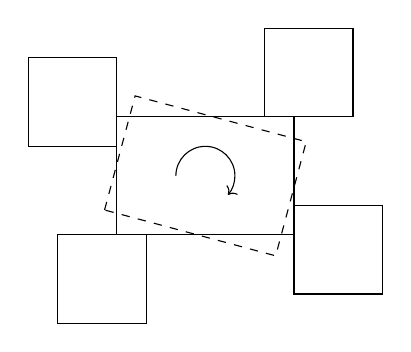
\begin{tikzpicture}[scale=0.75]
                \draw[] (0, 0) rectangle (3, 2);
                \draw[->] (1, 1) arc (180:-40:0.5);
                \draw[] (-1, -1.5) rectangle (0.5, 0);
                \draw[] (-1.5, 1.5) rectangle (0, 3);
                \draw[] (3, -1) rectangle (4.5, 0.5);
                \draw[] (2.5, 2) rectangle (4, 3.5);
                \draw[dashed, rotate around={-15:(1.5, 1)}] (0, 0) rectangle (3, 2);
            \end{tikzpicture}
        \caption{Rectangle which can not be translated, since it is wedged between two rectangles along each dimension. Observe however, that it \textit{can} be rotated.}
        \label{fig:wedged-and-loose}
    \end{subfigure}
    ~
    \begin{subfigure}[b]{0.45\textwidth}
        \centering
            \begin{tikzpicture}[scale=0.75]
                \draw[] (0, 0) rectangle (3, 2);
                \draw[] (0.5, -1.5) rectangle (2, 0);
                \draw[] (-1.5, 0.5) rectangle (0, 2);
                \draw[] (3, 0.25) rectangle (4.5, 1.75);
                \draw[] (1.5, 2) rectangle (3, 3.5);
                \draw[dashed] (-1.75, 0.75) -- (4.75, 0.75);
                \draw[dashed] (1.75, -1.75) -- (1.75, 3.75);

                \node at (0, 2) [anchor=north west] {$R_p$};
                \filldraw (1.75, 0.75) circle (2pt) node[anchor=north west] {$c$};
            \end{tikzpicture}
        \caption{Rectangle which can not be translated or rotated, since along each dimension there is a line passing through it and the adjacent rectangles.}
        \label{fig:wedged-with-line-fixed}
    \end{subfigure}
    \caption{Examples illustrating what is necessary to ensure that a hyperrectangle can not be moved.}
\end{figure}

\noindent Lastly, we consider the feasibility of moving multiple hyperrectangles simultaneously. Then in particular we move some specific hyperrectangle $R$. But moving $R$ forces us to also move some adjacent hyperrectangle to prevent overlap and this causes a chain reaction resulting in one of the hyperrectangles pricking a hole in the surrounding hypercube $C$ and thus no longer constituting a packing. Hence, without further ado we will state the following proposition.

\begin{proposition}\label[proposition]{prop:hoffman-packing-rigid}
Suppose $d$ is a dimension tuple satisfying Hoffman's inequality and suppose $(B, C)$ is a packing of $d$ consisting solely of hyperrectangles. Then $(B, C)$ is a rigid packing.
\end{proposition}

\noindent The following result limits the number of universal packings being equivalent.

\begin{lemma}\label[lemma]{lemma:finding-tuples}
There exists a strictly increasing sequence of $n$ positive real numbers $x_1 < x_2 < \dotsb < x_n$ such that $\paren{x_1, x_2, \dotsc, x_n}$ satisfies Hoffman's inequality and such that the only way to add an arbitrary number of these sequence elements up to $x_1 + x_2 + \dotsb + x_n$ is to add precisely one of each.
\end{lemma}
\begin{proof}
The case $n = 1$ is trivial, so suppose $n \geq 2$. Define a sequence of $n$ positive real numbers by $x_i = 1 + n^{-(n-i+1)}$ for $i = 1, 2, \dotsc, n$. Note that this sequence is strictly increasing since
\[
x_{i+1} - x_i
= n^{-(n-i)} - n^{-(n-i+1)}
= n^{-(n-i)}(1 - 1/n) > 0
\]
for all suitable $i$. We now represent each sequence element in base-$n$. Then the fractional part of $x_i$ consists of $n-i$ zeros followed by a one for all $i = 1, 2, \dotsc, n$, i.e.\ $x_n = 1.1_n$, $x_{n-1} = 1.01_n$ and so on. We denote the sum consisting of precisely one of each sequence element by $s$ and we see that
\[
s = x_1 + x_2 + \dotsb + x_n = 10.\overbrace{11 \dotso 1}^{\text{$n$ ones}}\!{}_n.
\]
Notice that any sum of sequence elements with more than $n$ terms will be strictly greater than $s$, since the integer part of the sum would be at least $11_n$. In particular, the sequence satisfies Hoffman's inequality.

Suppose there exists a sum of sequence elements with $n$ or fewer terms such that they add up to $s$. Consider the base-$n$ representation of this sum. Precisely one of the terms must be $x_1$, since this is the only way to obtain a one at the $n$'th position of the fractional part of the sum. Similarly, we can now conclude that precisely one term must be $x_2$ and using induction the sum must have $n$ terms with precisely one $x_i$ term for each $i = 1, 2, \dotsc, n$.
\end{proof}

\begin{lemma}\label[lemma]{lemma:distinct-hoffman-packings-different}
Suppose $d$ is a dimension tuple with distinct elements. If $P_1$ and $P_2$ are Hoffman packings of $d$ producing the same packing, then $P_1 = P_2$.
\end{lemma}
\begin{proof}
Let $(B, C)$ be the packing produced by $P_1$ and $P_2$. Suppose $p$ is a grid point coordinate in $G_n$. We would like to show that $P_1(p) = P_2(p)$. Consider the dimension tuple $r$ of the hyperrectangle $R_p$ in $B$ associated with $p$. Since the elements of $d$ are distinct there is only one permutation $\sigma$ in $S_n$ such that $(d_{\sigma(1)}, d_{\sigma(2)}, \dotsc, d_{\sigma(n)}) = r$, whereby $P_1(p) = \sigma = P_2(p)$.
\end{proof}

\begin{proposition}\label[proposition]{prop:universal-symmetries}
A unique universal packing contains at most $n! \cdot 2^n$ universal packings.
\end{proposition}
\begin{proof}
Suppose $\Omega$ is a unique universal packing. Let $d$ be the dimension tuple consisting of the sequence given by \cref{lemma:finding-tuples}. Then all of the Hoffman packings in $\Omega$ produce packings of $d$, which are equivalent. However, none of them are identical due to \cref{lemma:distinct-hoffman-packings-different}. By \cref{prop:hoffman-packing-rigid} these packings are rigid, so there are at most $n! \cdot 2^n$ of them, namely their symmetries. Thus, there are at most $n! \cdot 2^n$ Hoffman packings in $\Omega$.
\end{proof}

\subsection{Verifying a Hoffman packing}
When assessing whether a map $P \colon G_n \to S_n$ is in fact a universal packing we need to show that it is a Hoffman packing of any dimension tuple $d$ satisfying Hoffman's inequality. Therefore we seek a clever way of ensuring that the pseudo-packing $(B, C)$ produced by $P$ is in fact a packing of $d$. Hence, we need to make sure that all of the hyperrectangles in $B$ are contained in the surrounding hypercube $C$ and that the hyperrectangles in $B$ are pairwise non-overlapping. Let us begin with a criterion which ensures that the hyperrectangles are contained in the surrounding hypercube.

\begin{criterion}[Line criterion]\label[criterion]{criterion:line-criterion}\index{Criterion!line}
Suppose $P\colon G_n \to S_n$. Let $d = \paren{x_1, x_2, \dotsc, x_n}$ be a dimension tuple with distinct elements and consider the pseudo-packing $(B, C)$ of $d$ produced by $P$. A grid line along some dimension $k \in \curly{1, 2, \dotsc, n}$ is a \textit{unique line}\index{Grid line!unique} if for all $i = 1, 2, \dotsc, n$ there is precisely one grid point $p$ on the grid line where the associated hyperrectangle has an extent of $x_i$ along the $k$'th dimension, i.e.\ $P(p)(k) = i$. If all grid lines are unique lines, then $P$ satisfies the \textit{Line criterion}.
\end{criterion}

\begin{remark}
The Line criterion \labelcref{criterion:line-criterion} is inspired by Hoffman, who introduced it in the three-dimensional case \cite[p. 220]{Hoffman1981}. However, Hoffman's way of justifying it does not scale easily to higher dimensions. However, as we will see below, the notion of a universal packing does in fact allow us to require it in higher dimensions.
\end{remark}

\noindent It follows from the next result that the Line criterion \labelcref{criterion:line-criterion} will guarantee the hyperrectangles to be contained in the surrounding hypercube.

\begin{proposition}\label[proposition]{prop:under-stuffed-contains-rects}
Suppose $P \colon G_n \to S_n$. Let $d$ be a dimension tuple and let $s$ be its sum. Let $(B, C)$ be the pseudo-packing of $d$ produced by $P$. If the stuffing on each grid line is no bigger than $s$, then all of the hyperrectangles in $B$ are contained in the surrounding hypercube $C$.
\end{proposition}
\begin{proof}
Recall that $C = (0, s)^n$. Suppose $p$ is a grid point coordinate in $G_n$ and let $R_p$ denote the associated hyperrectangle in $B$. Using the notation from \cref{def:hoffman-packing}, we can write $R_p$ as the Cartesian product
\[
R_p = \prod_{i = 1}^n (a(p)_i, b(p)_i)
= (a(p)_1, b(p)_1) \times (a(p)_2, b(p)_2) \times \dotsb \times (a(p)_n, b(p)_n).
\]
Let $v$ be an element in $R_p$ and note that $a(p)_i < v_i < b(p)_i$ for all $i = 1, 2, \dotsc, n$. In order to show that $v$ lies in $C$, we need to show that $0 < v_i < s$ for all $i = 1, 2, \dotsc, n$.

Take some $i$ in $\curly{1, 2, \dotsc, n}$. By examining the definition of the $i$'th element of the anchor-point $a(p)$ in \cref{def:hoffman-packing}, we observe that $a(p)_i$ is a sum of non-negative real numbers. Hence, $a(p)_i$ is non-negative itself, whereby $0 \leq a(p)_i < v$. Next, consider $b(p)_i = a(p)_i + w(p)_i$, which can be recursively unwrapped into
\[
b(p)_i = \sum_{k = 1}^{p_i} w(L(p, i, k))_i \leq \sum_{k = 1}^{n} w(L(p, i, k))_i \leq s,
\]
since the stuffing on the grid line running through $p$ along dimension $i$ is no bigger than $s$. Then $v_i < b(p)_i \leq s$, so $v$ is in $C$. Thus, $R_p$ is contained in $C$ as desired.
\end{proof}

\noindent Next, we show that restricting the search for universal packings to maps $P\colon G_n \to S_n$ satisfying the Line criterion \labelcref{criterion:line-criterion} does not overlook any universal packings.

\begin{proposition}\label[proposition]{prop:universal-packing-has-unique-lines}
Suppose $P$ is a universal packing. Then $P$ satisfies the Line criterion \labelcref{criterion:line-criterion}.
\end{proposition}
\begin{proof}
Let $d = \paren{x_1, x_2, \dotsc, x_n}$ be the dimension tuple consisting of the sequence given by \cref{lemma:finding-tuples} and let $s$ denote its sum. Observe that the elements of $d$ are distinct, since it is strictly increasing. Let $(B, C)$ be the packing of $d$ produced by $P$. Take some grid line along some dimension $k \in \curly{1, 2, \dotsc, n}$. We would like to show that this is a unique line. Since $d$ satisfies Hoffman's inequality this grid line is completely stuffed by Hoffman's line theorem \labelcref{thm:line-theorem}. Recall that by \cref{lemma:finding-tuples} the only way to add the elements of $d$ up to $s$ is to use precisely one of each. There are $n$ grid points on the grid line, so for each $i = 1, 2, \dotsc, n$ there must be precisely one grid point $p_i$ on the grid line for which the associated hyperrectangle has an extent of $x_i$ along the $k$'th dimension, i.e.\ $P(p_i)(k) = i$. Hence, the grid line is a unique line, whereby $P$ satisfies the Line criterion \labelcref{criterion:line-criterion}.
\end{proof}

\noindent It remains to ensure that the hyperrectangles are pairwise non-overlapping. The naive approach would be to check every pair of hyperrectangles one by one. The next result indicates how such a check could be performed.

\begin{lemma}\label[lemma]{lemma:overlap}
Suppose $R_1 = I_1 \times I_2 \times \dotsb \times I_n$ and $R_2 = J_1 \times J_2 \times \dotsb \times J_n$ are two $n$-dimensional hyperrectangles. These two hyperrectangles are overlapping if and only if $I_k$ intersects $J_k$ for all $k = 1, 2, \dotsc, n$.
\end{lemma}
\begin{proof}
Suppose $R_1$ and $R_2$ are overlapping, i.e.\ they intersect one another. Then there exists a point $p$ in their intersection $R_1 \cap R_2$. Take any $k$ in $\curly{1, 2, \dotsc, n}$. Since $p$ is in $R_1$, then $p_k$ is in $I_k$. Similarly $p_k$ is in $J_k$. Hence, $I_k$ intersects $J_k$.

Suppose $I_k$ intersects $J_k$ for all $k = 1, 2, \dotsc, n$. Then there exists a real number $p_k$ in $I_k \cap J_k$ for all $k = 1, 2, \dotsc, n$. The point $p = \paren{p_1, p_2, \dotsc, p_n}$ is in both $R_1$ and $R_2$, so they intersect one another. Hence, $R_1$ and $R_2$ are overlapping.
\end{proof}
\noindent Thus, these two hyperrectangles are non-overlapping if and only if there is a $k$ in $\curly{1, 2, \dotsc, n}$ such that $I_k$ and $J_k$ are disjoint. It turns out that it is not necessary to check whether every pair of hyperrectangles are overlapping.

\begin{definition}[Neighbouring grid points]\index{Grid point!neighbouring}
Two grid points are \textit{neighbours} if their respective coordinates $p$ and $q$ satisfy
\[
\max_{i = 1}^n \, \abs{p_i - q_i} = 1.
\]
\end{definition}

\noindent It turns out that it is only necessary to ensure that hyperrectangles associated with neighbouring grid points are non-overlapping.

\begin{criterion}[No neighbour overlap criterion]\label[criterion]{criterion:no-neighbour-overlap-criterion}\index{Criterion!no neighbour overlap}
Suppose $P \colon G_n \to S_n$. Let $d$ be a dimension tuple and let $(B, C)$ be the pseudo-packing of $d$ produced by $P$. Then $P$ satisfies the \textit{No neighbour overlap criterion} for $d$ if for any pair of neighbouring grid point coordinates $p$ and $q$ in $G_n$ there exists a $k$ in $\curly{1, 2, \dotsc, n}$ with $p_k \neq q_k$ such that
\begin{align*}
b(p)_k \leq a(q)_k &\quad \text{if } p_k < q_k \\
b(q)_k \leq a(p)_k &\quad \text{if } p_k > q_k,
\end{align*}
where $a(p)$ and $a(q)$ are the anchor points, whereas $b(p)$ and $b(q)$ are the right interval endpoints (as defined in \cref{def:hoffman-packing}) of the hyperrectangles $R_p$ and $R_q$ associated with $p$ and $q$, respectively.
\end{criterion}

\noindent The above criterion ensures that the $k$'th interval in the Cartesian product of $R_p$ does not intersect the corresponding interval of $R_q$, whereby the two hyperrectangles are non-overlapping by \cref{lemma:overlap}.

\begin{remark}
The No neighbour overlap criterion \labelcref{criterion:no-neighbour-overlap-criterion} is inspired by Hoffman's observation that a ``sharp corner'' such as the one in \cref{fig:3d-sharp-corner-square} may not occur \cite[p. 221]{Hoffman1981}. However, we have found that this concept of a sharp corner extends to higher dimensions, such as the one in \cref{fig:3d-sharp-corner-cube}. The above criterion encodes the necessary information to detect any type of sharp corner as soon as it emerges.
\begin{figure}[ht]
    \centering
    \begin{subfigure}[b]{0.47\textwidth}
        \centering
            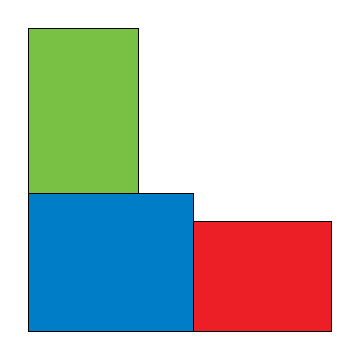
\begin{tikzpicture}[scale=0.35]
                \filldraw[fill=custom-blue, draw=black] (0,0) rectangle (6,5);
\filldraw[fill=custom-green, draw=black] (0,5) rectangle (4,11);
\filldraw[fill=custom-red, draw=black] (6,0) rectangle (11,4);
            \end{tikzpicture}
        \caption{Sharp corner in two dimensions.}
        \label{fig:3d-sharp-corner-square}
    \end{subfigure}
    ~
    \begin{subfigure}[b]{0.47\textwidth}
        \centering
            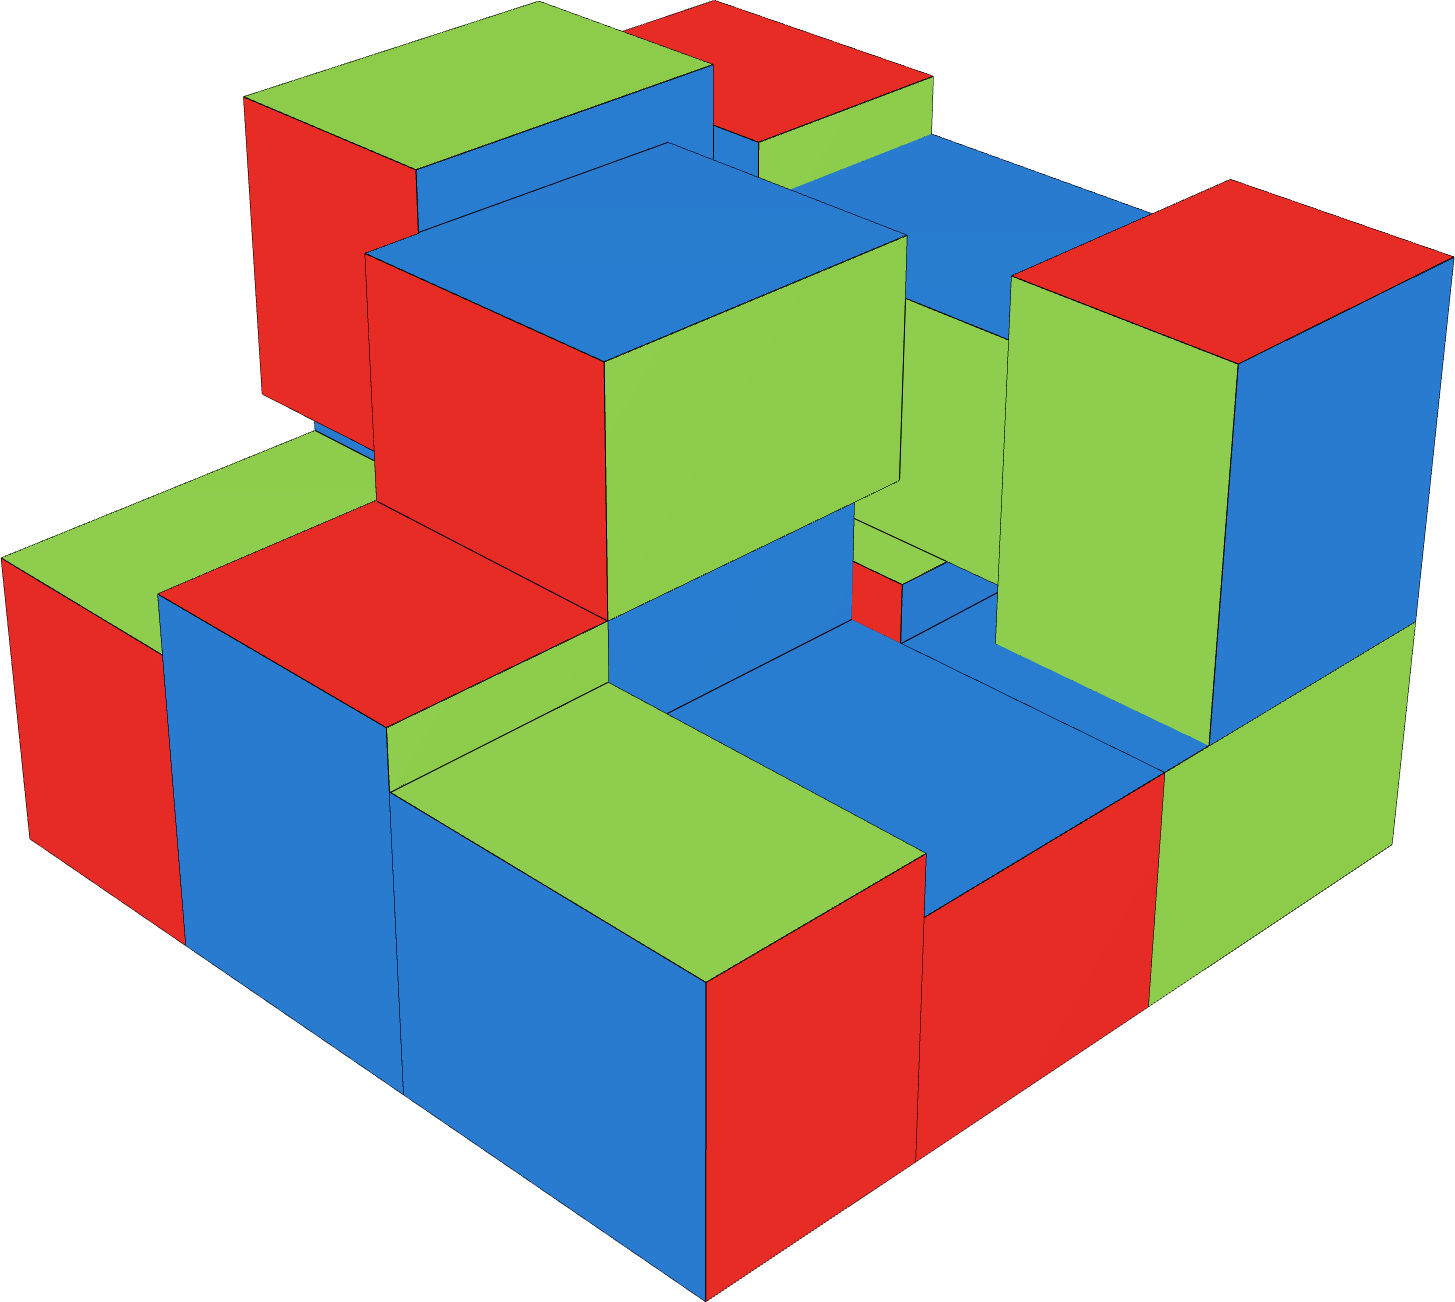
\includegraphics[scale=0.23]{graphics/3d-cube-sharp-corner.png}
        \caption{Sharp corner in three dimensions.}
        \label{fig:3d-sharp-corner-cube}
    \end{subfigure}
    \caption{Examples of sharp corners. Observe that the three-dimensional sharp corner can not be detected by looking at the squares. Thus, while sharp corners of higher dimensions are theoretically possible, they are not easily visualized.}
    \label{fig:3d-sharp-corners}
\end{figure}
\end{remark}

\noindent The next result shows that the No neighbour overlap criterion \labelcref{criterion:no-neighbour-overlap-criterion} is satisfied by any Hoffman packing of a dimension tuple satisfying Hoffman's inequality.

\begin{proposition}\label[proposition]{prop:hoffman-packing-satisfies-nnoc}
Suppose $P\colon G_n \to S_n$ is a Hoffman packing of a dimension tuple $d$ satisfying Hoffman's inequality. Then $P$ satisfies the No neighbour overlap criterion \labelcref{criterion:no-neighbour-overlap-criterion} for $d$.
\end{proposition}
\begin{proof}
Let $(B, C)$ be the packing of $d$ produced by $P$. Suppose $p$ and $q$ are two neighbouring grid point coordinates in $G_n$ and let
\[
R_p = I_1 \times I_2 \times \dotsb \times I_n \quad \text{and} \quad
R_q = J_1 \times J_2 \times \dotsb \times J_n
\]
be their associated hyperrectangles in $B$. Let $\alpha$ and $\beta$ be the actual grid points corresponding to the coordinates $p$ and $q$, respectively. By Hoffman's grid theorem \labelcref{thm:grid-theorem} each grid point lies inside its respective hyperrectangle, i.e.\ $\alpha \in R_p$ and $\beta \in R_q$. Since $(B, C)$ is a packing $R_p$ and $R_q$ are non-overlapping, so by \cref{lemma:overlap} there exists some $k$ in $\curly{1, 2, \dotsc, n}$ such that $I_k$ does not intersect $J_k$. We must have that $\abs{p_k - q_k} = 1$, because otherwise $p_k = q_k$, whereby $\alpha_k = \beta_k$ and $I_k$ would intersect $J_k$. In the notation of the No neighbour overlap criterion \labelcref{criterion:no-neighbour-overlap-criterion} $I_k = (a(p)_k, b(p)_k)$ and $J_k = (a(q)_k, b(q)_k)$. If $p_k < q_k$, then $\alpha_k < \beta_k$. Then $b(p)_k \leq a(q)_k$ to avoid $I_k$ and $J_k$ intersecting one another. Similarly we conclude for $p_k > q_k$ that $b(q)_k \leq a(p)_k$. Hence, $P$ satisfies the No neighbour overlap criterion \labelcref{criterion:no-neighbour-overlap-criterion} for $d$.
\end{proof}

\noindent Next, we show that the No neighbour overlap criterion \labelcref{criterion:no-neighbour-overlap-criterion} and the Line criterion \labelcref{criterion:line-criterion} are enough to ensure that a pseudo-packing is in fact a packing. We will need the following result.

\begin{lemma}\label[lemma]{lemma:ordering-of-sum-by-terms}
Suppose $d = \paren{x_1, x_2, \dotsc, x_n}$ is a dimension tuple satisfying Hoffman's inequality and suppose $A$ and $B$ are two subsets of $D = \curly{1, 2, \dotsc, n}$. If $\abs{A} < \abs{B}$, then
\[
\sum_{i \in A} x_i < \sum_{i \in B} x_i.
\]
\end{lemma}
\begin{proof}
Suppose not.
Let $C = D \setminus A$. Recall that $d$ is increasing by Hoffman's inequality and note that $\abs{C} = n - \abs{A}$, so $\abs{B} + \abs{C} = \abs{B} + n - \abs{A} \geq n + 1$. Then
\begin{align*}
 x_1 + x_2 + \dotsb + x_n
= \sum_{i \in D} x_i
&= \sum_{i \in A} x_i + \sum_{i \in C} x_i \\
&\geq \sum_{i \in B} x_i + \sum_{i \in C} x_i
\geq (\abs{B} + \abs{C}) x_1
\geq (n + 1) x_1,
\end{align*}
which contradicts $d$ satisfying Hoffman's inequality.
\end{proof}

\noindent Intuitively, the sums consisting of distinct terms from $d$ are ordered by the number of terms in each sum. The situation gets significantly more complicated when two sums consist of the same number of terms, and we will return to this scenario in a moment.

\begin{theorem}\label[theorem]{thm:line-and-neighbour-gives-hoffman-packing}
Suppose $P \colon G_n \to S_n$ and suppose $d$ is a dimension tuple satisfying Hoffman's inequality. If $P$ satisfies the Line criterion \labelcref{criterion:line-criterion} and if $P$ satisfies the No neighbour overlap criterion \labelcref{criterion:no-neighbour-overlap-criterion} for $d$, then $P$ is a Hoffman packing of $d$.
\end{theorem}
\begin{proof}
Let $(B, C)$ be the pseudo-packing of $d$ produced by $P$. We need to show that $(B, C)$ is a packing of $d$. Let $s$ be the sum of $d$. Since $P$ satisfies the Line criterion \labelcref{criterion:line-criterion} the stuffing on each grid line is equal to $s$, i.e.\ all grid lines are completely stuffed. By \cref{prop:under-stuffed-contains-rects}, all hyperrectangles in $B$ are contained in the surrounding hypercube $C$. It only remains to show that the hyperrectangles in $B$ are pairwise non-overlapping.

Let $p$ and $q$ be two grid point coordinates in $G_n$ and let $R_p$ and $R_q$ denote their associated hyperrectangles. Next, consider the value of
\[
\delta = \max_{i = 1}^n \, \abs{p_i - q_i}.
\]
If $\delta = 0$, then $p = q$ and there is nothing to check. If $\delta = 1$, then $p$ and $q$ are neighbours and it follows by the No neighbour overlap criterion \labelcref{criterion:no-neighbour-overlap-criterion} that $R_p$ and $R_q$ are non-overlapping. Lastly, suppose $\delta > 1$. Then there exists some $k$ in $\curly{1, 2, \dotsc, n}$ such that $\abs{p_k - q_k} > 1$. Assume without loss of generality that $p_k < q_k$. Consider the $k$'th intervals $(a(p)_k, b(p)_k)$ and $(a(q)_k, b(q)_k)$ in the Cartesian products of $R_p$ and $R_q$, respectively. We would like to show that these do not intersect one another, which can be done by showing that $b(p)_k \leq a(q)_k$. By the construction of $(B, C)$ as described in \cref{def:hoffman-packing} the right endpoint $b(p)_k$ is a sum of $p_k$ terms from $d$, while the left endpoint $a(q)_k$ is a sum of $q_k - 1$ terms, namely
\[
b(p)_k = \sum_{i = 1}^{p_k} w(L(p, k, i))_k
\quad \text{and} \quad
a(q)_k = \sum_{i = 1}^{q_k - 1} w(L(q, k, i))_k.
\]
Since $P$ satisfies the Line criterion \labelcref{criterion:line-criterion}, each term in the sum for $b(p)_k$ can be identified by a distinct index in $\curly{1, 2, \dotsc, n}$. Denote this index set by $A$ and notice that $\abs{A} = p_k$. Similarly we get an index set for $B$ from the sum for $a(q)_k$ and $\abs{B} = q_k - 1$. Note that $\abs{A} = p_k < q_k - 1 = \abs{B}$, so by \cref{lemma:ordering-of-sum-by-terms} $b(p)_k < a(q)_k$. Then $R_p$ and $R_q$ are non-overlapping by \cref{lemma:overlap}. Thus, every pair of hyperrectangles are non-overlapping, so $(B, C)$ is a packing of $d$ and $P$ is a Hoffman packing of $d$.
\end{proof}

\noindent The above proof relies heavily on the dimension tuple $d$ satisfying Hoffman's inequality, where the technicalities have been buried in \cref{lemma:ordering-of-sum-by-terms}. However, experimental results suggest that we do not need to restrict ourselves to dimension tuples satisfying Hoffman's inequality and we will propose a conjecture in relation to this in \cref{sec:truely-universal-packing}.

\begin{remark}
Loosely speaking, Hoffman's inequality forces sums consisting of distinct terms from the increasing dimension tuple $\paren{x_1, x_2, \dotsc, x_n}$ to be ordered by the number of terms in each sum (\cref{lemma:ordering-of-sum-by-terms}). For $n = 3$ this property is actually guarded by the inequality
\begin{equation}\label{eq:3d-no-float-ineq}
    x_3 < x_1 + x_2,
\end{equation}
which Dean G. Hoffman drew our attention to in recent correspondences \cite{hoffman_private}. Observe that any dimension tuple $\paren{x_1, x_2, x_3}$ satisfying Hoffman's inequality will also satisfy \eqref{eq:3d-no-float-ineq}. However, $d' = \paren{2, 3, 4}$ satisfies \eqref{eq:3d-no-float-ineq}, but not Hoffman's inequality. Hence, the conclusion of \cref{lemma:ordering-of-sum-by-terms} and \cref{thm:line-and-neighbour-gives-hoffman-packing} should also hold for $d'$. We suspect the generalization of \eqref{eq:3d-no-float-ineq} to higher dimensions to be
\[
\sum_{i = \ceil*{n/2}+1}^{n} x_i < \sum_{i = 1}^{\ceil*{n/2}} x_i,
\]
and we mention this generalized inequality for future studies, because we suspect it to be a more precise requirement for a packing produced by a Hoffman packing to be rigid, i.e.\ without any ``loose bricks''.
\end{remark}

\subsection{Promoting a Hoffman packing to a universal packing}
By \cref{thm:line-and-neighbour-gives-hoffman-packing} we can guarantee that a map $P\colon G_n \to S_n$ is a universal packing by making sure that it satisfies the Line criterion \labelcref{criterion:line-criterion} and that it satisfies the No neighbour overlap criterion \labelcref{criterion:no-neighbour-overlap-criterion} for any choice of dimension tuple satisfying Hoffman's inequality. This is a lot of dimension tuples to examine and gives rise to the following definition.

\begin{definition}[Representative dimension tuple set]\label[definition]{def:representative-dimension-tuple-set}\index{Dimension tuple!representative set (RDTS)}
Suppose $T$ is a set of increasing dimension tuples. Then $T$ is a \textit{representative dimension tuple set} (RDTS)\index{RDTS|see{Dimension tuple}} if it has the following property: Suppose $P\colon G_n \to S_n$ satisfies the Line criterion \labelcref{criterion:line-criterion} and satisfies the No neighbour overlap criterion \labelcref{criterion:no-neighbour-overlap-criterion} for all dimension tuples in $T$, then $P$ satisfies the No neighbour overlap criterion \labelcref{criterion:no-neighbour-overlap-criterion} for \textit{any} increasing dimension tuple.
\end{definition}

\noindent We can restrict ourselves to maps satisfying the Line criterion \labelcref{criterion:line-criterion}, since it is a requirement for being a universal packing by \cref{prop:universal-packing-has-unique-lines}. Observe that the set of all increasing dimension tuples constitute a RDTS. However, it turns out that far fewer dimension tuples are required to constitute a RDTS. This greatly simplifies the practical search for universal packings, since it enables us to search for universal packings using just a few specific dimension tuples.

Suppose $P\colon G_n \to S_n$ is a map satisfying the Line criterion \labelcref{criterion:line-criterion}. If $P$ satisfies the No neighbour overlap criterion \labelcref{criterion:no-neighbour-overlap-criterion} for all dimension tuples in a RDTS, then it will in fact be a universal packing by \cref{thm:line-and-neighbour-gives-hoffman-packing}. When constructing a RDTS $T$ the strategy will be to include just enough dimension tuples to force $P$ to satisfy the No neighbour overlap criterion \labelcref{criterion:no-neighbour-overlap-criterion} for any choice of increasing dimension tuple as long as $P$ satisfies this criterion for the dimension tuples in $T$.

Suppose $d = \paren{x_1, x_2, \dotsc, x_n}$ is an increasing dimension tuple and let us examine the No neighbour overlap criterion \labelcref{criterion:no-neighbour-overlap-criterion} in more depth. For each pair of neighboring grid point coordinates $p$ and $q$ in $G_n$ the No neighbour overlap criterion \labelcref{criterion:no-neighbour-overlap-criterion} considers a number of inequalities, namely one for each entry where $p$ and $q$ differ. We will refer to such a composition of inequalities as an \textit{overlap comparison}\index{Overlap comparison} and to each of the inequalities as an \textit{overlap inequality}. Consider an overlap inequality from the overlap comparisons of $p$ and $q$. Notice that it has the same number of terms $t$ from $d$ on each side of the inequality sign and that $0 < t < n$. We will refer to the positive integer $t$ as the \textit{arity} of the overlap inequality. Consider the terms on one side. Since $P$ satisfies the Line criterion \labelcref{criterion:line-criterion}, then each term $x_i$ on this side is identified by a unique $i$ in $\curly{1, 2, \dotsc, n}$. Hence, we can identify an overlap inequality in the following way.

\begin{definition}[Overlap inequality]\label[definition]{def:overlap-inequality}\index{Overlap inequality}
Suppose $A$ and $B$ are two non-empty proper subsets of $\curly{1, 2, \dotsc, n}$ with the same cardinality $\abs{A} = \abs{B} = t$. Then $(A, B)$ is an $n$-dimensional \textit{overlap inequality} with \textit{arity}\index{Overlap inequality!arity of} $t$.
\end{definition}

\noindent We say that the dimension tuple $d$ \textit{satisfies}\index{Overlap inequality!satisfied by dimension tuple}\index{Dimension tuple!satisfying overlap inequality} the overlap inequality if
\[
\sum_{i \in A} x_i \leq \sum_{i \in B} x_i.
\]
Be aware that for the sake of readability, we might sometimes write an overlap inequality as above, even if each $x_i$ have not been defined.

Some overlap inequalities are satisfied for any choice of increasing dimension tuple. Suppose $(A, B)$ is an $n$-dimensional overlap inequality with arity $t$. Let $(\alpha_i)_{i=1}^t$ and $(\beta_i)_{i=1}^t$ be the strictly increasing sequences of element in $A$ and $B$, respectively. If $\alpha_i \leq \beta_i$ for all $i = 1, 2, \dotsc, t$, then the overlap inequality is satisfied by any increasing dimension tuple. We will refer to such an overlap inequality as \textit{trivial}\index{Overlap inequality!trivial}. It is convenient to introduce the following equivalence relation between $n$-dimensional increasing dimension tuples. Suppose $d_1 = \paren{x_1, x_2, \dotsc, x_n}$ and $d_2 = \paren{y_1, y_2, \dotsc, y_n}$ are two increasing dimension tuples. We define these dimension tuples to be equivalent if they satisfy the same overlap inequalities, that is for any non-empty proper subsets $A$ and $B$ of $\curly{1, 2, \dotsc, n}$ with $\abs{A} = \abs{B}$, then
\[
\sum_{i \in A} x_i \leq \sum_{i \in B} x_i
\iff
\sum_{i \in A} y_i \leq \sum_{i \in B} y_i.
\]
We denote the equivalence class of $d_1$ by $[d_1]$. Then we can establish a well-defined partial ordering on the equivalence classes, where $[d_1] \leq [d_2]$ if any overlap inequality satisfied by $d_1$ is also satisfied by $d_2$, that is
\[
\sum_{i \in A} x_i \leq \sum_{i \in B} x_i
\implies
\sum_{i \in A} y_i \leq \sum_{i \in B} y_i.
\]
Notice that the equivalence class $[\paren{x_1, x_2, \dotsc, x_n}]$ where $x_1 = x_2 = \dotsb = x_n$ containing the dimension tuple of any hypercube is the greatest element with respect to this ordering, since it satisfies all overlap inequalities. The next result shows how this partial ordering enables us to propagate information about the No neighbour overlap criterion \labelcref{criterion:no-neighbour-overlap-criterion}.

\begin{proposition}\label[proposition]{prop:propagate-nnoc}
Suppose $d_1$ and $d_2$ are two increasing dimension tuples with $[d_1] \leq [d_2]$. If $P\colon G_n \to S_n$ satisfies the Line criterion \labelcref{criterion:line-criterion} and satisfies the No neighbour overlap criterion \labelcref{criterion:no-neighbour-overlap-criterion} for $d_1$, then it does so for $d_2$ as well.
\end{proposition}
\begin{proof}
Since $P$ satisfies the Line criterion \labelcref{criterion:line-criterion} all overlap comparisons consist of inequalities which can be identified as in \cref{def:overlap-inequality}. Since $[d_1] \leq [d_2]$ the overlap inequalities satisfied by $d_1$ are satisfied by $d_2$ as well. Then $P$ satisfies the No neighbour overlap criterion \labelcref{criterion:no-neighbour-overlap-criterion} for $d_2$.
\end{proof}

\noindent The construction of these equivalence classes enables us to show the following result.

\begin{proposition}
The number of equivalence classes of increasing dimension tuples is finite.
\end{proposition}
\begin{proof}
Let us begin by establishing an upper bound on the number of different overlap inequalities. First, we count the number of overlap inequalities with a certain arity. Pick some arity $t$ and note that $0 < t < n$. The number of subsets of $\curly{1, 2, \dotsc, n}$ with $t$ elements is $\binom{n}{t}$, so the number of overlap inequalities with arity $t$ is $\binom{n}{t}^2$. Hence the total number of overlap inequalities is
\[
k = \sum_{i = 1}^{n - 1} \binom{n}{i}^n.
\]
When determining which equivalence class an increasing dimension tuple belongs to it depends on which overlap inequalities are satisfied and which are not. Hence, the number of equivalence classes is no greater than $2^k$.
\end{proof}

\noindent This information implies that there exists a finite RDTS in any dimension $n$, since we can construct such a set by picking a representative from each of the finitely many equivalence classes. We can actually show that any equivalence class has a representative satisfying Hoffman's inequality. Having a RDTS consisting of dimension tuples all satisfying Hoffman's inequality simplifies the search for a universal packing due to \cref{prop:hoffman-packing-satisfies-nnoc}.

\begin{proposition}\label[proposition]{prop:exists-representative-satisfying-hoffman-ineq}
Suppose $d$ is an increasing dimension tuple. Then there exists a dimension tuple $d'$ satisfying Hoffman's inequality and such that $[d] = [d']$.
\end{proposition}
\begin{proof}
Let $d = \paren{x_1, x_2, \dotsc, x_n}$ and let $c = \sum_{i = 1}^n \paren{x_i - x_1}$ and note that $c \geq 0$. Let $d' = \paren{y_1, y_2, \dotsc, y_n}$ where $y_i = x_i + c$ for all $i = 1, 2, \dotsc, n$. Note that for any overlap inequality $(A, B)$
\[
\sum_{i \in A} x_i \leq \sum_{i \in B} x_i \iff
\sum_{i \in A} \paren{x_i + c} \leq \sum_{i \in B} \paren{x_i + c} \iff
\sum_{i \in A} y_i \leq \sum_{i \in B} y_i,
\]
since $\abs{A} = \abs{B}$, whereby $[d] = [d']$. Next, we see that
\[
\sum_{i = 1}^n \paren{y_i - y_1} =
\sum_{i = 1}^n \paren{x_i - x_1} =
c < x_1 + c = y_1,
\]
and it follows that $d'$ satisfies Hoffman's inequality as desired.
\end{proof}

\noindent In addition, we can do better in order to reduce the number of dimension tuples necessary to constitute a RDTS.

\begin{proposition}\label[proposition]{prop:minimal-rdts}
Suppose $T$ is a set of increasing dimension tuples such that $T$ contains a representative from each minimal equivalence class. Then $T$ is a RDTS.
\end{proposition}
\begin{proof}
Suppose $P\colon G_n \to S_n$ satisfies the Line criterion \labelcref{criterion:line-criterion} and satisfies the No neighbour overlap criterion \labelcref{criterion:no-neighbour-overlap-criterion} for all dimension tuples in $T$. Suppose $d$ is an increasing dimension tuple. By the construction of $T$ there must be some dimension tuple $d'$ in $T$ such that $[d'] \leq [d]$. Since $P$ satisfies the No neighbour overlap criterion \labelcref{criterion:no-neighbour-overlap-criterion} for $d'$, then by \cref{prop:propagate-nnoc} it does so for $d$ as well. Hence, $T$ is a RDTS.
\end{proof}

\noindent Thus, if we can show that some equivalence class is in fact the least element, then the set consisting of just one of the dimension tuples from this equivalence class will constitute a RDTS. Next, we show a result which simplifies determining a small RDTS, and give an example of using it in the two-dimensional case.

\begin{proposition}\label[proposition]{prop:arity-1-trivial}
Suppose $d$ is an increasing dimension tuple with distinct elements. Then any overlap inequality with arity 1 satisfied by $d$ is trivial.
\end{proposition}
\begin{proof}
Let $d = \paren{x_1, x_2, \dotsc, x_n}$ and observe that it must be strictly increasing. Suppose $(A, B)$ is an overlap inequality with arity 1, i.e.\ $A$ and $B$ are non-empty proper subsets of $\curly{1, 2, \dotsc, n}$ with $\abs{A} = \abs{B} = 1$. Then we can write $A = \curly{i}$ and $B = \curly{j}$ for some $i$ and $j$ in $\curly{1, 2, \dotsc, n}$. If $i \leq j$, then the overlap inequality is trivial. Suppose not, i.e. $i > j$. Then $x_i \leq x_j$, which contradicts $d$ being strictly increasing.
\end{proof}

\begin{example}[RDTS for $n = 2$]
In this case all overlap inequalities have arity $1$. For an increasing dimension tuple $(x_1, x_2)$ there are four overlap inequalities,
\[
x_1 \leq x_1, \quad x_1 \leq x_2, \quad x_2 \leq x_1 \quad \text{and} \quad x_2 \leq x_2.
\]
Three of these are trivial, while $x_2 \leq x_1$---strictly speaking identified by the tuple $(\curly{2}, \curly{1})$---is the only non-trivial overlap inequality. Observe that $d = \paren{2, 3}$ satisfies Hoffman's inequality and contains distinct elements. Then $d$ satisfies only trivial overlap inequalities by \cref{prop:arity-1-trivial}. Hence $[d]$ is the least element, so by \cref{prop:minimal-rdts}
\[
T = \curly{\paren{2, 3}}
\]
is a RDTS for $n = 2$.
\end{example}

\noindent Before considering the three-dimensional case, we will show that an overlap inequality with sufficiently high arity is actually an overlap inequality with a lower arity in disguise. Intuitively, it has so many terms on each side of the inequality sign that some identical terms must occur on both sides. Subtracting these terms from both sides yields an overlap inequality with lower arity, which is satisfied precisely when the original overlap inequality is satisfied.

\begin{lemma}\label[lemma]{lemma:arity-minus-common-terms}
Suppose $(A, B)$ is a non-trivial $n$-dimensional overlap inequality with arity $s$. Then there exists an overlap inequality $(A', B')$ with arity $s - \abs{A \cap B}$ which is satisfied precisely when $(A, B)$ is satisfied.
\end{lemma}
\begin{proof}
Note that $A \neq B$, since the overlap inequality is non-trivial. Let $C = A \cap B$, $A' = A \setminus C$ and $B' = B \setminus C$. Then
\[
\sum_{i \in A} x_i \leq \sum_{i \in B} x_i
\iff
\sum_{i \in A'} x_i + \sum_{i \in C} x_i \leq \sum_{i \in B'} x_i + \sum_{i \in C} x_i
\iff
\sum_{i \in A'} x_i \leq \sum_{i \in B'} x_i
\]
for any increasing dimension tuple $d = \paren{x_1, x_2, \dotsc, x_n}$. Finally, note that $\paren{A', B'}$ has arity $t = s - \abs{A \cap B}$ and that $0 < t$, since $\abs{A \cap B} < s$.
\end{proof}

\begin{proposition}\label[proposition]{prop:arity-reduction}
Suppose $(A, B)$ is an $n$-dimensional overlap inequality. Then there exists an overlap inequality $(A', B')$ with arity $t$ such that $0 < t \leq n/2$ and which is satisfied precisely when $(A, B)$ is satisfied.
\end{proposition}
\begin{proof}
If $n = 1$ there are no overlap inequalities, so suppose $n \geq 2$. Let $s$ be the arity of $(A, B)$, that is $s = \abs{A} = \abs{B}$. If $s \leq n/2$ we are done by choosing $(A', B')$ to be $(A, B)$. Suppose $s > n/2$. If $A = B$, then the overlap inequality is trivial and we can simply choose $(A', B') = (\curly{1}, \curly{1})$. Otherwise by \cref{lemma:arity-minus-common-terms} there exists an overlap inequality $(A', B')$ with arity $t = s - \abs{A \cap B}$ which is satisfied precisely when $(A, B)$ is satisfied. We claim that $t \leq n/2$. Otherwise $n/2 < t$ and
\[
n < 2t = 2s - 2\abs{A \cap B}
= \abs{A} + \abs{B} - 2\abs{A \cap B}
= \abs{A \cup B} - \abs{A \cap B}
\leq \abs{A \cup B},
\]
which is impossible as $A$ and $B$ are subsets of $\curly{1, 2, \dotsc, n}$ with only $n$ elements.
\end{proof}

\begin{example}[RDTS for $n = 3$]\label[example]{ex:3d-rdts}
In this case all overlap inequalities have arity $1$ or $2$. Observe that $d = \paren{4, 5, 6}$ satisfies Hoffman's inequality and contains distinct elements. Of the overlap inequalities with arity $1$, then $d$ satisfies only the trivial ones by \cref{prop:arity-1-trivial}. We will show that the same is the case for overlap inequalities with arity $2$. Suppose $(A, B)$ is an overlap inequality with arity $2$ which is satisfied by $d$. Then by \cref{prop:arity-reduction} there exists an overlap inequality $(A', B')$ with arity $1$ which is also satisfied by $d$. But then $(A, B)$ is trivial itself. Hence $d$ satisfies only trivial overlap inequalities, so $[d]$ is the least element and by \cref{prop:minimal-rdts}
\[
T = \curly{\paren{4, 5, 6}}
\]
is a RDTS for $n = 3$. Hence, we can use this specific dimension tuple when searching for three-dimensional universal packings.
\end{example}

\section{Experiments in the three-dimensional case}
\noindent Let us attempt to find all of the three-dimensional universal packings using a computer program. We seek an algorithm which outputs the maps from $G_3$ to $S_3$ which are universal packings. We will refer to such a map as a solution. However, in order to count the number of unique universal packings we will not count a solution if we have already counted an equivalent solution. In the three-dimensional case we will refer to the hyperrectangles as bricks. We will approach this task using two different approaches, namely dynamic programming/memoization and backtracking.

\subsection{Dynamic programming}
The idea behind dynamic programming \cite[p. 359]{cormen_leiserson_rivest_stein_2009} is to solve a problem by combining the solutions of a number of simpler subproblems. We solve each of these subproblems once and store their solutions. Whenever one of these subproblems occurs again, then instead of recomputing its solution, we will simply look it up. Thus, dynamic programming uses additional memory to save computation time. The idea of storing solutions to the subproblems instead of recomputing them is called ``memoization'' \cite[p. 365]{cormen_leiserson_rivest_stein_2009}.

In order to apply this method to our problem, we need to specify what our subproblems are. This leads to the definition of a subgrid.

\begin{definition}[Subgrid]\index{Subgrid}
Suppose $U$ is a subset of $G_n = \curly{1, 2, \dotsc, n}^n$ obtained by fixing $k$ entries of the elements in $G_n$ and let $m = n - k$. We say that $U$ is an $m$-dimensional \textit{subgrid} of $G_n$.
\end{definition}

\noindent Observe that a one-dimensional subgrid corresponds to a grid line. Suppose $U$ is an $m$-dimensional subgrid of $G_n$ and suppose $P\colon U \to S_n$. Given some $n$-dimensional dimension tuple, we can---without going into details---extend the procedure from the definition of a Hoffman packing to produce what we will refer to as a \textit{subpacking}\index{Subpacking} consisting of $m$-dimensional hyperrectangles. It is also straight forward to extend the notion of equivalent subpackings. We will refer to a subpacking as a line, square and cube if $m = 1, 2$ and $3$, respectively.

The first idea that springs to mind for applying dynamic programming to this problem is to first figure out every possible line and store these. Then use these lines to construct every possible square and store them. Finally, we use these squares to construct all possible cubes, that is all solutions to our problem.

\begin{observation}
Using a computer program we have produced all lines, squares and cubes of the dimension tuple $(4, 5, 6)$. The results are presented in \cref{table:3d-dp-counts}. There is one subtlety in relation to combining solutions of the subproblems. When we have constructed a line there are two options left for the width of each line segment when combining lines to construct a square. We will refer to this as \textit{specialization}\index{Specialization}. There are three line segments on a line, and hence there are really $6 \cdot 2^3 = 48$ specialized lines. Given a square there is only one option left for which height to assign each rectangle. Thus, in the three-dimensional case we can think of a square as already specialized.

\begin{table}[ht]
\centering
\caption{Number of lines, squares (satisfying the Subgrid criterion \labelcref{criterion:subgrid-criterion}) and cubes of the dimension tuple $(4, 5, 6)$. Numbers in parentheses state the counts ignoring symmetries.}
\label{table:3d-dp-counts}
\bgroup
\def\arraystretch{1.1}
\begin{tabular}{|c|c|c|}
\hline
Lines   & Squares  & Cubes     \\ \hline
$6$ (3) & $624$ (78) & $1\,008$ (21) \\ \hline
\end{tabular}
\egroup
\end{table}
\end{observation}

\subsection{Backtracking}
Backtracking is a method for solving a problem by incrementally constructing a candidate solution, but ``backtracking'' when we can predict that this candidate can not possibly be completed to a solution. The usefulness of this technique relies on being able to predict failure early on and that such a test is relatively quick to perform. This enables us to efficiently traverse the search tree and prune the branches along the way.

The immediate way to apply backtracking to this problem is by placing one brick at a time and every time testing whether it might still be possible to complete the partial candidate to a solution. If there is still hope, we carry on and place another brick. If not, we remove the latest brick and register this rejection. If all orientations of a brick have been rejected, we backtrack, that is we remove the second latest brick and register this rejection. If all $3^3 = 27$ bricks have been successfully placed we save the solution. In order to continue searching for more solutions we can remove the last brick and artificially register this as a rejection.

In practise we represent a brick by its anchor point and dimension tuple. Placing a brick corresponds to inserting this information into a three-dimensional array structure where each array index represents a grid point coordinate. In order to determine and assign an anchor point to the brick, we need the bricks ``before'' it to be assigned beforehand. We can ensure this by considering the lexicographical ordering of the grid point coordinates and placing the bricks according to this ordering.
\begin{figure}[ht]
    \centering
    \begin{tikzpicture}
        \begin{axis}[
            height=0.7\textwidth,
            width=\textwidth,
            xmin=0, xmax=330,
            ymin=0, ymax=30,
            xlabel=Iteration,
            ylabel=Number of bricks placed,
            grid=both,
            legend style={at={(0.99,0.018)},
            anchor=south east}
        ]

            \addplot+[
                draw=custom-red,
                mark=none,
                mark last,
                mark options={
                    scale=1,
                    fill=custom-red
                }
            ]
            table{data/backtrack-3d-simple.dat};
            \addlegendentry{Procedure A}

            \addplot+[
                draw=custom-green,
                mark=none,
                mark last,
                mark options={
                    scale=1,
                    fill=custom-green
                }
            ]
            table{data/backtrack-3d-corners.dat};
            \addlegendentry{Procedure B}

            \addplot+[
                draw=custom-blue,
                mark=none,
                mark last,
                mark options={
                    scale=1,
                    fill=custom-blue
                }
            ]
            table{data/backtrack-3d-subspaces.dat};
            \addlegendentry{Procedure C}

            \addplot+[
                draw=custom-orange,
                mark=none,
                mark last,
                mark options={
                    scale=1,
                    fill=custom-orange
                }
            ]
            table{data/backtrack-3d-corners-subspaces.dat};
            \addlegendentry{Procedure D}
        \end{axis}
    \end{tikzpicture}
    \caption{Plot of the number of bricks placed after a certain number of iterations in the three-dimensional case depending on the different test procedures. Here, we terminate as soon as a solution is found, i.e.\ 27 bricks have been successfully placed.}
    \label{fig:backtracking-3d}
\end{figure}
During the course of this project, it has been possible to gradually improve the predictive power of the procedure which tests whether a partial candidate can not possibly be completed into a solution. The four procedures tried out are described in \cref{table:backtracking-procedures}.
\begin{table}[ht]
\centering
\caption{Description of the four procedures used to predict whether a partial candidate can not possibly be completed.}
\label{table:backtracking-procedures}
\bgroup
\def\arraystretch{1.1}
\begin{tabular}{|c|p{0.7\textwidth}|}
\hline
Procedure  & Description \\ \hline
A & Checks whether the Line criterion \labelcref{criterion:line-criterion} is violated or whether two neighbouring bricks are overlapping. \\ \hline
B & Checks all from procedure A and also whether there are sharp corners like in \cref{fig:3d-sharp-corners}. \\ \hline
C & Checks all from procedure A and also whether the Subgrid criterion \labelcref{criterion:subgrid-criterion} is violated. \\ \hline
D & Checks all of the above. \\ \hline
\end{tabular}
\egroup
\end{table}
Procedure D is a notable improvement over the naive procedure A requiring 53\% fewer iterations to find a single solution and 42\% fewer iterations to traverse the entire search tree and find all solutions. The details can be found in \cref{table:backtracking-3d}. This improvement and the significance of the different criteria is illustrated in \cref{fig:backtracking-3d}. While the running times of the procedures are different, we choose to compare number of iterations, since this gives a better indication of the branch pruning capabilities.

\begin{table}[ht]
\centering
\caption{Number of iterations needed to find a single solution and all solutions, respectively, in the three-dimensional case depending on the different test procedures.}
\label{table:backtracking-3d}
\bgroup
\def\arraystretch{1.1}
\begin{tabular}{|l|c|c|c|c|}
\hline
Procedure  & A  & B & C & D \\ \hline
One solution  & $327$     & $313$     & $166$       & $152$         \\ \hline
All solutions & $646\,009$ & $500\,185$ & $471\,569$   & $371\,560$ \\ \hline
\end{tabular}
\egroup
\end{table}

\subsection{Results and analysis of solutions}

By \cref{ex:3d-rdts} the set $\curly{\paren{4, 5, 6}}$ is a RDTS for $n = 3$, so it follows by \cref{thm:line-and-neighbour-gives-hoffman-packing} that any unique Hoffman packing of $\paren{4, 5, 6}$ satisfying the Line criterion \labelcref{criterion:line-criterion} is in fact a unique universal packing.

\begin{observation}\label[observation]{obs:3d-universal-packings}
Using the dynamic programming and backtracking approaches both yielded the same number of unique Hoffman packings of the dimension tuple $\paren{4, 5, 6}$, namely 21. These are presented in \cref{appendix-A}. Thus, the answer to \cref{q:count} is 21 for $n = 3$. In fact, this enables us to give the first proof that $3$ is a good dimension in \cref{thm:three-is-good}.
\end{observation}

\noindent We can define the \textit{distance}\index{Universal packing!distance between} between two universal packings $P_1$ and $P_2$ as the smallest number of function values of $P_1$ which we need to alter (intuitively, the smallest number of hyperrectangles we need to modify) such that the resulting map is equivalent to $P_2$ for any dimension tuple satisfying Hoffman's inequality. This defines a metric $l$ on the unique universal packings.

\begin{observation}\label[observation]{obs:3d-distances}
We have computed the distances between representatives from each of the 21 unique universal packings in the three-dimensional case. It turns out that the distance between any two non-equivalent universal packings $P_1$ and $P_2$ satisfies $6 \leq l(P_1, P_2) \leq 17$. In fact for any universal packing $P$, there exists a non-equivalent universal packing $P'$ such that $l(P, P') = 6$. Intuitively, we can always remove up to 5 arbitrary bricks from a universal packing and still have only one way to complete this partial solution.
\end{observation}

\noindent The importance of the above observation is unclear. However, we mention it as we speculate that a future and more thorough examination might reveal more knowledge of the problem. It might also be rewarding to compare it to the analysis of the 21 unique universal packings in \cite[p. 913--915]{berlekamp_conway_guy_2004}.

Suppose $\sigma$ is a permutation in $S_n$. We say that a universal packing $P$ is \textit{stable}\index{Universal packing!stable under permutation} under the permutation $\sigma$ if $P'\colon G_n \to S_n$ defined by
\[
P'(p) = P(p) \circ \sigma
\]
for all $p$ in $G_n$ is a universal packing. Note that we can determine whether a unique universal packing exhibits such a property by examining a representative.

\begin{observation}
We have examined whether the 21 unique universal packings in the three-dimensional case are stable under any permutation from $S_3$. Trivially, all 21 universal packings are stable under the identity permutation. In addition, 17 (numbered 1--17 in \cref{appendix-A}) of the unique universal packings are stable under the reversing permutation, i.e.
\[
\sigma =
\begin{pmatrix}
  1 & 2 & 3 \\
  3 & 2 & 1
\end{pmatrix}.
\]
Note that performing this operation twice, will undo it, since $\sigma^2$ is the identity. This operation associates 16 of the unique universal packings in pairs, while one of the unique universal packings exhibits the remarkable property that performing this operation on a representative yields a universal packing, which is equivalent to the representative. This particular packing can be seen in \cref{fig:universal-packing-3d}. These results are consistent with \cite[p. 5]{Spiridonov_2003} and \cite[p. 914]{berlekamp_conway_guy_2004} where the phenomenon is described as ``duality'' of packings. Interestingly, by looking at the packings in \cref{appendix-A} we have also noticed that all of these packings contain the square seen in \cref{fig:3d-special-square} and we have checked that the remaining packings 18--21 do not. Also, we found that no universal packing is stable under any other permutation from $S_3$.
\end{observation}

\noindent The above observation shows that ``duality'' is not a necessary condition for being a universal packing, but we speculate that it might be possible to exploit this phenomenon to improve the branch pruning when searching for a solution in higher dimensions. Requiring this property and using procedure D, we found the 17 unique universal packings in $349\,027$ iterations, which is a reduction by 6\%. However, it did not reduce the number of iterations needed to find the first solution.

\subsection{Comparison of the two approaches}
Both implementations take a split second to complete their search. Let us consider the advantages of the backtracking approach as opposed to dynamic programming. First of all, backtracking is well suited for showing the existence of a solution, since it performs only the work needed to obtain it. This is certainly not the case for the gradual solving in the bottom-up dynamic programming approach, where all lines are produced, then all squares and so on. Also, the backtracking approach has a tiny memory footprint, since it does not store solutions to subproblems. This will also let the implementation take better advantage of the caching capabilities in modern computer processors.

Secondly, with backtracking it is possible to discard symmetries, i.e.\ different equivalent packings, early on. If $n$ is odd then any universal packing will have a hyperrectangle in its ``middle'' and we can discard all rotations by fixing this hyperrectangle. If $n$ is even then we can still somewhat reduce the number of symmetries by fixing a group of hyperrectangles around the ``middle'', but---as we will see in the four-dimensional case---we need to be careful to get this right. It is not clear how one should go about doing something similar using dynamic programming, since we do not know which symmetries of a subproblem might be needed to solve the more complex problem beforehand. Hence, we can not discard these until the end.

However, the backtracking approach has one major drawback, namely that it is very difficult to say something meaningful about its progress. Using dynamic programming it is possible to provide a somewhat reasonable estimate on the amount of work left as we will provide in the four-dimensional case later.

Another advantage of the dynamic programming approach is that it is well suited for parallelization, since subproblems of the same size can be solved independently. For instance multiple threads can work together to construct all squares. However, as we will see shortly in the four-dimensional case, attempting to reduce the number of symmetries naturally divides the problems into independent problems, which the backtracking approach might be best suited for.

\subsection{Producing a packing of any dimension tuple using universal packing}\label{sec:truely-universal-packing}
The motive behind introducing the notion of a universal packing was twofold. First, we wanted the number of packings to be independent of the choice of dimension tuple; and secondly, because for $n \leq 3$ such a packing actually provides a ``recipe'' for constructing a packing of \textit{any} increasing dimension tuple, thereby proving these dimensions to be good. We put forward the following conjecture.

\begin{conjecture}\label[conjecture]{conjecture:universal}
Suppose $P \colon G_n \to S_n$ is a universal packing. Then $P$ produces a packing of any increasing dimension tuple. In particular $n$ is a good dimension.
\end{conjecture}

\noindent The truth of this conjecture is not too important for $n = 4$, since we know $4$ to be a good dimension by \cref{thm:multiplication-of-packings}. However, it would enable us to relax the definition of a universal packing to better suit its name and also further justify our formulation of \cref{q:count}. But most importantly, for $n = 5$ and larger primes, this would help pave the way of showing such a dimension to be good. First, one would determine a RDTS of dimension tuples satisfying Hoffman's inequality, then find a Hoffman packing of all these (and satisfying the Line criterion \labelcref{criterion:line-criterion}). Finally, one would promote it to be a universal packing by \cref{thm:line-and-neighbour-gives-hoffman-packing} and the dimension of interest would be good by the conjecture above.

Proving the above conjecture loosely speaking comes down to showing that any pair of hyperrectangles in a pseudo-packing are non-overlapping under the assumption of the Line criterion \labelcref{criterion:line-criterion} and that any pair of hyperrectangles associated with neighbouring grid points are non-overlapping. Intuitively, this seems obvious. However, when producing a pseudo-packing of a dimension tuple not satisfying Hoffman's inequality, then the hyperrectangle associated with a grid point does not necessarily contain this grid point. Hence, the intuition of ``neighbouring hyperrectangles'' might be deceiving. Apart from this intuition, the basis for proposing this conjecture is that we prove it for $n \leq 3$ below and the failed attempt to disprove it in the four-dimensional case which is documented in \cref{obs:4d-universal-counterexamples}.

The following proof works for $n \leq 3$, but it does not seem very straightforward to generalize it to higher dimensions, since even the case $n = 3$ is quite tedious.

\begin{proof}[Proof of \cref{conjecture:universal} for $n \leq 3$]
The case $n = 1$ is trivial. If $n = 2$ the only universal packing (up to equivalence) is the one illustrated in \cref{fig:universal-packing-2d}, which clearly produces a packing of any increasing dimension tuple. Suppose $n = 3$ and suppose $d = \paren{x_1, x_2, x_3}$ is an increasing dimension tuple and let $(B, C)$ be the pseudo-packing of $d$ produced by $P$. Note that $P$ satisfies the Line criterion \labelcref{criterion:line-criterion} by \cref{prop:universal-packing-has-unique-lines}. Note that by \cref{prop:exists-representative-satisfying-hoffman-ineq} there exists a RDTS for consisting of dimension tuples satisfying Hoffman's inequality (for instance the one presented in \cref{ex:3d-rdts}). Hence, $P$ satisfies the No neighbour overlap criterion \labelcref{criterion:no-neighbour-overlap-criterion} for each of these dimension tuples by \cref{prop:hoffman-packing-satisfies-nnoc}. Since they constitute a RDTS, then $P$ must also satisfy this criterion for $d$.

Notice that the Line criterion \labelcref{criterion:line-criterion} guarantees that the hyperrectangles in $B$ will be contained in the surrounding hypercube $C$ by \cref{prop:under-stuffed-contains-rects}. Next, we show that the hyperrectangles are pairwise non-overlapping. Take two distinct grid point coordinates $p$ and $q$ in $G_3$ and let $R_p$ and $R_q$ denote their associated bricks in $B$. Let
\[
\delta = \max_{i = 1}^{n} \abs{p_i - q_i},
\]
and note that $\delta$ is either $1$ or $2$. If $\delta = 1$, then $p$ and $q$ are neighbours and we are done due to the No neighbour overlap criterion \labelcref{criterion:no-neighbour-overlap-criterion} being satisfied for $d$. Suppose $\delta = 2$. Now, we assume that $p_i < q_i$ for all suitable $i$ and consider only the following case of $\Delta = q - p$, namely
\[
\paren{2, 0, 0}, \quad \paren{2, 1, 0}, \quad \paren{2, 1, 1}, \quad
\paren{2, 2, 0}, \quad \paren{2, 2, 1} \quad \text{and} \quad \paren{2, 2, 2}.
\]
Observe that we can do so without loss of generality, since we can always reflect and/or rotate the packing such that we end up in one of the above cases.

In the following we use the same notation as in the construction of a Hoffman packing, i.e.\ for a grid point $g$ in $G_3$, then $a(g)$ and $b(g)$ are the left and right interval endpoints of the associated hyperrectangle $R_g$ and $w(g) = b(g) - a(g)$ is the dimension tuple of the hyperrectangle $R_g$.

First, observe that for $R_p$ and $R_q$ to be overlapping along a dimension $k \in \curly{1, 2, 3}$ where $\abs{p_k - q_k} = 2$, then $w(p)_k = x_3 = w(q)_k$. Otherwise if for instance $w(q)_k$ is either $x_1$ or $x_2$ then
\[
b(p)_k = w(p)_k \leq x_3 \leq x_1 + x_2 + x_3 - w(q)_k = a(q)_k.
\]
Hence, if we are in one of the three last case there can not be any overlap, since $p$ and $q$ differ by $2$ along two dimensions. Also, the first case $\Delta = \paren{2, 0, 0}$ is straightforward, since $b(p)_1 \leq a(q)_1$ by construction of the pseudo-packing.

Next consider $\Delta = \paren{2, 1, 0}$ and suppose for contradiction that $R_p$ and $R_q$ are overlapping. Then in particular
\[
a(q)_1 < b(p)_1 \quad \text{and} \quad a(q)_2 < b(p)_2.
\]
It is helpful to glance at \cref{fig:conj-n2} for this next bit. Consider the grid point coordinate $r = p + \paren{1, 1, 0} = q + \paren{-1, 0, 0}$. By the No neighbour overlap criterion \labelcref{criterion:no-neighbour-overlap-criterion}
\[
b(p)_1 \leq a(r)_1 \quad \text{or} \quad b(p)_2 \leq a(r)_2,
\]
but $b(p)_1 \leq a(r)_1$ can not be the case, since $a(r)_1 \leq b(r)_1 = a(q)_1 < b(p)_1$. Then $b(p)_2 \leq a(r)_2$ must be the case. Next, consider the grid point coordinate $s = p + \paren{1, 0, 0} = q + \paren{-1, -1, 0}$ and note that $b(s)_2 = a(r)_2$. Now, notice that
\[
a(q)_1 < b(p)_1 = a(s)_1 \leq b(s)_1
\quad \text{and} \quad
a(q)_2 < b(p)_2 \leq a(r)_2 = b(s)_2,
\]
which contradicts $P$ satisfying the No neighbour overlap criterion for $s$ and $q$.
\begin{figure}[ht]
    \centering
    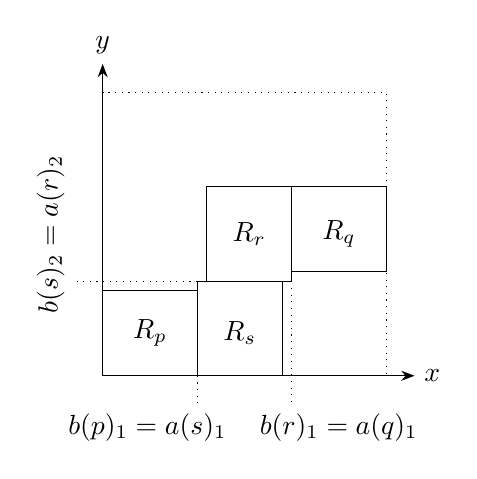
\begin{tikzpicture}[scale=1.2]
        \draw [-Stealth] (0, 0) -- ++(3.3, 0) node [right] {$x$};
        \draw [-Stealth] (0, 0) -- ++(0, 3.3) node [above] {$y$};

        \draw[dotted] (0, 0) -- ++(3, 0) -- ++(0, 3) -- ++(-3, 0) -- cycle;
        \draw (0, 0) -- ++(1, 0) -- ++(0, 0.9) -- ++(-1, 0) -- cycle;
        \draw (1, 0) -- ++(0.9, 0) -- ++(0, 1) -- ++(-0.9, 0) -- cycle;
        \draw (1.1, 1) -- ++(0.9, 0) -- ++(0, 1) -- ++(-0.9, 0) -- cycle;
        \draw (2, 1.1) -- ++(1, 0) -- ++(0, 0.9) -- ++(-1, 0) -- cycle;
        \node at (0.5, 0.45) {$R_p$};
        \node at (1.45, 0.45) {$R_s$};
        \node at (1.55, 1.5) {$R_r$};
        \node at (2.5, 1.5) {$R_q$};

        \draw[dotted] (1, 1) -- ++(-1.3, 0);
        \draw[dotted] (1, 0) -- ++(0, -0.3);
        \draw[dotted] (2, 1) -- ++(0, -1.3);

        \node [above, yshift=17pt, rotate=90] at (-0.3, 1) {$b(s)_2 = a(r)_2$};
        \node [below, xshift=-18pt] at (1, -0.3) {$b(p)_1 = a(s)_1$};
        \node [below, xshift=17pt] at (2, -0.3) {$b(r)_1 = a(q)_1$};
    \end{tikzpicture}
    \caption{Abstract relations between the interval endpoints of the bricks in the case $\Delta = \paren{2, 1, 0}$. This figure is highly distorted, since $R_p$ and $R_q$ are assumed to be overlapping in the proof.}
    \label{fig:conj-n2}
\end{figure}
Finally, consider the case $\Delta = \paren{2, 1, 1}$ and suppose for contradiction that $R_p$ and $R_q$ are overlapping. Note that $R_p$ and $R_q$ must be positioned in one of the two ways illustrated in \cref{fig:conj-n3}. First, consider the case illustrated in \cref{fig:conj-n3-corner} where $R_p$ is in a corner and $R_q$ is in the middle of the opposite side. Note that $w(p)_1 = w(q)_1 = x_3$ for these bricks to overlap along the $x$-axis. Then for the bricks to overlap along the $y$-axis $w(p)_2 = x_2$ and $a(q)_2 = x_1$. But then $w(p)_3 = x_1$ and $R_p$ can not be overlapping with $R_q$, since there is a brick below $R_q$ with a height of at least $x_1$.
\begin{figure}[ht]
    \centering
    \begin{subfigure}[b]{0.47\textwidth}
        \centering
            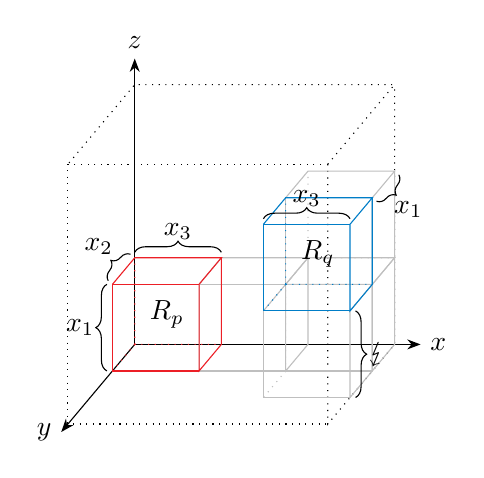
\begin{tikzpicture}[scale=1.1, z={(230:0.4cm)}]
                \boxfront{0}{0}{0}{3}{3}{3}{dotted}
                \draw [-Stealth] (0, 0, 0) -- ++(3.3, 0, 0) node [right] {$x$};
                \draw [-Stealth] (0, 0, 0) -- ++(0, 3.3, 0) node [above] {$z$};
                \draw [-Stealth] (0, 0, 0) -- ++(0, 0, 3.3) node [below, left] {$y$};

                \boxfront{2}{0}{1}{1}{1}{1}{lightgray}
                \boxback{2}{0}{1}{1}{1}{1}{lightgray, dotted}
                \boxfront{2}{0}{0}{1}{1}{1}{lightgray}
                \boxfront{1}{0}{0}{1}{1}{1}{lightgray}
                \boxfront{2}{1}{0}{1}{1}{1}{lightgray}
                \boxback{2}{1}{0}{1}{1}{1}{lightgray, dotted}

                \boxfront{0}{0}{0}{1}{1}{1}{custom-red}
                \boxback{0}{0}{0}{1}{1}{1}{custom-red, dotted}
                \node at (0.5, 0.5, 0.5) {$R_p$};

                \boxfront{2}{1}{1}{1}{1}{1}{custom-blue}
                \boxback{2}{1}{1}{1}{1}{1}{custom-blue, dotted}
                \node at (2.5, 1.5, 1.5) {$R_q$};

                \draw[decorate,decoration={brace, raise=2pt, amplitude=4pt}] (0, 1, 0) -- node[midway, above=3pt]{$x_3$} (1, 1, 0);
                \draw[decorate,decoration={brace, raise=2pt, amplitude=4pt, mirror}] (0, 1, 0) -- node[midway, xshift=-9pt, yshift=9pt]{$x_2$} (0, 1, 1);
                \draw[decorate,decoration={brace, raise=2pt, amplitude=4pt}] (0, 0, 1) -- node[midway, left=3pt]{$x_1$} (0, 1, 1);

                \draw[decorate,decoration={brace, raise=2pt, amplitude=4pt}] (2, 2, 2) -- node[midway, above=3pt]{$x_3$} (3, 2, 2);
                \draw[decorate,decoration={brace, raise=2pt, amplitude=4pt}] (3, 2, 0) -- node[midway, xshift=9pt, yshift=-9pt]{$x_1$} (3, 2, 1);
                \draw[decorate,decoration={brace, raise=2pt, amplitude=4pt, mirror}] (3, 0, 2) -- node[midway, right=3pt]{$\lightning$} (3, 1, 2);
            \end{tikzpicture}
        \caption{$R_p$ is in a corner and $R_q$ is in the middle of the opposite side.}
        \label{fig:conj-n3-corner}
    \end{subfigure}
    \hfill
    \begin{subfigure}[b]{0.47\textwidth}
        \centering
            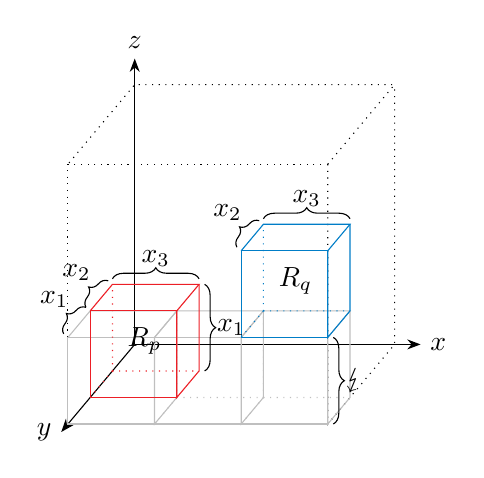
\begin{tikzpicture}[scale=1.1, z={(230:0.4cm)}]
                \boxfront{0}{0}{0}{3}{3}{3}{dotted}
                \draw [-Stealth] (0, 0, 0) -- ++(3.3, 0, 0) node [right] {$x$};
                \draw [-Stealth] (0, 0, 0) -- ++(0, 3.3, 0) node [above] {$z$};
                \draw [-Stealth] (0, 0, 0) -- ++(0, 0, 3.3) node [below, left] {$y$};

                \boxfront{0}{0}{2}{1}{1}{1}{lightgray}
                \boxfront{1}{0}{2}{1}{1}{1}{lightgray}
                \boxfront{2}{0}{2}{1}{1}{1}{lightgray}
                \boxback{1}{0}{2}{1}{1}{1}{lightgray, dotted}
                \boxback{2}{0}{2}{1}{1}{1}{lightgray, dotted}

                \boxfront{0}{0}{1}{1}{1}{1}{custom-red}
                \boxback{0}{0}{1}{1}{1}{1}{custom-red, dotted}
                \node at (0.5, 0.5, 1.5) {$R_p$};

                \boxfront{2}{1}{2}{1}{1}{1}{custom-blue}
                \boxback{2}{1}{2}{1}{1}{1}{custom-blue, dotted}
                \node at (2.5, 1.5, 2.5) {$R_q$};

                \draw[decorate,decoration={brace, raise=2pt, amplitude=4pt}] (0, 1, 1) -- node[midway, above=3pt]{$x_3$} (1, 1, 1);
                \draw[decorate,decoration={brace, raise=2pt, amplitude=4pt, mirror}] (1, 0, 1) -- node[midway, right=3pt]{$x_1$} (1, 1, 1);
                \draw[decorate,decoration={brace, raise=2pt, amplitude=4pt, mirror}] (0, 1, 1) -- node[midway, xshift=-9pt, yshift=9pt]{$x_2$} (0, 1, 2);
                \draw[decorate,decoration={brace, raise=2pt, amplitude=4pt, mirror}] (0, 1, 2) -- node[midway, xshift=-9pt, yshift=9pt]{$x_1$} (0, 1, 3);

                \draw[decorate,decoration={brace, raise=2pt, amplitude=4pt}] (2, 2, 2) -- node[midway, above=3pt]{$x_3$} (3, 2, 2);
                \draw[decorate,decoration={brace, raise=2pt, amplitude=4pt, mirror}] (2, 2, 2) -- node[midway, xshift=-9pt, yshift=9pt]{$x_2$} (2, 2, 3);
                \draw[decorate,decoration={brace, raise=2pt, amplitude=4pt, mirror}] (3, 0, 3) -- node[midway, right=3pt]{$\lightning$} (3, 1, 3);
            \end{tikzpicture}
        \caption{$R_p$ and $R_q$ are each in the middle of an edge.}
        \label{fig:conj-n3-edge}
    \end{subfigure}
    \caption{The two possible constellations of the bricks $R_p$ and $R_q$ in the case $\Delta = \paren{2, 1, 1}$. The figures are highly distorted, since $R_p$ and $R_q$ are assumed to be overlapping in the proof.}
    \label{fig:conj-n3}
\end{figure}

Next, consider the case illustrated in \cref{fig:conj-n3-edge} where $R_p$ and $R_q$ are each positioned in the middle of an edge. Again, along the $x$-axis $w(p)_1 = w(q)_1 = x_3$ for these bricks to overlap. Then for the bricks to overlap along the $y$-axis $w(q)_2 = x_2$ and the brick in front of $R_p$ must have an extent of $x_1$ along the $y$-axis. But then $w(p)_2 = x_2$, so $w(p)_3 = x_1$ and again $R_p$ can not be overlapping with $R_q$, since there is a brick below $R_q$ with a height of at least $x_1$. Hence, the bricks are pairwise non-overlapping, whereby $(B, C)$ is a packing of $d$ as desired.
\end{proof}

\begin{corollary}\label[corollary]{thm:three-is-good}
$3$ is a good dimension.
\end{corollary}

\begin{proof}
Take some representative $P$ of the 21 unique universal packings found in \cref{obs:3d-universal-packings}. Then by the proof above, $P$ produces a packing of any increasing dimension tuple. Hence, $P$ serves as a ``recipe'' for constructing a packing of \textit{any} dimension tuple, whereby $3$ is a good dimension.
\end{proof}

\section{Experiments in the four-dimensional case}
\noindent Let us examine the four-dimensional case. While the generalization of the problem to four dimensions is quite straightforward, the treatment of it is noticeably more difficult than that of lower dimensions. This is not only due to the greatly increased search space and subtle challenges in discarding symmetries. The real challenge arises from the fact that a RDTS must contain more than one dimension tuple. However, it took a long time to realize this and in order to get started, it was necessary to make a number of decisions, where the most appropriate choice was not obvious, simply because of the sparse knowledge of this problem.

Initially it seemed natural that examining any dimension tuple satisfying Hoffman's inequality and with distinct elements would represent the ``most difficult'' case. This is the line of thought presented by Spiridonov in \cite[p. 6]{Spiridonov_2003} and, after all, the immediate generalization of Hoffman's focus in \cite[p. 215]{Hoffman1981}. However, when attempting to count the number of four-dimensional squares it became clear that the number depended on the concrete choice of dimension tuple (satisfying Hoffman's inequality and with distinct elements). \cref{fig:4d-squares-good-bad} gives an example of a square without overlap for one of these dimension tuples, but with overlap for a different one.
\begin{figure}[ht]
    \centering
    \begin{subfigure}[b]{0.47\textwidth}
        \centering
            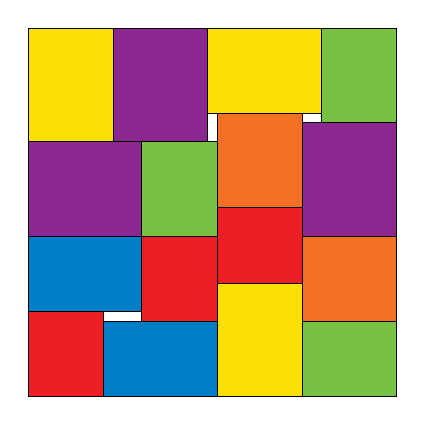
\begin{tikzpicture}[scale=0.12]
                \filldraw[fill=custom-red, draw=black] (0,0) rectangle (8,9);
\filldraw[fill=custom-blue, draw=black] (0,9) rectangle (12,17);
\filldraw[fill=custom-violet, draw=black] (0,17) rectangle (12,27);
\filldraw[fill=custom-yellow, draw=black] (0,27) rectangle (9,39);
\filldraw[fill=custom-blue, draw=black] (8,0) rectangle (20,8);
\filldraw[fill=custom-red, draw=black] (12,8) rectangle (20,17);
\filldraw[fill=custom-green, draw=black] (12,17) rectangle (20,27);
\filldraw[fill=custom-violet, draw=black] (9,27) rectangle (19,39);
\filldraw[fill=custom-yellow, draw=black] (20,0) rectangle (29,12);
\filldraw[fill=custom-red, draw=black] (20,12) rectangle (29,20);
\filldraw[fill=custom-orange, draw=black] (20,20) rectangle (29,30);
\filldraw[fill=custom-yellow, draw=black] (19,30) rectangle (31,39);
\filldraw[fill=custom-green, draw=black] (29,0) rectangle (39,8);
\filldraw[fill=custom-orange, draw=black] (29,8) rectangle (39,17);
\filldraw[fill=custom-violet, draw=black] (29,17) rectangle (39,29);
\filldraw[fill=custom-green, draw=black] (31,29) rectangle (39,39);
            \end{tikzpicture}
        \caption{Square of $\paren{8, 9, 10, 12}$ without overlap.}
    \end{subfigure}
    ~
    \begin{subfigure}[b]{0.47\textwidth}
        \centering
            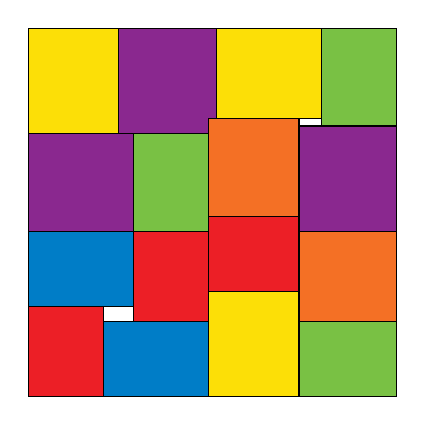
\begin{tikzpicture}[scale=0.12*39/49]
                \filldraw[fill=custom-red, draw=black] (0,0) rectangle (10,12);
\filldraw[fill=custom-blue, draw=black] (0,12) rectangle (14,22);
\filldraw[fill=custom-violet, draw=black] (0,22) rectangle (14,35);
\filldraw[fill=custom-yellow, draw=black] (0,35) rectangle (12,49);
\filldraw[fill=custom-blue, draw=black] (10,0) rectangle (24,10);
\filldraw[fill=custom-red, draw=black] (14,10) rectangle (24,22);
\filldraw[fill=custom-green, draw=black] (14,22) rectangle (24,35);
\filldraw[fill=custom-violet, draw=black] (12,35) rectangle (25,49);
\filldraw[fill=custom-yellow, draw=black] (24,0) rectangle (36,14);
\filldraw[fill=custom-red, draw=black] (24,14) rectangle (36,24);
\filldraw[fill=custom-orange, draw=black] (24,24) rectangle (36,37);
\filldraw[fill=custom-yellow, draw=black] (25,37) rectangle (39,49);
\filldraw[fill=custom-green, draw=black] (36,0) rectangle (49,10);
\filldraw[fill=custom-orange, draw=black] (36,10) rectangle (49,22);
\filldraw[fill=custom-violet, draw=black] (36,22) rectangle (49,36);
\filldraw[fill=custom-green, draw=black] (39,36) rectangle (49,49);
            \end{tikzpicture}
        \caption{Square of $\paren{10, 12, 13, 14}$ with overlap.}
    \end{subfigure}
    \caption{Example of the same square produced using two different dimension tuples. Using the second dimension tuple produces an overlap.}
    \label{fig:4d-squares-good-bad}
\end{figure}
This sudden overlap is due to a reliance on a non-trivial overlap inequality. Hence, it seemed appropriate to choose to completely exclude a partial solution if there is a pair of hyperrectangles where it relies solely on non-trivial overlap inequality to prevent overlap. This posed a problem, since---as we will see shortly---a four-dimensional dimension tuple will always satisfy at least one non-trivial overlap inequality. Hence, it was no longer possible to search for universal packings using a concrete dimension tuple, and this complicated the search considerably. However, this choice was later challenged by the discovery of a universal packing relying solely on non-trivial overlap inequalities for some of its overlap comparisons. It turns out that some non-trivial inequalities must be satisfied when others are not.
\begin{figure}[ht]
    \centering
    \begin{subfigure}[b]{0.47\textwidth}
        \centering
            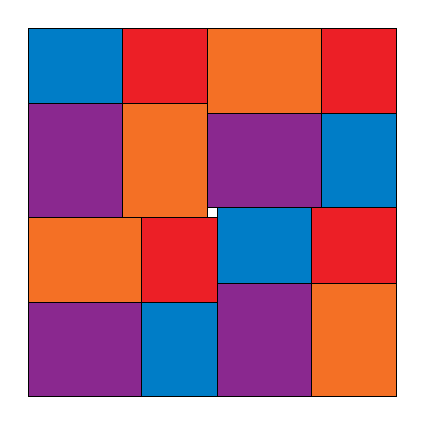
\begin{tikzpicture}[scale=0.12]
                \filldraw[fill=custom-violet, draw=black] (0,0) rectangle (12,10);
\filldraw[fill=custom-orange, draw=black] (0,10) rectangle (12,19);
\filldraw[fill=custom-violet, draw=black] (0,19) rectangle (10,31);
\filldraw[fill=custom-blue, draw=black] (0,31) rectangle (10,39);
\filldraw[fill=custom-blue, draw=black] (12,0) rectangle (20,10);
\filldraw[fill=custom-red, draw=black] (12,10) rectangle (20,19);
\filldraw[fill=custom-orange, draw=black] (10,19) rectangle (19,31);
\filldraw[fill=custom-red, draw=black] (10,31) rectangle (19,39);
\filldraw[fill=custom-violet, draw=black] (20,0) rectangle (30,12);
\filldraw[fill=custom-blue, draw=black] (20,12) rectangle (30,20);
\filldraw[fill=custom-violet, draw=black] (19,20) rectangle (31,30);
\filldraw[fill=custom-orange, draw=black] (19,30) rectangle (31,39);
\filldraw[fill=custom-orange, draw=black] (30,0) rectangle (39,12);
\filldraw[fill=custom-red, draw=black] (30,12) rectangle (39,20);
\filldraw[fill=custom-blue, draw=black] (31,20) rectangle (39,30);
\filldraw[fill=custom-red, draw=black] (31,30) rectangle (39,39);
            \end{tikzpicture}
        \caption{Square of $\paren{8, 9, 10, 12}$.}
    \end{subfigure}
    ~
    \begin{subfigure}[b]{0.47\textwidth}
        \centering
            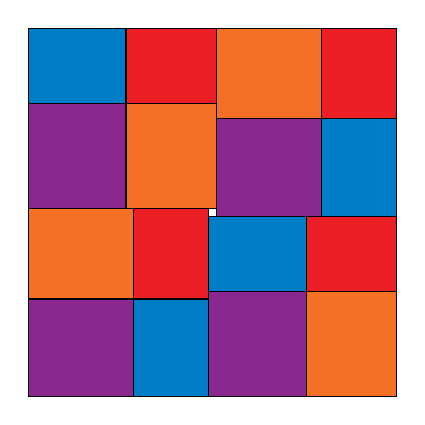
\begin{tikzpicture}[scale=0.12*39/49]
                \filldraw[fill=custom-violet, draw=black] (0,0) rectangle (14,13);
\filldraw[fill=custom-orange, draw=black] (0,13) rectangle (14,25);
\filldraw[fill=custom-violet, draw=black] (0,25) rectangle (13,39);
\filldraw[fill=custom-blue, draw=black] (0,39) rectangle (13,49);
\filldraw[fill=custom-blue, draw=black] (14,0) rectangle (24,13);
\filldraw[fill=custom-red, draw=black] (14,13) rectangle (24,25);
\filldraw[fill=custom-orange, draw=black] (13,25) rectangle (25,39);
\filldraw[fill=custom-red, draw=black] (13,39) rectangle (25,49);
\filldraw[fill=custom-violet, draw=black] (24,0) rectangle (37,14);
\filldraw[fill=custom-blue, draw=black] (24,14) rectangle (37,24);
\filldraw[fill=custom-violet, draw=black] (25,24) rectangle (39,37);
\filldraw[fill=custom-orange, draw=black] (25,37) rectangle (39,49);
\filldraw[fill=custom-orange, draw=black] (37,0) rectangle (49,14);
\filldraw[fill=custom-red, draw=black] (37,14) rectangle (49,24);
\filldraw[fill=custom-blue, draw=black] (39,24) rectangle (49,37);
\filldraw[fill=custom-red, draw=black] (39,37) rectangle (49,49);
            \end{tikzpicture}
        \caption{Square of $\paren{10, 12, 13, 14}$.}
    \end{subfigure}
    \caption{Example of square without overlap produced using two dimension tuples which satisfy different non-trivial overlap inequalities. This is surprising since the square relies on non-trivial overlap inequalities to prevent overlap.}
    \label{fig:4d-square-universal}
\end{figure}
\cref{fig:4d-square-universal} illustrates an effect of this phenomenon. Here there are no overlaps in either of the two squares, but for some pairs of hyperrectangle this is due to a gap along one dimension in the first square and a different dimension in the second square. This discovery is the true motivation behind introducing the notion of a RDTS and the elaborate machinery surrounding it.

\begin{example}[RDTS for $n = 4$]\label[example]{ex:4d-rdts}
In this case all overlap inequalities have arity $1$, $2$ or $3$. By \cref{prop:arity-reduction} we only have to consider the overlap inequalities with arity $1$ or $2$. We would like to choose a dimension tuple $\paren{x_1, x_2, x_3, x_4}$ satisfying Hoffman's inequality and containing distinct elements. Of the overlap inequalities with arity $1$, such a dimension tuple will only satisfy the trivial ones. If this is possible, then we only need to consider the overlap inequalities with arity $2$. Suppose $\paren{A, B}$ is a non-trivial overlap inequality with arity $2$. If $A \cap B \neq \emptyset$, then the inequality is really a non-trivial overlap inequality of arity $1$ in disguise by \cref{lemma:arity-minus-common-terms}. If $A \cap B = \emptyset$, then the only possibilities are
\[
x_1 + x_4 \leq x_2 + x_3 \quad
x_2 + x_3 \leq x_1 + x_4 \quad
x_2 + x_4 \leq x_1 + x_3
\quad \text{and} \quad
x_3 + x_4 \leq x_1 + x_2.
\]
However, if we choose dimension tuples with distinct elements, then the last two will not be satisfied. Thus, we are left with
\[
x_1 + x_4 \leq x_2 + x_3
\quad \text{and} \quad
x_2 + x_3 \leq x_1 + x_4.
\]
Observe that if one is not satisfied, then the other must be satisfied. However, it depends on the concrete choice of dimension tuple, whether only the first, only the second or both of them are satisfied. Observe that $d_1 = \paren{8, 9, 10, 12}$ and $d_2 = \paren{10, 12, 13, 14}$ both satisfy Hoffman's inequality and both contain distinct elements. Notice that $d_1$ does not satisfy the first overlap inequality, since $8 + 12 > 9 + 10$, while $d_2$ does not satisfy the second, since $12 + 13 > 10 + 14$. Hence $[d_1]$ and $[d_2]$ are the minimal elements and by \cref{prop:minimal-rdts}
\[
T = \curly{\paren{8, 9, 10, 12}, \paren{10, 12, 13, 14}}
\]
is a RDTS for $n = 4$. Intuitively, we have covered every possible way that we can linearly order the sums of two distinct terms (without any two sums with different terms being equal). This is illustrated in \cref{fig:hasse-4d-arity-2}.
\end{example}

\begin{figure}[ht]
    \centering
    \begin{subfigure}[b]{0.4\textwidth}
        \centering
            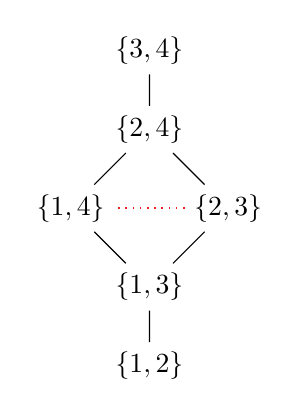
\begin{tikzpicture}[scale=1]
                \node (12) at (0,0) {$\curly{1, 2}$};
                \node (13) at (0,1) {$\curly{1, 3}$};
                \node (23) at (1,2) {$\curly{2, 3}$};
                \node (14) at (-1,2) {$\curly{1, 4}$};
                \node (24) at (0,3) {$\curly{2, 4}$};
                \node (34) at (0,4) {$\curly{3, 4}$};
                \draw (12) -- (13) -- (23) -- (24)
                      (13) -- (14) -- (24) -- (34);
                \draw [semithick, custom-red, dotted] (23) -- (14);
            \end{tikzpicture}
        \caption{The four-dimensional case.}
        \label{fig:hasse-4d-arity-2}
    \end{subfigure}
    ~
    \begin{subfigure}[b]{0.4\textwidth}
        \centering
            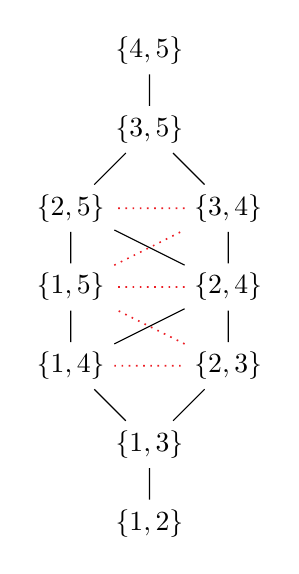
\begin{tikzpicture}[scale=1]
                \node (12) at (0,0) {$\curly{1, 2}$};
                \node (13) at (0,1) {$\curly{1, 3}$};
                \node (23) at (1,2) {$\curly{2, 3}$};
                \node (14) at (-1,2) {$\curly{1, 4}$};
                \node (24) at (1,3) {$\curly{2, 4}$};
                \node (15) at (-1,3) {$\curly{1, 5}$};
                \node (34) at (1,4) {$\curly{3, 4}$};
                \node (25) at (-1,4) {$\curly{2, 5}$};
                \node (35) at (0,5) {$\curly{3, 5}$};
                \node (45) at (0,6) {$\curly{4, 5}$};
                \draw (12) -- (13) -- (23) -- (24) -- (34) -- (35) -- (45)
                      (13) -- (14) -- (15) -- (25) -- (35)
                      (14) -- (24) -- (25);
                \draw [semithick, custom-red, dotted] (14) -- (23) -- (15) -- (34) -- (25)
                               (24) -- (15);
            \end{tikzpicture}
        \caption{The five-dimensional case.}
        \label{fig:hasse-5d-arity-2}
    \end{subfigure}
    \caption{Hasse diagrams of the partial ordering of sums with two distinct terms. Dotted lines represent relations which can not be determined in general. Each set $\curly{i, j}$ can by thought of as the sum $x_i + x_j$.}
\end{figure}

\begin{remark}\label[remark]{remark:bad-4d-tuple}
Spiridonov considers the dimension tuple $d = \paren{99, 100, 101, 102}$, because ``the sizes differ by a very small amount'' \cite[p. 6]{Spiridonov_2003}. Notice that $d$ satisfies both of the non-trivial overlap inequalities above as
$99 + 102 = 100 + 101$. Hence, if Spiridonov were to find a Hoffman packing of $d$, it might not produce a packing of neither $d_1$ nor $d_2$ in the example above. In particular, it might not be a universal packing.
\end{remark}

\subsection{Utilizing approaches from the three-dimensional case}
\noindent Let us begin by considering the dynamic programming approach.

\subsubsection{Dynamic programming}
We have used the dynamic programming approach to construct all squares in the four-dimensional case using the same strategy as in the three-dimensional case, that is by first constructing all lines and then combining them into squares. Note that this time a square is not automatically specialized as it was in the three-dimensional case.

\begin{observation}\label[observation]{obs:4d-dynamic-programming}
There are $4! = 24$ possible lines and if we specify one more dimension there are $24 \cdot 3^4 = 1\,944$. Using dynamic programming we have determined that there are $S = 51\,247\,458$ squares of the RDTS from \cref{ex:4d-rdts} without overlaps and satisfying the Line criterion \labelcref{criterion:line-criterion}. Observe that our count is different from---and quite a bit lower---than the $77\,436\,138$ squares counted by Spiridonov \cite[p. 6]{Spiridonov_2003} using the dimension tuple, which we questioned the choice of in \cref{remark:bad-4d-tuple}. We have reproduced his results for that choice of dimension tuple, but we still maintain that $S$ is the appropriate number due to its independence of the choice of dimension tuple.
\end{observation}

\noindent It takes a few minutes to generate all of the squares in the four-dimensional case and as we will see below, constructing all cubes does not seem to be practically possible for now. Let us attempt to estimate the number of cubes in the four-dimensional case and the computations needed to determine the exact number, if we construct them by stacking four squares. We only consider the consequences of the Line criterion \labelcref{criterion:line-criterion}, since it is difficult to predict overlap.

First, let us consider how many ways we can specialize the $4^2 = 16$ rectangles in a single square. There are two choices for each one, giving $2^{16}$ possible specializations. Hence, letting $S$ be defined as in \cref{obs:4d-dynamic-programming} there are $2^{16} S$ ways to choose the first square. Next, we would like to stack a second specialized square on top of it. For simplicity and due to the inclusion of symmetries we suppose that there is a $3/4$ probability that the heights of two bricks on top of each other will be different, so we estimate around $(3/4)^{16} 2^{16} S$ specialized squares to be compatible with the first choice. Hence, we estimate there to be around $(3/4)^{16} 2^{32} S^2 = 3^{16} S^2$ half-cubes. At his point, the half-cubes are presumably so constrained by the Line criterion \labelcref{criterion:line-criterion} that we consider an estimate of the number of compatible squares for the third square as too much guesswork. However, we can classify the half-cubes into $6^{16}$ groups depending on the $\binom{4}{2} = 6$ different ways to choose the brick heights in each of the $16$ stacks of two bricks. Under the assumption that the half-cubes distribute evenly into these groups, we estimate that one can exhaust the search space by checking
\[
\paren{3^{16} S^2}^2 6^{-16} \approx 4.5 \cdot 10^{33}
\]
different combinations of four squares. It is difficult to predict how many of these will have overlapping bricks. We have found $U = 1\,119\,514\,176$ different squares satisfying the Line criterion \labelcref{criterion:line-criterion}, if we do not check for overlaps while only $S/U \approx 4.58\%$ are in fact without overlapping bricks. Since there are more possibilities for overlaps in a cube, we suspect the actual number of cubes without overlapping bricks to be several orders of magnitude lower, but still quite large.

Next, let us consider the backtracking approach where we have been able to relatively quickly find a cube in the four-dimensional case.

\subsubsection{Backtracking}
We have tried out the procedures described in \cref{table:backtracking-procedures}, but it has not been possible to find a solution within a reasonable time frame. However, each of the procedures finds a cube satisfying the Subgrid criterion \labelcref{criterion:subgrid-criterion} in around a minute. This gives us a basis for comparing the different procedures. Again, procedure D is a notable improvement over the naive procedure A requiring 84\% fewer iterations to find a cube. The details can be found in \cref{table:backtracking-3d}. This improvement and the significance of the different criteria is illustrated in \cref{fig:backtracking-4d}. Notice that the detection of sharp corners (procedure B) gives the most significant improvement as opposed to checking the Subgrid criterion \labelcref{criterion:subgrid-criterion} (procedure C), while it was the other way around in the three-dimensional case.
\begin{table}[ht]
\centering
\caption{Number of iterations needed to find a cube satisfying the Subgrid criterion \labelcref{criterion:subgrid-criterion} in the four-dimensional case depending on the different test procedures.}
\label{table:backtracking-cubes-4d}
\bgroup
\def\arraystretch{1.1}
\begin{tabular}{|l|c|c|c|c|}
\hline
Procedure  & A  & B & C & D \\ \hline
First cube  & $209\,073\,771$ & $44\,589\,896$ & $169\,640\,571$ & $33\,419\,146$ \\ \hline
\end{tabular}
\egroup
\end{table}

\begin{figure}[ht]
    \centering
    \begin{tikzpicture}
        \begin{axis}[
            height=0.7\textwidth,
            width=\textwidth,
            xmin=0, xmax=220000000,
            ymin=0, ymax=70,
            scaled x ticks=false,
            x tick label style = {
                rotate=45,
                anchor=north east
            },
            xlabel=Iteration,
            ylabel=Number of hyperrectangles placed,
            grid=both,
            legend style={at={(0.99,0.018)},
            anchor=south east
            }
        ]
        
            \addplot+[
                draw=custom-red,
                mark=none,
                mark last,
                mark options={
                    scale=1,
                    fill=custom-red
                }
            ]
            table[x index=0, y index=2]{data/backtrack-4d-simple.dat};
            \addlegendentry{Procedure A}
            
            \addplot+[
                draw=custom-green,
                mark=none,
                mark last,
                mark options={
                    scale=1,
                    fill=custom-green
                }
            ]
            table[x index=0, y index=2]{data/backtrack-4d-corners.dat};
            \addlegendentry{Procedure B}
            
            \addplot+[
                draw=custom-blue,
                mark=none,
                mark last,
                mark options={
                    scale=1,
                    fill=custom-blue
                }
            ]
            table[x index=0, y index=2]{data/backtrack-4d-subspaces.dat};
            \addlegendentry{Procedure C}
            
            \addplot+[
                draw=custom-orange,
                mark=none,
                mark last,
                mark options={
                    scale=1,
                    fill=custom-orange
                }
            ]
            table[x index=0, y index=2]{data/backtrack-4d-corners-subspaces.dat};
            \addlegendentry{Procedure D}
        \end{axis}
    \end{tikzpicture}
    \caption{Plot of the number of hyperrectangles placed after a certain number of iterations in the four-dimensional case depending on the different test procedures. Here, we terminate as soon as a cube with $4^3 = 64$ bricks satisfying the Subgrid criterion \labelcref{criterion:subgrid-criterion} is found.}
    \label{fig:backtracking-4d}
\end{figure}
\begin{figure}[ht]
    \centering
    \begin{tikzpicture}
        \begin{axis}[
            height=0.7\textwidth,
            width=\textwidth,
            xmin=0, xmax=146600000000,
            ymin=0, ymax=120,
            scaled x ticks=false,
            x tick label style = {
                rotate=45,
                anchor=north east
            },
            xlabel=Iteration,
            ylabel=Number of hyperrectangles placed,
            grid=both,
            legend style={at={(0.99,0.018)},
            anchor=south east}
        ]
        
            \addplot+[
                draw=custom-red,
                mark=none,
                name path=A
            ]
            table[x index=0, y index=1]{data/backtrack-4d-best.dat};
            \addlegendentry{Fewest}
            
            \addplot+[
                draw=custom-green,
                mark=none
            ]
            table[x index=0, y index=2]{data/backtrack-4d-best.dat};
            \addlegendentry{Current}
            
            \addplot+[
                draw=custom-blue,
                mark=none,
                name path=B
            ]
            table[x index=0, y index=3]{data/backtrack-4d-best.dat};
            \addlegendentry{Most}
            %\addplot[custom-orange] fill between[of=A and B];
        \end{axis}
    \end{tikzpicture}
    \caption{Plot of the number of hyperrectangles placed after a certain number of iterations in the four-dimensional case using procedure D. The number of hyperrectangles have been sampled every $10^8$ iterations, each time noting the current number of hyperrectangles placed as well as the fewest and the most hyperrectangles having been placed since the previous sample was taken.}
    \label{fig:backtracking-4d-best}
\end{figure}
Using backtracking with procedure D for several days does not increase our hope of finding a solution. As shown in \cref{fig:backtracking-4d-best} the approach appears to be stuck at around 86 hyperrectangles placed. Hence, these two approaches does---at least in their current form---not show much promise of finding a solution in the four-dimensional case within a reasonable time frame. However, before proceeding any further, we present the following observation, which we referred to earlier.

\begin{observation}\label[observation]{obs:4d-universal-counterexamples}
In the four-dimensional case using backtracking it is possible to generate a large number of cubes within a few hours. After doing so we obtained over $900\,000$ cubes and selected a sample of 900 of these. We have investigated whether a cube in this sample produces a valid subpacking of increasing dimension tuples not necessarily satisfying Hoffman's inequality. It turns out that every cube from the sample produces a valid subpacking of any increasing dimension tuple $\paren{x_1, x_2, x_3, x_4}$ with integer values $1 \leq x_1 \leq x_2 \leq x_3 \leq x_4 \leq 100$.
\end{observation}

\subsection{Counting the number of unique squares}
We can still determine the number of unique squares and as a by-product also provide some interesting insights into exploiting the wish to ignore symmetries. Using either backtracking or dynamic programming, one can obtain the number of squares including symmetries in a few minutes. One would suspect this number---which we know to be $S = 51\,247\,458$ from \cref{obs:4d-dynamic-programming}---to be divisible by $2!\cdot 2^2 = 8$, since each square has $8$ symmetries. However, $8$ does not divide $S$, so something does not add up. Let us investigate this discrepancy.

It turns out that since four is an even dimension, we can in fact come across squares where some symmetries coincide. A way to approach discarding symmetries is to try and mimic the concept of a ``middle'' brick, which we have in odd dimensions. We do so by considering the hyperrectangles around the ``middle''. We will refer to this group as a \textit{kernel}\index{Kernel}. A kernel consists of 4 rectangles in the case of a square in the four-dimensional case. Observe that if two squares are a symmetry of one another, then their kernels must be as well. Thus, suppose we compute all possible kernels and discard their symmetries. Then a square obtained by completing one kernel can never be a symmetry of the completion of a different kernel. This divides the search into smaller parts which can be solved independently. However, we are not completely done with the trickiness of symmetries. If a kernel has 8 distinct symmetries, i.e.\ none of them coincide, then any two different completions to a square can not be a symmetry of each other. However, for a kernel where some of its symmetries coincide, then any two different completions of it could potentially be a symmetry of one another. If this is the case we need to discard one of them.

\begin{observation}
We have found that there are $6\,564$ square kernels not violating the Line criterion \labelcref{criterion:line-criterion} in the four-dimensional case. Notice that this number is not divisible by $8$, so some of the kernels must have coinciding symmetries. There are 6 kernels, which have only 2 distinct symmetries and these can be seen in \cref{fig:4d-square-self-two-symmetric-kernels}.

\begin{figure}[ht]
    \centering
    \begin{subfigure}[b]{0.14\textwidth}
        \centering
        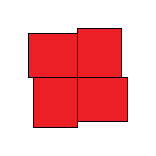
\begin{tikzpicture}[scale=0.07]
            \filldraw[fill=custom-red, draw=black] (11,10) rectangle (19,19);
\filldraw[fill=custom-red, draw=black] (10,19) rectangle (19,27);
\filldraw[fill=custom-red, draw=black] (19,11) rectangle (28,19);
\filldraw[fill=custom-red, draw=black] (19,19) rectangle (27,28);
        \end{tikzpicture}
    \end{subfigure}
    ~
    \begin{subfigure}[b]{0.14\textwidth}
        \centering
        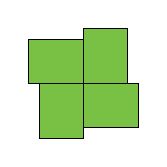
\begin{tikzpicture}[scale=0.07]
            \filldraw[fill=custom-green, draw=black] (11,9) rectangle (19,19);
\filldraw[fill=custom-green, draw=black] (9,19) rectangle (19,27);
\filldraw[fill=custom-green, draw=black] (19,11) rectangle (29,19);
\filldraw[fill=custom-green, draw=black] (19,19) rectangle (27,29);
        \end{tikzpicture}
    \end{subfigure}
    ~
    \begin{subfigure}[b]{0.14\textwidth}
        \centering
        
\begin{tikzpicture}[scale=0.07]
            \filldraw[fill=custom-blue, draw=black] (11,7) rectangle (19,19);
\filldraw[fill=custom-blue, draw=black] (7,19) rectangle (19,27);
\filldraw[fill=custom-blue, draw=black] (19,11) rectangle (31,19);
\filldraw[fill=custom-blue, draw=black] (19,19) rectangle (27,31);
        \end{tikzpicture}
    \end{subfigure}
    ~
    \begin{subfigure}[b]{0.14\textwidth}
        \centering
        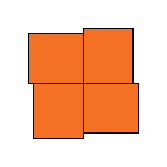
\begin{tikzpicture}[scale=0.07]
            \filldraw[fill=custom-orange, draw=black] (10,9) rectangle (19,19);
\filldraw[fill=custom-orange, draw=black] (9,19) rectangle (19,28);
\filldraw[fill=custom-orange, draw=black] (19,10) rectangle (29,19);
\filldraw[fill=custom-orange, draw=black] (19,19) rectangle (28,29);
        \end{tikzpicture}
    \end{subfigure}
    ~
    \begin{subfigure}[b]{0.14\textwidth}
        \centering
        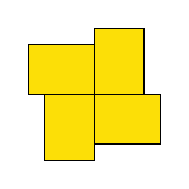
\begin{tikzpicture}[scale=0.07]
            \filldraw[fill=custom-yellow, draw=black] (10,7) rectangle (19,19);
\filldraw[fill=custom-yellow, draw=black] (7,19) rectangle (19,28);
\filldraw[fill=custom-yellow, draw=black] (19,10) rectangle (31,19);
\filldraw[fill=custom-yellow, draw=black] (19,19) rectangle (28,31);
        \end{tikzpicture}
    \end{subfigure}
    ~
    \begin{subfigure}[b]{0.14\textwidth}
        \centering
        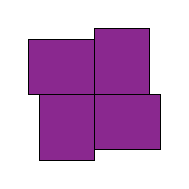
\begin{tikzpicture}[scale=0.07]
            \filldraw[fill=custom-violet, draw=black] (9,7) rectangle (19,19);
\filldraw[fill=custom-violet, draw=black] (7,19) rectangle (19,29);
\filldraw[fill=custom-violet, draw=black] (19,9) rectangle (31,19);
\filldraw[fill=custom-violet, draw=black] (19,19) rectangle (29,31);
        \end{tikzpicture}
    \end{subfigure}
    \caption{Square kernels in the four-dimensional case which have only 2 distinct symmetries.}
    \label{fig:4d-square-self-two-symmetric-kernels}
\end{figure}

Such a kernel consists of 4 of the same type of rectangle and the only distinct symmetry is obtained by a reflection. There are 18 kernels, which have only 4 distinct symmetries and these can be seen in \cref{fig:4d-square-self-four-symmetric-kernels}.

\begin{figure}[ht]
    \centering
    \begin{subfigure}[b]{0.14\textwidth}
        \centering
        
\begin{tikzpicture}[scale=0.07]
            \filldraw[fill=custom-red, draw=black] (11,10) rectangle (19,19);
\filldraw[fill=custom-orange, draw=black] (10,19) rectangle (19,29);
\filldraw[fill=custom-orange, draw=black] (19,9) rectangle (28,19);
\filldraw[fill=custom-red, draw=black] (19,19) rectangle (27,28);
        \end{tikzpicture}
    \end{subfigure}
    ~
    \begin{subfigure}[b]{0.14\textwidth}
        \centering
        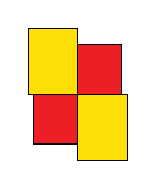
\begin{tikzpicture}[scale=0.07]
            \filldraw[fill=custom-red, draw=black] (11,10) rectangle (19,19);
\filldraw[fill=custom-yellow, draw=black] (10,19) rectangle (19,31);
\filldraw[fill=custom-yellow, draw=black] (19,7) rectangle (28,19);
\filldraw[fill=custom-red, draw=black] (19,19) rectangle (27,28);
        \end{tikzpicture}
    \end{subfigure}
    ~
    \begin{subfigure}[b]{0.14\textwidth}
        \centering
        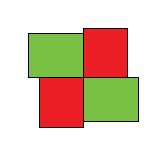
\begin{tikzpicture}[scale=0.07]
            \filldraw[fill=custom-red, draw=black] (11,10) rectangle (19,19);
\filldraw[fill=custom-green, draw=black] (9,19) rectangle (19,27);
\filldraw[fill=custom-green, draw=black] (19,11) rectangle (29,19);
\filldraw[fill=custom-red, draw=black] (19,19) rectangle (27,28);
        \end{tikzpicture}
    \end{subfigure}
    ~
    \begin{subfigure}[b]{0.14\textwidth}
        \centering
        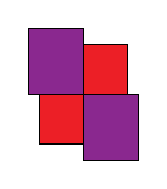
\begin{tikzpicture}[scale=0.07]
            \filldraw[fill=custom-red, draw=black] (11,10) rectangle (19,19);
\filldraw[fill=custom-violet, draw=black] (9,19) rectangle (19,31);
\filldraw[fill=custom-violet, draw=black] (19,7) rectangle (29,19);
\filldraw[fill=custom-red, draw=black] (19,19) rectangle (27,28);
        \end{tikzpicture}
    \end{subfigure}
    ~
    \begin{subfigure}[b]{0.14\textwidth}
        \centering
        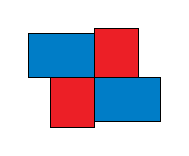
\begin{tikzpicture}[scale=0.07]
            \filldraw[fill=custom-red, draw=black] (11,10) rectangle (19,19);
\filldraw[fill=custom-blue, draw=black] (7,19) rectangle (19,27);
\filldraw[fill=custom-blue, draw=black] (19,11) rectangle (31,19);
\filldraw[fill=custom-red, draw=black] (19,19) rectangle (27,28);
        \end{tikzpicture}
    \end{subfigure}
    ~
    \begin{subfigure}[b]{0.14\textwidth}
        \centering
        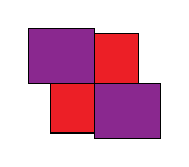
\begin{tikzpicture}[scale=0.07]
            \filldraw[fill=custom-red, draw=black] (11,10) rectangle (19,19);
\filldraw[fill=custom-violet, draw=black] (7,19) rectangle (19,29);
\filldraw[fill=custom-violet, draw=black] (19,9) rectangle (31,19);
\filldraw[fill=custom-red, draw=black] (19,19) rectangle (27,28);
        \end{tikzpicture}
    \end{subfigure}
    \par\bigskip
    \begin{subfigure}[b]{0.14\textwidth}
        \centering
        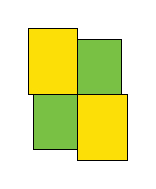
\begin{tikzpicture}[scale=0.07]
            \filldraw[fill=custom-green, draw=black] (11,9) rectangle (19,19);
\filldraw[fill=custom-yellow, draw=black] (10,19) rectangle (19,31);
\filldraw[fill=custom-yellow, draw=black] (19,7) rectangle (28,19);
\filldraw[fill=custom-green, draw=black] (19,19) rectangle (27,29);
        \end{tikzpicture}
    \end{subfigure}
    ~
    \begin{subfigure}[b]{0.14\textwidth}
        \centering
        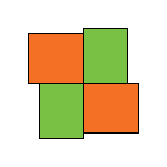
\begin{tikzpicture}[scale=0.07]
            \filldraw[fill=custom-green, draw=black] (11,9) rectangle (19,19);
\filldraw[fill=custom-orange, draw=black] (9,19) rectangle (19,28);
\filldraw[fill=custom-orange, draw=black] (19,10) rectangle (29,19);
\filldraw[fill=custom-green, draw=black] (19,19) rectangle (27,29);
        \end{tikzpicture}
    \end{subfigure}
    ~
    \begin{subfigure}[b]{0.14\textwidth}
        \centering
        \begin{tikzpicture}[scale=0.07]
            \filldraw[fill=custom-green, draw=black] (11,9) rectangle (19,19);
\filldraw[fill=custom-violet, draw=black] (9,19) rectangle (19,31);
\filldraw[fill=custom-violet, draw=black] (19,7) rectangle (29,19);
\filldraw[fill=custom-green, draw=black] (19,19) rectangle (27,29);
        \end{tikzpicture}
    \end{subfigure}
    ~
    \begin{subfigure}[b]{0.14\textwidth}
        \centering
        \begin{tikzpicture}[scale=0.07]
            \filldraw[fill=custom-green, draw=black] (11,9) rectangle (19,19);
\filldraw[fill=custom-blue, draw=black] (7,19) rectangle (19,27);
\filldraw[fill=custom-blue, draw=black] (19,11) rectangle (31,19);
\filldraw[fill=custom-green, draw=black] (19,19) rectangle (27,29);
        \end{tikzpicture}
    \end{subfigure}
    ~
    \begin{subfigure}[b]{0.14\textwidth}
        \centering
        \begin{tikzpicture}[scale=0.07]
            \filldraw[fill=custom-green, draw=black] (11,9) rectangle (19,19);
\filldraw[fill=custom-yellow, draw=black] (7,19) rectangle (19,28);
\filldraw[fill=custom-yellow, draw=black] (19,10) rectangle (31,19);
\filldraw[fill=custom-green, draw=black] (19,19) rectangle (27,29);
        \end{tikzpicture}
    \end{subfigure}
    ~
    \begin{subfigure}[b]{0.14\textwidth}
        \centering
        \begin{tikzpicture}[scale=0.07]
            \filldraw[fill=custom-blue, draw=black] (11,7) rectangle (19,19);
\filldraw[fill=custom-orange, draw=black] (10,19) rectangle (19,29);
\filldraw[fill=custom-orange, draw=black] (19,9) rectangle (28,19);
\filldraw[fill=custom-blue, draw=black] (19,19) rectangle (27,31);
        \end{tikzpicture}
    \end{subfigure}
    \par\bigskip
    \begin{subfigure}[b]{0.14\textwidth}
        \centering
        \begin{tikzpicture}[scale=0.07]
            \filldraw[fill=custom-blue, draw=black] (11,7) rectangle (19,19);
\filldraw[fill=custom-orange, draw=black] (9,19) rectangle (19,28);
\filldraw[fill=custom-orange, draw=black] (19,10) rectangle (29,19);
\filldraw[fill=custom-blue, draw=black] (19,19) rectangle (27,31);
        \end{tikzpicture}
    \end{subfigure}
    ~
    \begin{subfigure}[b]{0.14\textwidth}
        \centering
        \begin{tikzpicture}[scale=0.07]
            \filldraw[fill=custom-blue, draw=black] (11,7) rectangle (19,19);
\filldraw[fill=custom-yellow, draw=black] (7,19) rectangle (19,28);
\filldraw[fill=custom-yellow, draw=black] (19,10) rectangle (31,19);
\filldraw[fill=custom-blue, draw=black] (19,19) rectangle (27,31);
        \end{tikzpicture}
    \end{subfigure}
    ~
    \begin{subfigure}[b]{0.14\textwidth}
        \centering
        \begin{tikzpicture}[scale=0.07]
            \filldraw[fill=custom-blue, draw=black] (11,7) rectangle (19,19);
\filldraw[fill=custom-violet, draw=black] (7,19) rectangle (19,29);
\filldraw[fill=custom-violet, draw=black] (19,9) rectangle (31,19);
\filldraw[fill=custom-blue, draw=black] (19,19) rectangle (27,31);
        \end{tikzpicture}
    \end{subfigure}
    ~
    \begin{subfigure}[b]{0.14\textwidth}
        \centering
        \begin{tikzpicture}[scale=0.07]
            \filldraw[fill=custom-orange, draw=black] (10,9) rectangle (19,19);
\filldraw[fill=custom-violet, draw=black] (9,19) rectangle (19,31);
\filldraw[fill=custom-violet, draw=black] (19,7) rectangle (29,19);
\filldraw[fill=custom-orange, draw=black] (19,19) rectangle (28,29);
        \end{tikzpicture}
    \end{subfigure}
    ~
    \begin{subfigure}[b]{0.14\textwidth}
        \centering
        \begin{tikzpicture}[scale=0.07]
            \filldraw[fill=custom-orange, draw=black] (10,9) rectangle (19,19);
\filldraw[fill=custom-yellow, draw=black] (7,19) rectangle (19,28);
\filldraw[fill=custom-yellow, draw=black] (19,10) rectangle (31,19);
\filldraw[fill=custom-orange, draw=black] (19,19) rectangle (28,29);
        \end{tikzpicture}
    \end{subfigure}
    ~
    \begin{subfigure}[b]{0.14\textwidth}
        \centering
        \begin{tikzpicture}[scale=0.07]
            \filldraw[fill=custom-yellow, draw=black] (10,7) rectangle (19,19);
\filldraw[fill=custom-violet, draw=black] (7,19) rectangle (19,29);
\filldraw[fill=custom-violet, draw=black] (19,9) rectangle (31,19);
\filldraw[fill=custom-yellow, draw=black] (19,19) rectangle (28,31);
        \end{tikzpicture}
    \end{subfigure}
    \caption{Square kernels in the four-dimensional case which have only 4 distinct symmetries.}
    \label{fig:4d-square-self-four-symmetric-kernels}
\end{figure}

Such a kernel consists of two pairs of rectangles and the only distinct symmetries are obtained by a reflection and/or a rotation by $\pi/2$. Finally, there are 810 kernels with the ordinary 8 distinct symmetries. Hence, there are exactly 834 unique square kernels and this corresponds to the number above since
\[
810 \cdot 8 + 18 \cdot 4 + 6 \cdot 2 = 6\,564.
\]
Notice that we will have to discard symmetries after determining all completions of a kernel with coinciding symmetries. With this in mind, we have found that there are $6\,406\,310$ unique squares satisfying the Line criterion \labelcref{criterion:line-criterion} and without overlapping bricks for any dimension tuple found in \cref{ex:4d-rdts}.
\end{observation}

\subsection{Combining two-dimensional packings}
It would seem that better branch pruning is needed to find universal packings in the four-dimensional case. One way of obtaining this is to find more criteria. However, they are hard to come by, especially when we do not have a four-dimensional universal packing to examine. Such a packing could help us to come up with conjectures and provide counterexamples. This sparked the idea to follow the constructive proof of \cref{thm:multiplication-of-packings} in order to obtain a four-dimensional packing.

\begin{observation}\label[observation]{obs:combined-4d}
We have combined two-dimensional packings into a four-di\-men\-sional one by following the proof of \cref{thm:multiplication-of-packings}. As the two-dimensional packing we have used the one from \cref{fig:universal-packing-2d}, which is the only unique universal packing for $n = 2$. Using a computer program, we have repeatedly used this solution to pack the groups of hyperrectangles in the proof of \cref{thm:multiplication-of-packings}. This resulted in a four-dimensional universal packing, which is visualized in \cref{fig:4d-universal-packing}.

This technique enables us to obtain several universal packings, because at each step of the proof, we have a choice of how we solve a group. Here we can use any of the two symmetries of the packing in \cref{fig:universal-packing-2d}.
\end{observation}

\begin{remark}
Strictly speaking, we never prove that combining Hoffman packings following the proof of \cref{thm:multiplication-of-packings} will actually result in a Hoffman packing. We leave this for others to formalize and prove thoroughly. We speculate that they might also be able to prove that such a combination preserves stability under permutations to some extend.
\end{remark}

\begin{figure}[ht]
    \centering
    \begin{subfigure}[b]{0.47\textwidth}
        \centering
        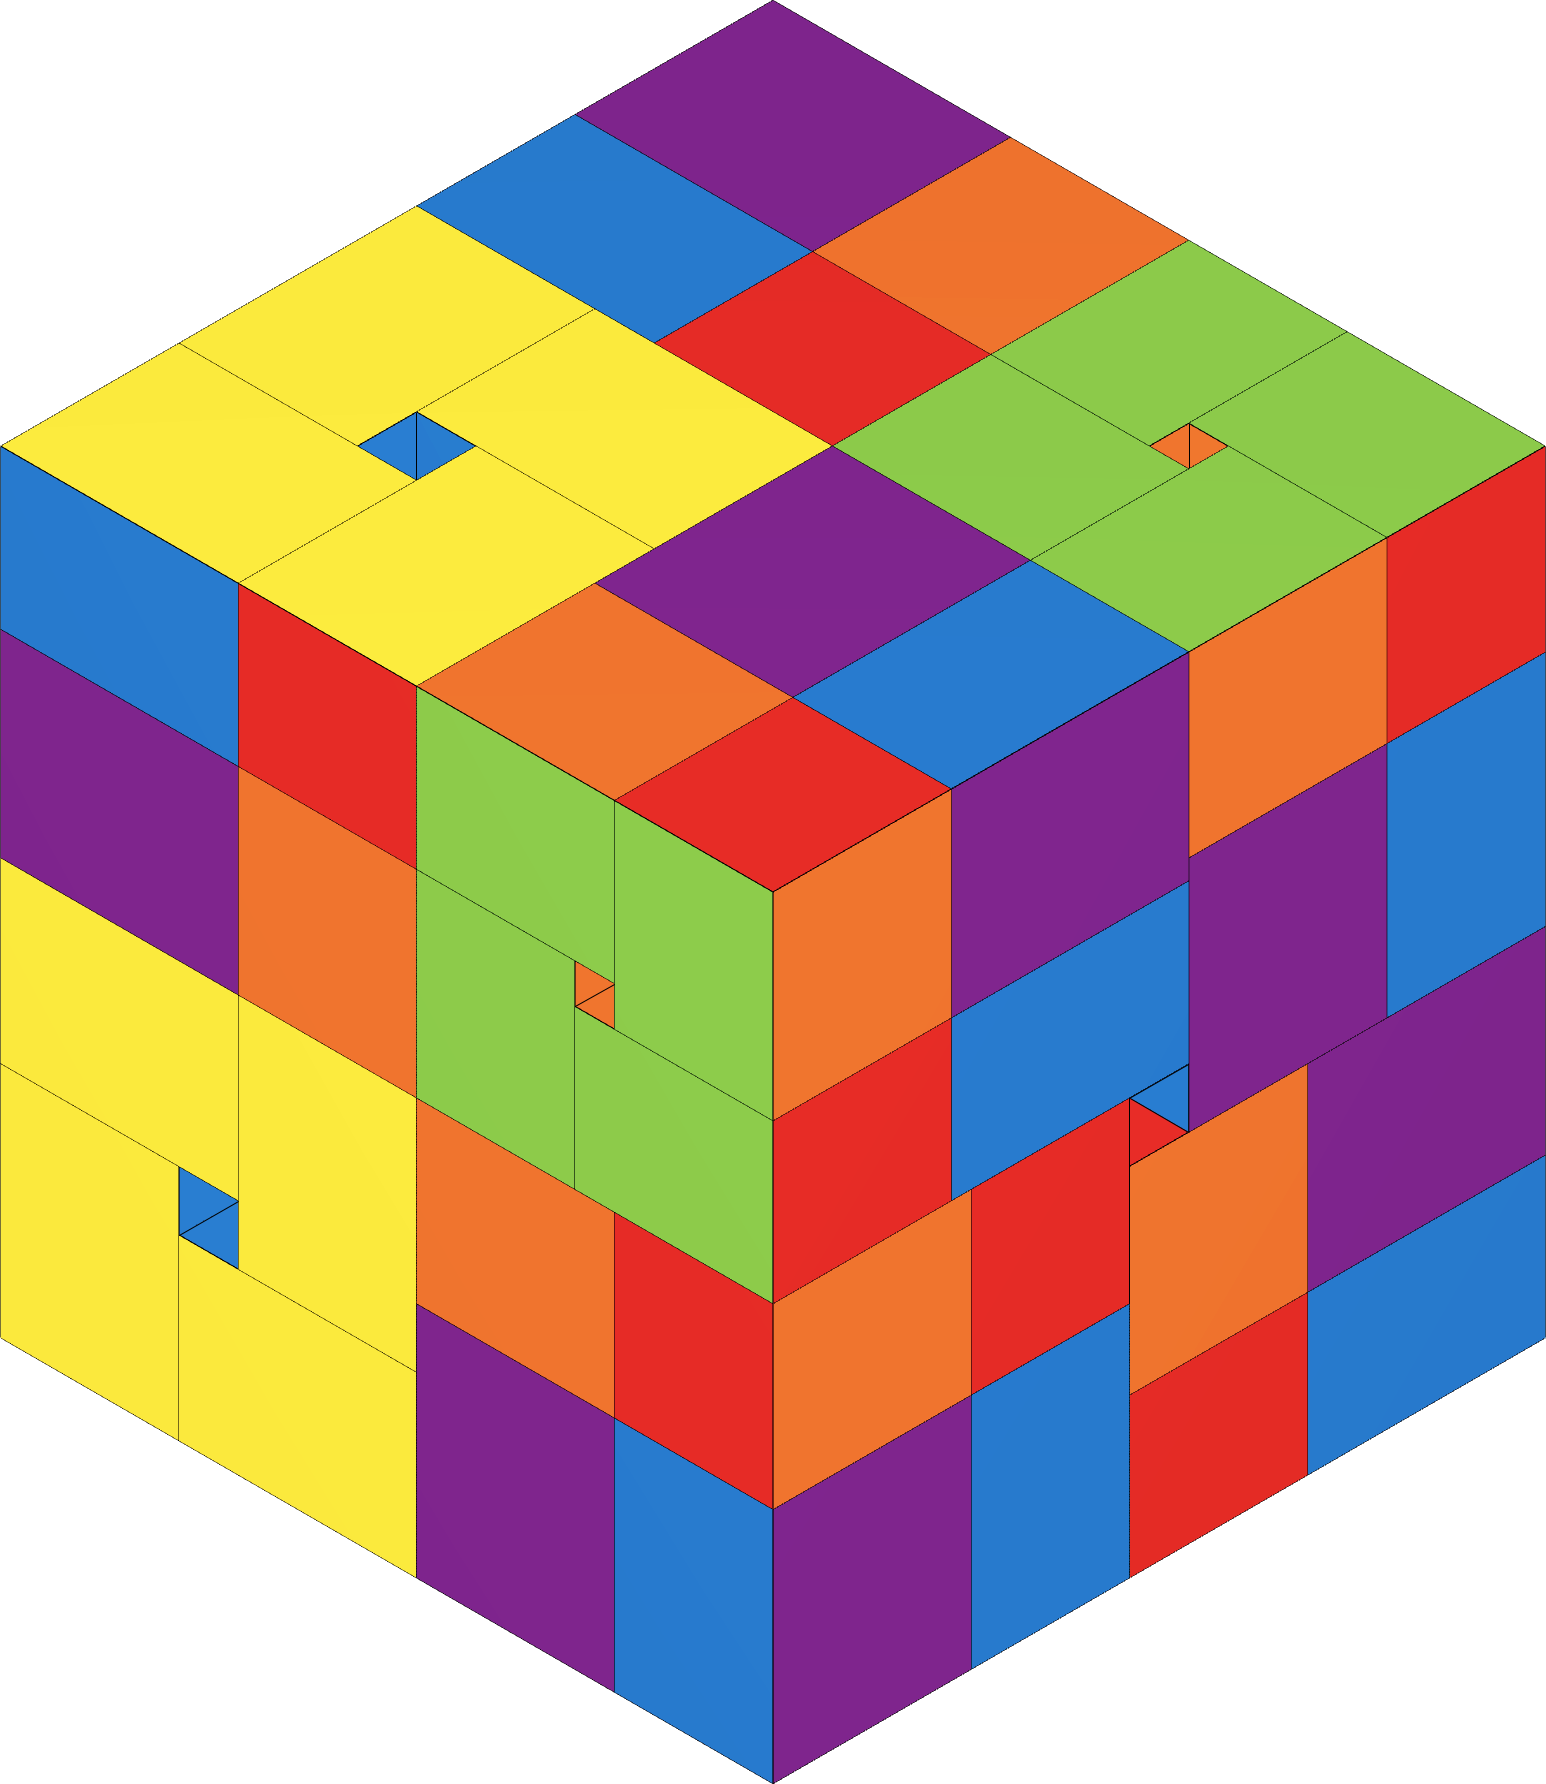
\includegraphics[scale=0.18]{graphics/4d-universal-cube-1.png}
        \caption*{$x = 1$.}
    \end{subfigure}
    ~
    \begin{subfigure}[b]{0.47\textwidth}
        \centering
        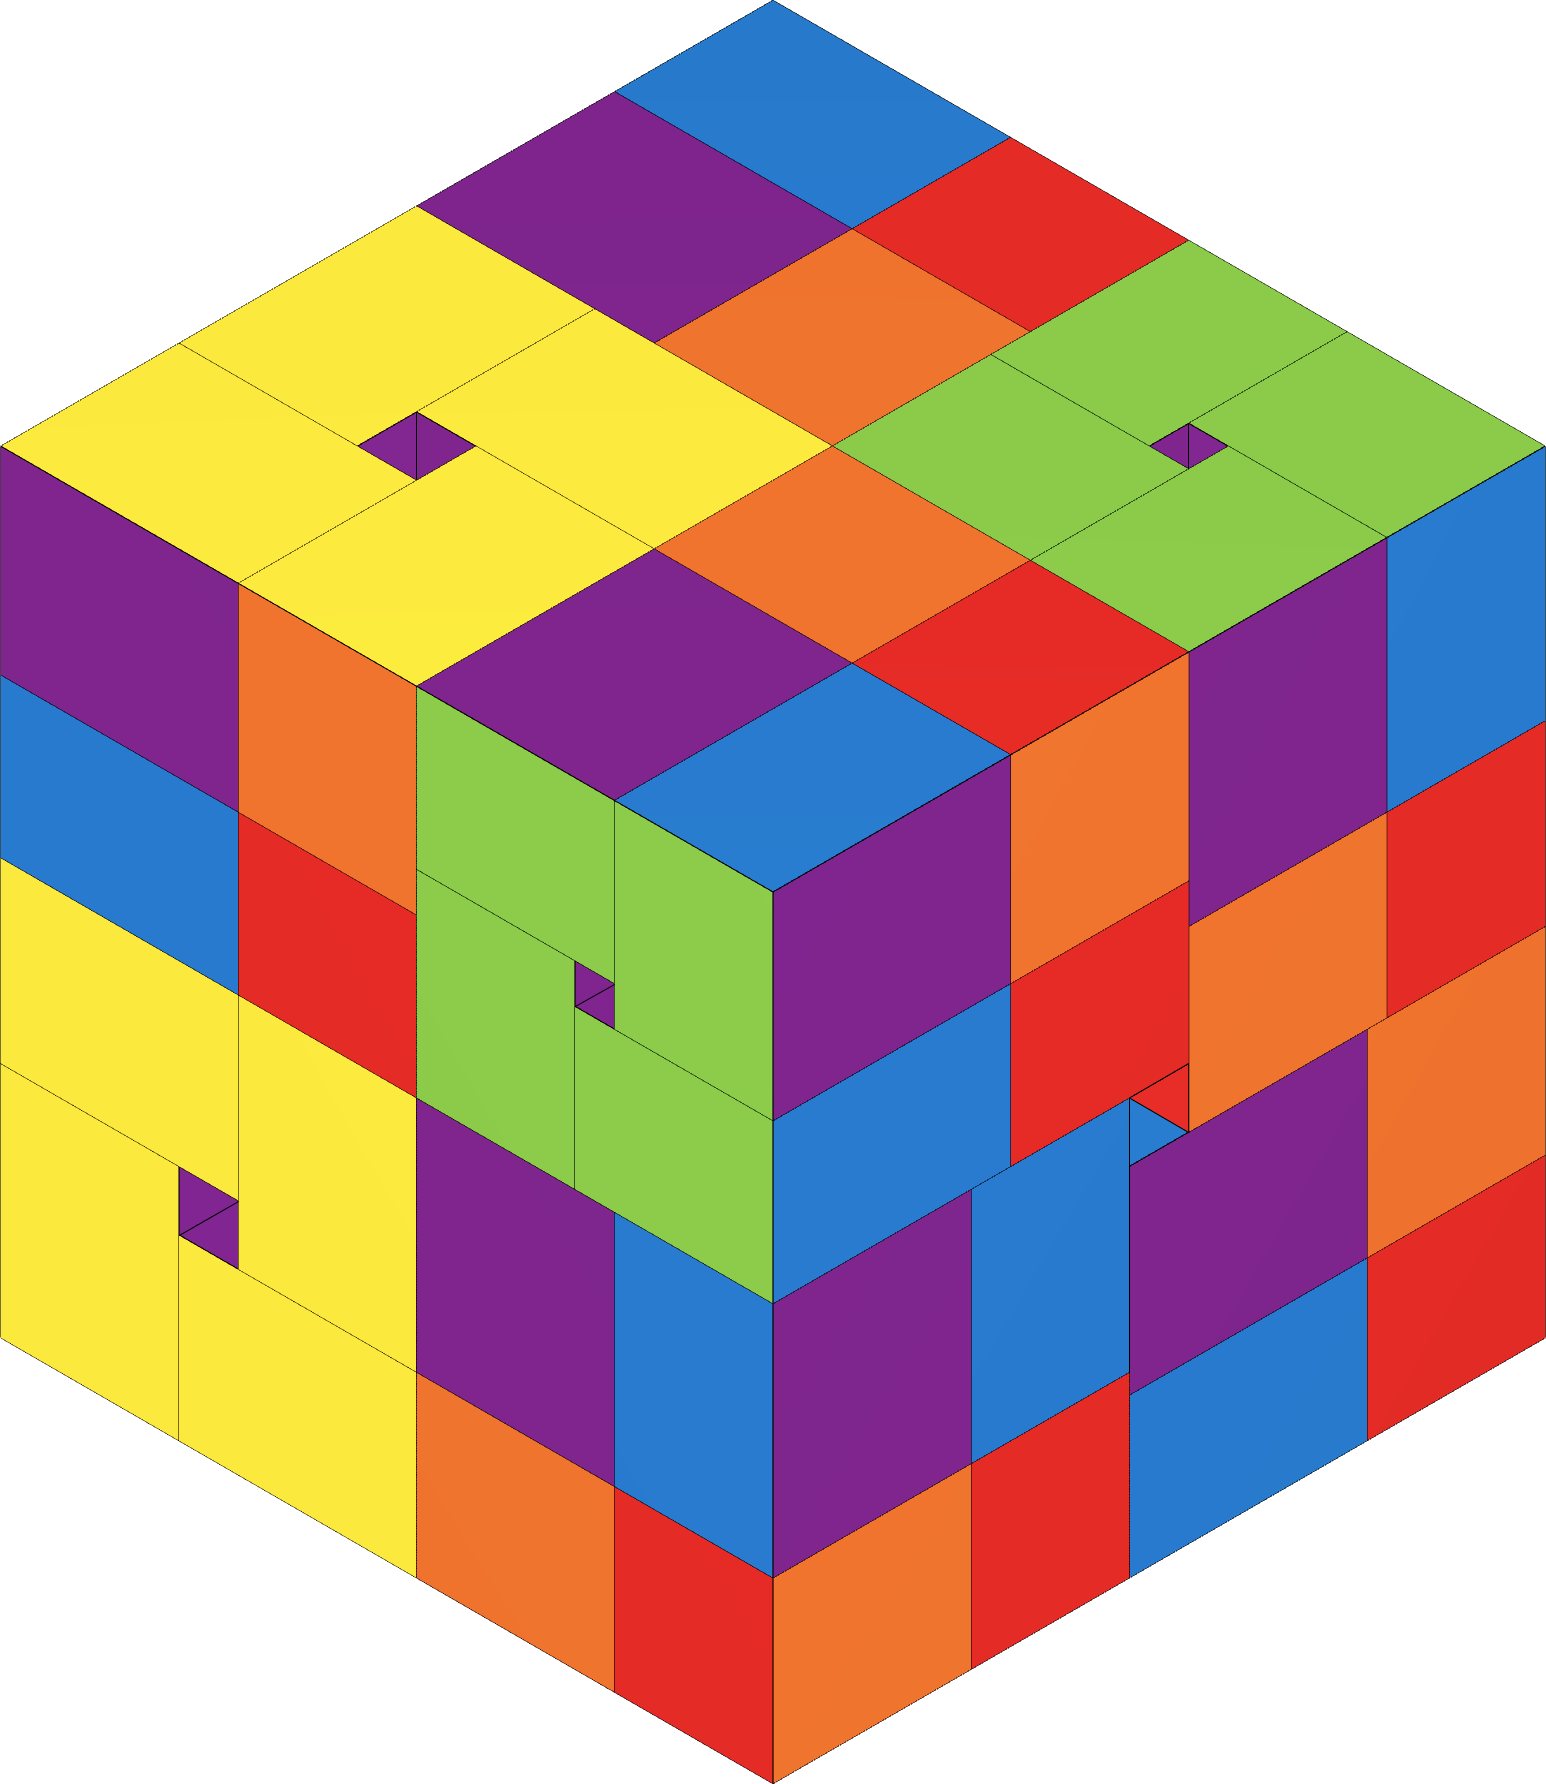
\includegraphics[scale=0.18]{graphics/4d-universal-cube-2.png}
        \caption*{$x = 2$.}
    \end{subfigure}
    \par\bigskip
    \begin{subfigure}[b]{0.47\textwidth}
        \centering
        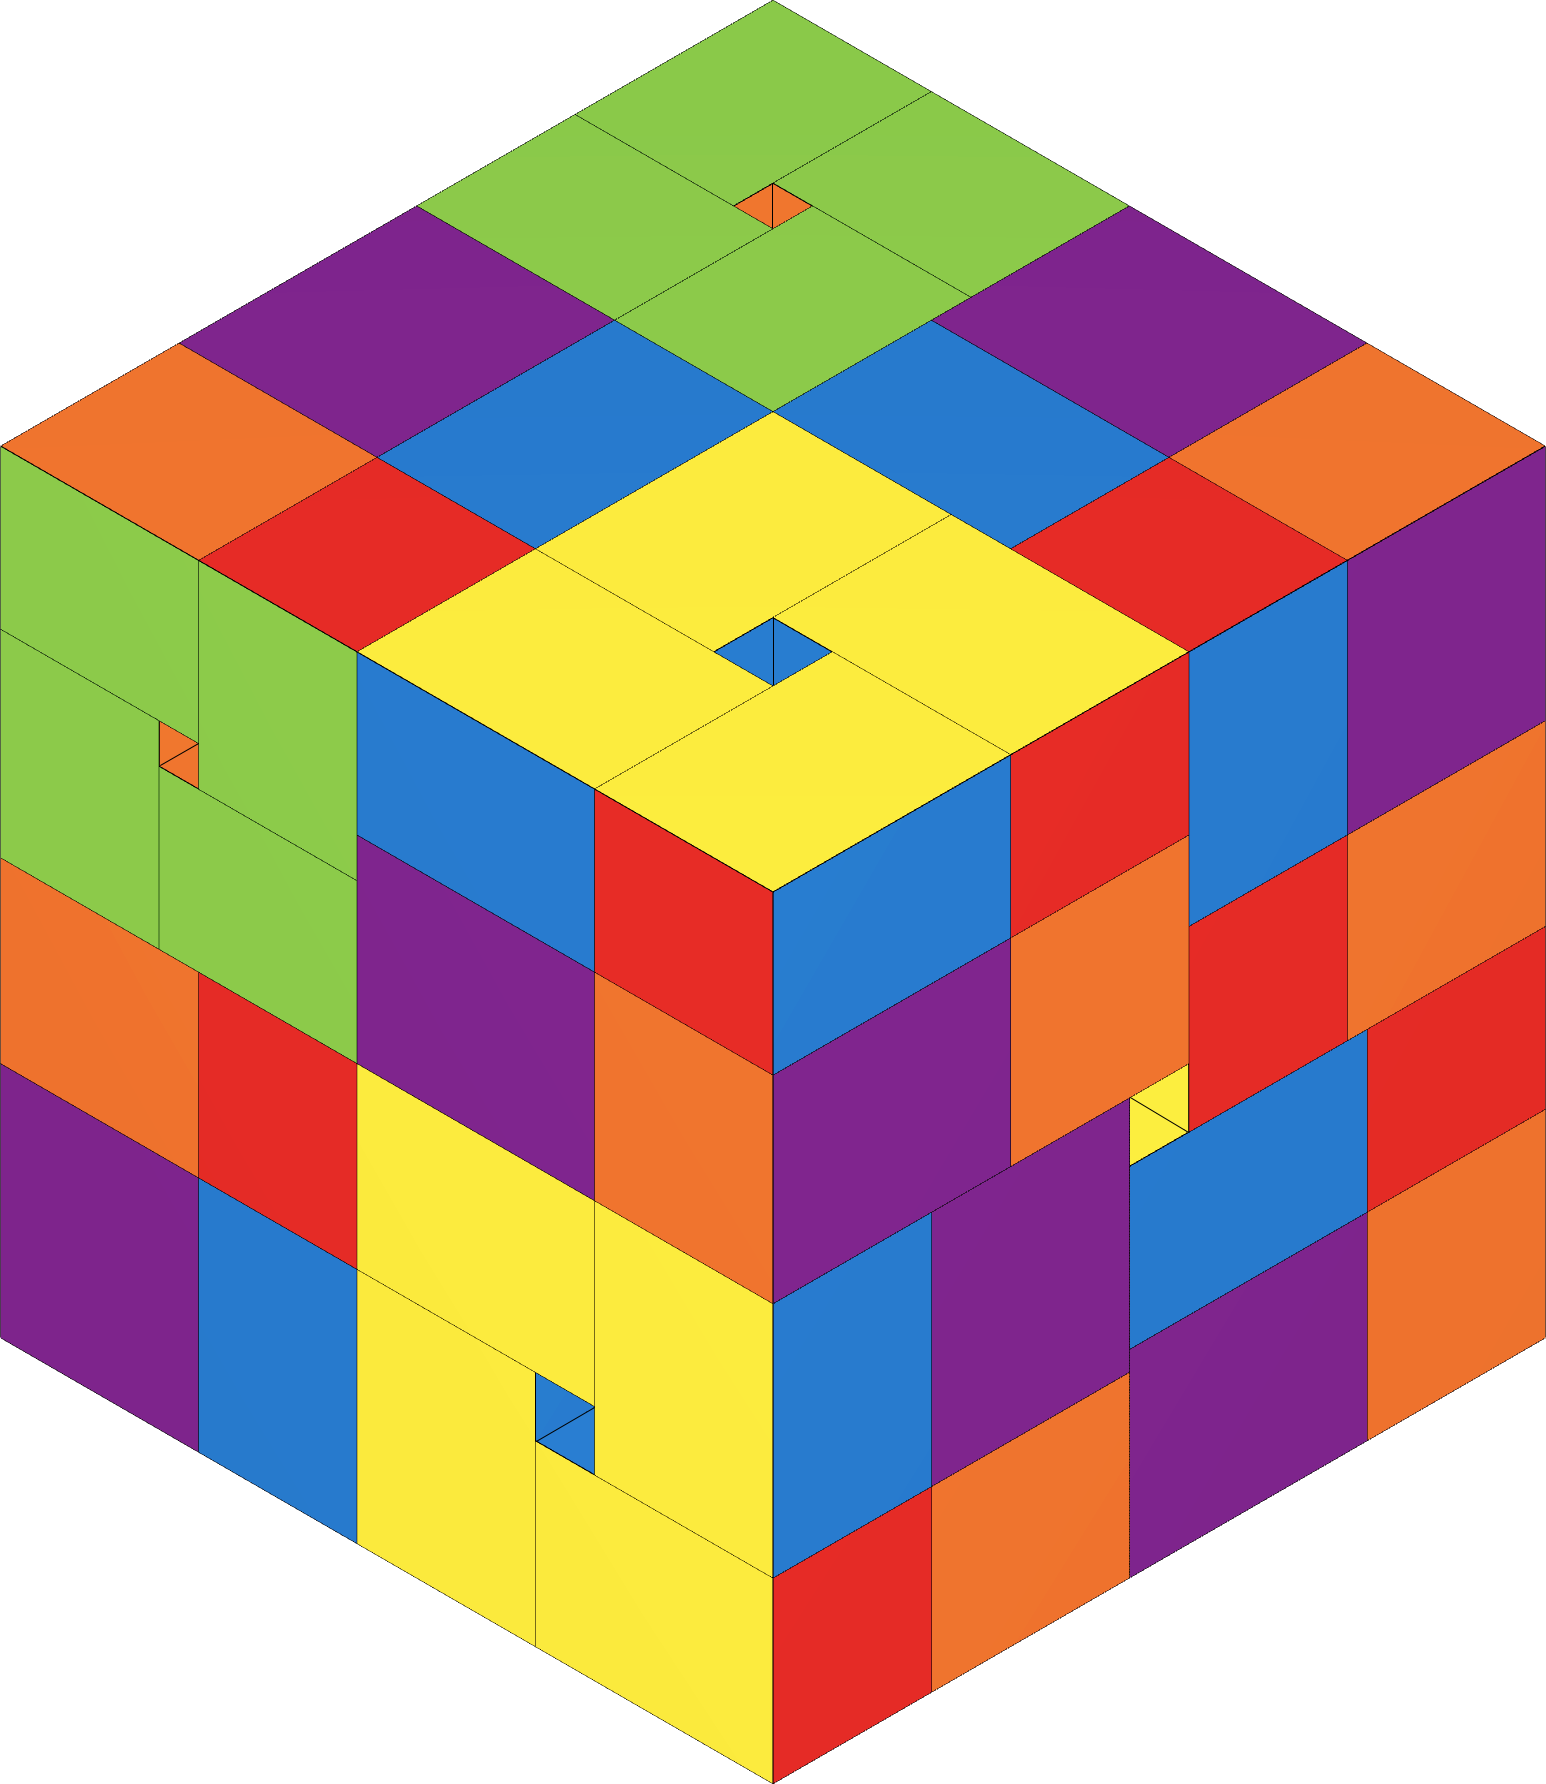
\includegraphics[scale=0.18]{graphics/4d-universal-cube-3.png}
        \caption*{$x = 3$.}
    \end{subfigure}
    ~
    \begin{subfigure}[b]{0.47\textwidth}
        \centering
        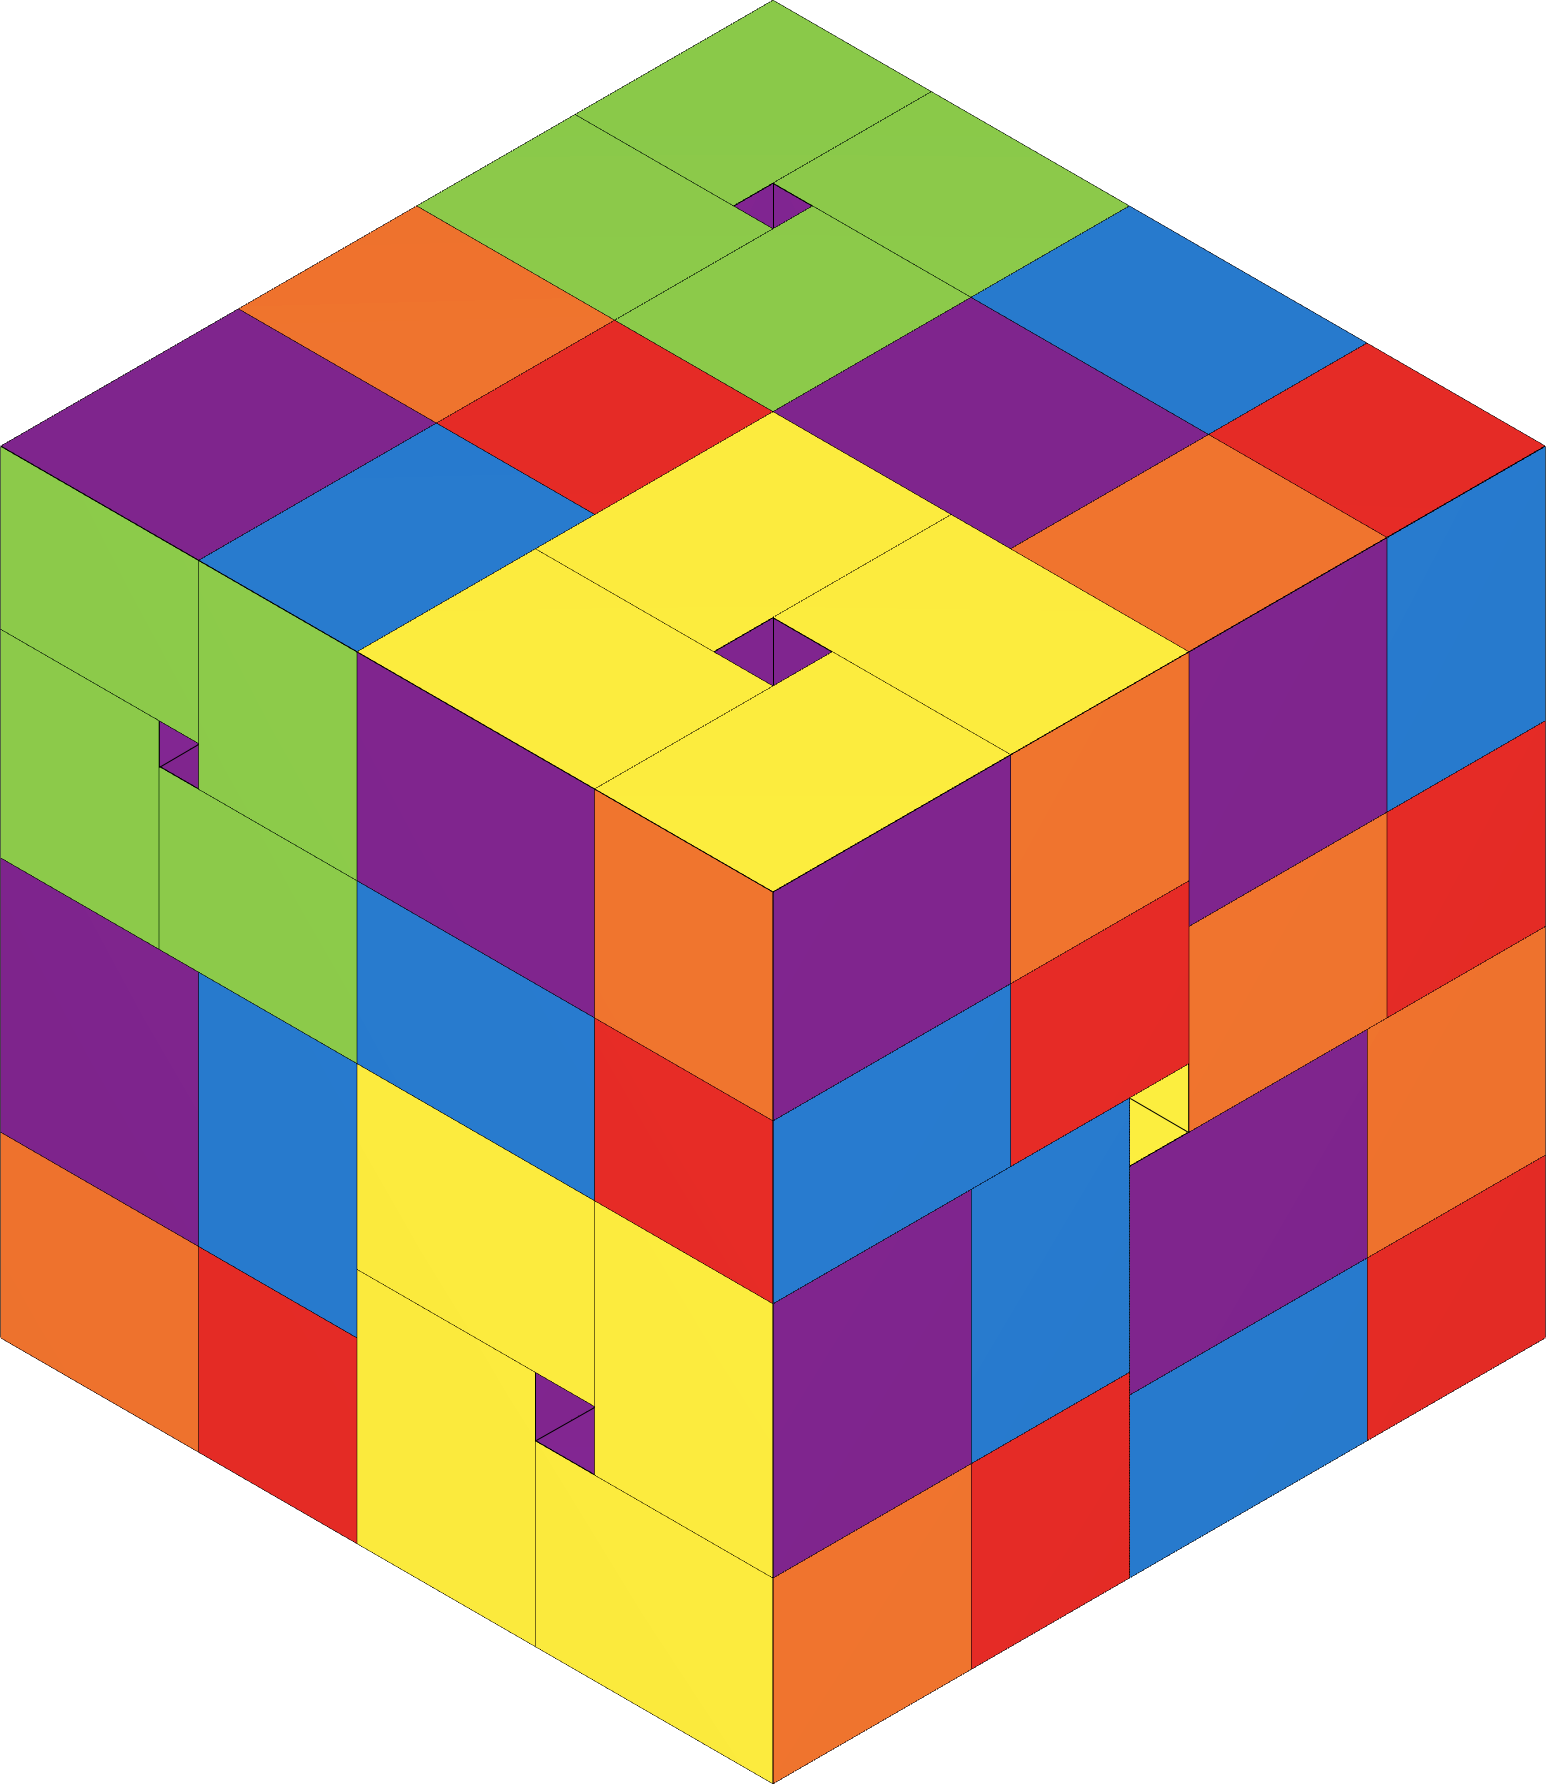
\includegraphics[scale=0.18]{graphics/4d-universal-cube-4.png}
        \caption*{$x = 4$.}
    \end{subfigure}
    \caption{Visualization of the four cubes of a four-dimensional universal packing where the $x$-axis is fixed. The packing has been produced using the dimension tuple $\paren{8, 9, 10, 12}$.}
    \label{fig:4d-universal-packing}
\end{figure}

\noindent These universal packings behave extremely nice.

\begin{observation}
Notice that the two-dimensional packing in \cref{fig:universal-packing-2d} is stable under any permutation from $S_2$. We have examined whether the universal packings constructed in \cref{obs:combined-4d} are stable under permutations from $S_4$. It turns out that they are stable under any permutation from $S_4$. We speculate that this property is inherited through the proof of \cref{thm:multiplication-of-packings}. It is dubious whether all four-dimensional universal packings exhibit this property. It is worth noting that this investigation also resulted in the universal packing from which \cref{fig:4d-square-universal} originates and thus sparked the investigation into a RDTS.
\end{observation}

\subsection{The subgrid criterion}
The four-dimensional universal packings constructed in \cref{obs:combined-4d} provided the inspiration for how to generalize the last major piece of knowledge provided by Hoffman in \cite[p. 221]{Hoffman1981} about the three-dimensional problem. Let $(x_1, x_2, x_3)$ be an increasing dimension tuple with distinct elements. Consider a square of it produced by a three-dimensional universal packing. Such a square contains $3^2 = 9$ rectangles, and Hoffman notes that these $9$ rectangles must comprise exactly 3 $x_1$-by-$x_2$'s, $x_1$-by-$x_3$'s and $x_2$-by-$x_3$'s. This is illustrated in \cref{fig:universal-packing-3d} where each type of rectangle has been given its own color. This observation has proven to be effective at pruning the search tree as seen in \cref{fig:backtracking-3d} and \cref{table:backtracking-3d}. Hence, we have had a great interest in generalizing this observation to higher dimensions in the hope that it will be similarly effective there.

\begin{observation}
The following is the case for any of the universal packings constructed in \cref{obs:combined-4d}. Let $(x_1, x_2, x_3, x_4)$ denote the dimension tuple with distinct elements, which has been used. Consider some cube of $G_4$ and note that it produces a subpacking containing $4^3 = 64$ bricks. These 64 bricks comprise exactly 16 $x_1$-by-$x_2$-by-$x_3$'s, $x_1$-by-$x_2$-by-$x_4$'s, $x_1$-by-$x_3$-by-$x_4$'s and $x_2$-by-$x_3$-by-$x_4$'s.
\end{observation}

\noindent This provides enough information to put forward the following criterion.

\begin{criterion}[Subgrid criterion]\label[criterion]{criterion:subgrid-criterion}\index{Criterion!subgrid}
Suppose $n \geq 2$ and suppose $P\colon G_n \to S_n$. We say that $P$ satisfies the \textit{Subgrid criterion} if any $\paren{n - 1}$-dimensional subgrid $U$ of $G_n$ satisfies the following: Suppose $d = \paren{x_1, x_2, \dotsc, x_n}$ is an increasing dimension tuple with distinct elements and consider the subpacking produced by $P$ restricted to $U$. This subpacking (consisting of $n^{n - 1}$ $\paren{n - 1}$-dimensional hyperrectangles) contains precisely $n^{n - 2}$ hyperrectangles without an extent of $x_i$ for all $i = 1, 2, \dotsc, n$.
\end{criterion}

\noindent Even better, we have been able to prove that this is a necessary condition for being a universal packing.

\begin{proposition}
Suppose $n \geq 2$ and suppose $P\colon G_n \to S_n$ is a universal packing. Then $P$ satisfies the Subgrid criterion \labelcref{criterion:subgrid-criterion}.
\end{proposition}

\begin{proof}
Note that $P$ satisfies the Line criterion \labelcref{criterion:line-criterion} by \cref{prop:universal-packing-has-unique-lines}. Take some $\paren{n - 1}$-dimensional subgrid $U$ of $G_n$ and consider the subpacking produced by $P$ restricted to $U$. There are $(n - 1)n^{n - 2}$ grid lines in $U$, since there are $n^{n - 2}$ grid lines along each of the $n - 1$ different dimensions. Take some $i$ in $\curly{1, 2, \dotsc, n}$. For each of these grid lines there must be precisely one hyperrectangle on it with an extent of $x_i$ along the dimension of the grid line. Hence, there are at least $(n - 1)n^{n - 2}$ hyperrectangles in the subpacking with an extent of $x_i$ along some dimension. Notice that the subpacking consists of $n^{n - 1}$ $\paren{n - 1}$-dimensional hyperrectangles with a total number of $(n - 1)n^{n - 1}$ extends. Since $i$ was chosen arbitrarily, it follows that there must be precisely $(n - 1)n^{n - 2}$ hyperrectangles in the subpacking with an extent of $x_i$ along some dimension. Then the subpacking consists of precisely
\[
n^{n - 1} - (n - 1)n^{n - 2} = n^{n - 2}
\]
$\paren{n - 1}$-dimensional hyperrectangles without an extent of $x_i$. Hence, $P$ satisfies the Subgrid criterion \labelcref{criterion:subgrid-criterion}.
\end{proof}

\begin{example}
Suppose we have a packing produced by a universal packing. In the three-dimensional case we can conclude that there will be $3^{3 - 2} = 3$ of each of the 3 different types of rectangles in each square. In the four-dimensional case we can conclude that there must be $4^{4 - 2} = 16$ of each of the 4 different types of bricks in each cube.
\end{example}

\noindent In \cite{Hoffman1981} Hoffman puts great emphasis on the close relationship between inequalities and packing problems and the Subgrid criterion does also have an interesting interpretation as an inequality.

\begin{corollary}
Suppose $n \geq 2$ and suppose there exists a universal packing $P\colon G_n \to S_n$. Then for any dimension tuple $d = \paren{x_1, x_2, \dotsc, x_n}$ satisfying Hoffman's inequality, we have that
\[
n^{n-2}\paren{\sum_{i=1}^{n}{\frac{1}{x_i}}} \paren{\prod_{i=1}^{n}{x_i} }
\leq \paren{\sum_{i=1}^{n}{x_i}}^{n-1}.
\]
\end{corollary}

\begin{proof}
Take some $\paren{n - 1}$-dimensional subgrid $U$ of $G_n$ and consider the subpacking of $d$ produced by $P$ restricted to $U$. Pick some $j$ in $\curly{1, 2, \dotsc, n}$ and let us determine the combined hypervolume of the hyperrectangles without an extent of $x_j$. By the Subgrid criterion \labelcref{criterion:subgrid-criterion} there are $n^{n - 2}$ of these hyperrectangles yielding a combined hypervolume of
\[
\frac{n^{n - 2}}{x_j}\prod_{i = 1}^{n}{x_i}.
\]
Then the combined hypervolume of all of the hyperrectangles in the subpacking is
\[
n^{n-2}\paren{\sum_{i=1}^{n}{\frac{1}{x_i}}} \paren{\prod_{i=1}^{n}{x_i}}.
\]
Notice that the surrounding $\paren{n - 1}$-dimensional hypercube has an extent of $x_1 + x_2 + \dotsb + x_n$ and hence a hypervolume of $\paren{x_1 + x_2 + \dotsb + x_n}^{n - 1}$. All of the $\paren{n - 1}$-dimensional hyperrectangles are pairwise non-overlapping and contained inside the surrounding $\paren{n - 1}$-dimensional hypercube. Hence, the inequality holds.
\end{proof}

\noindent This is interesting, since if the above inequality does not hold in general, then it might be possible to rule out the existence of a Hoffman packing for certain dimension tuples and perhaps even show that a dimension is not good. However, it turns out that this inequality does in fact hold in general, since it follows quite easily \cite{Martin2017} from Maclaurin's inequality \cite[p. 188]{Cvetkovski2012}. For $n = 4$, Maclaurin's inequality states that
\begin{align}
\frac{x_1 + x_2 + x_3 + x_4}{4}
&\ge \sqrt{\frac{x_1x_2 + x_1x_3 + x_1x_4 + x_2x_3 + x_2x_4 + x_3x_4}{6}}\label{eq:4d-mac-2d}\\
&\ge \sqrt[3]{\frac{x_1x_2x_3 + x_1x_2x_4 + x_1x_3x_4 + x_2x_3x_4}{4}}\label{eq:4d-mac-3d}\\
&\ge \sqrt[4]{x_1x_2x_3x_4}.\label{eq:4d-mac-4d}
\end{align}
for any positive real numbers $x_1, x_2, x_3$ and $x_4$. The inequality given by the left-hand side of \eqref{eq:4d-mac-2d} combined with \eqref{eq:4d-mac-4d} expresses the AM-GM inequality, while the inequality given by the left-hand side of \eqref{eq:4d-mac-2d} combined with \eqref{eq:4d-mac-3d} expresses the inequality treated above for $n = 4$. Inspired by Hoffman's focus on the close relationship between inequalities and packing problems let us see if we can find a connection between \eqref{eq:4d-mac-2d} and the four-dimensional problem. This inequality can be rearranged to
\begin{equation}\label{eq:4d-mac-2d-six-squares}
16\paren{x_1x_2 + x_1x_3 + x_1x_4 + x_2x_3 + x_2x_4 + x_3x_4}
\leq 6\paren{x_1 + x_2 + x_3 + x_4}^2
\end{equation}
or equivalently
\begin{equation}\label{eq:4d-mac-2d-three-squares}
8\paren{x_1x_2 + x_1x_3 + x_1x_4 + x_2x_3 + x_2x_4 + x_3x_4}
\leq 3\paren{x_1 + x_2 + x_3 + x_4}^2,
\end{equation}
and the power of two on the right-hand side motivates us to look for a connection among the squares.

\begin{observation}\label[observation]{obs:4d-n-2-subgrid}
The following is the case for any of the universal packings constructed in \cref{obs:combined-4d}. Let $(x_1, x_2, x_3, x_4)$ denote the dimension tuple with distinct elements, which has been used. Take any 3 pairwise ``orthogonal'' squares and consider the $3 \cdot 4^2 = 48$ rectangles in them. These 48 rectangles comprise exactly 8 $x_1$-by-$x_2$'s, $x_1$-by-$x_3$'s, $x_1$-by-$x_4$'s, $x_2$-by-$x_3$'s, $x_2$-by-$x_4$'s and $x_3$-by-$x_4$'s. The phenomenon can be observed in \cref{fig:4d-universal-packing} and all the squares of this packing can be found in \cref{appendix-B}. Notice that this implies that ``parallel'' squares have the same number of each type of rectangle.
\end{observation}

\noindent This corresponds precisely to the inequality \eqref{eq:4d-mac-2d-three-squares}. It has not been possible to prove that this is a necessary condition for being a universal packing. Neither has it been possible to come up with a counterexample. Even if this is not the case, a weaker claim might still hold, namely that there are 16 of each type of rectangle in any six pairwise ``orthogonal'' squares. This corresponds to the inequality \eqref{eq:4d-mac-2d-six-squares}.

In order to come up with a counterexample or strengthen the above two hypotheses, we need another way of constructing a four-dimensional universal packing. Since the ordinary backtracking and dynamic programming approaches does not show much promise, we have also tried an alternative approach.

\begin{observation}
Starting from one of the universal packings constructed in \cref{obs:combined-4d}, we removed a number of hyperrectangles and then attempted to use backtracking to complete this partial solution. We could remove up to 94 hyperrectangles without completely derailing the backtracking algorithm. Without terminating after two days it had found $C = 435\,122\,478$ universal packings. A few random samples of these did not provide a counterexample to any of the two hypotheses above. These solutions appear to have the same overall structure as the universal packings from \cref{obs:combined-4d}, but with some of the hyperrectangles swapped around. This is illustrated in \cref{fig:4d-partial-swaps}. Since any unique four-dimensional universal packing has at most $4! \cdot 2^4 = 384$ non-coinciding symmetries by \cref{prop:universal-symmetries} there must be at least $\floor*{C/384} = 1\,133\,131$ unique universal packings in the four-dimensional case.
\end{observation}

\begin{figure}[ht]
    \centering
    \begin{subfigure}[b]{0.220\textwidth}
        \centering
        \begin{tikzpicture}[scale=0.068]
\filldraw[fill=custom-blue, draw=black] (0,0) rectangle (8,12);
\filldraw[fill=custom-red, draw=black] (0,12) rectangle (8,21);
\filldraw[fill=custom-red, draw=black] (0,21) rectangle (9,29);
\filldraw[fill=custom-orange, draw=black] (0,29) rectangle (9,39);
\filldraw[fill=custom-violet, draw=black] (8,0) rectangle (18,12);
\filldraw[fill=custom-orange, draw=black] (8,12) rectangle (18,21);
\filldraw[fill=custom-blue, draw=black] (9,21) rectangle (21,29);
\filldraw[fill=custom-violet, draw=black] (9,29) rectangle (21,39);
\filldraw[fill=custom-blue, draw=black] (18,0) rectangle (30,8);
\filldraw[fill=custom-violet, draw=black] (18,8) rectangle (30,18);
\filldraw[fill=custom-blue, draw=black] (21,18) rectangle (29,30);
\filldraw[fill=custom-red, draw=black] (21,30) rectangle (29,39);
\filldraw[fill=custom-red, draw=black] (30,0) rectangle (39,8);
\filldraw[fill=custom-orange, draw=black] (30,8) rectangle (39,18);
\filldraw[fill=custom-violet, draw=black] (29,18) rectangle (39,30);
\filldraw[fill=custom-orange, draw=black] (29,30) rectangle (39,39);
        \end{tikzpicture}
    \end{subfigure}
    ~
    \begin{subfigure}[b]{0.220\textwidth}
        \centering
        \begin{tikzpicture}[scale=0.068]
\filldraw[fill=custom-blue, draw=black] (0,0) rectangle (8,12);
\filldraw[fill=custom-red, draw=black] (0,12) rectangle (8,21);
\filldraw[fill=custom-blue, draw=black] (0,21) rectangle (12,29);
\filldraw[fill=custom-orange, draw=black] (0,29) rectangle (9,39);
\filldraw[fill=custom-orange, draw=black] (8,0) rectangle (18,9);
\filldraw[fill=custom-violet, draw=black] (8,9) rectangle (18,21);
\filldraw[fill=custom-red, draw=black] (12,21) rectangle (21,29);
\filldraw[fill=custom-violet, draw=black] (9,29) rectangle (21,39);
\filldraw[fill=custom-blue, draw=black] (18,0) rectangle (30,8);
\filldraw[fill=custom-violet, draw=black] (18,8) rectangle (30,18);
\filldraw[fill=custom-blue, draw=black] (21,18) rectangle (29,30);
\filldraw[fill=custom-red, draw=black] (21,30) rectangle (29,39);
\filldraw[fill=custom-red, draw=black] (30,0) rectangle (39,8);
\filldraw[fill=custom-orange, draw=black] (30,8) rectangle (39,18);
\filldraw[fill=custom-violet, draw=black] (29,18) rectangle (39,30);
\filldraw[fill=custom-orange, draw=black] (29,30) rectangle (39,39);
        \end{tikzpicture}
    \end{subfigure}
    ~
    \begin{subfigure}[b]{0.220\textwidth}
        \centering
        \begin{tikzpicture}[scale=0.068]
\filldraw[fill=custom-blue, draw=black] (0,0) rectangle (8,12);
\filldraw[fill=custom-red, draw=black] (0,12) rectangle (8,21);
\filldraw[fill=custom-blue, draw=black] (0,21) rectangle (12,29);
\filldraw[fill=custom-violet, draw=black] (0,29) rectangle (12,39);
\filldraw[fill=custom-orange, draw=black] (8,0) rectangle (18,9);
\filldraw[fill=custom-violet, draw=black] (8,9) rectangle (18,21);
\filldraw[fill=custom-red, draw=black] (12,21) rectangle (21,29);
\filldraw[fill=custom-orange, draw=black] (12,29) rectangle (21,39);
\filldraw[fill=custom-red, draw=black] (18,0) rectangle (27,8);
\filldraw[fill=custom-violet, draw=black] (18,8) rectangle (30,18);
\filldraw[fill=custom-blue, draw=black] (21,18) rectangle (29,30);
\filldraw[fill=custom-red, draw=black] (21,30) rectangle (29,39);
\filldraw[fill=custom-blue, draw=black] (27,0) rectangle (39,8);
\filldraw[fill=custom-orange, draw=black] (30,8) rectangle (39,18);
\filldraw[fill=custom-violet, draw=black] (29,18) rectangle (39,30);
\filldraw[fill=custom-orange, draw=black] (29,30) rectangle (39,39);
        \end{tikzpicture}
    \end{subfigure}
    ~
    \begin{subfigure}[b]{0.220\textwidth}
        \centering
        \begin{tikzpicture}[scale=0.068]
\filldraw[fill=custom-blue, draw=black] (0,0) rectangle (8,12);
\filldraw[fill=custom-red, draw=black] (0,12) rectangle (8,21);
\filldraw[fill=custom-blue, draw=black] (0,21) rectangle (12,29);
\filldraw[fill=custom-orange, draw=black] (0,29) rectangle (9,39);
\filldraw[fill=custom-orange, draw=black] (8,0) rectangle (18,9);
\filldraw[fill=custom-violet, draw=black] (8,9) rectangle (18,21);
\filldraw[fill=custom-red, draw=black] (12,21) rectangle (21,29);
\filldraw[fill=custom-violet, draw=black] (9,29) rectangle (21,39);
\filldraw[fill=custom-red, draw=black] (18,0) rectangle (27,8);
\filldraw[fill=custom-violet, draw=black] (18,8) rectangle (30,18);
\filldraw[fill=custom-blue, draw=black] (21,18) rectangle (29,30);
\filldraw[fill=custom-red, draw=black] (21,30) rectangle (29,39);
\filldraw[fill=custom-blue, draw=black] (27,0) rectangle (39,8);
\filldraw[fill=custom-orange, draw=black] (30,8) rectangle (39,18);
\filldraw[fill=custom-violet, draw=black] (29,18) rectangle (39,30);
\filldraw[fill=custom-orange, draw=black] (29,30) rectangle (39,39);
        \end{tikzpicture}
    \end{subfigure}
    \caption{Example of how completing a partial solution in multiple ways might lead to a swapping of some of the hyperrectangles.}
    \label{fig:4d-partial-swaps}
\end{figure}


\noindent This observation indicates that some regions of the search space might have a particularly high density of solutions and also that there are a \textit{lot} of four-dimensional unique universal packings compared to the three-dimensional case.

\section{Approaching the five-dimensional case}
\noindent Due to time constraints our research into the five-dimensional case has been rather sparse. However, our formalization of the problem and the theoretical framework introduced does enable us to provide a few insights. We begin with a RDTS.

\begin{example}[RDTS for $n = 5$]\label[example]{ex:5d-rdts}
In this case all overlap inequalities have arity $1$, $2$, $3$ or $4$. By \cref{prop:arity-reduction} we only have to consider the overlap inequalities with arity $1$ or $2$. We would like to choose a dimension tuple $\paren{x_1, x_2, x_3, x_4, x_5}$ satisfying Hoffman's inequality and containing distinct elements, since by doing so we can make sure that of the overlap inequalities with arity $1$, such a dimension tuple will only satisfy the trivial ones. Then we only need to consider the overlap inequalities with arity $2$. Next, we follow the same line of thought as in \cref{ex:4d-rdts} where it resulted in a pair of non-trivial overlap inequalities, where at most one could not be satisfied. This resulted in an RDTS with two dimension tuples. Now, we end up with 5 pairs, namely 
\begin{align*}
\paren{A, B}, \paren{B, A}, 
&\paren{B, C}, \paren{C, B},\\
\paren{C, D}, \paren{D, C}, 
&\paren{C, F}, \paren{C, F},\\
\paren{E, F}, & \paren{F, E},
\end{align*}
where
$A = \curly{1, 4}$, 
$B = \curly{2, 3}$, 
$C = \curly{1, 5}$, 
$D = \curly{2, 4}$, 
$E = \curly{2, 5}$
and
$F = \curly{3, 4}$. Hence, any dimension tuple must always satisfy at least five non-trivial overlap inequalities. Intuitively, we are attempting to cover every possible way to linearly order the sums of two distinct terms (without any two sums with different terms being equal) and this is illustrated in \cref{fig:hasse-5d-arity-2}. Then, one might suspect there to be $2^5 = 32$ minimal equivalence classes of dimension tuples, but this is not the case. Some of these overlap inequalities are in fact mutually dependent on one another in an intricate way as illustrated in \cref{fig:5d-decision-tree}.
\begin{figure}[ht]
    \centering
    \begin{tikzpicture}[scale=0.70]
        \node(d1) at (-8, 0) {$[d_1]$};
        \node(d2) at (-6, 0) {$[d_2]$};
        \node(d3) at (-5, 0) {$[d_3]$};
        \node(d4) at (-3, 0) {$[d_4]$};
        \node(d5) at (-2, 0) {$[d_5]$};
        
        \node(d6) at (-1, 0) {$[d_6]$};
        \node(d7) at (1, 0) {$[d_7]$};
        
        \node(d8) at (2, 0) {$[d_8]$};
        \node(d9) at (4, 0) {$[d_9]$};
        \node(d10) at (5, 0) {$[d_{10}]$};
        \node(d11) at (7, 0) {$[d_{11}]$};
        \node(d12) at (8, 0) {$[d_{12}]$};
        % (E, F)
        \node(ef1) at (-7, 2) {$\paren{E, F}$};
        \node(ef2) at (-4, 2) {$\paren{E, F}$};
        \node(ef3) at (-2, 2) {$\paren{E, F}$};
        \node(ef4) at (0, 2) {$\paren{E, F}$};
        \node(ef5) at (3, 2) {$\paren{E, F}$};
        \node(ef6) at (6, 2) {$\paren{E, F}$};
        \node(ef7) at (8, 2) {$\paren{E, F}$};
        % (C, F)
        \node(cf1) at (-6, 4) {$\paren{C, F}$};
        \node(cf2) at (-3, 4) {$\paren{C, F}$};
        \node(cf3) at (0, 4) {$\paren{C, F}$};
        \node(cf4) at (3, 4) {$\paren{C, F}$};
        \node(cf5) at (6, 4) {$\paren{C, F}$};
        % (C, D)
        \node(cd1) at (-4, 6) {$\paren{C, D}$};
        \node(cd2) at (0, 6) {$\paren{C, D}$};
        \node(cd3) at (4, 6) {$\paren{C, D}$};
        % (B, C)
        \node(bc1) at (-2, 8) {$\paren{B, C}$};
        \node(bc2) at (2, 8) {$\paren{B, C}$};
        % (A, B)
        \node(ab) at (0, 10) {$\paren{A, B}$};
        
        % Layer 0-2
        \draw (ef1) -- (d1) node [midway, left] {$<$};
        \draw (ef1) -- (d2) node [midway, right] {$>$};
        \draw (ef2) -- (d3) node [midway, left] {$<$};
        \draw (ef2) -- (d4) node [midway, right] {$>$};
        \draw (ef3) -- (d5) node [midway, right] {$>$};
        
        \draw (ef4) -- (d6) node [midway, left] {$<$};
        \draw (ef4) -- (d7) node [midway, right] {$>$};
        
        \draw (ef5) -- (d8) node [midway, left] {$<$};
        \draw (ef5) -- (d9) node [midway, right] {$>$};
        \draw (ef6) -- (d10) node [midway, left] {$<$};
        \draw (ef6) -- (d11) node [midway, right] {$>$};
        \draw (ef7) -- (d12) node [midway, right] {$>$};
        
        % Layer 2-4
        \draw (cf1) -- (ef1) node [midway, left] {$<$};
        
        \draw (cf2) -- (ef2) node [midway, left] {$<$};
        \draw (cf2) -- (ef3) node [midway, right] {$>$};
        
        \draw (cf3) -- (ef4) node [midway, left] {$<$};
        
        \draw (cf4) -- (ef5) node [midway, left] {$<$};

        \draw (cf5) -- (ef6) node [midway, left] {$<$};
        \draw (cf5) -- (ef7) node [midway, right] {$>$};
        
        % Layer 4-6
        \draw (cd1) -- (cf1) node [midway, left] {$<$};
        \draw (cd1) -- (cf2) node [midway, right] {$>$};
        
        \draw (cd2) -- (cf3) node [midway, left] {$<$};
        
        \draw (cd3) -- (cf4) node [midway, left] {$<$};
        \draw (cd3) -- (cf5) node [midway, right] {$>$};
        
        % Layer 6-8
        \draw (bc1) -- (cd1) node [midway, left] {$<$};
        \draw (bc1) -- (cd2) node [midway, right] {$>$};
        
        \draw (bc2) -- (cd3) node [midway, left] {$<$};
        
        % Layer 8-10
        \draw (ab) -- (bc1) node [midway, left] {$<$};
        \draw (ab) -- (bc2) node [midway, right] {$>$};
    \end{tikzpicture}
    \caption{Decision tree showing how not satisfying certain overlap inequalities affect other overlap inequalities. It is quite helpful to compare this with \cref{fig:hasse-5d-arity-2}.}.
    \label{fig:5d-decision-tree}
\end{figure}
By looking at this decision tree we observe that there are in reality only 12 minimal elements. For each of these we have found a representative satisfying Hoffman's inequality, namely
\[
\begin{aligned}[c]
d_1 &= \paren{28, 31, 34, 36, 38},\\
d_4 &= \paren{20, 22, 24, 25, 28},\\
d_7 &= \paren{24, 28, 29, 30, 32},\\
d_{10} &= \paren{20, 21, 24, 26, 28},
\end{aligned}
\quad
\begin{aligned}[c]
d_2 &= \paren{22, 25, 26, 28, 30},\\
d_5 &= \paren{18, 20, 21, 22, 26},\\
d_8 &= \paren{22, 24, 26, 29, 30},\\
d_{11} &= \paren{24, 26, 28, 31, 34},
\end{aligned}
\quad
\begin{aligned}[c]
d_3 &= \paren{26, 28, 32, 33, 36},\\
d_6 &= \paren{22, 25, 27, 28, 29},\\
d_9 &= \paren{26, 29, 30, 34, 36},\\
d_{12} &= \paren{15, 16, 17, 19, 22}.
\end{aligned}
\]
Hence, the set of these 12 dimension tuples constitutes a RDTS for $n = 5$.
\end{example}

\noindent In the four-dimensional case we immediately began counting the number of unique universal packings, since 4 is a good dimension by \cref{thm:multiplication-of-packings}. However, we do not know whether 5 is a good dimension and whether a universal packing exists. Until then we might be better off trying to find a Hoffman packing of each of these 12 dimension tuples individually. Intuitively, they represent the 12 most difficult types of dimension tuples to solve.

\begin{remark}
What about the criteria found to be necessary properties of universal packings? Interestingly, each of the 12 dimension tuples above has properties similar to those of the dimension tuple in \cref{lemma:finding-tuples}, whereby any Hoffman packing of it must necessarily satisfy the Line criterion \labelcref{criterion:line-criterion}. Then the Subgrid criterion \labelcref{criterion:subgrid-criterion} must hold as well. In fact, we suspect that in higher dimensions minimal equivalence classes of dimension tuples will always result in any Hoffman packing necessarily satisfying the Line criterion \labelcref{criterion:line-criterion}.
\end{remark}

\noindent 

\noindent Next, we highlight a few investigations which we deem particularly interesting. They have not been pursued further due to time constraints.

\subsection{Fundamentally different approaches}
It would be interesting to explore the possibilities of making ``local changes'' to a pseudo-packing and use this to gradually reduce the number of overlapping hyperrectangles. One could begin by further exploring the results obtained in \cref{obs:3d-distances}.

It would also be interesting to explore the possibility of reducing a higher dimensional packing to a packing in lower dimensions. This would enable us to create a five-dimensional packing via a reduction of a six-dimensional one obtained via \cref{thm:multiplication-of-packings}. We have made a few failed attempts at reducing a four-dimensional packing to a three-dimensional one. However, others might have better luck.

\subsection{Ties to Maclaurin's inequality}
There are a number of ways to further explore the results obtained in \cref{obs:4d-n-2-subgrid}. First of all, it would be interesting to see if imposing such a criterion significantly speeds up the search process in the four-dimensional case. It is unclear whether this might be the case, since the Subgrid criterion \labelcref{criterion:subgrid-criterion} has proven quite effective at pruning the search tree in the three-dimensional case (as seen in \cref{fig:backtracking-3d}), but less effective in the four-dimensional case (as seen in \cref{fig:backtracking-4d}).

Note that it is still relevant to look for four-dimensional universal packings through other approaches in order to explore whether such a criterion is a necessary condition for being a universal packing.

We suspect that it might also be possible to put forward similar criteria for the five-dimensional case by looking at Maclaurin's inequality for $n = 5$. A way to better justify imposing such rather speculative constraints would be to construct a six-dimensional universal packing by combining a two- and a three-dimensional universal packing and then examining whether it exhibits similar criteria for $n = 6$.

\subsection{Formulation as a constraint satisfaction problem}
\noindent During the course of this project, it has become increasingly clear that it is most natural to formulate Hoffman's multidimensional packing problem as a constraint satisfaction problem (CSP). This class of problems has been subject to intense research in both artificial intelligence and operations research and one will thus be able to draw upon the advances in these fields. A CSP as described in \cite{CSP1999} and \cite{bartak1998} consists of a list of variables, a list of their respective value domains and a set of constraints over the variables. Then a solution is a choice of a value for each variable such that all constraints are satisfied. When solving a CSP we can look for one or all solutions and this corresponds perfectly to the types of questions raised about our packing problem.

The most common search algorithm for solving CSPs is backtracking, and here there are several ways to tune it, including the order in which variables are assigned values as well as the order in which compatible values are chosen.

For instance, one could employ a dynamic variable ordering in which the choice of the next variable to be assigned a value depends on the current state of the search. It is a common heuristic to select the variable with the fewest remaining compatible values. If the current partial solution can be completed to a solution, then every remaining variable must be assigned a value. The variable with the smallest domain is likely to be the most difficult to find a value for, since assigning values to other variables first may further reduce the number of compatible values.

Next, the order in which the values are tried out can also be adjusted. A different value ordering will rearrange the branches springing from each node of the search tree. This is an advantage if it results in searching a branch leading to a solution earlier than branches leading to dead ends. For instance, if a CSP has a solution and if a correct value is chosen for each variable, then a solution can be found without any backtracking.

Hence, formulating the problem as a CSP might enable us to prune the search tree thoroughly and let us experiment with finding the best variable ordering and value ordering. In retrospect the approaches tried out in this project may actually be thought of as immature variants of such a backtracking algorithm.

The backtracking approach presented earlier places one hyperrectangle at a time. However, a CSP solver might only specify some of the extends of a hyperrectangle and wait with the rest until later. It will also have more opportunities to experiment with variable ordering, whereas we could only place hyperrectangles on top of those already placed.

The dynamic programming approach can also be analyzed within this framework. It is really a search for gradually larger groups of mutually compatible assignments of values. Take for instance the case of constructing a cube by stacking squares. Here the constraints only related to the assigned square will always be satisfied. However, this analysis also reveals a weakness of the approach. Not only does it need a large amount of memory to store the mutually comparable values (e.g. all squares), it is also very questionable whether this variable ordering is the most effective. In particular, this consideration shows why it might not be helpful to combine for instance orthogonal squares. One would assign values to many variables with untouched domains, while possibly ignoring variables with very few compatible values left.

We speculate that a formulation as a CSP might be well-suited for searching for a four-dimensional universal packing and perhaps even attempt to determine the number of unique cubes in the four-dimensional case, where one should also be able to parallelize the search by dividing the problem into smaller parts using kernels.

With assistance from Trine K. Boomsma, we approached the packing problem using mixed-integer programming. This approach turned out to be ill-suited, since the search algorithms spent a lot of time looking for non-optimal solutions, while we are really only interested in optimal integer solutions. However, exploring this field made it more clear that approaching the problem using constraint satisfaction is well worth a try. We suspect that existing general purpose CSP solvers (commercial as well as free ones) are not flexible enough to take full advantage of the domain-specific knowledge of this problem. In particular, we fear that solving simultaneously for multiple dimension tuples (such as those in a RDTS) might not be possible. Also, we fear that constraints imposed by results obtained by investigations into the links to Maclaurin's inequality might be difficult to express. Hence, a custom implementation of a CSP solver might be worth looking into.


%%% Appendices
\makeatletter
\setlength{\@fptop}{0pt plus 1fil}
\setlength{\@fpbot}{0pt plus 1fil}
\makeatother
\appendix
\section{Three-dimensional universal packings}\label{appendix-A}
\noindent Here we present all of the 21 three-dimensional unique universal packings. They have been produced using the dimension tuple $\paren{4, 5, 6}$. The 4-by-5, 4-by-6 and 5-by-6 rectangles are colored red, green and blue, respectively.

\vspace*{\fill}
\begin{figure}[ht]
    \centering
    \begin{subfigure}[b]{0.113\textwidth}
        \centering
        \begin{tikzpicture}[scale=0.090]
\filldraw[fill=custom-blue, draw=black] (0,0) rectangle (5,6);
\filldraw[fill=custom-blue, draw=black] (0,6) rectangle (6,11);
\filldraw[fill=custom-green, draw=black] (0,11) rectangle (6,15);
\filldraw[fill=custom-blue, draw=black] (5,0) rectangle (11,5);
\filldraw[fill=custom-green, draw=black] (6,5) rectangle (10,11);
\filldraw[fill=custom-red, draw=black] (6,11) rectangle (11,15);
\filldraw[fill=custom-green, draw=black] (11,0) rectangle (15,6);
\filldraw[fill=custom-red, draw=black] (10,6) rectangle (15,10);
\filldraw[fill=custom-red, draw=black] (11,10) rectangle (15,15);
        \end{tikzpicture}
    \end{subfigure}
    ~
    \begin{subfigure}[b]{0.113\textwidth}
        \centering
        \begin{tikzpicture}[scale=0.090]
\filldraw[fill=custom-blue, draw=black] (0,0) rectangle (5,6);
\filldraw[fill=custom-blue, draw=black] (0,6) rectangle (6,11);
\filldraw[fill=custom-green, draw=black] (0,11) rectangle (6,15);
\filldraw[fill=custom-blue, draw=black] (5,0) rectangle (11,5);
\filldraw[fill=custom-green, draw=black] (6,5) rectangle (10,11);
\filldraw[fill=custom-red, draw=black] (6,11) rectangle (11,15);
\filldraw[fill=custom-green, draw=black] (11,0) rectangle (15,6);
\filldraw[fill=custom-red, draw=black] (10,6) rectangle (15,10);
\filldraw[fill=custom-red, draw=black] (11,10) rectangle (15,15);
        \end{tikzpicture}
    \end{subfigure}
    ~
    \begin{subfigure}[b]{0.113\textwidth}
        \centering
        \begin{tikzpicture}[scale=0.090]
\filldraw[fill=custom-blue, draw=black] (0,0) rectangle (5,6);
\filldraw[fill=custom-blue, draw=black] (0,6) rectangle (6,11);
\filldraw[fill=custom-green, draw=black] (0,11) rectangle (6,15);
\filldraw[fill=custom-blue, draw=black] (5,0) rectangle (11,5);
\filldraw[fill=custom-green, draw=black] (6,5) rectangle (10,11);
\filldraw[fill=custom-red, draw=black] (6,11) rectangle (11,15);
\filldraw[fill=custom-green, draw=black] (11,0) rectangle (15,6);
\filldraw[fill=custom-red, draw=black] (10,6) rectangle (15,10);
\filldraw[fill=custom-red, draw=black] (11,10) rectangle (15,15);
        \end{tikzpicture}
    \end{subfigure}
    ~
    \begin{subfigure}[b]{0.113\textwidth}
        \centering
        \begin{tikzpicture}[scale=0.090]
\filldraw[fill=custom-blue, draw=black] (0,0) rectangle (5,6);
\filldraw[fill=custom-blue, draw=black] (0,6) rectangle (6,11);
\filldraw[fill=custom-green, draw=black] (0,11) rectangle (6,15);
\filldraw[fill=custom-blue, draw=black] (5,0) rectangle (11,5);
\filldraw[fill=custom-green, draw=black] (6,5) rectangle (10,11);
\filldraw[fill=custom-red, draw=black] (6,11) rectangle (11,15);
\filldraw[fill=custom-green, draw=black] (11,0) rectangle (15,6);
\filldraw[fill=custom-red, draw=black] (10,6) rectangle (15,10);
\filldraw[fill=custom-red, draw=black] (11,10) rectangle (15,15);
        \end{tikzpicture}
    \end{subfigure}
    ~
    \begin{subfigure}[b]{0.113\textwidth}
        \centering
        \begin{tikzpicture}[scale=0.090]
\filldraw[fill=custom-blue, draw=black] (0,0) rectangle (5,6);
\filldraw[fill=custom-blue, draw=black] (0,6) rectangle (6,11);
\filldraw[fill=custom-green, draw=black] (0,11) rectangle (6,15);
\filldraw[fill=custom-blue, draw=black] (5,0) rectangle (11,5);
\filldraw[fill=custom-green, draw=black] (6,5) rectangle (10,11);
\filldraw[fill=custom-red, draw=black] (6,11) rectangle (11,15);
\filldraw[fill=custom-green, draw=black] (11,0) rectangle (15,6);
\filldraw[fill=custom-red, draw=black] (10,6) rectangle (15,10);
\filldraw[fill=custom-red, draw=black] (11,10) rectangle (15,15);
        \end{tikzpicture}
    \end{subfigure}
    ~
    \begin{subfigure}[b]{0.113\textwidth}
        \centering
        \begin{tikzpicture}[scale=0.090]
\filldraw[fill=custom-blue, draw=black] (0,0) rectangle (5,6);
\filldraw[fill=custom-blue, draw=black] (0,6) rectangle (6,11);
\filldraw[fill=custom-green, draw=black] (0,11) rectangle (6,15);
\filldraw[fill=custom-blue, draw=black] (5,0) rectangle (11,5);
\filldraw[fill=custom-green, draw=black] (6,5) rectangle (10,11);
\filldraw[fill=custom-red, draw=black] (6,11) rectangle (11,15);
\filldraw[fill=custom-green, draw=black] (11,0) rectangle (15,6);
\filldraw[fill=custom-red, draw=black] (10,6) rectangle (15,10);
\filldraw[fill=custom-red, draw=black] (11,10) rectangle (15,15);
        \end{tikzpicture}
    \end{subfigure}
    ~
    \begin{subfigure}[b]{0.113\textwidth}
        \centering
        \begin{tikzpicture}[scale=0.090]
\filldraw[fill=custom-blue, draw=black] (0,0) rectangle (5,6);
\filldraw[fill=custom-blue, draw=black] (0,6) rectangle (6,11);
\filldraw[fill=custom-green, draw=black] (0,11) rectangle (6,15);
\filldraw[fill=custom-blue, draw=black] (5,0) rectangle (11,5);
\filldraw[fill=custom-green, draw=black] (6,5) rectangle (10,11);
\filldraw[fill=custom-red, draw=black] (6,11) rectangle (11,15);
\filldraw[fill=custom-green, draw=black] (11,0) rectangle (15,6);
\filldraw[fill=custom-red, draw=black] (10,6) rectangle (15,10);
\filldraw[fill=custom-red, draw=black] (11,10) rectangle (15,15);
        \end{tikzpicture}
    \end{subfigure}
    \par\medskip
    \begin{subfigure}[b]{0.113\textwidth}
        \centering
        \begin{tikzpicture}[scale=0.090]
\filldraw[fill=custom-green, draw=black] (0,0) rectangle (4,6);
\filldraw[fill=custom-red, draw=black] (0,6) rectangle (4,11);
\filldraw[fill=custom-red, draw=black] (0,11) rectangle (5,15);
\filldraw[fill=custom-green, draw=black] (4,0) rectangle (10,4);
\filldraw[fill=custom-blue, draw=black] (4,4) rectangle (9,10);
\filldraw[fill=custom-blue, draw=black] (5,10) rectangle (11,15);
\filldraw[fill=custom-red, draw=black] (10,0) rectangle (15,4);
\filldraw[fill=custom-blue, draw=black] (9,4) rectangle (15,9);
\filldraw[fill=custom-green, draw=black] (11,9) rectangle (15,15);
        \end{tikzpicture}
    \end{subfigure}
    ~
    \begin{subfigure}[b]{0.113\textwidth}
        \centering
        \begin{tikzpicture}[scale=0.090]
\filldraw[fill=custom-green, draw=black] (0,0) rectangle (4,6);
\filldraw[fill=custom-red, draw=black] (0,6) rectangle (4,11);
\filldraw[fill=custom-red, draw=black] (0,11) rectangle (5,15);
\filldraw[fill=custom-green, draw=black] (4,0) rectangle (10,4);
\filldraw[fill=custom-blue, draw=black] (4,4) rectangle (10,9);
\filldraw[fill=custom-green, draw=black] (5,9) rectangle (9,15);
\filldraw[fill=custom-red, draw=black] (10,0) rectangle (15,4);
\filldraw[fill=custom-blue, draw=black] (10,4) rectangle (15,10);
\filldraw[fill=custom-blue, draw=black] (9,10) rectangle (15,15);
        \end{tikzpicture}
    \end{subfigure}
    ~
    \begin{subfigure}[b]{0.113\textwidth}
        \centering
        \begin{tikzpicture}[scale=0.090]
\filldraw[fill=custom-green, draw=black] (0,0) rectangle (4,6);
\filldraw[fill=custom-red, draw=black] (0,6) rectangle (5,10);
\filldraw[fill=custom-blue, draw=black] (0,10) rectangle (6,15);
\filldraw[fill=custom-red, draw=black] (4,0) rectangle (9,4);
\filldraw[fill=custom-red, draw=black] (5,4) rectangle (9,9);
\filldraw[fill=custom-blue, draw=black] (6,9) rectangle (11,15);
\filldraw[fill=custom-blue, draw=black] (9,0) rectangle (15,5);
\filldraw[fill=custom-green, draw=black] (9,5) rectangle (15,9);
\filldraw[fill=custom-green, draw=black] (11,9) rectangle (15,15);
        \end{tikzpicture}
    \end{subfigure}
    ~
    \begin{subfigure}[b]{0.113\textwidth}
        \centering
        \begin{tikzpicture}[scale=0.090]
\filldraw[fill=custom-green, draw=black] (0,0) rectangle (4,6);
\filldraw[fill=custom-red, draw=black] (0,6) rectangle (5,10);
\filldraw[fill=custom-blue, draw=black] (0,10) rectangle (6,15);
\filldraw[fill=custom-red, draw=black] (4,0) rectangle (9,4);
\filldraw[fill=custom-red, draw=black] (5,4) rectangle (9,9);
\filldraw[fill=custom-green, draw=black] (6,9) rectangle (10,15);
\filldraw[fill=custom-blue, draw=black] (9,0) rectangle (15,5);
\filldraw[fill=custom-green, draw=black] (9,5) rectangle (15,9);
\filldraw[fill=custom-blue, draw=black] (10,9) rectangle (15,15);
        \end{tikzpicture}
    \end{subfigure}
    ~
    \begin{subfigure}[b]{0.113\textwidth}
        \centering
        \begin{tikzpicture}[scale=0.090]
\filldraw[fill=custom-green, draw=black] (0,0) rectangle (6,4);
\filldraw[fill=custom-green, draw=black] (0,4) rectangle (4,10);
\filldraw[fill=custom-red, draw=black] (0,10) rectangle (4,15);
\filldraw[fill=custom-red, draw=black] (6,0) rectangle (10,5);
\filldraw[fill=custom-red, draw=black] (4,5) rectangle (9,9);
\filldraw[fill=custom-blue, draw=black] (4,9) rectangle (9,15);
\filldraw[fill=custom-blue, draw=black] (10,0) rectangle (15,6);
\filldraw[fill=custom-green, draw=black] (9,6) rectangle (15,10);
\filldraw[fill=custom-blue, draw=black] (9,10) rectangle (15,15);
        \end{tikzpicture}
    \end{subfigure}
    ~
    \begin{subfigure}[b]{0.113\textwidth}
        \centering
        \begin{tikzpicture}[scale=0.090]
\filldraw[fill=custom-green, draw=black] (0,0) rectangle (6,4);
\filldraw[fill=custom-green, draw=black] (0,4) rectangle (4,10);
\filldraw[fill=custom-red, draw=black] (0,10) rectangle (4,15);
\filldraw[fill=custom-red, draw=black] (6,0) rectangle (11,4);
\filldraw[fill=custom-blue, draw=black] (4,4) rectangle (9,10);
\filldraw[fill=custom-blue, draw=black] (4,10) rectangle (10,15);
\filldraw[fill=custom-red, draw=black] (11,0) rectangle (15,5);
\filldraw[fill=custom-green, draw=black] (9,5) rectangle (15,9);
\filldraw[fill=custom-blue, draw=black] (10,9) rectangle (15,15);
        \end{tikzpicture}
    \end{subfigure}
    ~
    \begin{subfigure}[b]{0.113\textwidth}
        \centering
        \begin{tikzpicture}[scale=0.090]
\filldraw[fill=custom-green, draw=black] (0,0) rectangle (6,4);
\filldraw[fill=custom-green, draw=black] (0,4) rectangle (4,10);
\filldraw[fill=custom-red, draw=black] (0,10) rectangle (4,15);
\filldraw[fill=custom-red, draw=black] (6,0) rectangle (11,4);
\filldraw[fill=custom-blue, draw=black] (4,4) rectangle (10,9);
\filldraw[fill=custom-blue, draw=black] (4,9) rectangle (9,15);
\filldraw[fill=custom-red, draw=black] (11,0) rectangle (15,5);
\filldraw[fill=custom-blue, draw=black] (10,5) rectangle (15,11);
\filldraw[fill=custom-green, draw=black] (9,11) rectangle (15,15);
        \end{tikzpicture}
    \end{subfigure}
    \par\medskip
    \begin{subfigure}[b]{0.113\textwidth}
        \centering
        \begin{tikzpicture}[scale=0.090]
\filldraw[fill=custom-red, draw=black] (0,0) rectangle (5,4);
\filldraw[fill=custom-green, draw=black] (0,4) rectangle (4,10);
\filldraw[fill=custom-blue, draw=black] (0,10) rectangle (6,15);
\filldraw[fill=custom-red, draw=black] (5,0) rectangle (9,5);
\filldraw[fill=custom-red, draw=black] (4,5) rectangle (9,9);
\filldraw[fill=custom-green, draw=black] (6,9) rectangle (10,15);
\filldraw[fill=custom-blue, draw=black] (9,0) rectangle (15,5);
\filldraw[fill=custom-green, draw=black] (9,5) rectangle (15,9);
\filldraw[fill=custom-blue, draw=black] (10,9) rectangle (15,15);
        \end{tikzpicture}
        \caption*{1}
    \end{subfigure}
    ~
    \begin{subfigure}[b]{0.113\textwidth}
        \centering
        \begin{tikzpicture}[scale=0.090]
\filldraw[fill=custom-red, draw=black] (0,0) rectangle (5,4);
\filldraw[fill=custom-green, draw=black] (0,4) rectangle (4,10);
\filldraw[fill=custom-blue, draw=black] (0,10) rectangle (6,15);
\filldraw[fill=custom-red, draw=black] (5,0) rectangle (9,5);
\filldraw[fill=custom-red, draw=black] (4,5) rectangle (9,9);
\filldraw[fill=custom-blue, draw=black] (6,9) rectangle (11,15);
\filldraw[fill=custom-blue, draw=black] (9,0) rectangle (15,5);
\filldraw[fill=custom-green, draw=black] (9,5) rectangle (15,9);
\filldraw[fill=custom-green, draw=black] (11,9) rectangle (15,15);
        \end{tikzpicture}
        \caption*{2}
    \end{subfigure}
    ~
    \begin{subfigure}[b]{0.113\textwidth}
        \centering
        \begin{tikzpicture}[scale=0.090]
\filldraw[fill=custom-red, draw=black] (0,0) rectangle (4,5);
\filldraw[fill=custom-green, draw=black] (0,5) rectangle (4,11);
\filldraw[fill=custom-red, draw=black] (0,11) rectangle (5,15);
\filldraw[fill=custom-green, draw=black] (4,0) rectangle (10,4);
\filldraw[fill=custom-blue, draw=black] (4,4) rectangle (10,9);
\filldraw[fill=custom-green, draw=black] (5,9) rectangle (9,15);
\filldraw[fill=custom-red, draw=black] (10,0) rectangle (15,4);
\filldraw[fill=custom-blue, draw=black] (10,4) rectangle (15,10);
\filldraw[fill=custom-blue, draw=black] (9,10) rectangle (15,15);
        \end{tikzpicture}
        \caption*{3}
    \end{subfigure}
    ~
    \begin{subfigure}[b]{0.113\textwidth}
        \centering
        \begin{tikzpicture}[scale=0.090]
\filldraw[fill=custom-red, draw=black] (0,0) rectangle (4,5);
\filldraw[fill=custom-green, draw=black] (0,5) rectangle (4,11);
\filldraw[fill=custom-red, draw=black] (0,11) rectangle (5,15);
\filldraw[fill=custom-green, draw=black] (4,0) rectangle (10,4);
\filldraw[fill=custom-blue, draw=black] (4,4) rectangle (9,10);
\filldraw[fill=custom-blue, draw=black] (5,10) rectangle (11,15);
\filldraw[fill=custom-red, draw=black] (10,0) rectangle (15,4);
\filldraw[fill=custom-blue, draw=black] (9,4) rectangle (15,9);
\filldraw[fill=custom-green, draw=black] (11,9) rectangle (15,15);
        \end{tikzpicture}
        \caption*{4}
    \end{subfigure}
    ~
    \begin{subfigure}[b]{0.113\textwidth}
        \centering
        \begin{tikzpicture}[scale=0.090]
\filldraw[fill=custom-red, draw=black] (0,0) rectangle (5,4);
\filldraw[fill=custom-red, draw=black] (0,4) rectangle (4,9);
\filldraw[fill=custom-blue, draw=black] (0,9) rectangle (5,15);
\filldraw[fill=custom-green, draw=black] (5,0) rectangle (11,4);
\filldraw[fill=custom-blue, draw=black] (4,4) rectangle (10,9);
\filldraw[fill=custom-green, draw=black] (5,9) rectangle (9,15);
\filldraw[fill=custom-red, draw=black] (11,0) rectangle (15,5);
\filldraw[fill=custom-blue, draw=black] (10,5) rectangle (15,11);
\filldraw[fill=custom-green, draw=black] (9,11) rectangle (15,15);
        \end{tikzpicture}
        \caption*{5}
    \end{subfigure}
    ~
    \begin{subfigure}[b]{0.113\textwidth}
        \centering
        \begin{tikzpicture}[scale=0.090]
\filldraw[fill=custom-red, draw=black] (0,0) rectangle (4,5);
\filldraw[fill=custom-red, draw=black] (0,5) rectangle (5,9);
\filldraw[fill=custom-blue, draw=black] (0,9) rectangle (5,15);
\filldraw[fill=custom-green, draw=black] (4,0) rectangle (10,4);
\filldraw[fill=custom-red, draw=black] (5,4) rectangle (9,9);
\filldraw[fill=custom-green, draw=black] (5,9) rectangle (9,15);
\filldraw[fill=custom-blue, draw=black] (10,0) rectangle (15,6);
\filldraw[fill=custom-blue, draw=black] (9,6) rectangle (15,11);
\filldraw[fill=custom-green, draw=black] (9,11) rectangle (15,15);
        \end{tikzpicture}
        \caption*{6}
    \end{subfigure}
    ~
    \begin{subfigure}[b]{0.113\textwidth}
        \centering
        \begin{tikzpicture}[scale=0.090]
\filldraw[fill=custom-red, draw=black] (0,0) rectangle (4,5);
\filldraw[fill=custom-red, draw=black] (0,5) rectangle (5,9);
\filldraw[fill=custom-blue, draw=black] (0,9) rectangle (5,15);
\filldraw[fill=custom-green, draw=black] (4,0) rectangle (10,4);
\filldraw[fill=custom-red, draw=black] (5,4) rectangle (9,9);
\filldraw[fill=custom-green, draw=black] (5,9) rectangle (9,15);
\filldraw[fill=custom-blue, draw=black] (10,0) rectangle (15,6);
\filldraw[fill=custom-green, draw=black] (9,6) rectangle (15,10);
\filldraw[fill=custom-blue, draw=black] (9,10) rectangle (15,15);
        \end{tikzpicture}
        \caption*{7}
    \end{subfigure}
    \par\bigskip\bigskip
    \begin{subfigure}[b]{0.113\textwidth}
        \centering
        \begin{tikzpicture}[scale=0.090]
\filldraw[fill=custom-blue, draw=black] (0,0) rectangle (5,6);
\filldraw[fill=custom-blue, draw=black] (0,6) rectangle (6,11);
\filldraw[fill=custom-green, draw=black] (0,11) rectangle (6,15);
\filldraw[fill=custom-blue, draw=black] (5,0) rectangle (11,5);
\filldraw[fill=custom-green, draw=black] (6,5) rectangle (10,11);
\filldraw[fill=custom-red, draw=black] (6,11) rectangle (11,15);
\filldraw[fill=custom-green, draw=black] (11,0) rectangle (15,6);
\filldraw[fill=custom-red, draw=black] (10,6) rectangle (15,10);
\filldraw[fill=custom-red, draw=black] (11,10) rectangle (15,15);
        \end{tikzpicture}
    \end{subfigure}
    ~
    \begin{subfigure}[b]{0.113\textwidth}
        \centering
        \begin{tikzpicture}[scale=0.090]
\filldraw[fill=custom-blue, draw=black] (0,0) rectangle (5,6);
\filldraw[fill=custom-blue, draw=black] (0,6) rectangle (6,11);
\filldraw[fill=custom-green, draw=black] (0,11) rectangle (6,15);
\filldraw[fill=custom-blue, draw=black] (5,0) rectangle (11,5);
\filldraw[fill=custom-green, draw=black] (6,5) rectangle (10,11);
\filldraw[fill=custom-red, draw=black] (6,11) rectangle (11,15);
\filldraw[fill=custom-green, draw=black] (11,0) rectangle (15,6);
\filldraw[fill=custom-red, draw=black] (10,6) rectangle (15,10);
\filldraw[fill=custom-red, draw=black] (11,10) rectangle (15,15);
        \end{tikzpicture}
    \end{subfigure}
    ~
    \begin{subfigure}[b]{0.113\textwidth}
        \centering
        \begin{tikzpicture}[scale=0.090]
\filldraw[fill=custom-blue, draw=black] (0,0) rectangle (5,6);
\filldraw[fill=custom-blue, draw=black] (0,6) rectangle (6,11);
\filldraw[fill=custom-green, draw=black] (0,11) rectangle (6,15);
\filldraw[fill=custom-blue, draw=black] (5,0) rectangle (11,5);
\filldraw[fill=custom-green, draw=black] (6,5) rectangle (10,11);
\filldraw[fill=custom-red, draw=black] (6,11) rectangle (11,15);
\filldraw[fill=custom-green, draw=black] (11,0) rectangle (15,6);
\filldraw[fill=custom-red, draw=black] (10,6) rectangle (15,10);
\filldraw[fill=custom-red, draw=black] (11,10) rectangle (15,15);
        \end{tikzpicture}
    \end{subfigure}
    ~
    \begin{subfigure}[b]{0.113\textwidth}
        \centering
        \begin{tikzpicture}[scale=0.090]
\filldraw[fill=custom-blue, draw=black] (0,0) rectangle (5,6);
\filldraw[fill=custom-blue, draw=black] (0,6) rectangle (6,11);
\filldraw[fill=custom-green, draw=black] (0,11) rectangle (6,15);
\filldraw[fill=custom-blue, draw=black] (5,0) rectangle (11,5);
\filldraw[fill=custom-green, draw=black] (6,5) rectangle (10,11);
\filldraw[fill=custom-red, draw=black] (6,11) rectangle (11,15);
\filldraw[fill=custom-green, draw=black] (11,0) rectangle (15,6);
\filldraw[fill=custom-red, draw=black] (10,6) rectangle (15,10);
\filldraw[fill=custom-red, draw=black] (11,10) rectangle (15,15);
        \end{tikzpicture}
    \end{subfigure}
    ~
    \begin{subfigure}[b]{0.113\textwidth}
        \centering
        \begin{tikzpicture}[scale=0.090]
\filldraw[fill=custom-blue, draw=black] (0,0) rectangle (5,6);
\filldraw[fill=custom-blue, draw=black] (0,6) rectangle (6,11);
\filldraw[fill=custom-green, draw=black] (0,11) rectangle (6,15);
\filldraw[fill=custom-blue, draw=black] (5,0) rectangle (11,5);
\filldraw[fill=custom-green, draw=black] (6,5) rectangle (10,11);
\filldraw[fill=custom-red, draw=black] (6,11) rectangle (11,15);
\filldraw[fill=custom-green, draw=black] (11,0) rectangle (15,6);
\filldraw[fill=custom-red, draw=black] (10,6) rectangle (15,10);
\filldraw[fill=custom-red, draw=black] (11,10) rectangle (15,15);
        \end{tikzpicture}
    \end{subfigure}
    ~
    \begin{subfigure}[b]{0.113\textwidth}
        \centering
        \begin{tikzpicture}[scale=0.090]
\filldraw[fill=custom-blue, draw=black] (0,0) rectangle (5,6);
\filldraw[fill=custom-blue, draw=black] (0,6) rectangle (6,11);
\filldraw[fill=custom-green, draw=black] (0,11) rectangle (6,15);
\filldraw[fill=custom-blue, draw=black] (5,0) rectangle (11,5);
\filldraw[fill=custom-green, draw=black] (6,5) rectangle (10,11);
\filldraw[fill=custom-red, draw=black] (6,11) rectangle (11,15);
\filldraw[fill=custom-green, draw=black] (11,0) rectangle (15,6);
\filldraw[fill=custom-red, draw=black] (10,6) rectangle (15,10);
\filldraw[fill=custom-red, draw=black] (11,10) rectangle (15,15);
        \end{tikzpicture}
    \end{subfigure}
    ~
    \begin{subfigure}[b]{0.113\textwidth}
        \centering
        \begin{tikzpicture}[scale=0.090]
\filldraw[fill=custom-blue, draw=black] (0,0) rectangle (5,6);
\filldraw[fill=custom-blue, draw=black] (0,6) rectangle (6,11);
\filldraw[fill=custom-green, draw=black] (0,11) rectangle (6,15);
\filldraw[fill=custom-blue, draw=black] (5,0) rectangle (11,5);
\filldraw[fill=custom-green, draw=black] (6,5) rectangle (10,11);
\filldraw[fill=custom-red, draw=black] (6,11) rectangle (11,15);
\filldraw[fill=custom-green, draw=black] (11,0) rectangle (15,6);
\filldraw[fill=custom-red, draw=black] (10,6) rectangle (15,10);
\filldraw[fill=custom-red, draw=black] (11,10) rectangle (15,15);
        \end{tikzpicture}
    \end{subfigure}
    \par\medskip
    \begin{subfigure}[b]{0.113\textwidth}
        \centering
        \begin{tikzpicture}[scale=0.090]
\filldraw[fill=custom-green, draw=black] (0,0) rectangle (6,4);
\filldraw[fill=custom-red, draw=black] (0,4) rectangle (4,9);
\filldraw[fill=custom-blue, draw=black] (0,9) rectangle (5,15);
\filldraw[fill=custom-red, draw=black] (6,0) rectangle (10,5);
\filldraw[fill=custom-red, draw=black] (4,5) rectangle (9,9);
\filldraw[fill=custom-green, draw=black] (5,9) rectangle (9,15);
\filldraw[fill=custom-blue, draw=black] (10,0) rectangle (15,6);
\filldraw[fill=custom-blue, draw=black] (9,6) rectangle (15,11);
\filldraw[fill=custom-green, draw=black] (9,11) rectangle (15,15);
        \end{tikzpicture}
    \end{subfigure}
    ~
    \begin{subfigure}[b]{0.113\textwidth}
        \centering
        \begin{tikzpicture}[scale=0.090]
\filldraw[fill=custom-green, draw=black] (0,0) rectangle (6,4);
\filldraw[fill=custom-red, draw=black] (0,4) rectangle (4,9);
\filldraw[fill=custom-blue, draw=black] (0,9) rectangle (5,15);
\filldraw[fill=custom-red, draw=black] (6,0) rectangle (10,5);
\filldraw[fill=custom-red, draw=black] (4,5) rectangle (9,9);
\filldraw[fill=custom-green, draw=black] (5,9) rectangle (9,15);
\filldraw[fill=custom-blue, draw=black] (10,0) rectangle (15,6);
\filldraw[fill=custom-green, draw=black] (9,6) rectangle (15,10);
\filldraw[fill=custom-blue, draw=black] (9,10) rectangle (15,15);
        \end{tikzpicture}
    \end{subfigure}
    ~
    \begin{subfigure}[b]{0.113\textwidth}
        \centering
        \begin{tikzpicture}[scale=0.090]
\filldraw[fill=custom-red, draw=black] (0,0) rectangle (4,5);
\filldraw[fill=custom-green, draw=black] (0,5) rectangle (4,11);
\filldraw[fill=custom-red, draw=black] (0,11) rectangle (5,15);
\filldraw[fill=custom-green, draw=black] (4,0) rectangle (10,4);
\filldraw[fill=custom-blue, draw=black] (4,4) rectangle (10,9);
\filldraw[fill=custom-green, draw=black] (5,9) rectangle (9,15);
\filldraw[fill=custom-red, draw=black] (10,0) rectangle (15,4);
\filldraw[fill=custom-blue, draw=black] (10,4) rectangle (15,10);
\filldraw[fill=custom-blue, draw=black] (9,10) rectangle (15,15);
        \end{tikzpicture}
    \end{subfigure}
    ~
    \begin{subfigure}[b]{0.113\textwidth}
        \centering
        \begin{tikzpicture}[scale=0.090]
\filldraw[fill=custom-red, draw=black] (0,0) rectangle (4,5);
\filldraw[fill=custom-red, draw=black] (0,5) rectangle (5,9);
\filldraw[fill=custom-blue, draw=black] (0,9) rectangle (5,15);
\filldraw[fill=custom-green, draw=black] (4,0) rectangle (10,4);
\filldraw[fill=custom-red, draw=black] (5,4) rectangle (9,9);
\filldraw[fill=custom-green, draw=black] (5,9) rectangle (9,15);
\filldraw[fill=custom-blue, draw=black] (10,0) rectangle (15,6);
\filldraw[fill=custom-blue, draw=black] (9,6) rectangle (15,11);
\filldraw[fill=custom-green, draw=black] (9,11) rectangle (15,15);
        \end{tikzpicture}
    \end{subfigure}
    ~
    \begin{subfigure}[b]{0.113\textwidth}
        \centering
        \begin{tikzpicture}[scale=0.090]
\filldraw[fill=custom-red, draw=black] (0,0) rectangle (4,5);
\filldraw[fill=custom-red, draw=black] (0,5) rectangle (5,9);
\filldraw[fill=custom-blue, draw=black] (0,9) rectangle (5,15);
\filldraw[fill=custom-green, draw=black] (4,0) rectangle (10,4);
\filldraw[fill=custom-red, draw=black] (5,4) rectangle (9,9);
\filldraw[fill=custom-green, draw=black] (5,9) rectangle (9,15);
\filldraw[fill=custom-blue, draw=black] (10,0) rectangle (15,6);
\filldraw[fill=custom-green, draw=black] (9,6) rectangle (15,10);
\filldraw[fill=custom-blue, draw=black] (9,10) rectangle (15,15);
        \end{tikzpicture}
    \end{subfigure}
    ~
    \begin{subfigure}[b]{0.113\textwidth}
        \centering
        \begin{tikzpicture}[scale=0.090]
\filldraw[fill=custom-red, draw=black] (0,0) rectangle (5,4);
\filldraw[fill=custom-green, draw=black] (0,4) rectangle (4,10);
\filldraw[fill=custom-blue, draw=black] (0,10) rectangle (6,15);
\filldraw[fill=custom-red, draw=black] (5,0) rectangle (9,5);
\filldraw[fill=custom-red, draw=black] (4,5) rectangle (9,9);
\filldraw[fill=custom-blue, draw=black] (6,9) rectangle (11,15);
\filldraw[fill=custom-blue, draw=black] (9,0) rectangle (15,5);
\filldraw[fill=custom-green, draw=black] (9,5) rectangle (15,9);
\filldraw[fill=custom-green, draw=black] (11,9) rectangle (15,15);
        \end{tikzpicture}
    \end{subfigure}
    ~
    \begin{subfigure}[b]{0.113\textwidth}
        \centering
        \begin{tikzpicture}[scale=0.090]
\filldraw[fill=custom-red, draw=black] (0,0) rectangle (5,4);
\filldraw[fill=custom-green, draw=black] (0,4) rectangle (4,10);
\filldraw[fill=custom-blue, draw=black] (0,10) rectangle (6,15);
\filldraw[fill=custom-red, draw=black] (5,0) rectangle (9,5);
\filldraw[fill=custom-red, draw=black] (4,5) rectangle (9,9);
\filldraw[fill=custom-green, draw=black] (6,9) rectangle (10,15);
\filldraw[fill=custom-blue, draw=black] (9,0) rectangle (15,5);
\filldraw[fill=custom-green, draw=black] (9,5) rectangle (15,9);
\filldraw[fill=custom-blue, draw=black] (10,9) rectangle (15,15);
        \end{tikzpicture}
    \end{subfigure}
    \par\medskip
    \begin{subfigure}[b]{0.113\textwidth}
        \centering
        \begin{tikzpicture}[scale=0.090]
\filldraw[fill=custom-red, draw=black] (0,0) rectangle (5,4);
\filldraw[fill=custom-green, draw=black] (0,4) rectangle (4,10);
\filldraw[fill=custom-red, draw=black] (0,10) rectangle (4,15);
\filldraw[fill=custom-green, draw=black] (5,0) rectangle (11,4);
\filldraw[fill=custom-blue, draw=black] (4,4) rectangle (9,10);
\filldraw[fill=custom-blue, draw=black] (4,10) rectangle (10,15);
\filldraw[fill=custom-red, draw=black] (11,0) rectangle (15,5);
\filldraw[fill=custom-green, draw=black] (9,5) rectangle (15,9);
\filldraw[fill=custom-blue, draw=black] (10,9) rectangle (15,15);
        \end{tikzpicture}
        \caption*{8}
    \end{subfigure}
    ~
    \begin{subfigure}[b]{0.113\textwidth}
        \centering
        \begin{tikzpicture}[scale=0.090]
\filldraw[fill=custom-red, draw=black] (0,0) rectangle (5,4);
\filldraw[fill=custom-green, draw=black] (0,4) rectangle (4,10);
\filldraw[fill=custom-red, draw=black] (0,10) rectangle (4,15);
\filldraw[fill=custom-green, draw=black] (5,0) rectangle (11,4);
\filldraw[fill=custom-blue, draw=black] (4,4) rectangle (10,9);
\filldraw[fill=custom-blue, draw=black] (4,9) rectangle (9,15);
\filldraw[fill=custom-red, draw=black] (11,0) rectangle (15,5);
\filldraw[fill=custom-blue, draw=black] (10,5) rectangle (15,11);
\filldraw[fill=custom-green, draw=black] (9,11) rectangle (15,15);
        \end{tikzpicture}
        \caption*{9}
    \end{subfigure}
    ~
    \begin{subfigure}[b]{0.113\textwidth}
        \centering
        \begin{tikzpicture}[scale=0.090]
\filldraw[fill=custom-green, draw=black] (0,0) rectangle (4,6);
\filldraw[fill=custom-red, draw=black] (0,6) rectangle (5,10);
\filldraw[fill=custom-blue, draw=black] (0,10) rectangle (6,15);
\filldraw[fill=custom-red, draw=black] (4,0) rectangle (9,4);
\filldraw[fill=custom-red, draw=black] (5,4) rectangle (9,9);
\filldraw[fill=custom-blue, draw=black] (6,9) rectangle (11,15);
\filldraw[fill=custom-blue, draw=black] (9,0) rectangle (15,5);
\filldraw[fill=custom-green, draw=black] (9,5) rectangle (15,9);
\filldraw[fill=custom-green, draw=black] (11,9) rectangle (15,15);
        \end{tikzpicture}
        \caption*{10}
    \end{subfigure}
    ~
    \begin{subfigure}[b]{0.113\textwidth}
        \centering
        \begin{tikzpicture}[scale=0.090]
\filldraw[fill=custom-green, draw=black] (0,0) rectangle (6,4);
\filldraw[fill=custom-green, draw=black] (0,4) rectangle (4,10);
\filldraw[fill=custom-red, draw=black] (0,10) rectangle (4,15);
\filldraw[fill=custom-red, draw=black] (6,0) rectangle (11,4);
\filldraw[fill=custom-blue, draw=black] (4,4) rectangle (9,10);
\filldraw[fill=custom-blue, draw=black] (4,10) rectangle (10,15);
\filldraw[fill=custom-red, draw=black] (11,0) rectangle (15,5);
\filldraw[fill=custom-green, draw=black] (9,5) rectangle (15,9);
\filldraw[fill=custom-blue, draw=black] (10,9) rectangle (15,15);
        \end{tikzpicture}
        \caption*{11}
    \end{subfigure}
    ~
    \begin{subfigure}[b]{0.113\textwidth}
        \centering
        \begin{tikzpicture}[scale=0.090]
\filldraw[fill=custom-green, draw=black] (0,0) rectangle (6,4);
\filldraw[fill=custom-green, draw=black] (0,4) rectangle (4,10);
\filldraw[fill=custom-red, draw=black] (0,10) rectangle (4,15);
\filldraw[fill=custom-red, draw=black] (6,0) rectangle (11,4);
\filldraw[fill=custom-blue, draw=black] (4,4) rectangle (10,9);
\filldraw[fill=custom-blue, draw=black] (4,9) rectangle (9,15);
\filldraw[fill=custom-red, draw=black] (11,0) rectangle (15,5);
\filldraw[fill=custom-blue, draw=black] (10,5) rectangle (15,11);
\filldraw[fill=custom-green, draw=black] (9,11) rectangle (15,15);
        \end{tikzpicture}
        \caption*{12}
    \end{subfigure}
    ~
    \begin{subfigure}[b]{0.113\textwidth}
        \centering
        \begin{tikzpicture}[scale=0.090]
\filldraw[fill=custom-green, draw=black] (0,0) rectangle (4,6);
\filldraw[fill=custom-red, draw=black] (0,6) rectangle (4,11);
\filldraw[fill=custom-red, draw=black] (0,11) rectangle (5,15);
\filldraw[fill=custom-green, draw=black] (4,0) rectangle (10,4);
\filldraw[fill=custom-blue, draw=black] (4,4) rectangle (10,9);
\filldraw[fill=custom-green, draw=black] (5,9) rectangle (9,15);
\filldraw[fill=custom-red, draw=black] (10,0) rectangle (15,4);
\filldraw[fill=custom-blue, draw=black] (10,4) rectangle (15,10);
\filldraw[fill=custom-blue, draw=black] (9,10) rectangle (15,15);
        \end{tikzpicture}
        \caption*{13}
    \end{subfigure}
    ~
    \begin{subfigure}[b]{0.113\textwidth}
        \centering
        \begin{tikzpicture}[scale=0.090]
\filldraw[fill=custom-green, draw=black] (0,0) rectangle (4,6);
\filldraw[fill=custom-red, draw=black] (0,6) rectangle (4,11);
\filldraw[fill=custom-red, draw=black] (0,11) rectangle (5,15);
\filldraw[fill=custom-green, draw=black] (4,0) rectangle (10,4);
\filldraw[fill=custom-blue, draw=black] (4,4) rectangle (9,10);
\filldraw[fill=custom-blue, draw=black] (5,10) rectangle (11,15);
\filldraw[fill=custom-red, draw=black] (10,0) rectangle (15,4);
\filldraw[fill=custom-blue, draw=black] (9,4) rectangle (15,9);
\filldraw[fill=custom-green, draw=black] (11,9) rectangle (15,15);
        \end{tikzpicture}
        \caption*{14}
    \end{subfigure}
    \par\bigskip\bigskip
    \begin{subfigure}[b]{0.113\textwidth}
        \centering
        \begin{tikzpicture}[scale=0.090]
\filldraw[fill=custom-blue, draw=black] (0,0) rectangle (5,6);
\filldraw[fill=custom-blue, draw=black] (0,6) rectangle (6,11);
\filldraw[fill=custom-green, draw=black] (0,11) rectangle (6,15);
\filldraw[fill=custom-blue, draw=black] (5,0) rectangle (11,5);
\filldraw[fill=custom-green, draw=black] (6,5) rectangle (10,11);
\filldraw[fill=custom-red, draw=black] (6,11) rectangle (11,15);
\filldraw[fill=custom-green, draw=black] (11,0) rectangle (15,6);
\filldraw[fill=custom-red, draw=black] (10,6) rectangle (15,10);
\filldraw[fill=custom-red, draw=black] (11,10) rectangle (15,15);
        \end{tikzpicture}
    \end{subfigure}
    ~
    \begin{subfigure}[b]{0.113\textwidth}
        \centering
        \begin{tikzpicture}[scale=0.090]
\filldraw[fill=custom-blue, draw=black] (0,0) rectangle (5,6);
\filldraw[fill=custom-blue, draw=black] (0,6) rectangle (6,11);
\filldraw[fill=custom-green, draw=black] (0,11) rectangle (6,15);
\filldraw[fill=custom-blue, draw=black] (5,0) rectangle (11,5);
\filldraw[fill=custom-green, draw=black] (6,5) rectangle (10,11);
\filldraw[fill=custom-red, draw=black] (6,11) rectangle (11,15);
\filldraw[fill=custom-green, draw=black] (11,0) rectangle (15,6);
\filldraw[fill=custom-red, draw=black] (10,6) rectangle (15,10);
\filldraw[fill=custom-red, draw=black] (11,10) rectangle (15,15);
        \end{tikzpicture}
    \end{subfigure}
    ~
    \begin{subfigure}[b]{0.113\textwidth}
        \centering
        \begin{tikzpicture}[scale=0.090]
\filldraw[fill=custom-blue, draw=black] (0,0) rectangle (5,6);
\filldraw[fill=custom-blue, draw=black] (0,6) rectangle (6,11);
\filldraw[fill=custom-green, draw=black] (0,11) rectangle (6,15);
\filldraw[fill=custom-blue, draw=black] (5,0) rectangle (11,5);
\filldraw[fill=custom-green, draw=black] (6,5) rectangle (10,11);
\filldraw[fill=custom-red, draw=black] (6,11) rectangle (11,15);
\filldraw[fill=custom-green, draw=black] (11,0) rectangle (15,6);
\filldraw[fill=custom-red, draw=black] (10,6) rectangle (15,10);
\filldraw[fill=custom-red, draw=black] (11,10) rectangle (15,15);
        \end{tikzpicture}
    \end{subfigure}
    ~
    \begin{subfigure}[b]{0.113\textwidth}
        \centering
        \begin{tikzpicture}[scale=0.090]
\filldraw[fill=custom-blue, draw=black] (0,0) rectangle (5,6);
\filldraw[fill=custom-blue, draw=black] (0,6) rectangle (6,11);
\filldraw[fill=custom-green, draw=black] (0,11) rectangle (6,15);
\filldraw[fill=custom-green, draw=black] (5,0) rectangle (9,6);
\filldraw[fill=custom-red, draw=black] (6,6) rectangle (10,11);
\filldraw[fill=custom-red, draw=black] (6,11) rectangle (11,15);
\filldraw[fill=custom-blue, draw=black] (9,0) rectangle (15,5);
\filldraw[fill=custom-red, draw=black] (10,5) rectangle (15,9);
\filldraw[fill=custom-green, draw=black] (11,9) rectangle (15,15);
        \end{tikzpicture}
    \end{subfigure}
    ~
    \begin{subfigure}[b]{0.113\textwidth}
        \centering
        \begin{tikzpicture}[scale=0.090]
\filldraw[fill=custom-blue, draw=black] (0,0) rectangle (5,6);
\filldraw[fill=custom-blue, draw=black] (0,6) rectangle (6,11);
\filldraw[fill=custom-green, draw=black] (0,11) rectangle (6,15);
\filldraw[fill=custom-green, draw=black] (5,0) rectangle (9,6);
\filldraw[fill=custom-red, draw=black] (6,6) rectangle (11,10);
\filldraw[fill=custom-red, draw=black] (6,10) rectangle (10,15);
\filldraw[fill=custom-blue, draw=black] (9,0) rectangle (15,5);
\filldraw[fill=custom-green, draw=black] (11,5) rectangle (15,11);
\filldraw[fill=custom-red, draw=black] (10,11) rectangle (15,15);
        \end{tikzpicture}
    \end{subfigure}
    ~
    \begin{subfigure}[b]{0.113\textwidth}
        \centering
        \begin{tikzpicture}[scale=0.090]
\filldraw[fill=custom-blue, draw=black] (0,0) rectangle (5,6);
\filldraw[fill=custom-blue, draw=black] (0,6) rectangle (6,11);
\filldraw[fill=custom-green, draw=black] (0,11) rectangle (6,15);
\filldraw[fill=custom-green, draw=black] (5,0) rectangle (11,4);
\filldraw[fill=custom-blue, draw=black] (6,4) rectangle (11,10);
\filldraw[fill=custom-red, draw=black] (6,10) rectangle (10,15);
\filldraw[fill=custom-green, draw=black] (11,0) rectangle (15,6);
\filldraw[fill=custom-red, draw=black] (11,6) rectangle (15,11);
\filldraw[fill=custom-red, draw=black] (10,11) rectangle (15,15);
        \end{tikzpicture}
    \end{subfigure}
    ~
    \begin{subfigure}[b]{0.113\textwidth}
        \centering
        \begin{tikzpicture}[scale=0.090]
\filldraw[fill=custom-blue, draw=black] (0,0) rectangle (5,6);
\filldraw[fill=custom-blue, draw=black] (0,6) rectangle (6,11);
\filldraw[fill=custom-green, draw=black] (0,11) rectangle (6,15);
\filldraw[fill=custom-green, draw=black] (5,0) rectangle (11,4);
\filldraw[fill=custom-blue, draw=black] (6,4) rectangle (11,10);
\filldraw[fill=custom-red, draw=black] (6,10) rectangle (10,15);
\filldraw[fill=custom-green, draw=black] (11,0) rectangle (15,6);
\filldraw[fill=custom-red, draw=black] (11,6) rectangle (15,11);
\filldraw[fill=custom-red, draw=black] (10,11) rectangle (15,15);
        \end{tikzpicture}
    \end{subfigure}
    \par\medskip
    \begin{subfigure}[b]{0.113\textwidth}
        \centering
        \begin{tikzpicture}[scale=0.090]
\filldraw[fill=custom-red, draw=black] (0,0) rectangle (5,4);
\filldraw[fill=custom-green, draw=black] (0,4) rectangle (4,10);
\filldraw[fill=custom-red, draw=black] (0,10) rectangle (4,15);
\filldraw[fill=custom-green, draw=black] (5,0) rectangle (11,4);
\filldraw[fill=custom-blue, draw=black] (4,4) rectangle (9,10);
\filldraw[fill=custom-blue, draw=black] (4,10) rectangle (10,15);
\filldraw[fill=custom-red, draw=black] (11,0) rectangle (15,5);
\filldraw[fill=custom-green, draw=black] (9,5) rectangle (15,9);
\filldraw[fill=custom-blue, draw=black] (10,9) rectangle (15,15);
        \end{tikzpicture}
    \end{subfigure}
    ~
    \begin{subfigure}[b]{0.113\textwidth}
        \centering
        \begin{tikzpicture}[scale=0.090]
\filldraw[fill=custom-red, draw=black] (0,0) rectangle (5,4);
\filldraw[fill=custom-green, draw=black] (0,4) rectangle (4,10);
\filldraw[fill=custom-red, draw=black] (0,10) rectangle (4,15);
\filldraw[fill=custom-green, draw=black] (5,0) rectangle (11,4);
\filldraw[fill=custom-blue, draw=black] (4,4) rectangle (10,9);
\filldraw[fill=custom-blue, draw=black] (4,9) rectangle (9,15);
\filldraw[fill=custom-red, draw=black] (11,0) rectangle (15,5);
\filldraw[fill=custom-blue, draw=black] (10,5) rectangle (15,11);
\filldraw[fill=custom-green, draw=black] (9,11) rectangle (15,15);
        \end{tikzpicture}
    \end{subfigure}
    ~
    \begin{subfigure}[b]{0.113\textwidth}
        \centering
        \begin{tikzpicture}[scale=0.090]
\filldraw[fill=custom-red, draw=black] (0,0) rectangle (5,4);
\filldraw[fill=custom-red, draw=black] (0,4) rectangle (4,9);
\filldraw[fill=custom-blue, draw=black] (0,9) rectangle (5,15);
\filldraw[fill=custom-green, draw=black] (5,0) rectangle (11,4);
\filldraw[fill=custom-blue, draw=black] (4,4) rectangle (10,9);
\filldraw[fill=custom-green, draw=black] (5,9) rectangle (9,15);
\filldraw[fill=custom-red, draw=black] (11,0) rectangle (15,5);
\filldraw[fill=custom-blue, draw=black] (10,5) rectangle (15,11);
\filldraw[fill=custom-green, draw=black] (9,11) rectangle (15,15);
        \end{tikzpicture}
    \end{subfigure}
    ~
    \begin{subfigure}[b]{0.113\textwidth}
        \centering
        \begin{tikzpicture}[scale=0.090]
\filldraw[fill=custom-green, draw=black] (0,0) rectangle (4,6);
\filldraw[fill=custom-red, draw=black] (0,6) rectangle (5,10);
\filldraw[fill=custom-blue, draw=black] (0,10) rectangle (6,15);
\filldraw[fill=custom-blue, draw=black] (4,0) rectangle (10,5);
\filldraw[fill=custom-green, draw=black] (5,5) rectangle (11,9);
\filldraw[fill=custom-blue, draw=black] (6,9) rectangle (11,15);
\filldraw[fill=custom-red, draw=black] (10,0) rectangle (15,4);
\filldraw[fill=custom-green, draw=black] (11,4) rectangle (15,10);
\filldraw[fill=custom-red, draw=black] (11,10) rectangle (15,15);
        \end{tikzpicture}
    \end{subfigure}
    ~
    \begin{subfigure}[b]{0.113\textwidth}
        \centering
        \begin{tikzpicture}[scale=0.090]
\filldraw[fill=custom-green, draw=black] (0,0) rectangle (4,6);
\filldraw[fill=custom-red, draw=black] (0,6) rectangle (5,10);
\filldraw[fill=custom-blue, draw=black] (0,10) rectangle (6,15);
\filldraw[fill=custom-blue, draw=black] (4,0) rectangle (10,5);
\filldraw[fill=custom-green, draw=black] (5,5) rectangle (11,9);
\filldraw[fill=custom-blue, draw=black] (6,9) rectangle (11,15);
\filldraw[fill=custom-red, draw=black] (10,0) rectangle (15,4);
\filldraw[fill=custom-red, draw=black] (11,4) rectangle (15,9);
\filldraw[fill=custom-green, draw=black] (11,9) rectangle (15,15);
        \end{tikzpicture}
    \end{subfigure}
    ~
    \begin{subfigure}[b]{0.113\textwidth}
        \centering
        \begin{tikzpicture}[scale=0.090]
\filldraw[fill=custom-green, draw=black] (0,0) rectangle (4,6);
\filldraw[fill=custom-red, draw=black] (0,6) rectangle (4,11);
\filldraw[fill=custom-red, draw=black] (0,11) rectangle (5,15);
\filldraw[fill=custom-blue, draw=black] (4,0) rectangle (10,5);
\filldraw[fill=custom-green, draw=black] (4,5) rectangle (10,9);
\filldraw[fill=custom-green, draw=black] (5,9) rectangle (9,15);
\filldraw[fill=custom-red, draw=black] (10,0) rectangle (15,4);
\filldraw[fill=custom-blue, draw=black] (10,4) rectangle (15,10);
\filldraw[fill=custom-blue, draw=black] (9,10) rectangle (15,15);
        \end{tikzpicture}
    \end{subfigure}
    ~
    \begin{subfigure}[b]{0.113\textwidth}
        \centering
        \begin{tikzpicture}[scale=0.090]
\filldraw[fill=custom-red, draw=black] (0,0) rectangle (4,5);
\filldraw[fill=custom-green, draw=black] (0,5) rectangle (4,11);
\filldraw[fill=custom-red, draw=black] (0,11) rectangle (5,15);
\filldraw[fill=custom-blue, draw=black] (4,0) rectangle (10,5);
\filldraw[fill=custom-green, draw=black] (4,5) rectangle (10,9);
\filldraw[fill=custom-green, draw=black] (5,9) rectangle (9,15);
\filldraw[fill=custom-red, draw=black] (10,0) rectangle (15,4);
\filldraw[fill=custom-blue, draw=black] (10,4) rectangle (15,10);
\filldraw[fill=custom-blue, draw=black] (9,10) rectangle (15,15);
        \end{tikzpicture}
    \end{subfigure}
    \par\medskip
    \begin{subfigure}[b]{0.113\textwidth}
        \centering
        \begin{tikzpicture}[scale=0.090]
\filldraw[fill=custom-green, draw=black] (0,0) rectangle (6,4);
\filldraw[fill=custom-red, draw=black] (0,4) rectangle (4,9);
\filldraw[fill=custom-blue, draw=black] (0,9) rectangle (5,15);
\filldraw[fill=custom-red, draw=black] (6,0) rectangle (10,5);
\filldraw[fill=custom-red, draw=black] (4,5) rectangle (9,9);
\filldraw[fill=custom-green, draw=black] (5,9) rectangle (9,15);
\filldraw[fill=custom-blue, draw=black] (10,0) rectangle (15,6);
\filldraw[fill=custom-blue, draw=black] (9,6) rectangle (15,11);
\filldraw[fill=custom-green, draw=black] (9,11) rectangle (15,15);
        \end{tikzpicture}
        \caption*{15}
    \end{subfigure}
    ~
    \begin{subfigure}[b]{0.113\textwidth}
        \centering
        \begin{tikzpicture}[scale=0.090]
\filldraw[fill=custom-green, draw=black] (0,0) rectangle (6,4);
\filldraw[fill=custom-red, draw=black] (0,4) rectangle (4,9);
\filldraw[fill=custom-blue, draw=black] (0,9) rectangle (5,15);
\filldraw[fill=custom-red, draw=black] (6,0) rectangle (10,5);
\filldraw[fill=custom-red, draw=black] (4,5) rectangle (9,9);
\filldraw[fill=custom-green, draw=black] (5,9) rectangle (9,15);
\filldraw[fill=custom-blue, draw=black] (10,0) rectangle (15,6);
\filldraw[fill=custom-green, draw=black] (9,6) rectangle (15,10);
\filldraw[fill=custom-blue, draw=black] (9,10) rectangle (15,15);
        \end{tikzpicture}
        \caption*{16}
    \end{subfigure}
    ~
    \begin{subfigure}[b]{0.113\textwidth}
        \centering
        \begin{tikzpicture}[scale=0.090]
\filldraw[fill=custom-green, draw=black] (0,0) rectangle (6,4);
\filldraw[fill=custom-green, draw=black] (0,4) rectangle (4,10);
\filldraw[fill=custom-red, draw=black] (0,10) rectangle (4,15);
\filldraw[fill=custom-red, draw=black] (6,0) rectangle (10,5);
\filldraw[fill=custom-red, draw=black] (4,5) rectangle (9,9);
\filldraw[fill=custom-blue, draw=black] (4,9) rectangle (9,15);
\filldraw[fill=custom-blue, draw=black] (10,0) rectangle (15,6);
\filldraw[fill=custom-green, draw=black] (9,6) rectangle (15,10);
\filldraw[fill=custom-blue, draw=black] (9,10) rectangle (15,15);
        \end{tikzpicture}
        \caption*{17}
    \end{subfigure}
    ~
    \begin{subfigure}[b]{0.113\textwidth}
        \centering
        \begin{tikzpicture}[scale=0.090]
\filldraw[fill=custom-red, draw=black] (0,0) rectangle (5,4);
\filldraw[fill=custom-green, draw=black] (0,4) rectangle (4,10);
\filldraw[fill=custom-red, draw=black] (0,10) rectangle (4,15);
\filldraw[fill=custom-red, draw=black] (5,0) rectangle (9,5);
\filldraw[fill=custom-blue, draw=black] (4,5) rectangle (9,11);
\filldraw[fill=custom-green, draw=black] (4,11) rectangle (10,15);
\filldraw[fill=custom-green, draw=black] (9,0) rectangle (15,4);
\filldraw[fill=custom-blue, draw=black] (9,4) rectangle (15,9);
\filldraw[fill=custom-blue, draw=black] (10,9) rectangle (15,15);
        \end{tikzpicture}
        \caption*{18}
    \end{subfigure}
    ~
    \begin{subfigure}[b]{0.113\textwidth}
        \centering
        \begin{tikzpicture}[scale=0.090]
\filldraw[fill=custom-red, draw=black] (0,0) rectangle (5,4);
\filldraw[fill=custom-green, draw=black] (0,4) rectangle (4,10);
\filldraw[fill=custom-red, draw=black] (0,10) rectangle (4,15);
\filldraw[fill=custom-red, draw=black] (5,0) rectangle (9,5);
\filldraw[fill=custom-blue, draw=black] (4,5) rectangle (9,11);
\filldraw[fill=custom-green, draw=black] (4,11) rectangle (10,15);
\filldraw[fill=custom-green, draw=black] (9,0) rectangle (15,4);
\filldraw[fill=custom-blue, draw=black] (9,4) rectangle (15,9);
\filldraw[fill=custom-blue, draw=black] (10,9) rectangle (15,15);
        \end{tikzpicture}
        \caption*{19}
    \end{subfigure}
    ~
    \begin{subfigure}[b]{0.113\textwidth}
        \centering
        \begin{tikzpicture}[scale=0.090]
\filldraw[fill=custom-red, draw=black] (0,0) rectangle (5,4);
\filldraw[fill=custom-green, draw=black] (0,4) rectangle (4,10);
\filldraw[fill=custom-blue, draw=black] (0,10) rectangle (6,15);
\filldraw[fill=custom-red, draw=black] (5,0) rectangle (9,5);
\filldraw[fill=custom-red, draw=black] (4,5) rectangle (9,9);
\filldraw[fill=custom-blue, draw=black] (6,9) rectangle (11,15);
\filldraw[fill=custom-blue, draw=black] (9,0) rectangle (15,5);
\filldraw[fill=custom-green, draw=black] (9,5) rectangle (15,9);
\filldraw[fill=custom-green, draw=black] (11,9) rectangle (15,15);
        \end{tikzpicture}
        \caption*{20}
    \end{subfigure}
    ~
    \begin{subfigure}[b]{0.113\textwidth}
        \centering
        \begin{tikzpicture}[scale=0.090]
\filldraw[fill=custom-green, draw=black] (0,0) rectangle (4,6);
\filldraw[fill=custom-red, draw=black] (0,6) rectangle (5,10);
\filldraw[fill=custom-blue, draw=black] (0,10) rectangle (6,15);
\filldraw[fill=custom-red, draw=black] (4,0) rectangle (9,4);
\filldraw[fill=custom-red, draw=black] (5,4) rectangle (9,9);
\filldraw[fill=custom-blue, draw=black] (6,9) rectangle (11,15);
\filldraw[fill=custom-blue, draw=black] (9,0) rectangle (15,5);
\filldraw[fill=custom-green, draw=black] (9,5) rectangle (15,9);
\filldraw[fill=custom-green, draw=black] (11,9) rectangle (15,15);
        \end{tikzpicture}
        \caption*{21}
    \end{subfigure}
\end{figure}

\vspace*{\fill}

\section{Four-dimensional universal packing}\label{appendix-B}
\noindent Here we present all of the squares of a four-dimensional universal packing. The packing has been produced using the dimension tuple $\paren{8, 9, 10, 12}$. The 8-by-9, 8-by-10, 8-by-12, 9-by-10, 9-by-12 and 10-by-12 rectangles are colored red, green, blue, orange, yellow and violet, respectively.

\vspace*{\fill}
\begin{figure}[h]
    \centering
    \begin{subfigure}[b]{0.230\textwidth}
        \centering
        \begin{tikzpicture}[scale=0.071]
\filldraw[fill=custom-violet, draw=black] (0,0) rectangle (10,12);
\filldraw[fill=custom-orange, draw=black] (0,12) rectangle (10,21);
\filldraw[fill=custom-violet, draw=black] (0,21) rectangle (12,31);
\filldraw[fill=custom-blue, draw=black] (0,31) rectangle (12,39);
\filldraw[fill=custom-blue, draw=black] (10,0) rectangle (18,12);
\filldraw[fill=custom-red, draw=black] (10,12) rectangle (18,21);
\filldraw[fill=custom-orange, draw=black] (12,21) rectangle (21,31);
\filldraw[fill=custom-red, draw=black] (12,31) rectangle (21,39);
\filldraw[fill=custom-violet, draw=black] (18,0) rectangle (30,10);
\filldraw[fill=custom-blue, draw=black] (18,10) rectangle (30,18);
\filldraw[fill=custom-violet, draw=black] (21,18) rectangle (31,30);
\filldraw[fill=custom-orange, draw=black] (21,30) rectangle (31,39);
\filldraw[fill=custom-orange, draw=black] (30,0) rectangle (39,10);
\filldraw[fill=custom-red, draw=black] (30,10) rectangle (39,18);
\filldraw[fill=custom-blue, draw=black] (31,18) rectangle (39,30);
\filldraw[fill=custom-red, draw=black] (31,30) rectangle (39,39);
        \end{tikzpicture}
        \caption*{$x = 1$ and $y = 1$.}
    \end{subfigure}
    ~
    \begin{subfigure}[b]{0.230\textwidth}
        \centering
        \begin{tikzpicture}[scale=0.071]
\filldraw[fill=custom-orange, draw=black] (0,0) rectangle (10,9);
\filldraw[fill=custom-violet, draw=black] (0,9) rectangle (10,21);
\filldraw[fill=custom-orange, draw=black] (0,21) rectangle (9,31);
\filldraw[fill=custom-red, draw=black] (0,31) rectangle (9,39);
\filldraw[fill=custom-red, draw=black] (10,0) rectangle (18,9);
\filldraw[fill=custom-blue, draw=black] (10,9) rectangle (18,21);
\filldraw[fill=custom-violet, draw=black] (9,21) rectangle (21,31);
\filldraw[fill=custom-blue, draw=black] (9,31) rectangle (21,39);
\filldraw[fill=custom-orange, draw=black] (18,0) rectangle (27,10);
\filldraw[fill=custom-red, draw=black] (18,10) rectangle (27,18);
\filldraw[fill=custom-orange, draw=black] (21,18) rectangle (31,27);
\filldraw[fill=custom-violet, draw=black] (21,27) rectangle (31,39);
\filldraw[fill=custom-violet, draw=black] (27,0) rectangle (39,10);
\filldraw[fill=custom-blue, draw=black] (27,10) rectangle (39,18);
\filldraw[fill=custom-red, draw=black] (31,18) rectangle (39,27);
\filldraw[fill=custom-blue, draw=black] (31,27) rectangle (39,39);
        \end{tikzpicture}
        \caption*{$x = 1$ and $y = 2$.}
    \end{subfigure}
    ~
    \begin{subfigure}[b]{0.230\textwidth}
        \centering
        \begin{tikzpicture}[scale=0.071]
\filldraw[fill=custom-violet, draw=black] (0,0) rectangle (10,12);
\filldraw[fill=custom-orange, draw=black] (0,12) rectangle (10,21);
\filldraw[fill=custom-violet, draw=black] (0,21) rectangle (12,31);
\filldraw[fill=custom-blue, draw=black] (0,31) rectangle (12,39);
\filldraw[fill=custom-blue, draw=black] (10,0) rectangle (18,12);
\filldraw[fill=custom-red, draw=black] (10,12) rectangle (18,21);
\filldraw[fill=custom-orange, draw=black] (12,21) rectangle (21,31);
\filldraw[fill=custom-red, draw=black] (12,31) rectangle (21,39);
\filldraw[fill=custom-violet, draw=black] (18,0) rectangle (30,10);
\filldraw[fill=custom-blue, draw=black] (18,10) rectangle (30,18);
\filldraw[fill=custom-violet, draw=black] (21,18) rectangle (31,30);
\filldraw[fill=custom-orange, draw=black] (21,30) rectangle (31,39);
\filldraw[fill=custom-orange, draw=black] (30,0) rectangle (39,10);
\filldraw[fill=custom-red, draw=black] (30,10) rectangle (39,18);
\filldraw[fill=custom-blue, draw=black] (31,18) rectangle (39,30);
\filldraw[fill=custom-red, draw=black] (31,30) rectangle (39,39);
        \end{tikzpicture}
        \caption*{$x = 1$ and $y = 3$.}
    \end{subfigure}
    ~
    \begin{subfigure}[b]{0.230\textwidth}
        \centering
        \begin{tikzpicture}[scale=0.071]
\filldraw[fill=custom-blue, draw=black] (0,0) rectangle (8,12);
\filldraw[fill=custom-red, draw=black] (0,12) rectangle (8,21);
\filldraw[fill=custom-blue, draw=black] (0,21) rectangle (12,29);
\filldraw[fill=custom-violet, draw=black] (0,29) rectangle (12,39);
\filldraw[fill=custom-violet, draw=black] (8,0) rectangle (18,12);
\filldraw[fill=custom-orange, draw=black] (8,12) rectangle (18,21);
\filldraw[fill=custom-red, draw=black] (12,21) rectangle (21,29);
\filldraw[fill=custom-orange, draw=black] (12,29) rectangle (21,39);
\filldraw[fill=custom-blue, draw=black] (18,0) rectangle (30,8);
\filldraw[fill=custom-violet, draw=black] (18,8) rectangle (30,18);
\filldraw[fill=custom-blue, draw=black] (21,18) rectangle (29,30);
\filldraw[fill=custom-red, draw=black] (21,30) rectangle (29,39);
\filldraw[fill=custom-red, draw=black] (30,0) rectangle (39,8);
\filldraw[fill=custom-orange, draw=black] (30,8) rectangle (39,18);
\filldraw[fill=custom-violet, draw=black] (29,18) rectangle (39,30);
\filldraw[fill=custom-orange, draw=black] (29,30) rectangle (39,39);
        \end{tikzpicture}
        \caption*{$x = 1$ and $y = 4$.}
    \end{subfigure}
    \par\bigskip
    \begin{subfigure}[b]{0.230\textwidth}
        \centering
        \begin{tikzpicture}[scale=0.071]
\filldraw[fill=custom-blue, draw=black] (0,0) rectangle (8,12);
\filldraw[fill=custom-red, draw=black] (0,12) rectangle (8,21);
\filldraw[fill=custom-blue, draw=black] (0,21) rectangle (12,29);
\filldraw[fill=custom-violet, draw=black] (0,29) rectangle (12,39);
\filldraw[fill=custom-violet, draw=black] (8,0) rectangle (18,12);
\filldraw[fill=custom-orange, draw=black] (8,12) rectangle (18,21);
\filldraw[fill=custom-red, draw=black] (12,21) rectangle (21,29);
\filldraw[fill=custom-orange, draw=black] (12,29) rectangle (21,39);
\filldraw[fill=custom-blue, draw=black] (18,0) rectangle (30,8);
\filldraw[fill=custom-violet, draw=black] (18,8) rectangle (30,18);
\filldraw[fill=custom-blue, draw=black] (21,18) rectangle (29,30);
\filldraw[fill=custom-red, draw=black] (21,30) rectangle (29,39);
\filldraw[fill=custom-red, draw=black] (30,0) rectangle (39,8);
\filldraw[fill=custom-orange, draw=black] (30,8) rectangle (39,18);
\filldraw[fill=custom-violet, draw=black] (29,18) rectangle (39,30);
\filldraw[fill=custom-orange, draw=black] (29,30) rectangle (39,39);
        \end{tikzpicture}
        \caption*{$x = 2$ and $y = 1$.}
    \end{subfigure}
    ~
    \begin{subfigure}[b]{0.230\textwidth}
        \centering
        \begin{tikzpicture}[scale=0.071]
\filldraw[fill=custom-red, draw=black] (0,0) rectangle (8,9);
\filldraw[fill=custom-blue, draw=black] (0,9) rectangle (8,21);
\filldraw[fill=custom-red, draw=black] (0,21) rectangle (9,29);
\filldraw[fill=custom-orange, draw=black] (0,29) rectangle (9,39);
\filldraw[fill=custom-orange, draw=black] (8,0) rectangle (18,9);
\filldraw[fill=custom-violet, draw=black] (8,9) rectangle (18,21);
\filldraw[fill=custom-blue, draw=black] (9,21) rectangle (21,29);
\filldraw[fill=custom-violet, draw=black] (9,29) rectangle (21,39);
\filldraw[fill=custom-red, draw=black] (18,0) rectangle (27,8);
\filldraw[fill=custom-orange, draw=black] (18,8) rectangle (27,18);
\filldraw[fill=custom-red, draw=black] (21,18) rectangle (29,27);
\filldraw[fill=custom-blue, draw=black] (21,27) rectangle (29,39);
\filldraw[fill=custom-blue, draw=black] (27,0) rectangle (39,8);
\filldraw[fill=custom-violet, draw=black] (27,8) rectangle (39,18);
\filldraw[fill=custom-orange, draw=black] (29,18) rectangle (39,27);
\filldraw[fill=custom-violet, draw=black] (29,27) rectangle (39,39);
        \end{tikzpicture}
        \caption*{$x = 2$ and $y = 2$.}
    \end{subfigure}
    ~
    \begin{subfigure}[b]{0.230\textwidth}
        \centering
        \begin{tikzpicture}[scale=0.071]
\filldraw[fill=custom-orange, draw=black] (0,0) rectangle (10,9);
\filldraw[fill=custom-violet, draw=black] (0,9) rectangle (10,21);
\filldraw[fill=custom-orange, draw=black] (0,21) rectangle (9,31);
\filldraw[fill=custom-red, draw=black] (0,31) rectangle (9,39);
\filldraw[fill=custom-red, draw=black] (10,0) rectangle (18,9);
\filldraw[fill=custom-blue, draw=black] (10,9) rectangle (18,21);
\filldraw[fill=custom-violet, draw=black] (9,21) rectangle (21,31);
\filldraw[fill=custom-blue, draw=black] (9,31) rectangle (21,39);
\filldraw[fill=custom-orange, draw=black] (18,0) rectangle (27,10);
\filldraw[fill=custom-red, draw=black] (18,10) rectangle (27,18);
\filldraw[fill=custom-orange, draw=black] (21,18) rectangle (31,27);
\filldraw[fill=custom-violet, draw=black] (21,27) rectangle (31,39);
\filldraw[fill=custom-violet, draw=black] (27,0) rectangle (39,10);
\filldraw[fill=custom-blue, draw=black] (27,10) rectangle (39,18);
\filldraw[fill=custom-red, draw=black] (31,18) rectangle (39,27);
\filldraw[fill=custom-blue, draw=black] (31,27) rectangle (39,39);
        \end{tikzpicture}
        \caption*{$x = 2$ and $y = 3$.}
    \end{subfigure}
    ~
    \begin{subfigure}[b]{0.230\textwidth}
        \centering
        \begin{tikzpicture}[scale=0.071]
\filldraw[fill=custom-red, draw=black] (0,0) rectangle (8,9);
\filldraw[fill=custom-blue, draw=black] (0,9) rectangle (8,21);
\filldraw[fill=custom-red, draw=black] (0,21) rectangle (9,29);
\filldraw[fill=custom-orange, draw=black] (0,29) rectangle (9,39);
\filldraw[fill=custom-orange, draw=black] (8,0) rectangle (18,9);
\filldraw[fill=custom-violet, draw=black] (8,9) rectangle (18,21);
\filldraw[fill=custom-blue, draw=black] (9,21) rectangle (21,29);
\filldraw[fill=custom-violet, draw=black] (9,29) rectangle (21,39);
\filldraw[fill=custom-red, draw=black] (18,0) rectangle (27,8);
\filldraw[fill=custom-orange, draw=black] (18,8) rectangle (27,18);
\filldraw[fill=custom-red, draw=black] (21,18) rectangle (29,27);
\filldraw[fill=custom-blue, draw=black] (21,27) rectangle (29,39);
\filldraw[fill=custom-blue, draw=black] (27,0) rectangle (39,8);
\filldraw[fill=custom-violet, draw=black] (27,8) rectangle (39,18);
\filldraw[fill=custom-orange, draw=black] (29,18) rectangle (39,27);
\filldraw[fill=custom-violet, draw=black] (29,27) rectangle (39,39);
        \end{tikzpicture}
        \caption*{$x = 2$ and $y = 4$.}
    \end{subfigure}
    \par\bigskip
    \begin{subfigure}[b]{0.230\textwidth}
        \centering
        \begin{tikzpicture}[scale=0.071]
\filldraw[fill=custom-violet, draw=black] (0,0) rectangle (10,12);
\filldraw[fill=custom-orange, draw=black] (0,12) rectangle (10,21);
\filldraw[fill=custom-violet, draw=black] (0,21) rectangle (12,31);
\filldraw[fill=custom-blue, draw=black] (0,31) rectangle (12,39);
\filldraw[fill=custom-blue, draw=black] (10,0) rectangle (18,12);
\filldraw[fill=custom-red, draw=black] (10,12) rectangle (18,21);
\filldraw[fill=custom-orange, draw=black] (12,21) rectangle (21,31);
\filldraw[fill=custom-red, draw=black] (12,31) rectangle (21,39);
\filldraw[fill=custom-violet, draw=black] (18,0) rectangle (30,10);
\filldraw[fill=custom-blue, draw=black] (18,10) rectangle (30,18);
\filldraw[fill=custom-violet, draw=black] (21,18) rectangle (31,30);
\filldraw[fill=custom-orange, draw=black] (21,30) rectangle (31,39);
\filldraw[fill=custom-orange, draw=black] (30,0) rectangle (39,10);
\filldraw[fill=custom-red, draw=black] (30,10) rectangle (39,18);
\filldraw[fill=custom-blue, draw=black] (31,18) rectangle (39,30);
\filldraw[fill=custom-red, draw=black] (31,30) rectangle (39,39);
        \end{tikzpicture}
        \caption*{$x = 3$ and $y = 1$.}
    \end{subfigure}
    ~
    \begin{subfigure}[b]{0.230\textwidth}
        \centering
        \begin{tikzpicture}[scale=0.071]
\filldraw[fill=custom-blue, draw=black] (0,0) rectangle (8,12);
\filldraw[fill=custom-red, draw=black] (0,12) rectangle (8,21);
\filldraw[fill=custom-blue, draw=black] (0,21) rectangle (12,29);
\filldraw[fill=custom-violet, draw=black] (0,29) rectangle (12,39);
\filldraw[fill=custom-violet, draw=black] (8,0) rectangle (18,12);
\filldraw[fill=custom-orange, draw=black] (8,12) rectangle (18,21);
\filldraw[fill=custom-red, draw=black] (12,21) rectangle (21,29);
\filldraw[fill=custom-orange, draw=black] (12,29) rectangle (21,39);
\filldraw[fill=custom-blue, draw=black] (18,0) rectangle (30,8);
\filldraw[fill=custom-violet, draw=black] (18,8) rectangle (30,18);
\filldraw[fill=custom-blue, draw=black] (21,18) rectangle (29,30);
\filldraw[fill=custom-red, draw=black] (21,30) rectangle (29,39);
\filldraw[fill=custom-red, draw=black] (30,0) rectangle (39,8);
\filldraw[fill=custom-orange, draw=black] (30,8) rectangle (39,18);
\filldraw[fill=custom-violet, draw=black] (29,18) rectangle (39,30);
\filldraw[fill=custom-orange, draw=black] (29,30) rectangle (39,39);
        \end{tikzpicture}
        \caption*{$x = 3$ and $y = 2$.}
    \end{subfigure}
    ~
    \begin{subfigure}[b]{0.230\textwidth}
        \centering
        \begin{tikzpicture}[scale=0.071]
\filldraw[fill=custom-violet, draw=black] (0,0) rectangle (10,12);
\filldraw[fill=custom-orange, draw=black] (0,12) rectangle (10,21);
\filldraw[fill=custom-violet, draw=black] (0,21) rectangle (12,31);
\filldraw[fill=custom-blue, draw=black] (0,31) rectangle (12,39);
\filldraw[fill=custom-blue, draw=black] (10,0) rectangle (18,12);
\filldraw[fill=custom-red, draw=black] (10,12) rectangle (18,21);
\filldraw[fill=custom-orange, draw=black] (12,21) rectangle (21,31);
\filldraw[fill=custom-red, draw=black] (12,31) rectangle (21,39);
\filldraw[fill=custom-violet, draw=black] (18,0) rectangle (30,10);
\filldraw[fill=custom-blue, draw=black] (18,10) rectangle (30,18);
\filldraw[fill=custom-violet, draw=black] (21,18) rectangle (31,30);
\filldraw[fill=custom-orange, draw=black] (21,30) rectangle (31,39);
\filldraw[fill=custom-orange, draw=black] (30,0) rectangle (39,10);
\filldraw[fill=custom-red, draw=black] (30,10) rectangle (39,18);
\filldraw[fill=custom-blue, draw=black] (31,18) rectangle (39,30);
\filldraw[fill=custom-red, draw=black] (31,30) rectangle (39,39);
        \end{tikzpicture}
        \caption*{$x = 3$ and $y = 3$.}
    \end{subfigure}
    ~
    \begin{subfigure}[b]{0.230\textwidth}
        \centering
        \begin{tikzpicture}[scale=0.071]
\filldraw[fill=custom-orange, draw=black] (0,0) rectangle (10,9);
\filldraw[fill=custom-violet, draw=black] (0,9) rectangle (10,21);
\filldraw[fill=custom-orange, draw=black] (0,21) rectangle (9,31);
\filldraw[fill=custom-red, draw=black] (0,31) rectangle (9,39);
\filldraw[fill=custom-red, draw=black] (10,0) rectangle (18,9);
\filldraw[fill=custom-blue, draw=black] (10,9) rectangle (18,21);
\filldraw[fill=custom-violet, draw=black] (9,21) rectangle (21,31);
\filldraw[fill=custom-blue, draw=black] (9,31) rectangle (21,39);
\filldraw[fill=custom-orange, draw=black] (18,0) rectangle (27,10);
\filldraw[fill=custom-red, draw=black] (18,10) rectangle (27,18);
\filldraw[fill=custom-orange, draw=black] (21,18) rectangle (31,27);
\filldraw[fill=custom-violet, draw=black] (21,27) rectangle (31,39);
\filldraw[fill=custom-violet, draw=black] (27,0) rectangle (39,10);
\filldraw[fill=custom-blue, draw=black] (27,10) rectangle (39,18);
\filldraw[fill=custom-red, draw=black] (31,18) rectangle (39,27);
\filldraw[fill=custom-blue, draw=black] (31,27) rectangle (39,39);
        \end{tikzpicture}
        \caption*{$x = 3$ and $y = 4$.}
    \end{subfigure}
    \par\bigskip
    \begin{subfigure}[b]{0.230\textwidth}
        \centering
        \begin{tikzpicture}[scale=0.071]
\filldraw[fill=custom-orange, draw=black] (0,0) rectangle (10,9);
\filldraw[fill=custom-violet, draw=black] (0,9) rectangle (10,21);
\filldraw[fill=custom-orange, draw=black] (0,21) rectangle (9,31);
\filldraw[fill=custom-red, draw=black] (0,31) rectangle (9,39);
\filldraw[fill=custom-red, draw=black] (10,0) rectangle (18,9);
\filldraw[fill=custom-blue, draw=black] (10,9) rectangle (18,21);
\filldraw[fill=custom-violet, draw=black] (9,21) rectangle (21,31);
\filldraw[fill=custom-blue, draw=black] (9,31) rectangle (21,39);
\filldraw[fill=custom-orange, draw=black] (18,0) rectangle (27,10);
\filldraw[fill=custom-red, draw=black] (18,10) rectangle (27,18);
\filldraw[fill=custom-orange, draw=black] (21,18) rectangle (31,27);
\filldraw[fill=custom-violet, draw=black] (21,27) rectangle (31,39);
\filldraw[fill=custom-violet, draw=black] (27,0) rectangle (39,10);
\filldraw[fill=custom-blue, draw=black] (27,10) rectangle (39,18);
\filldraw[fill=custom-red, draw=black] (31,18) rectangle (39,27);
\filldraw[fill=custom-blue, draw=black] (31,27) rectangle (39,39);
        \end{tikzpicture}
        \caption*{$x = 4$ and $y = 1$.}
    \end{subfigure}
    ~
    \begin{subfigure}[b]{0.230\textwidth}
        \centering
        \begin{tikzpicture}[scale=0.071]
\filldraw[fill=custom-red, draw=black] (0,0) rectangle (8,9);
\filldraw[fill=custom-blue, draw=black] (0,9) rectangle (8,21);
\filldraw[fill=custom-red, draw=black] (0,21) rectangle (9,29);
\filldraw[fill=custom-orange, draw=black] (0,29) rectangle (9,39);
\filldraw[fill=custom-orange, draw=black] (8,0) rectangle (18,9);
\filldraw[fill=custom-violet, draw=black] (8,9) rectangle (18,21);
\filldraw[fill=custom-blue, draw=black] (9,21) rectangle (21,29);
\filldraw[fill=custom-violet, draw=black] (9,29) rectangle (21,39);
\filldraw[fill=custom-red, draw=black] (18,0) rectangle (27,8);
\filldraw[fill=custom-orange, draw=black] (18,8) rectangle (27,18);
\filldraw[fill=custom-red, draw=black] (21,18) rectangle (29,27);
\filldraw[fill=custom-blue, draw=black] (21,27) rectangle (29,39);
\filldraw[fill=custom-blue, draw=black] (27,0) rectangle (39,8);
\filldraw[fill=custom-violet, draw=black] (27,8) rectangle (39,18);
\filldraw[fill=custom-orange, draw=black] (29,18) rectangle (39,27);
\filldraw[fill=custom-violet, draw=black] (29,27) rectangle (39,39);
        \end{tikzpicture}
        \caption*{$x = 4$ and $y = 2$.}
    \end{subfigure}
    ~
    \begin{subfigure}[b]{0.230\textwidth}
        \centering
        \begin{tikzpicture}[scale=0.071]
\filldraw[fill=custom-blue, draw=black] (0,0) rectangle (8,12);
\filldraw[fill=custom-red, draw=black] (0,12) rectangle (8,21);
\filldraw[fill=custom-blue, draw=black] (0,21) rectangle (12,29);
\filldraw[fill=custom-violet, draw=black] (0,29) rectangle (12,39);
\filldraw[fill=custom-violet, draw=black] (8,0) rectangle (18,12);
\filldraw[fill=custom-orange, draw=black] (8,12) rectangle (18,21);
\filldraw[fill=custom-red, draw=black] (12,21) rectangle (21,29);
\filldraw[fill=custom-orange, draw=black] (12,29) rectangle (21,39);
\filldraw[fill=custom-blue, draw=black] (18,0) rectangle (30,8);
\filldraw[fill=custom-violet, draw=black] (18,8) rectangle (30,18);
\filldraw[fill=custom-blue, draw=black] (21,18) rectangle (29,30);
\filldraw[fill=custom-red, draw=black] (21,30) rectangle (29,39);
\filldraw[fill=custom-red, draw=black] (30,0) rectangle (39,8);
\filldraw[fill=custom-orange, draw=black] (30,8) rectangle (39,18);
\filldraw[fill=custom-violet, draw=black] (29,18) rectangle (39,30);
\filldraw[fill=custom-orange, draw=black] (29,30) rectangle (39,39);
        \end{tikzpicture}
        \caption*{$x = 4$ and $y = 3$.}
    \end{subfigure}
    ~
    \begin{subfigure}[b]{0.230\textwidth}
        \centering
        \begin{tikzpicture}[scale=0.071]
\filldraw[fill=custom-red, draw=black] (0,0) rectangle (8,9);
\filldraw[fill=custom-blue, draw=black] (0,9) rectangle (8,21);
\filldraw[fill=custom-red, draw=black] (0,21) rectangle (9,29);
\filldraw[fill=custom-orange, draw=black] (0,29) rectangle (9,39);
\filldraw[fill=custom-orange, draw=black] (8,0) rectangle (18,9);
\filldraw[fill=custom-violet, draw=black] (8,9) rectangle (18,21);
\filldraw[fill=custom-blue, draw=black] (9,21) rectangle (21,29);
\filldraw[fill=custom-violet, draw=black] (9,29) rectangle (21,39);
\filldraw[fill=custom-red, draw=black] (18,0) rectangle (27,8);
\filldraw[fill=custom-orange, draw=black] (18,8) rectangle (27,18);
\filldraw[fill=custom-red, draw=black] (21,18) rectangle (29,27);
\filldraw[fill=custom-blue, draw=black] (21,27) rectangle (29,39);
\filldraw[fill=custom-blue, draw=black] (27,0) rectangle (39,8);
\filldraw[fill=custom-violet, draw=black] (27,8) rectangle (39,18);
\filldraw[fill=custom-orange, draw=black] (29,18) rectangle (39,27);
\filldraw[fill=custom-violet, draw=black] (29,27) rectangle (39,39);
        \end{tikzpicture}
        \caption*{$x = 4$ and $y = 4$.}
    \end{subfigure}
    \caption*{Squares where the $x$- and $y$-axes are fixed.}
\end{figure}
\vspace*{\fill}
\clearpage
% Allow break
\begin{figure}[p]
    \ContinuedFloat % Continue from previous page.
    \begin{subfigure}[b]{0.230\textwidth}
        \centering
        \begin{tikzpicture}[scale=0.071]
\filldraw[fill=custom-yellow, draw=black] (0,0) rectangle (9,12);
\filldraw[fill=custom-yellow, draw=black] (0,12) rectangle (12,21);
\filldraw[fill=custom-orange, draw=black] (0,21) rectangle (9,31);
\filldraw[fill=custom-red, draw=black] (0,31) rectangle (9,39);
\filldraw[fill=custom-yellow, draw=black] (9,0) rectangle (21,9);
\filldraw[fill=custom-yellow, draw=black] (12,9) rectangle (21,21);
\filldraw[fill=custom-violet, draw=black] (9,21) rectangle (21,31);
\filldraw[fill=custom-blue, draw=black] (9,31) rectangle (21,39);
\filldraw[fill=custom-blue, draw=black] (21,0) rectangle (29,12);
\filldraw[fill=custom-red, draw=black] (21,12) rectangle (29,21);
\filldraw[fill=custom-green, draw=black] (21,21) rectangle (29,31);
\filldraw[fill=custom-green, draw=black] (21,31) rectangle (31,39);
\filldraw[fill=custom-violet, draw=black] (29,0) rectangle (39,12);
\filldraw[fill=custom-orange, draw=black] (29,12) rectangle (39,21);
\filldraw[fill=custom-green, draw=black] (29,21) rectangle (39,29);
\filldraw[fill=custom-green, draw=black] (31,29) rectangle (39,39);
        \end{tikzpicture}
        \caption*{$x = 1$ and $z = 1$.}
    \end{subfigure}
    ~
    \begin{subfigure}[b]{0.230\textwidth}
        \centering
        \begin{tikzpicture}[scale=0.071]
\filldraw[fill=custom-yellow, draw=black] (0,0) rectangle (9,12);
\filldraw[fill=custom-yellow, draw=black] (0,12) rectangle (12,21);
\filldraw[fill=custom-violet, draw=black] (0,21) rectangle (12,31);
\filldraw[fill=custom-blue, draw=black] (0,31) rectangle (12,39);
\filldraw[fill=custom-yellow, draw=black] (9,0) rectangle (21,9);
\filldraw[fill=custom-yellow, draw=black] (12,9) rectangle (21,21);
\filldraw[fill=custom-orange, draw=black] (12,21) rectangle (21,31);
\filldraw[fill=custom-red, draw=black] (12,31) rectangle (21,39);
\filldraw[fill=custom-violet, draw=black] (21,0) rectangle (31,12);
\filldraw[fill=custom-orange, draw=black] (21,12) rectangle (31,21);
\filldraw[fill=custom-green, draw=black] (21,21) rectangle (29,31);
\filldraw[fill=custom-green, draw=black] (21,31) rectangle (31,39);
\filldraw[fill=custom-blue, draw=black] (31,0) rectangle (39,12);
\filldraw[fill=custom-red, draw=black] (31,12) rectangle (39,21);
\filldraw[fill=custom-green, draw=black] (29,21) rectangle (39,29);
\filldraw[fill=custom-green, draw=black] (31,29) rectangle (39,39);
        \end{tikzpicture}
        \caption*{$x = 1$ and $z = 2$.}
    \end{subfigure}
    ~
    \begin{subfigure}[b]{0.230\textwidth}
        \centering
        \begin{tikzpicture}[scale=0.071]
\filldraw[fill=custom-orange, draw=black] (0,0) rectangle (9,10);
\filldraw[fill=custom-red, draw=black] (0,10) rectangle (9,18);
\filldraw[fill=custom-yellow, draw=black] (0,18) rectangle (9,30);
\filldraw[fill=custom-yellow, draw=black] (0,30) rectangle (12,39);
\filldraw[fill=custom-violet, draw=black] (9,0) rectangle (21,10);
\filldraw[fill=custom-blue, draw=black] (9,10) rectangle (21,18);
\filldraw[fill=custom-yellow, draw=black] (9,18) rectangle (21,27);
\filldraw[fill=custom-yellow, draw=black] (12,27) rectangle (21,39);
\filldraw[fill=custom-green, draw=black] (21,0) rectangle (29,10);
\filldraw[fill=custom-green, draw=black] (21,10) rectangle (31,18);
\filldraw[fill=custom-blue, draw=black] (21,18) rectangle (29,30);
\filldraw[fill=custom-red, draw=black] (21,30) rectangle (29,39);
\filldraw[fill=custom-green, draw=black] (29,0) rectangle (39,8);
\filldraw[fill=custom-green, draw=black] (31,8) rectangle (39,18);
\filldraw[fill=custom-violet, draw=black] (29,18) rectangle (39,30);
\filldraw[fill=custom-orange, draw=black] (29,30) rectangle (39,39);
        \end{tikzpicture}
        \caption*{$x = 1$ and $z = 3$.}
    \end{subfigure}
    ~
    \begin{subfigure}[b]{0.230\textwidth}
        \centering
        \begin{tikzpicture}[scale=0.071]
\filldraw[fill=custom-violet, draw=black] (0,0) rectangle (12,10);
\filldraw[fill=custom-blue, draw=black] (0,10) rectangle (12,18);
\filldraw[fill=custom-yellow, draw=black] (0,18) rectangle (9,30);
\filldraw[fill=custom-yellow, draw=black] (0,30) rectangle (12,39);
\filldraw[fill=custom-orange, draw=black] (12,0) rectangle (21,10);
\filldraw[fill=custom-red, draw=black] (12,10) rectangle (21,18);
\filldraw[fill=custom-yellow, draw=black] (9,18) rectangle (21,27);
\filldraw[fill=custom-yellow, draw=black] (12,27) rectangle (21,39);
\filldraw[fill=custom-green, draw=black] (21,0) rectangle (29,10);
\filldraw[fill=custom-green, draw=black] (21,10) rectangle (31,18);
\filldraw[fill=custom-violet, draw=black] (21,18) rectangle (31,30);
\filldraw[fill=custom-orange, draw=black] (21,30) rectangle (31,39);
\filldraw[fill=custom-green, draw=black] (29,0) rectangle (39,8);
\filldraw[fill=custom-green, draw=black] (31,8) rectangle (39,18);
\filldraw[fill=custom-blue, draw=black] (31,18) rectangle (39,30);
\filldraw[fill=custom-red, draw=black] (31,30) rectangle (39,39);
        \end{tikzpicture}
        \caption*{$x = 1$ and $z = 4$.}
    \end{subfigure}
    \par\bigskip
    \begin{subfigure}[b]{0.230\textwidth}
        \centering
        \begin{tikzpicture}[scale=0.071]
\filldraw[fill=custom-yellow, draw=black] (0,0) rectangle (9,12);
\filldraw[fill=custom-yellow, draw=black] (0,12) rectangle (12,21);
\filldraw[fill=custom-red, draw=black] (0,21) rectangle (9,29);
\filldraw[fill=custom-orange, draw=black] (0,29) rectangle (9,39);
\filldraw[fill=custom-yellow, draw=black] (9,0) rectangle (21,9);
\filldraw[fill=custom-yellow, draw=black] (12,9) rectangle (21,21);
\filldraw[fill=custom-blue, draw=black] (9,21) rectangle (21,29);
\filldraw[fill=custom-violet, draw=black] (9,29) rectangle (21,39);
\filldraw[fill=custom-red, draw=black] (21,0) rectangle (29,9);
\filldraw[fill=custom-blue, draw=black] (21,9) rectangle (29,21);
\filldraw[fill=custom-green, draw=black] (21,21) rectangle (29,31);
\filldraw[fill=custom-green, draw=black] (21,31) rectangle (31,39);
\filldraw[fill=custom-orange, draw=black] (29,0) rectangle (39,9);
\filldraw[fill=custom-violet, draw=black] (29,9) rectangle (39,21);
\filldraw[fill=custom-green, draw=black] (29,21) rectangle (39,29);
\filldraw[fill=custom-green, draw=black] (31,29) rectangle (39,39);
        \end{tikzpicture}
        \caption*{$x = 2$ and $z = 1$.}
    \end{subfigure}
    ~
    \begin{subfigure}[b]{0.230\textwidth}
        \centering
        \begin{tikzpicture}[scale=0.071]
\filldraw[fill=custom-yellow, draw=black] (0,0) rectangle (9,12);
\filldraw[fill=custom-yellow, draw=black] (0,12) rectangle (12,21);
\filldraw[fill=custom-blue, draw=black] (0,21) rectangle (12,29);
\filldraw[fill=custom-violet, draw=black] (0,29) rectangle (12,39);
\filldraw[fill=custom-yellow, draw=black] (9,0) rectangle (21,9);
\filldraw[fill=custom-yellow, draw=black] (12,9) rectangle (21,21);
\filldraw[fill=custom-red, draw=black] (12,21) rectangle (21,29);
\filldraw[fill=custom-orange, draw=black] (12,29) rectangle (21,39);
\filldraw[fill=custom-orange, draw=black] (21,0) rectangle (31,9);
\filldraw[fill=custom-violet, draw=black] (21,9) rectangle (31,21);
\filldraw[fill=custom-green, draw=black] (21,21) rectangle (29,31);
\filldraw[fill=custom-green, draw=black] (21,31) rectangle (31,39);
\filldraw[fill=custom-red, draw=black] (31,0) rectangle (39,9);
\filldraw[fill=custom-blue, draw=black] (31,9) rectangle (39,21);
\filldraw[fill=custom-green, draw=black] (29,21) rectangle (39,29);
\filldraw[fill=custom-green, draw=black] (31,29) rectangle (39,39);
        \end{tikzpicture}
        \caption*{$x = 2$ and $z = 2$.}
    \end{subfigure}
    ~
    \begin{subfigure}[b]{0.230\textwidth}
        \centering
        \begin{tikzpicture}[scale=0.071]
\filldraw[fill=custom-red, draw=black] (0,0) rectangle (9,8);
\filldraw[fill=custom-orange, draw=black] (0,8) rectangle (9,18);
\filldraw[fill=custom-yellow, draw=black] (0,18) rectangle (9,30);
\filldraw[fill=custom-yellow, draw=black] (0,30) rectangle (12,39);
\filldraw[fill=custom-blue, draw=black] (9,0) rectangle (21,8);
\filldraw[fill=custom-violet, draw=black] (9,8) rectangle (21,18);
\filldraw[fill=custom-yellow, draw=black] (9,18) rectangle (21,27);
\filldraw[fill=custom-yellow, draw=black] (12,27) rectangle (21,39);
\filldraw[fill=custom-green, draw=black] (21,0) rectangle (29,10);
\filldraw[fill=custom-green, draw=black] (21,10) rectangle (31,18);
\filldraw[fill=custom-red, draw=black] (21,18) rectangle (29,27);
\filldraw[fill=custom-blue, draw=black] (21,27) rectangle (29,39);
\filldraw[fill=custom-green, draw=black] (29,0) rectangle (39,8);
\filldraw[fill=custom-green, draw=black] (31,8) rectangle (39,18);
\filldraw[fill=custom-orange, draw=black] (29,18) rectangle (39,27);
\filldraw[fill=custom-violet, draw=black] (29,27) rectangle (39,39);
        \end{tikzpicture}
        \caption*{$x = 2$ and $z = 3$.}
    \end{subfigure}
    ~
    \begin{subfigure}[b]{0.230\textwidth}
        \centering
        \begin{tikzpicture}[scale=0.071]
\filldraw[fill=custom-blue, draw=black] (0,0) rectangle (12,8);
\filldraw[fill=custom-violet, draw=black] (0,8) rectangle (12,18);
\filldraw[fill=custom-yellow, draw=black] (0,18) rectangle (9,30);
\filldraw[fill=custom-yellow, draw=black] (0,30) rectangle (12,39);
\filldraw[fill=custom-red, draw=black] (12,0) rectangle (21,8);
\filldraw[fill=custom-orange, draw=black] (12,8) rectangle (21,18);
\filldraw[fill=custom-yellow, draw=black] (9,18) rectangle (21,27);
\filldraw[fill=custom-yellow, draw=black] (12,27) rectangle (21,39);
\filldraw[fill=custom-green, draw=black] (21,0) rectangle (29,10);
\filldraw[fill=custom-green, draw=black] (21,10) rectangle (31,18);
\filldraw[fill=custom-orange, draw=black] (21,18) rectangle (31,27);
\filldraw[fill=custom-violet, draw=black] (21,27) rectangle (31,39);
\filldraw[fill=custom-green, draw=black] (29,0) rectangle (39,8);
\filldraw[fill=custom-green, draw=black] (31,8) rectangle (39,18);
\filldraw[fill=custom-red, draw=black] (31,18) rectangle (39,27);
\filldraw[fill=custom-blue, draw=black] (31,27) rectangle (39,39);
        \end{tikzpicture}
        \caption*{$x = 2$ and $z = 4$.}
    \end{subfigure}
    \par\bigskip
    \begin{subfigure}[b]{0.230\textwidth}
        \centering
        \begin{tikzpicture}[scale=0.071]
\filldraw[fill=custom-blue, draw=black] (0,0) rectangle (8,12);
\filldraw[fill=custom-red, draw=black] (0,12) rectangle (8,21);
\filldraw[fill=custom-green, draw=black] (0,21) rectangle (8,31);
\filldraw[fill=custom-green, draw=black] (0,31) rectangle (10,39);
\filldraw[fill=custom-violet, draw=black] (8,0) rectangle (18,12);
\filldraw[fill=custom-orange, draw=black] (8,12) rectangle (18,21);
\filldraw[fill=custom-green, draw=black] (8,21) rectangle (18,29);
\filldraw[fill=custom-green, draw=black] (10,29) rectangle (18,39);
\filldraw[fill=custom-yellow, draw=black] (18,0) rectangle (27,12);
\filldraw[fill=custom-yellow, draw=black] (18,12) rectangle (30,21);
\filldraw[fill=custom-orange, draw=black] (18,21) rectangle (27,31);
\filldraw[fill=custom-red, draw=black] (18,31) rectangle (27,39);
\filldraw[fill=custom-yellow, draw=black] (27,0) rectangle (39,9);
\filldraw[fill=custom-yellow, draw=black] (30,9) rectangle (39,21);
\filldraw[fill=custom-violet, draw=black] (27,21) rectangle (39,31);
\filldraw[fill=custom-blue, draw=black] (27,31) rectangle (39,39);
        \end{tikzpicture}
        \caption*{$x = 3$ and $z = 1$.}
    \end{subfigure}
    ~
    \begin{subfigure}[b]{0.230\textwidth}
        \centering
        \begin{tikzpicture}[scale=0.071]
\filldraw[fill=custom-violet, draw=black] (0,0) rectangle (10,12);
\filldraw[fill=custom-orange, draw=black] (0,12) rectangle (10,21);
\filldraw[fill=custom-green, draw=black] (0,21) rectangle (8,31);
\filldraw[fill=custom-green, draw=black] (0,31) rectangle (10,39);
\filldraw[fill=custom-blue, draw=black] (10,0) rectangle (18,12);
\filldraw[fill=custom-red, draw=black] (10,12) rectangle (18,21);
\filldraw[fill=custom-green, draw=black] (8,21) rectangle (18,29);
\filldraw[fill=custom-green, draw=black] (10,29) rectangle (18,39);
\filldraw[fill=custom-yellow, draw=black] (18,0) rectangle (27,12);
\filldraw[fill=custom-yellow, draw=black] (18,12) rectangle (30,21);
\filldraw[fill=custom-violet, draw=black] (18,21) rectangle (30,31);
\filldraw[fill=custom-blue, draw=black] (18,31) rectangle (30,39);
\filldraw[fill=custom-yellow, draw=black] (27,0) rectangle (39,9);
\filldraw[fill=custom-yellow, draw=black] (30,9) rectangle (39,21);
\filldraw[fill=custom-orange, draw=black] (30,21) rectangle (39,31);
\filldraw[fill=custom-red, draw=black] (30,31) rectangle (39,39);
        \end{tikzpicture}
        \caption*{$x = 3$ and $z = 2$.}
    \end{subfigure}
    ~
    \begin{subfigure}[b]{0.230\textwidth}
        \centering
        \begin{tikzpicture}[scale=0.071]
\filldraw[fill=custom-green, draw=black] (0,0) rectangle (8,10);
\filldraw[fill=custom-green, draw=black] (0,10) rectangle (10,18);
\filldraw[fill=custom-blue, draw=black] (0,18) rectangle (8,30);
\filldraw[fill=custom-red, draw=black] (0,30) rectangle (8,39);
\filldraw[fill=custom-green, draw=black] (8,0) rectangle (18,8);
\filldraw[fill=custom-green, draw=black] (10,8) rectangle (18,18);
\filldraw[fill=custom-violet, draw=black] (8,18) rectangle (18,30);
\filldraw[fill=custom-orange, draw=black] (8,30) rectangle (18,39);
\filldraw[fill=custom-orange, draw=black] (18,0) rectangle (27,10);
\filldraw[fill=custom-red, draw=black] (18,10) rectangle (27,18);
\filldraw[fill=custom-yellow, draw=black] (18,18) rectangle (27,30);
\filldraw[fill=custom-yellow, draw=black] (18,30) rectangle (30,39);
\filldraw[fill=custom-violet, draw=black] (27,0) rectangle (39,10);
\filldraw[fill=custom-blue, draw=black] (27,10) rectangle (39,18);
\filldraw[fill=custom-yellow, draw=black] (27,18) rectangle (39,27);
\filldraw[fill=custom-yellow, draw=black] (30,27) rectangle (39,39);
        \end{tikzpicture}
        \caption*{$x = 3$ and $z = 3$.}
    \end{subfigure}
    ~
    \begin{subfigure}[b]{0.230\textwidth}
        \centering
        \begin{tikzpicture}[scale=0.071]
\filldraw[fill=custom-green, draw=black] (0,0) rectangle (8,10);
\filldraw[fill=custom-green, draw=black] (0,10) rectangle (10,18);
\filldraw[fill=custom-violet, draw=black] (0,18) rectangle (10,30);
\filldraw[fill=custom-orange, draw=black] (0,30) rectangle (10,39);
\filldraw[fill=custom-green, draw=black] (8,0) rectangle (18,8);
\filldraw[fill=custom-green, draw=black] (10,8) rectangle (18,18);
\filldraw[fill=custom-blue, draw=black] (10,18) rectangle (18,30);
\filldraw[fill=custom-red, draw=black] (10,30) rectangle (18,39);
\filldraw[fill=custom-violet, draw=black] (18,0) rectangle (30,10);
\filldraw[fill=custom-blue, draw=black] (18,10) rectangle (30,18);
\filldraw[fill=custom-yellow, draw=black] (18,18) rectangle (27,30);
\filldraw[fill=custom-yellow, draw=black] (18,30) rectangle (30,39);
\filldraw[fill=custom-orange, draw=black] (30,0) rectangle (39,10);
\filldraw[fill=custom-red, draw=black] (30,10) rectangle (39,18);
\filldraw[fill=custom-yellow, draw=black] (27,18) rectangle (39,27);
\filldraw[fill=custom-yellow, draw=black] (30,27) rectangle (39,39);
        \end{tikzpicture}
        \caption*{$x = 3$ and $z = 4$.}
    \end{subfigure}
    \par\bigskip
    \begin{subfigure}[b]{0.230\textwidth}
        \centering
        \begin{tikzpicture}[scale=0.071]
\filldraw[fill=custom-red, draw=black] (0,0) rectangle (8,9);
\filldraw[fill=custom-blue, draw=black] (0,9) rectangle (8,21);
\filldraw[fill=custom-green, draw=black] (0,21) rectangle (8,31);
\filldraw[fill=custom-green, draw=black] (0,31) rectangle (10,39);
\filldraw[fill=custom-orange, draw=black] (8,0) rectangle (18,9);
\filldraw[fill=custom-violet, draw=black] (8,9) rectangle (18,21);
\filldraw[fill=custom-green, draw=black] (8,21) rectangle (18,29);
\filldraw[fill=custom-green, draw=black] (10,29) rectangle (18,39);
\filldraw[fill=custom-yellow, draw=black] (18,0) rectangle (27,12);
\filldraw[fill=custom-yellow, draw=black] (18,12) rectangle (30,21);
\filldraw[fill=custom-red, draw=black] (18,21) rectangle (27,29);
\filldraw[fill=custom-orange, draw=black] (18,29) rectangle (27,39);
\filldraw[fill=custom-yellow, draw=black] (27,0) rectangle (39,9);
\filldraw[fill=custom-yellow, draw=black] (30,9) rectangle (39,21);
\filldraw[fill=custom-blue, draw=black] (27,21) rectangle (39,29);
\filldraw[fill=custom-violet, draw=black] (27,29) rectangle (39,39);
        \end{tikzpicture}
        \caption*{$x = 4$ and $z = 1$.}
    \end{subfigure}
    ~
    \begin{subfigure}[b]{0.230\textwidth}
        \centering
        \begin{tikzpicture}[scale=0.071]
\filldraw[fill=custom-orange, draw=black] (0,0) rectangle (10,9);
\filldraw[fill=custom-violet, draw=black] (0,9) rectangle (10,21);
\filldraw[fill=custom-green, draw=black] (0,21) rectangle (8,31);
\filldraw[fill=custom-green, draw=black] (0,31) rectangle (10,39);
\filldraw[fill=custom-red, draw=black] (10,0) rectangle (18,9);
\filldraw[fill=custom-blue, draw=black] (10,9) rectangle (18,21);
\filldraw[fill=custom-green, draw=black] (8,21) rectangle (18,29);
\filldraw[fill=custom-green, draw=black] (10,29) rectangle (18,39);
\filldraw[fill=custom-yellow, draw=black] (18,0) rectangle (27,12);
\filldraw[fill=custom-yellow, draw=black] (18,12) rectangle (30,21);
\filldraw[fill=custom-blue, draw=black] (18,21) rectangle (30,29);
\filldraw[fill=custom-violet, draw=black] (18,29) rectangle (30,39);
\filldraw[fill=custom-yellow, draw=black] (27,0) rectangle (39,9);
\filldraw[fill=custom-yellow, draw=black] (30,9) rectangle (39,21);
\filldraw[fill=custom-red, draw=black] (30,21) rectangle (39,29);
\filldraw[fill=custom-orange, draw=black] (30,29) rectangle (39,39);
        \end{tikzpicture}
        \caption*{$x = 4$ and $z = 2$.}
    \end{subfigure}
    ~
    \begin{subfigure}[b]{0.230\textwidth}
        \centering
        \begin{tikzpicture}[scale=0.071]
\filldraw[fill=custom-green, draw=black] (0,0) rectangle (8,10);
\filldraw[fill=custom-green, draw=black] (0,10) rectangle (10,18);
\filldraw[fill=custom-red, draw=black] (0,18) rectangle (8,27);
\filldraw[fill=custom-blue, draw=black] (0,27) rectangle (8,39);
\filldraw[fill=custom-green, draw=black] (8,0) rectangle (18,8);
\filldraw[fill=custom-green, draw=black] (10,8) rectangle (18,18);
\filldraw[fill=custom-orange, draw=black] (8,18) rectangle (18,27);
\filldraw[fill=custom-violet, draw=black] (8,27) rectangle (18,39);
\filldraw[fill=custom-red, draw=black] (18,0) rectangle (27,8);
\filldraw[fill=custom-orange, draw=black] (18,8) rectangle (27,18);
\filldraw[fill=custom-yellow, draw=black] (18,18) rectangle (27,30);
\filldraw[fill=custom-yellow, draw=black] (18,30) rectangle (30,39);
\filldraw[fill=custom-blue, draw=black] (27,0) rectangle (39,8);
\filldraw[fill=custom-violet, draw=black] (27,8) rectangle (39,18);
\filldraw[fill=custom-yellow, draw=black] (27,18) rectangle (39,27);
\filldraw[fill=custom-yellow, draw=black] (30,27) rectangle (39,39);
        \end{tikzpicture}
        \caption*{$x = 4$ and $z = 3$.}
    \end{subfigure}
    ~
    \begin{subfigure}[b]{0.230\textwidth}
        \centering
        \begin{tikzpicture}[scale=0.071]
\filldraw[fill=custom-green, draw=black] (0,0) rectangle (8,10);
\filldraw[fill=custom-green, draw=black] (0,10) rectangle (10,18);
\filldraw[fill=custom-orange, draw=black] (0,18) rectangle (10,27);
\filldraw[fill=custom-violet, draw=black] (0,27) rectangle (10,39);
\filldraw[fill=custom-green, draw=black] (8,0) rectangle (18,8);
\filldraw[fill=custom-green, draw=black] (10,8) rectangle (18,18);
\filldraw[fill=custom-red, draw=black] (10,18) rectangle (18,27);
\filldraw[fill=custom-blue, draw=black] (10,27) rectangle (18,39);
\filldraw[fill=custom-blue, draw=black] (18,0) rectangle (30,8);
\filldraw[fill=custom-violet, draw=black] (18,8) rectangle (30,18);
\filldraw[fill=custom-yellow, draw=black] (18,18) rectangle (27,30);
\filldraw[fill=custom-yellow, draw=black] (18,30) rectangle (30,39);
\filldraw[fill=custom-red, draw=black] (30,0) rectangle (39,8);
\filldraw[fill=custom-orange, draw=black] (30,8) rectangle (39,18);
\filldraw[fill=custom-yellow, draw=black] (27,18) rectangle (39,27);
\filldraw[fill=custom-yellow, draw=black] (30,27) rectangle (39,39);
        \end{tikzpicture}
        \caption*{$x = 4$ and $z = 4$.}
    \end{subfigure}
    \caption*{Squares where the $x$- and $z$-axes are fixed.}
\end{figure}
\clearpage
% Allow break
\begin{figure}[p]
    \ContinuedFloat % Continue from previous page.
    \begin{subfigure}[b]{0.230\textwidth}
        \centering
        \begin{tikzpicture}[scale=0.071]
\filldraw[fill=custom-orange, draw=black] (0,0) rectangle (9,10);
\filldraw[fill=custom-red, draw=black] (0,10) rectangle (9,18);
\filldraw[fill=custom-yellow, draw=black] (0,18) rectangle (9,30);
\filldraw[fill=custom-yellow, draw=black] (0,30) rectangle (12,39);
\filldraw[fill=custom-violet, draw=black] (9,0) rectangle (21,10);
\filldraw[fill=custom-blue, draw=black] (9,10) rectangle (21,18);
\filldraw[fill=custom-yellow, draw=black] (9,18) rectangle (21,27);
\filldraw[fill=custom-yellow, draw=black] (12,27) rectangle (21,39);
\filldraw[fill=custom-green, draw=black] (21,0) rectangle (29,10);
\filldraw[fill=custom-green, draw=black] (21,10) rectangle (31,18);
\filldraw[fill=custom-blue, draw=black] (21,18) rectangle (29,30);
\filldraw[fill=custom-red, draw=black] (21,30) rectangle (29,39);
\filldraw[fill=custom-green, draw=black] (29,0) rectangle (39,8);
\filldraw[fill=custom-green, draw=black] (31,8) rectangle (39,18);
\filldraw[fill=custom-violet, draw=black] (29,18) rectangle (39,30);
\filldraw[fill=custom-orange, draw=black] (29,30) rectangle (39,39);
        \end{tikzpicture}
        \caption*{$x = 1$ and $w = 1$.}
    \end{subfigure}
    ~
    \begin{subfigure}[b]{0.230\textwidth}
        \centering
        \begin{tikzpicture}[scale=0.071]
\filldraw[fill=custom-violet, draw=black] (0,0) rectangle (12,10);
\filldraw[fill=custom-blue, draw=black] (0,10) rectangle (12,18);
\filldraw[fill=custom-yellow, draw=black] (0,18) rectangle (9,30);
\filldraw[fill=custom-yellow, draw=black] (0,30) rectangle (12,39);
\filldraw[fill=custom-orange, draw=black] (12,0) rectangle (21,10);
\filldraw[fill=custom-red, draw=black] (12,10) rectangle (21,18);
\filldraw[fill=custom-yellow, draw=black] (9,18) rectangle (21,27);
\filldraw[fill=custom-yellow, draw=black] (12,27) rectangle (21,39);
\filldraw[fill=custom-green, draw=black] (21,0) rectangle (29,10);
\filldraw[fill=custom-green, draw=black] (21,10) rectangle (31,18);
\filldraw[fill=custom-violet, draw=black] (21,18) rectangle (31,30);
\filldraw[fill=custom-orange, draw=black] (21,30) rectangle (31,39);
\filldraw[fill=custom-green, draw=black] (29,0) rectangle (39,8);
\filldraw[fill=custom-green, draw=black] (31,8) rectangle (39,18);
\filldraw[fill=custom-blue, draw=black] (31,18) rectangle (39,30);
\filldraw[fill=custom-red, draw=black] (31,30) rectangle (39,39);
        \end{tikzpicture}
        \caption*{$x = 1$ and $w = 2$.}
    \end{subfigure}
    ~
    \begin{subfigure}[b]{0.230\textwidth}
        \centering
        \begin{tikzpicture}[scale=0.071]
\filldraw[fill=custom-yellow, draw=black] (0,0) rectangle (9,12);
\filldraw[fill=custom-yellow, draw=black] (0,12) rectangle (12,21);
\filldraw[fill=custom-orange, draw=black] (0,21) rectangle (9,31);
\filldraw[fill=custom-red, draw=black] (0,31) rectangle (9,39);
\filldraw[fill=custom-yellow, draw=black] (9,0) rectangle (21,9);
\filldraw[fill=custom-yellow, draw=black] (12,9) rectangle (21,21);
\filldraw[fill=custom-violet, draw=black] (9,21) rectangle (21,31);
\filldraw[fill=custom-blue, draw=black] (9,31) rectangle (21,39);
\filldraw[fill=custom-blue, draw=black] (21,0) rectangle (29,12);
\filldraw[fill=custom-red, draw=black] (21,12) rectangle (29,21);
\filldraw[fill=custom-green, draw=black] (21,21) rectangle (29,31);
\filldraw[fill=custom-green, draw=black] (21,31) rectangle (31,39);
\filldraw[fill=custom-violet, draw=black] (29,0) rectangle (39,12);
\filldraw[fill=custom-orange, draw=black] (29,12) rectangle (39,21);
\filldraw[fill=custom-green, draw=black] (29,21) rectangle (39,29);
\filldraw[fill=custom-green, draw=black] (31,29) rectangle (39,39);
        \end{tikzpicture}
        \caption*{$x = 1$ and $w = 3$.}
    \end{subfigure}
    ~
    \begin{subfigure}[b]{0.230\textwidth}
        \centering
        \begin{tikzpicture}[scale=0.071]
\filldraw[fill=custom-yellow, draw=black] (0,0) rectangle (9,12);
\filldraw[fill=custom-yellow, draw=black] (0,12) rectangle (12,21);
\filldraw[fill=custom-violet, draw=black] (0,21) rectangle (12,31);
\filldraw[fill=custom-blue, draw=black] (0,31) rectangle (12,39);
\filldraw[fill=custom-yellow, draw=black] (9,0) rectangle (21,9);
\filldraw[fill=custom-yellow, draw=black] (12,9) rectangle (21,21);
\filldraw[fill=custom-orange, draw=black] (12,21) rectangle (21,31);
\filldraw[fill=custom-red, draw=black] (12,31) rectangle (21,39);
\filldraw[fill=custom-violet, draw=black] (21,0) rectangle (31,12);
\filldraw[fill=custom-orange, draw=black] (21,12) rectangle (31,21);
\filldraw[fill=custom-green, draw=black] (21,21) rectangle (29,31);
\filldraw[fill=custom-green, draw=black] (21,31) rectangle (31,39);
\filldraw[fill=custom-blue, draw=black] (31,0) rectangle (39,12);
\filldraw[fill=custom-red, draw=black] (31,12) rectangle (39,21);
\filldraw[fill=custom-green, draw=black] (29,21) rectangle (39,29);
\filldraw[fill=custom-green, draw=black] (31,29) rectangle (39,39);
        \end{tikzpicture}
        \caption*{$x = 1$ and $w = 4$.}
    \end{subfigure}
    \par\bigskip
    \begin{subfigure}[b]{0.230\textwidth}
        \centering
        \begin{tikzpicture}[scale=0.071]
\filldraw[fill=custom-red, draw=black] (0,0) rectangle (9,8);
\filldraw[fill=custom-orange, draw=black] (0,8) rectangle (9,18);
\filldraw[fill=custom-yellow, draw=black] (0,18) rectangle (9,30);
\filldraw[fill=custom-yellow, draw=black] (0,30) rectangle (12,39);
\filldraw[fill=custom-blue, draw=black] (9,0) rectangle (21,8);
\filldraw[fill=custom-violet, draw=black] (9,8) rectangle (21,18);
\filldraw[fill=custom-yellow, draw=black] (9,18) rectangle (21,27);
\filldraw[fill=custom-yellow, draw=black] (12,27) rectangle (21,39);
\filldraw[fill=custom-green, draw=black] (21,0) rectangle (29,10);
\filldraw[fill=custom-green, draw=black] (21,10) rectangle (31,18);
\filldraw[fill=custom-red, draw=black] (21,18) rectangle (29,27);
\filldraw[fill=custom-blue, draw=black] (21,27) rectangle (29,39);
\filldraw[fill=custom-green, draw=black] (29,0) rectangle (39,8);
\filldraw[fill=custom-green, draw=black] (31,8) rectangle (39,18);
\filldraw[fill=custom-orange, draw=black] (29,18) rectangle (39,27);
\filldraw[fill=custom-violet, draw=black] (29,27) rectangle (39,39);
        \end{tikzpicture}
        \caption*{$x = 2$ and $w = 1$.}
    \end{subfigure}
    ~
    \begin{subfigure}[b]{0.230\textwidth}
        \centering
        \begin{tikzpicture}[scale=0.071]
\filldraw[fill=custom-blue, draw=black] (0,0) rectangle (12,8);
\filldraw[fill=custom-violet, draw=black] (0,8) rectangle (12,18);
\filldraw[fill=custom-yellow, draw=black] (0,18) rectangle (9,30);
\filldraw[fill=custom-yellow, draw=black] (0,30) rectangle (12,39);
\filldraw[fill=custom-red, draw=black] (12,0) rectangle (21,8);
\filldraw[fill=custom-orange, draw=black] (12,8) rectangle (21,18);
\filldraw[fill=custom-yellow, draw=black] (9,18) rectangle (21,27);
\filldraw[fill=custom-yellow, draw=black] (12,27) rectangle (21,39);
\filldraw[fill=custom-green, draw=black] (21,0) rectangle (29,10);
\filldraw[fill=custom-green, draw=black] (21,10) rectangle (31,18);
\filldraw[fill=custom-orange, draw=black] (21,18) rectangle (31,27);
\filldraw[fill=custom-violet, draw=black] (21,27) rectangle (31,39);
\filldraw[fill=custom-green, draw=black] (29,0) rectangle (39,8);
\filldraw[fill=custom-green, draw=black] (31,8) rectangle (39,18);
\filldraw[fill=custom-red, draw=black] (31,18) rectangle (39,27);
\filldraw[fill=custom-blue, draw=black] (31,27) rectangle (39,39);
        \end{tikzpicture}
        \caption*{$x = 2$ and $w = 2$.}
    \end{subfigure}
    ~
    \begin{subfigure}[b]{0.230\textwidth}
        \centering
        \begin{tikzpicture}[scale=0.071]
\filldraw[fill=custom-yellow, draw=black] (0,0) rectangle (9,12);
\filldraw[fill=custom-yellow, draw=black] (0,12) rectangle (12,21);
\filldraw[fill=custom-red, draw=black] (0,21) rectangle (9,29);
\filldraw[fill=custom-orange, draw=black] (0,29) rectangle (9,39);
\filldraw[fill=custom-yellow, draw=black] (9,0) rectangle (21,9);
\filldraw[fill=custom-yellow, draw=black] (12,9) rectangle (21,21);
\filldraw[fill=custom-blue, draw=black] (9,21) rectangle (21,29);
\filldraw[fill=custom-violet, draw=black] (9,29) rectangle (21,39);
\filldraw[fill=custom-red, draw=black] (21,0) rectangle (29,9);
\filldraw[fill=custom-blue, draw=black] (21,9) rectangle (29,21);
\filldraw[fill=custom-green, draw=black] (21,21) rectangle (29,31);
\filldraw[fill=custom-green, draw=black] (21,31) rectangle (31,39);
\filldraw[fill=custom-orange, draw=black] (29,0) rectangle (39,9);
\filldraw[fill=custom-violet, draw=black] (29,9) rectangle (39,21);
\filldraw[fill=custom-green, draw=black] (29,21) rectangle (39,29);
\filldraw[fill=custom-green, draw=black] (31,29) rectangle (39,39);
        \end{tikzpicture}
        \caption*{$x = 2$ and $w = 3$.}
    \end{subfigure}
    ~
    \begin{subfigure}[b]{0.230\textwidth}
        \centering
        \begin{tikzpicture}[scale=0.071]
\filldraw[fill=custom-yellow, draw=black] (0,0) rectangle (9,12);
\filldraw[fill=custom-yellow, draw=black] (0,12) rectangle (12,21);
\filldraw[fill=custom-blue, draw=black] (0,21) rectangle (12,29);
\filldraw[fill=custom-violet, draw=black] (0,29) rectangle (12,39);
\filldraw[fill=custom-yellow, draw=black] (9,0) rectangle (21,9);
\filldraw[fill=custom-yellow, draw=black] (12,9) rectangle (21,21);
\filldraw[fill=custom-red, draw=black] (12,21) rectangle (21,29);
\filldraw[fill=custom-orange, draw=black] (12,29) rectangle (21,39);
\filldraw[fill=custom-orange, draw=black] (21,0) rectangle (31,9);
\filldraw[fill=custom-violet, draw=black] (21,9) rectangle (31,21);
\filldraw[fill=custom-green, draw=black] (21,21) rectangle (29,31);
\filldraw[fill=custom-green, draw=black] (21,31) rectangle (31,39);
\filldraw[fill=custom-red, draw=black] (31,0) rectangle (39,9);
\filldraw[fill=custom-blue, draw=black] (31,9) rectangle (39,21);
\filldraw[fill=custom-green, draw=black] (29,21) rectangle (39,29);
\filldraw[fill=custom-green, draw=black] (31,29) rectangle (39,39);
        \end{tikzpicture}
        \caption*{$x = 2$ and $w = 4$.}
    \end{subfigure}
    \par\bigskip
    \begin{subfigure}[b]{0.230\textwidth}
        \centering
        \begin{tikzpicture}[scale=0.071]
\filldraw[fill=custom-green, draw=black] (0,0) rectangle (8,10);
\filldraw[fill=custom-green, draw=black] (0,10) rectangle (10,18);
\filldraw[fill=custom-blue, draw=black] (0,18) rectangle (8,30);
\filldraw[fill=custom-red, draw=black] (0,30) rectangle (8,39);
\filldraw[fill=custom-green, draw=black] (8,0) rectangle (18,8);
\filldraw[fill=custom-green, draw=black] (10,8) rectangle (18,18);
\filldraw[fill=custom-violet, draw=black] (8,18) rectangle (18,30);
\filldraw[fill=custom-orange, draw=black] (8,30) rectangle (18,39);
\filldraw[fill=custom-orange, draw=black] (18,0) rectangle (27,10);
\filldraw[fill=custom-red, draw=black] (18,10) rectangle (27,18);
\filldraw[fill=custom-yellow, draw=black] (18,18) rectangle (27,30);
\filldraw[fill=custom-yellow, draw=black] (18,30) rectangle (30,39);
\filldraw[fill=custom-violet, draw=black] (27,0) rectangle (39,10);
\filldraw[fill=custom-blue, draw=black] (27,10) rectangle (39,18);
\filldraw[fill=custom-yellow, draw=black] (27,18) rectangle (39,27);
\filldraw[fill=custom-yellow, draw=black] (30,27) rectangle (39,39);
        \end{tikzpicture}
        \caption*{$x = 3$ and $w = 1$.}
    \end{subfigure}
    ~
    \begin{subfigure}[b]{0.230\textwidth}
        \centering
        \begin{tikzpicture}[scale=0.071]
\filldraw[fill=custom-green, draw=black] (0,0) rectangle (8,10);
\filldraw[fill=custom-green, draw=black] (0,10) rectangle (10,18);
\filldraw[fill=custom-violet, draw=black] (0,18) rectangle (10,30);
\filldraw[fill=custom-orange, draw=black] (0,30) rectangle (10,39);
\filldraw[fill=custom-green, draw=black] (8,0) rectangle (18,8);
\filldraw[fill=custom-green, draw=black] (10,8) rectangle (18,18);
\filldraw[fill=custom-blue, draw=black] (10,18) rectangle (18,30);
\filldraw[fill=custom-red, draw=black] (10,30) rectangle (18,39);
\filldraw[fill=custom-violet, draw=black] (18,0) rectangle (30,10);
\filldraw[fill=custom-blue, draw=black] (18,10) rectangle (30,18);
\filldraw[fill=custom-yellow, draw=black] (18,18) rectangle (27,30);
\filldraw[fill=custom-yellow, draw=black] (18,30) rectangle (30,39);
\filldraw[fill=custom-orange, draw=black] (30,0) rectangle (39,10);
\filldraw[fill=custom-red, draw=black] (30,10) rectangle (39,18);
\filldraw[fill=custom-yellow, draw=black] (27,18) rectangle (39,27);
\filldraw[fill=custom-yellow, draw=black] (30,27) rectangle (39,39);
        \end{tikzpicture}
        \caption*{$x = 3$ and $w = 2$.}
    \end{subfigure}
    ~
    \begin{subfigure}[b]{0.230\textwidth}
        \centering
        \begin{tikzpicture}[scale=0.071]
\filldraw[fill=custom-blue, draw=black] (0,0) rectangle (8,12);
\filldraw[fill=custom-red, draw=black] (0,12) rectangle (8,21);
\filldraw[fill=custom-green, draw=black] (0,21) rectangle (8,31);
\filldraw[fill=custom-green, draw=black] (0,31) rectangle (10,39);
\filldraw[fill=custom-violet, draw=black] (8,0) rectangle (18,12);
\filldraw[fill=custom-orange, draw=black] (8,12) rectangle (18,21);
\filldraw[fill=custom-green, draw=black] (8,21) rectangle (18,29);
\filldraw[fill=custom-green, draw=black] (10,29) rectangle (18,39);
\filldraw[fill=custom-yellow, draw=black] (18,0) rectangle (27,12);
\filldraw[fill=custom-yellow, draw=black] (18,12) rectangle (30,21);
\filldraw[fill=custom-orange, draw=black] (18,21) rectangle (27,31);
\filldraw[fill=custom-red, draw=black] (18,31) rectangle (27,39);
\filldraw[fill=custom-yellow, draw=black] (27,0) rectangle (39,9);
\filldraw[fill=custom-yellow, draw=black] (30,9) rectangle (39,21);
\filldraw[fill=custom-violet, draw=black] (27,21) rectangle (39,31);
\filldraw[fill=custom-blue, draw=black] (27,31) rectangle (39,39);
        \end{tikzpicture}
        \caption*{$x = 3$ and $w = 3$.}
    \end{subfigure}
    ~
    \begin{subfigure}[b]{0.230\textwidth}
        \centering
        \begin{tikzpicture}[scale=0.071]
\filldraw[fill=custom-violet, draw=black] (0,0) rectangle (10,12);
\filldraw[fill=custom-orange, draw=black] (0,12) rectangle (10,21);
\filldraw[fill=custom-green, draw=black] (0,21) rectangle (8,31);
\filldraw[fill=custom-green, draw=black] (0,31) rectangle (10,39);
\filldraw[fill=custom-blue, draw=black] (10,0) rectangle (18,12);
\filldraw[fill=custom-red, draw=black] (10,12) rectangle (18,21);
\filldraw[fill=custom-green, draw=black] (8,21) rectangle (18,29);
\filldraw[fill=custom-green, draw=black] (10,29) rectangle (18,39);
\filldraw[fill=custom-yellow, draw=black] (18,0) rectangle (27,12);
\filldraw[fill=custom-yellow, draw=black] (18,12) rectangle (30,21);
\filldraw[fill=custom-violet, draw=black] (18,21) rectangle (30,31);
\filldraw[fill=custom-blue, draw=black] (18,31) rectangle (30,39);
\filldraw[fill=custom-yellow, draw=black] (27,0) rectangle (39,9);
\filldraw[fill=custom-yellow, draw=black] (30,9) rectangle (39,21);
\filldraw[fill=custom-orange, draw=black] (30,21) rectangle (39,31);
\filldraw[fill=custom-red, draw=black] (30,31) rectangle (39,39);
        \end{tikzpicture}
        \caption*{$x = 3$ and $w = 4$.}
    \end{subfigure}
    \par\bigskip
    \begin{subfigure}[b]{0.230\textwidth}
        \centering
        \begin{tikzpicture}[scale=0.071]
\filldraw[fill=custom-green, draw=black] (0,0) rectangle (8,10);
\filldraw[fill=custom-green, draw=black] (0,10) rectangle (10,18);
\filldraw[fill=custom-red, draw=black] (0,18) rectangle (8,27);
\filldraw[fill=custom-blue, draw=black] (0,27) rectangle (8,39);
\filldraw[fill=custom-green, draw=black] (8,0) rectangle (18,8);
\filldraw[fill=custom-green, draw=black] (10,8) rectangle (18,18);
\filldraw[fill=custom-orange, draw=black] (8,18) rectangle (18,27);
\filldraw[fill=custom-violet, draw=black] (8,27) rectangle (18,39);
\filldraw[fill=custom-red, draw=black] (18,0) rectangle (27,8);
\filldraw[fill=custom-orange, draw=black] (18,8) rectangle (27,18);
\filldraw[fill=custom-yellow, draw=black] (18,18) rectangle (27,30);
\filldraw[fill=custom-yellow, draw=black] (18,30) rectangle (30,39);
\filldraw[fill=custom-blue, draw=black] (27,0) rectangle (39,8);
\filldraw[fill=custom-violet, draw=black] (27,8) rectangle (39,18);
\filldraw[fill=custom-yellow, draw=black] (27,18) rectangle (39,27);
\filldraw[fill=custom-yellow, draw=black] (30,27) rectangle (39,39);
        \end{tikzpicture}
        \caption*{$x = 4$ and $w = 1$.}
    \end{subfigure}
    ~
    \begin{subfigure}[b]{0.230\textwidth}
        \centering
        \begin{tikzpicture}[scale=0.071]
\filldraw[fill=custom-green, draw=black] (0,0) rectangle (8,10);
\filldraw[fill=custom-green, draw=black] (0,10) rectangle (10,18);
\filldraw[fill=custom-orange, draw=black] (0,18) rectangle (10,27);
\filldraw[fill=custom-violet, draw=black] (0,27) rectangle (10,39);
\filldraw[fill=custom-green, draw=black] (8,0) rectangle (18,8);
\filldraw[fill=custom-green, draw=black] (10,8) rectangle (18,18);
\filldraw[fill=custom-red, draw=black] (10,18) rectangle (18,27);
\filldraw[fill=custom-blue, draw=black] (10,27) rectangle (18,39);
\filldraw[fill=custom-blue, draw=black] (18,0) rectangle (30,8);
\filldraw[fill=custom-violet, draw=black] (18,8) rectangle (30,18);
\filldraw[fill=custom-yellow, draw=black] (18,18) rectangle (27,30);
\filldraw[fill=custom-yellow, draw=black] (18,30) rectangle (30,39);
\filldraw[fill=custom-red, draw=black] (30,0) rectangle (39,8);
\filldraw[fill=custom-orange, draw=black] (30,8) rectangle (39,18);
\filldraw[fill=custom-yellow, draw=black] (27,18) rectangle (39,27);
\filldraw[fill=custom-yellow, draw=black] (30,27) rectangle (39,39);
        \end{tikzpicture}
        \caption*{$x = 4$ and $w = 2$.}
    \end{subfigure}
    ~
    \begin{subfigure}[b]{0.230\textwidth}
        \centering
        \begin{tikzpicture}[scale=0.071]
\filldraw[fill=custom-red, draw=black] (0,0) rectangle (8,9);
\filldraw[fill=custom-blue, draw=black] (0,9) rectangle (8,21);
\filldraw[fill=custom-green, draw=black] (0,21) rectangle (8,31);
\filldraw[fill=custom-green, draw=black] (0,31) rectangle (10,39);
\filldraw[fill=custom-orange, draw=black] (8,0) rectangle (18,9);
\filldraw[fill=custom-violet, draw=black] (8,9) rectangle (18,21);
\filldraw[fill=custom-green, draw=black] (8,21) rectangle (18,29);
\filldraw[fill=custom-green, draw=black] (10,29) rectangle (18,39);
\filldraw[fill=custom-yellow, draw=black] (18,0) rectangle (27,12);
\filldraw[fill=custom-yellow, draw=black] (18,12) rectangle (30,21);
\filldraw[fill=custom-red, draw=black] (18,21) rectangle (27,29);
\filldraw[fill=custom-orange, draw=black] (18,29) rectangle (27,39);
\filldraw[fill=custom-yellow, draw=black] (27,0) rectangle (39,9);
\filldraw[fill=custom-yellow, draw=black] (30,9) rectangle (39,21);
\filldraw[fill=custom-blue, draw=black] (27,21) rectangle (39,29);
\filldraw[fill=custom-violet, draw=black] (27,29) rectangle (39,39);
        \end{tikzpicture}
        \caption*{$x = 4$ and $w = 3$.}
    \end{subfigure}
    ~
    \begin{subfigure}[b]{0.230\textwidth}
        \centering
        \begin{tikzpicture}[scale=0.071]
\filldraw[fill=custom-orange, draw=black] (0,0) rectangle (10,9);
\filldraw[fill=custom-violet, draw=black] (0,9) rectangle (10,21);
\filldraw[fill=custom-green, draw=black] (0,21) rectangle (8,31);
\filldraw[fill=custom-green, draw=black] (0,31) rectangle (10,39);
\filldraw[fill=custom-red, draw=black] (10,0) rectangle (18,9);
\filldraw[fill=custom-blue, draw=black] (10,9) rectangle (18,21);
\filldraw[fill=custom-green, draw=black] (8,21) rectangle (18,29);
\filldraw[fill=custom-green, draw=black] (10,29) rectangle (18,39);
\filldraw[fill=custom-yellow, draw=black] (18,0) rectangle (27,12);
\filldraw[fill=custom-yellow, draw=black] (18,12) rectangle (30,21);
\filldraw[fill=custom-blue, draw=black] (18,21) rectangle (30,29);
\filldraw[fill=custom-violet, draw=black] (18,29) rectangle (30,39);
\filldraw[fill=custom-yellow, draw=black] (27,0) rectangle (39,9);
\filldraw[fill=custom-yellow, draw=black] (30,9) rectangle (39,21);
\filldraw[fill=custom-red, draw=black] (30,21) rectangle (39,29);
\filldraw[fill=custom-orange, draw=black] (30,29) rectangle (39,39);
        \end{tikzpicture}
        \caption*{$x = 4$ and $w = 4$.}
    \end{subfigure}
    \caption*{Squares where the $x$- and $w$-axes are fixed.}
\end{figure}
\clearpage
% Allow break
\begin{figure}[p]
    \ContinuedFloat % Continue from previous page.
    \begin{subfigure}[b]{0.230\textwidth}
        \centering
        \begin{tikzpicture}[scale=0.071]
\filldraw[fill=custom-blue, draw=black] (0,0) rectangle (8,12);
\filldraw[fill=custom-red, draw=black] (0,12) rectangle (8,21);
\filldraw[fill=custom-green, draw=black] (0,21) rectangle (8,31);
\filldraw[fill=custom-green, draw=black] (0,31) rectangle (10,39);
\filldraw[fill=custom-violet, draw=black] (8,0) rectangle (18,12);
\filldraw[fill=custom-orange, draw=black] (8,12) rectangle (18,21);
\filldraw[fill=custom-green, draw=black] (8,21) rectangle (18,29);
\filldraw[fill=custom-green, draw=black] (10,29) rectangle (18,39);
\filldraw[fill=custom-yellow, draw=black] (18,0) rectangle (27,12);
\filldraw[fill=custom-yellow, draw=black] (18,12) rectangle (30,21);
\filldraw[fill=custom-orange, draw=black] (18,21) rectangle (27,31);
\filldraw[fill=custom-red, draw=black] (18,31) rectangle (27,39);
\filldraw[fill=custom-yellow, draw=black] (27,0) rectangle (39,9);
\filldraw[fill=custom-yellow, draw=black] (30,9) rectangle (39,21);
\filldraw[fill=custom-violet, draw=black] (27,21) rectangle (39,31);
\filldraw[fill=custom-blue, draw=black] (27,31) rectangle (39,39);
        \end{tikzpicture}
        \caption*{$y = 1$ and $z = 1$.}
    \end{subfigure}
    ~
    \begin{subfigure}[b]{0.230\textwidth}
        \centering
        \begin{tikzpicture}[scale=0.071]
\filldraw[fill=custom-violet, draw=black] (0,0) rectangle (10,12);
\filldraw[fill=custom-orange, draw=black] (0,12) rectangle (10,21);
\filldraw[fill=custom-green, draw=black] (0,21) rectangle (8,31);
\filldraw[fill=custom-green, draw=black] (0,31) rectangle (10,39);
\filldraw[fill=custom-blue, draw=black] (10,0) rectangle (18,12);
\filldraw[fill=custom-red, draw=black] (10,12) rectangle (18,21);
\filldraw[fill=custom-green, draw=black] (8,21) rectangle (18,29);
\filldraw[fill=custom-green, draw=black] (10,29) rectangle (18,39);
\filldraw[fill=custom-yellow, draw=black] (18,0) rectangle (27,12);
\filldraw[fill=custom-yellow, draw=black] (18,12) rectangle (30,21);
\filldraw[fill=custom-violet, draw=black] (18,21) rectangle (30,31);
\filldraw[fill=custom-blue, draw=black] (18,31) rectangle (30,39);
\filldraw[fill=custom-yellow, draw=black] (27,0) rectangle (39,9);
\filldraw[fill=custom-yellow, draw=black] (30,9) rectangle (39,21);
\filldraw[fill=custom-orange, draw=black] (30,21) rectangle (39,31);
\filldraw[fill=custom-red, draw=black] (30,31) rectangle (39,39);
        \end{tikzpicture}
        \caption*{$y = 1$ and $z = 2$.}
    \end{subfigure}
    ~
    \begin{subfigure}[b]{0.230\textwidth}
        \centering
        \begin{tikzpicture}[scale=0.071]
\filldraw[fill=custom-green, draw=black] (0,0) rectangle (8,10);
\filldraw[fill=custom-green, draw=black] (0,10) rectangle (10,18);
\filldraw[fill=custom-blue, draw=black] (0,18) rectangle (8,30);
\filldraw[fill=custom-red, draw=black] (0,30) rectangle (8,39);
\filldraw[fill=custom-green, draw=black] (8,0) rectangle (18,8);
\filldraw[fill=custom-green, draw=black] (10,8) rectangle (18,18);
\filldraw[fill=custom-violet, draw=black] (8,18) rectangle (18,30);
\filldraw[fill=custom-orange, draw=black] (8,30) rectangle (18,39);
\filldraw[fill=custom-orange, draw=black] (18,0) rectangle (27,10);
\filldraw[fill=custom-red, draw=black] (18,10) rectangle (27,18);
\filldraw[fill=custom-yellow, draw=black] (18,18) rectangle (27,30);
\filldraw[fill=custom-yellow, draw=black] (18,30) rectangle (30,39);
\filldraw[fill=custom-violet, draw=black] (27,0) rectangle (39,10);
\filldraw[fill=custom-blue, draw=black] (27,10) rectangle (39,18);
\filldraw[fill=custom-yellow, draw=black] (27,18) rectangle (39,27);
\filldraw[fill=custom-yellow, draw=black] (30,27) rectangle (39,39);
        \end{tikzpicture}
        \caption*{$y = 1$ and $z = 3$.}
    \end{subfigure}
    ~
    \begin{subfigure}[b]{0.230\textwidth}
        \centering
        \begin{tikzpicture}[scale=0.071]
\filldraw[fill=custom-green, draw=black] (0,0) rectangle (8,10);
\filldraw[fill=custom-green, draw=black] (0,10) rectangle (10,18);
\filldraw[fill=custom-violet, draw=black] (0,18) rectangle (10,30);
\filldraw[fill=custom-orange, draw=black] (0,30) rectangle (10,39);
\filldraw[fill=custom-green, draw=black] (8,0) rectangle (18,8);
\filldraw[fill=custom-green, draw=black] (10,8) rectangle (18,18);
\filldraw[fill=custom-blue, draw=black] (10,18) rectangle (18,30);
\filldraw[fill=custom-red, draw=black] (10,30) rectangle (18,39);
\filldraw[fill=custom-violet, draw=black] (18,0) rectangle (30,10);
\filldraw[fill=custom-blue, draw=black] (18,10) rectangle (30,18);
\filldraw[fill=custom-yellow, draw=black] (18,18) rectangle (27,30);
\filldraw[fill=custom-yellow, draw=black] (18,30) rectangle (30,39);
\filldraw[fill=custom-orange, draw=black] (30,0) rectangle (39,10);
\filldraw[fill=custom-red, draw=black] (30,10) rectangle (39,18);
\filldraw[fill=custom-yellow, draw=black] (27,18) rectangle (39,27);
\filldraw[fill=custom-yellow, draw=black] (30,27) rectangle (39,39);
        \end{tikzpicture}
        \caption*{$y = 1$ and $z = 4$.}
    \end{subfigure}
    \par\bigskip
    \begin{subfigure}[b]{0.230\textwidth}
        \centering
        \begin{tikzpicture}[scale=0.071]
\filldraw[fill=custom-red, draw=black] (0,0) rectangle (8,9);
\filldraw[fill=custom-blue, draw=black] (0,9) rectangle (8,21);
\filldraw[fill=custom-green, draw=black] (0,21) rectangle (8,31);
\filldraw[fill=custom-green, draw=black] (0,31) rectangle (10,39);
\filldraw[fill=custom-orange, draw=black] (8,0) rectangle (18,9);
\filldraw[fill=custom-violet, draw=black] (8,9) rectangle (18,21);
\filldraw[fill=custom-green, draw=black] (8,21) rectangle (18,29);
\filldraw[fill=custom-green, draw=black] (10,29) rectangle (18,39);
\filldraw[fill=custom-yellow, draw=black] (18,0) rectangle (27,12);
\filldraw[fill=custom-yellow, draw=black] (18,12) rectangle (30,21);
\filldraw[fill=custom-red, draw=black] (18,21) rectangle (27,29);
\filldraw[fill=custom-orange, draw=black] (18,29) rectangle (27,39);
\filldraw[fill=custom-yellow, draw=black] (27,0) rectangle (39,9);
\filldraw[fill=custom-yellow, draw=black] (30,9) rectangle (39,21);
\filldraw[fill=custom-blue, draw=black] (27,21) rectangle (39,29);
\filldraw[fill=custom-violet, draw=black] (27,29) rectangle (39,39);
        \end{tikzpicture}
        \caption*{$y = 2$ and $z = 1$.}
    \end{subfigure}
    ~
    \begin{subfigure}[b]{0.230\textwidth}
        \centering
        \begin{tikzpicture}[scale=0.071]
\filldraw[fill=custom-orange, draw=black] (0,0) rectangle (10,9);
\filldraw[fill=custom-violet, draw=black] (0,9) rectangle (10,21);
\filldraw[fill=custom-green, draw=black] (0,21) rectangle (8,31);
\filldraw[fill=custom-green, draw=black] (0,31) rectangle (10,39);
\filldraw[fill=custom-red, draw=black] (10,0) rectangle (18,9);
\filldraw[fill=custom-blue, draw=black] (10,9) rectangle (18,21);
\filldraw[fill=custom-green, draw=black] (8,21) rectangle (18,29);
\filldraw[fill=custom-green, draw=black] (10,29) rectangle (18,39);
\filldraw[fill=custom-yellow, draw=black] (18,0) rectangle (27,12);
\filldraw[fill=custom-yellow, draw=black] (18,12) rectangle (30,21);
\filldraw[fill=custom-blue, draw=black] (18,21) rectangle (30,29);
\filldraw[fill=custom-violet, draw=black] (18,29) rectangle (30,39);
\filldraw[fill=custom-yellow, draw=black] (27,0) rectangle (39,9);
\filldraw[fill=custom-yellow, draw=black] (30,9) rectangle (39,21);
\filldraw[fill=custom-red, draw=black] (30,21) rectangle (39,29);
\filldraw[fill=custom-orange, draw=black] (30,29) rectangle (39,39);
        \end{tikzpicture}
        \caption*{$y = 2$ and $z = 2$.}
    \end{subfigure}
    ~
    \begin{subfigure}[b]{0.230\textwidth}
        \centering
        \begin{tikzpicture}[scale=0.071]
\filldraw[fill=custom-green, draw=black] (0,0) rectangle (8,10);
\filldraw[fill=custom-green, draw=black] (0,10) rectangle (10,18);
\filldraw[fill=custom-red, draw=black] (0,18) rectangle (8,27);
\filldraw[fill=custom-blue, draw=black] (0,27) rectangle (8,39);
\filldraw[fill=custom-green, draw=black] (8,0) rectangle (18,8);
\filldraw[fill=custom-green, draw=black] (10,8) rectangle (18,18);
\filldraw[fill=custom-orange, draw=black] (8,18) rectangle (18,27);
\filldraw[fill=custom-violet, draw=black] (8,27) rectangle (18,39);
\filldraw[fill=custom-red, draw=black] (18,0) rectangle (27,8);
\filldraw[fill=custom-orange, draw=black] (18,8) rectangle (27,18);
\filldraw[fill=custom-yellow, draw=black] (18,18) rectangle (27,30);
\filldraw[fill=custom-yellow, draw=black] (18,30) rectangle (30,39);
\filldraw[fill=custom-blue, draw=black] (27,0) rectangle (39,8);
\filldraw[fill=custom-violet, draw=black] (27,8) rectangle (39,18);
\filldraw[fill=custom-yellow, draw=black] (27,18) rectangle (39,27);
\filldraw[fill=custom-yellow, draw=black] (30,27) rectangle (39,39);
        \end{tikzpicture}
        \caption*{$y = 2$ and $z = 3$.}
    \end{subfigure}
    ~
    \begin{subfigure}[b]{0.230\textwidth}
        \centering
        \begin{tikzpicture}[scale=0.071]
\filldraw[fill=custom-green, draw=black] (0,0) rectangle (8,10);
\filldraw[fill=custom-green, draw=black] (0,10) rectangle (10,18);
\filldraw[fill=custom-orange, draw=black] (0,18) rectangle (10,27);
\filldraw[fill=custom-violet, draw=black] (0,27) rectangle (10,39);
\filldraw[fill=custom-green, draw=black] (8,0) rectangle (18,8);
\filldraw[fill=custom-green, draw=black] (10,8) rectangle (18,18);
\filldraw[fill=custom-red, draw=black] (10,18) rectangle (18,27);
\filldraw[fill=custom-blue, draw=black] (10,27) rectangle (18,39);
\filldraw[fill=custom-blue, draw=black] (18,0) rectangle (30,8);
\filldraw[fill=custom-violet, draw=black] (18,8) rectangle (30,18);
\filldraw[fill=custom-yellow, draw=black] (18,18) rectangle (27,30);
\filldraw[fill=custom-yellow, draw=black] (18,30) rectangle (30,39);
\filldraw[fill=custom-red, draw=black] (30,0) rectangle (39,8);
\filldraw[fill=custom-orange, draw=black] (30,8) rectangle (39,18);
\filldraw[fill=custom-yellow, draw=black] (27,18) rectangle (39,27);
\filldraw[fill=custom-yellow, draw=black] (30,27) rectangle (39,39);
        \end{tikzpicture}
        \caption*{$y = 2$ and $z = 4$.}
    \end{subfigure}
    \par\bigskip
    \begin{subfigure}[b]{0.230\textwidth}
        \centering
        \begin{tikzpicture}[scale=0.071]
\filldraw[fill=custom-yellow, draw=black] (0,0) rectangle (9,12);
\filldraw[fill=custom-yellow, draw=black] (0,12) rectangle (12,21);
\filldraw[fill=custom-orange, draw=black] (0,21) rectangle (9,31);
\filldraw[fill=custom-red, draw=black] (0,31) rectangle (9,39);
\filldraw[fill=custom-yellow, draw=black] (9,0) rectangle (21,9);
\filldraw[fill=custom-yellow, draw=black] (12,9) rectangle (21,21);
\filldraw[fill=custom-violet, draw=black] (9,21) rectangle (21,31);
\filldraw[fill=custom-blue, draw=black] (9,31) rectangle (21,39);
\filldraw[fill=custom-blue, draw=black] (21,0) rectangle (29,12);
\filldraw[fill=custom-red, draw=black] (21,12) rectangle (29,21);
\filldraw[fill=custom-green, draw=black] (21,21) rectangle (29,31);
\filldraw[fill=custom-green, draw=black] (21,31) rectangle (31,39);
\filldraw[fill=custom-violet, draw=black] (29,0) rectangle (39,12);
\filldraw[fill=custom-orange, draw=black] (29,12) rectangle (39,21);
\filldraw[fill=custom-green, draw=black] (29,21) rectangle (39,29);
\filldraw[fill=custom-green, draw=black] (31,29) rectangle (39,39);
        \end{tikzpicture}
        \caption*{$y = 3$ and $z = 1$.}
    \end{subfigure}
    ~
    \begin{subfigure}[b]{0.230\textwidth}
        \centering
        \begin{tikzpicture}[scale=0.071]
\filldraw[fill=custom-yellow, draw=black] (0,0) rectangle (9,12);
\filldraw[fill=custom-yellow, draw=black] (0,12) rectangle (12,21);
\filldraw[fill=custom-violet, draw=black] (0,21) rectangle (12,31);
\filldraw[fill=custom-blue, draw=black] (0,31) rectangle (12,39);
\filldraw[fill=custom-yellow, draw=black] (9,0) rectangle (21,9);
\filldraw[fill=custom-yellow, draw=black] (12,9) rectangle (21,21);
\filldraw[fill=custom-orange, draw=black] (12,21) rectangle (21,31);
\filldraw[fill=custom-red, draw=black] (12,31) rectangle (21,39);
\filldraw[fill=custom-violet, draw=black] (21,0) rectangle (31,12);
\filldraw[fill=custom-orange, draw=black] (21,12) rectangle (31,21);
\filldraw[fill=custom-green, draw=black] (21,21) rectangle (29,31);
\filldraw[fill=custom-green, draw=black] (21,31) rectangle (31,39);
\filldraw[fill=custom-blue, draw=black] (31,0) rectangle (39,12);
\filldraw[fill=custom-red, draw=black] (31,12) rectangle (39,21);
\filldraw[fill=custom-green, draw=black] (29,21) rectangle (39,29);
\filldraw[fill=custom-green, draw=black] (31,29) rectangle (39,39);
        \end{tikzpicture}
        \caption*{$y = 3$ and $z = 2$.}
    \end{subfigure}
    ~
    \begin{subfigure}[b]{0.230\textwidth}
        \centering
        \begin{tikzpicture}[scale=0.071]
\filldraw[fill=custom-orange, draw=black] (0,0) rectangle (9,10);
\filldraw[fill=custom-red, draw=black] (0,10) rectangle (9,18);
\filldraw[fill=custom-yellow, draw=black] (0,18) rectangle (9,30);
\filldraw[fill=custom-yellow, draw=black] (0,30) rectangle (12,39);
\filldraw[fill=custom-violet, draw=black] (9,0) rectangle (21,10);
\filldraw[fill=custom-blue, draw=black] (9,10) rectangle (21,18);
\filldraw[fill=custom-yellow, draw=black] (9,18) rectangle (21,27);
\filldraw[fill=custom-yellow, draw=black] (12,27) rectangle (21,39);
\filldraw[fill=custom-green, draw=black] (21,0) rectangle (29,10);
\filldraw[fill=custom-green, draw=black] (21,10) rectangle (31,18);
\filldraw[fill=custom-blue, draw=black] (21,18) rectangle (29,30);
\filldraw[fill=custom-red, draw=black] (21,30) rectangle (29,39);
\filldraw[fill=custom-green, draw=black] (29,0) rectangle (39,8);
\filldraw[fill=custom-green, draw=black] (31,8) rectangle (39,18);
\filldraw[fill=custom-violet, draw=black] (29,18) rectangle (39,30);
\filldraw[fill=custom-orange, draw=black] (29,30) rectangle (39,39);
        \end{tikzpicture}
        \caption*{$y = 3$ and $z = 3$.}
    \end{subfigure}
    ~
    \begin{subfigure}[b]{0.230\textwidth}
        \centering
        \begin{tikzpicture}[scale=0.071]
\filldraw[fill=custom-violet, draw=black] (0,0) rectangle (12,10);
\filldraw[fill=custom-blue, draw=black] (0,10) rectangle (12,18);
\filldraw[fill=custom-yellow, draw=black] (0,18) rectangle (9,30);
\filldraw[fill=custom-yellow, draw=black] (0,30) rectangle (12,39);
\filldraw[fill=custom-orange, draw=black] (12,0) rectangle (21,10);
\filldraw[fill=custom-red, draw=black] (12,10) rectangle (21,18);
\filldraw[fill=custom-yellow, draw=black] (9,18) rectangle (21,27);
\filldraw[fill=custom-yellow, draw=black] (12,27) rectangle (21,39);
\filldraw[fill=custom-green, draw=black] (21,0) rectangle (29,10);
\filldraw[fill=custom-green, draw=black] (21,10) rectangle (31,18);
\filldraw[fill=custom-violet, draw=black] (21,18) rectangle (31,30);
\filldraw[fill=custom-orange, draw=black] (21,30) rectangle (31,39);
\filldraw[fill=custom-green, draw=black] (29,0) rectangle (39,8);
\filldraw[fill=custom-green, draw=black] (31,8) rectangle (39,18);
\filldraw[fill=custom-blue, draw=black] (31,18) rectangle (39,30);
\filldraw[fill=custom-red, draw=black] (31,30) rectangle (39,39);
        \end{tikzpicture}
        \caption*{$y = 3$ and $z = 4$.}
    \end{subfigure}
    \par\bigskip
    \begin{subfigure}[b]{0.230\textwidth}
        \centering
        \begin{tikzpicture}[scale=0.071]
\filldraw[fill=custom-yellow, draw=black] (0,0) rectangle (9,12);
\filldraw[fill=custom-yellow, draw=black] (0,12) rectangle (12,21);
\filldraw[fill=custom-red, draw=black] (0,21) rectangle (9,29);
\filldraw[fill=custom-orange, draw=black] (0,29) rectangle (9,39);
\filldraw[fill=custom-yellow, draw=black] (9,0) rectangle (21,9);
\filldraw[fill=custom-yellow, draw=black] (12,9) rectangle (21,21);
\filldraw[fill=custom-blue, draw=black] (9,21) rectangle (21,29);
\filldraw[fill=custom-violet, draw=black] (9,29) rectangle (21,39);
\filldraw[fill=custom-red, draw=black] (21,0) rectangle (29,9);
\filldraw[fill=custom-blue, draw=black] (21,9) rectangle (29,21);
\filldraw[fill=custom-green, draw=black] (21,21) rectangle (29,31);
\filldraw[fill=custom-green, draw=black] (21,31) rectangle (31,39);
\filldraw[fill=custom-orange, draw=black] (29,0) rectangle (39,9);
\filldraw[fill=custom-violet, draw=black] (29,9) rectangle (39,21);
\filldraw[fill=custom-green, draw=black] (29,21) rectangle (39,29);
\filldraw[fill=custom-green, draw=black] (31,29) rectangle (39,39);
        \end{tikzpicture}
        \caption*{$y = 4$ and $z = 1$.}
    \end{subfigure}
    ~
    \begin{subfigure}[b]{0.230\textwidth}
        \centering
        \begin{tikzpicture}[scale=0.071]
\filldraw[fill=custom-yellow, draw=black] (0,0) rectangle (9,12);
\filldraw[fill=custom-yellow, draw=black] (0,12) rectangle (12,21);
\filldraw[fill=custom-blue, draw=black] (0,21) rectangle (12,29);
\filldraw[fill=custom-violet, draw=black] (0,29) rectangle (12,39);
\filldraw[fill=custom-yellow, draw=black] (9,0) rectangle (21,9);
\filldraw[fill=custom-yellow, draw=black] (12,9) rectangle (21,21);
\filldraw[fill=custom-red, draw=black] (12,21) rectangle (21,29);
\filldraw[fill=custom-orange, draw=black] (12,29) rectangle (21,39);
\filldraw[fill=custom-orange, draw=black] (21,0) rectangle (31,9);
\filldraw[fill=custom-violet, draw=black] (21,9) rectangle (31,21);
\filldraw[fill=custom-green, draw=black] (21,21) rectangle (29,31);
\filldraw[fill=custom-green, draw=black] (21,31) rectangle (31,39);
\filldraw[fill=custom-red, draw=black] (31,0) rectangle (39,9);
\filldraw[fill=custom-blue, draw=black] (31,9) rectangle (39,21);
\filldraw[fill=custom-green, draw=black] (29,21) rectangle (39,29);
\filldraw[fill=custom-green, draw=black] (31,29) rectangle (39,39);
        \end{tikzpicture}
        \caption*{$y = 4$ and $z = 2$.}
    \end{subfigure}
    ~
    \begin{subfigure}[b]{0.230\textwidth}
        \centering
        \begin{tikzpicture}[scale=0.071]
\filldraw[fill=custom-red, draw=black] (0,0) rectangle (9,8);
\filldraw[fill=custom-orange, draw=black] (0,8) rectangle (9,18);
\filldraw[fill=custom-yellow, draw=black] (0,18) rectangle (9,30);
\filldraw[fill=custom-yellow, draw=black] (0,30) rectangle (12,39);
\filldraw[fill=custom-blue, draw=black] (9,0) rectangle (21,8);
\filldraw[fill=custom-violet, draw=black] (9,8) rectangle (21,18);
\filldraw[fill=custom-yellow, draw=black] (9,18) rectangle (21,27);
\filldraw[fill=custom-yellow, draw=black] (12,27) rectangle (21,39);
\filldraw[fill=custom-green, draw=black] (21,0) rectangle (29,10);
\filldraw[fill=custom-green, draw=black] (21,10) rectangle (31,18);
\filldraw[fill=custom-red, draw=black] (21,18) rectangle (29,27);
\filldraw[fill=custom-blue, draw=black] (21,27) rectangle (29,39);
\filldraw[fill=custom-green, draw=black] (29,0) rectangle (39,8);
\filldraw[fill=custom-green, draw=black] (31,8) rectangle (39,18);
\filldraw[fill=custom-orange, draw=black] (29,18) rectangle (39,27);
\filldraw[fill=custom-violet, draw=black] (29,27) rectangle (39,39);
        \end{tikzpicture}
        \caption*{$y = 4$ and $z = 3$.}
    \end{subfigure}
    ~
    \begin{subfigure}[b]{0.230\textwidth}
        \centering
        \begin{tikzpicture}[scale=0.071]
\filldraw[fill=custom-blue, draw=black] (0,0) rectangle (12,8);
\filldraw[fill=custom-violet, draw=black] (0,8) rectangle (12,18);
\filldraw[fill=custom-yellow, draw=black] (0,18) rectangle (9,30);
\filldraw[fill=custom-yellow, draw=black] (0,30) rectangle (12,39);
\filldraw[fill=custom-red, draw=black] (12,0) rectangle (21,8);
\filldraw[fill=custom-orange, draw=black] (12,8) rectangle (21,18);
\filldraw[fill=custom-yellow, draw=black] (9,18) rectangle (21,27);
\filldraw[fill=custom-yellow, draw=black] (12,27) rectangle (21,39);
\filldraw[fill=custom-green, draw=black] (21,0) rectangle (29,10);
\filldraw[fill=custom-green, draw=black] (21,10) rectangle (31,18);
\filldraw[fill=custom-orange, draw=black] (21,18) rectangle (31,27);
\filldraw[fill=custom-violet, draw=black] (21,27) rectangle (31,39);
\filldraw[fill=custom-green, draw=black] (29,0) rectangle (39,8);
\filldraw[fill=custom-green, draw=black] (31,8) rectangle (39,18);
\filldraw[fill=custom-red, draw=black] (31,18) rectangle (39,27);
\filldraw[fill=custom-blue, draw=black] (31,27) rectangle (39,39);
        \end{tikzpicture}
        \caption*{$y = 4$ and $z = 4$.}
    \end{subfigure}
    \caption*{Squares where the $y$- and $z$-axes are fixed.}
\end{figure}
\clearpage
% Allow break
\begin{figure}[p]
    \ContinuedFloat % Continue from previous page.
    \begin{subfigure}[b]{0.230\textwidth}
        \centering
        \begin{tikzpicture}[scale=0.071]
\filldraw[fill=custom-green, draw=black] (0,0) rectangle (8,10);
\filldraw[fill=custom-green, draw=black] (0,10) rectangle (10,18);
\filldraw[fill=custom-blue, draw=black] (0,18) rectangle (8,30);
\filldraw[fill=custom-red, draw=black] (0,30) rectangle (8,39);
\filldraw[fill=custom-green, draw=black] (8,0) rectangle (18,8);
\filldraw[fill=custom-green, draw=black] (10,8) rectangle (18,18);
\filldraw[fill=custom-violet, draw=black] (8,18) rectangle (18,30);
\filldraw[fill=custom-orange, draw=black] (8,30) rectangle (18,39);
\filldraw[fill=custom-orange, draw=black] (18,0) rectangle (27,10);
\filldraw[fill=custom-red, draw=black] (18,10) rectangle (27,18);
\filldraw[fill=custom-yellow, draw=black] (18,18) rectangle (27,30);
\filldraw[fill=custom-yellow, draw=black] (18,30) rectangle (30,39);
\filldraw[fill=custom-violet, draw=black] (27,0) rectangle (39,10);
\filldraw[fill=custom-blue, draw=black] (27,10) rectangle (39,18);
\filldraw[fill=custom-yellow, draw=black] (27,18) rectangle (39,27);
\filldraw[fill=custom-yellow, draw=black] (30,27) rectangle (39,39);
        \end{tikzpicture}
        \caption*{$y = 1$ and $w = 1$.}
    \end{subfigure}
    ~
    \begin{subfigure}[b]{0.230\textwidth}
        \centering
        \begin{tikzpicture}[scale=0.071]
\filldraw[fill=custom-green, draw=black] (0,0) rectangle (8,10);
\filldraw[fill=custom-green, draw=black] (0,10) rectangle (10,18);
\filldraw[fill=custom-violet, draw=black] (0,18) rectangle (10,30);
\filldraw[fill=custom-orange, draw=black] (0,30) rectangle (10,39);
\filldraw[fill=custom-green, draw=black] (8,0) rectangle (18,8);
\filldraw[fill=custom-green, draw=black] (10,8) rectangle (18,18);
\filldraw[fill=custom-blue, draw=black] (10,18) rectangle (18,30);
\filldraw[fill=custom-red, draw=black] (10,30) rectangle (18,39);
\filldraw[fill=custom-violet, draw=black] (18,0) rectangle (30,10);
\filldraw[fill=custom-blue, draw=black] (18,10) rectangle (30,18);
\filldraw[fill=custom-yellow, draw=black] (18,18) rectangle (27,30);
\filldraw[fill=custom-yellow, draw=black] (18,30) rectangle (30,39);
\filldraw[fill=custom-orange, draw=black] (30,0) rectangle (39,10);
\filldraw[fill=custom-red, draw=black] (30,10) rectangle (39,18);
\filldraw[fill=custom-yellow, draw=black] (27,18) rectangle (39,27);
\filldraw[fill=custom-yellow, draw=black] (30,27) rectangle (39,39);
        \end{tikzpicture}
        \caption*{$y = 1$ and $w = 2$.}
    \end{subfigure}
    ~
    \begin{subfigure}[b]{0.230\textwidth}
        \centering
        \begin{tikzpicture}[scale=0.071]
\filldraw[fill=custom-blue, draw=black] (0,0) rectangle (8,12);
\filldraw[fill=custom-red, draw=black] (0,12) rectangle (8,21);
\filldraw[fill=custom-green, draw=black] (0,21) rectangle (8,31);
\filldraw[fill=custom-green, draw=black] (0,31) rectangle (10,39);
\filldraw[fill=custom-violet, draw=black] (8,0) rectangle (18,12);
\filldraw[fill=custom-orange, draw=black] (8,12) rectangle (18,21);
\filldraw[fill=custom-green, draw=black] (8,21) rectangle (18,29);
\filldraw[fill=custom-green, draw=black] (10,29) rectangle (18,39);
\filldraw[fill=custom-yellow, draw=black] (18,0) rectangle (27,12);
\filldraw[fill=custom-yellow, draw=black] (18,12) rectangle (30,21);
\filldraw[fill=custom-orange, draw=black] (18,21) rectangle (27,31);
\filldraw[fill=custom-red, draw=black] (18,31) rectangle (27,39);
\filldraw[fill=custom-yellow, draw=black] (27,0) rectangle (39,9);
\filldraw[fill=custom-yellow, draw=black] (30,9) rectangle (39,21);
\filldraw[fill=custom-violet, draw=black] (27,21) rectangle (39,31);
\filldraw[fill=custom-blue, draw=black] (27,31) rectangle (39,39);
        \end{tikzpicture}
        \caption*{$y = 1$ and $w = 3$.}
    \end{subfigure}
    ~
    \begin{subfigure}[b]{0.230\textwidth}
        \centering
        \begin{tikzpicture}[scale=0.071]
\filldraw[fill=custom-violet, draw=black] (0,0) rectangle (10,12);
\filldraw[fill=custom-orange, draw=black] (0,12) rectangle (10,21);
\filldraw[fill=custom-green, draw=black] (0,21) rectangle (8,31);
\filldraw[fill=custom-green, draw=black] (0,31) rectangle (10,39);
\filldraw[fill=custom-blue, draw=black] (10,0) rectangle (18,12);
\filldraw[fill=custom-red, draw=black] (10,12) rectangle (18,21);
\filldraw[fill=custom-green, draw=black] (8,21) rectangle (18,29);
\filldraw[fill=custom-green, draw=black] (10,29) rectangle (18,39);
\filldraw[fill=custom-yellow, draw=black] (18,0) rectangle (27,12);
\filldraw[fill=custom-yellow, draw=black] (18,12) rectangle (30,21);
\filldraw[fill=custom-violet, draw=black] (18,21) rectangle (30,31);
\filldraw[fill=custom-blue, draw=black] (18,31) rectangle (30,39);
\filldraw[fill=custom-yellow, draw=black] (27,0) rectangle (39,9);
\filldraw[fill=custom-yellow, draw=black] (30,9) rectangle (39,21);
\filldraw[fill=custom-orange, draw=black] (30,21) rectangle (39,31);
\filldraw[fill=custom-red, draw=black] (30,31) rectangle (39,39);
        \end{tikzpicture}
        \caption*{$y = 1$ and $w = 4$.}
    \end{subfigure}
    \par\bigskip
    \begin{subfigure}[b]{0.230\textwidth}
        \centering
        \begin{tikzpicture}[scale=0.071]
\filldraw[fill=custom-green, draw=black] (0,0) rectangle (8,10);
\filldraw[fill=custom-green, draw=black] (0,10) rectangle (10,18);
\filldraw[fill=custom-red, draw=black] (0,18) rectangle (8,27);
\filldraw[fill=custom-blue, draw=black] (0,27) rectangle (8,39);
\filldraw[fill=custom-green, draw=black] (8,0) rectangle (18,8);
\filldraw[fill=custom-green, draw=black] (10,8) rectangle (18,18);
\filldraw[fill=custom-orange, draw=black] (8,18) rectangle (18,27);
\filldraw[fill=custom-violet, draw=black] (8,27) rectangle (18,39);
\filldraw[fill=custom-red, draw=black] (18,0) rectangle (27,8);
\filldraw[fill=custom-orange, draw=black] (18,8) rectangle (27,18);
\filldraw[fill=custom-yellow, draw=black] (18,18) rectangle (27,30);
\filldraw[fill=custom-yellow, draw=black] (18,30) rectangle (30,39);
\filldraw[fill=custom-blue, draw=black] (27,0) rectangle (39,8);
\filldraw[fill=custom-violet, draw=black] (27,8) rectangle (39,18);
\filldraw[fill=custom-yellow, draw=black] (27,18) rectangle (39,27);
\filldraw[fill=custom-yellow, draw=black] (30,27) rectangle (39,39);
        \end{tikzpicture}
        \caption*{$y = 2$ and $w = 1$.}
    \end{subfigure}
    ~
    \begin{subfigure}[b]{0.230\textwidth}
        \centering
        \begin{tikzpicture}[scale=0.071]
\filldraw[fill=custom-green, draw=black] (0,0) rectangle (8,10);
\filldraw[fill=custom-green, draw=black] (0,10) rectangle (10,18);
\filldraw[fill=custom-orange, draw=black] (0,18) rectangle (10,27);
\filldraw[fill=custom-violet, draw=black] (0,27) rectangle (10,39);
\filldraw[fill=custom-green, draw=black] (8,0) rectangle (18,8);
\filldraw[fill=custom-green, draw=black] (10,8) rectangle (18,18);
\filldraw[fill=custom-red, draw=black] (10,18) rectangle (18,27);
\filldraw[fill=custom-blue, draw=black] (10,27) rectangle (18,39);
\filldraw[fill=custom-blue, draw=black] (18,0) rectangle (30,8);
\filldraw[fill=custom-violet, draw=black] (18,8) rectangle (30,18);
\filldraw[fill=custom-yellow, draw=black] (18,18) rectangle (27,30);
\filldraw[fill=custom-yellow, draw=black] (18,30) rectangle (30,39);
\filldraw[fill=custom-red, draw=black] (30,0) rectangle (39,8);
\filldraw[fill=custom-orange, draw=black] (30,8) rectangle (39,18);
\filldraw[fill=custom-yellow, draw=black] (27,18) rectangle (39,27);
\filldraw[fill=custom-yellow, draw=black] (30,27) rectangle (39,39);
        \end{tikzpicture}
        \caption*{$y = 2$ and $w = 2$.}
    \end{subfigure}
    ~
    \begin{subfigure}[b]{0.230\textwidth}
        \centering
        \begin{tikzpicture}[scale=0.071]
\filldraw[fill=custom-red, draw=black] (0,0) rectangle (8,9);
\filldraw[fill=custom-blue, draw=black] (0,9) rectangle (8,21);
\filldraw[fill=custom-green, draw=black] (0,21) rectangle (8,31);
\filldraw[fill=custom-green, draw=black] (0,31) rectangle (10,39);
\filldraw[fill=custom-orange, draw=black] (8,0) rectangle (18,9);
\filldraw[fill=custom-violet, draw=black] (8,9) rectangle (18,21);
\filldraw[fill=custom-green, draw=black] (8,21) rectangle (18,29);
\filldraw[fill=custom-green, draw=black] (10,29) rectangle (18,39);
\filldraw[fill=custom-yellow, draw=black] (18,0) rectangle (27,12);
\filldraw[fill=custom-yellow, draw=black] (18,12) rectangle (30,21);
\filldraw[fill=custom-red, draw=black] (18,21) rectangle (27,29);
\filldraw[fill=custom-orange, draw=black] (18,29) rectangle (27,39);
\filldraw[fill=custom-yellow, draw=black] (27,0) rectangle (39,9);
\filldraw[fill=custom-yellow, draw=black] (30,9) rectangle (39,21);
\filldraw[fill=custom-blue, draw=black] (27,21) rectangle (39,29);
\filldraw[fill=custom-violet, draw=black] (27,29) rectangle (39,39);
        \end{tikzpicture}
        \caption*{$y = 2$ and $w = 3$.}
    \end{subfigure}
    ~
    \begin{subfigure}[b]{0.230\textwidth}
        \centering
        \begin{tikzpicture}[scale=0.071]
\filldraw[fill=custom-orange, draw=black] (0,0) rectangle (10,9);
\filldraw[fill=custom-violet, draw=black] (0,9) rectangle (10,21);
\filldraw[fill=custom-green, draw=black] (0,21) rectangle (8,31);
\filldraw[fill=custom-green, draw=black] (0,31) rectangle (10,39);
\filldraw[fill=custom-red, draw=black] (10,0) rectangle (18,9);
\filldraw[fill=custom-blue, draw=black] (10,9) rectangle (18,21);
\filldraw[fill=custom-green, draw=black] (8,21) rectangle (18,29);
\filldraw[fill=custom-green, draw=black] (10,29) rectangle (18,39);
\filldraw[fill=custom-yellow, draw=black] (18,0) rectangle (27,12);
\filldraw[fill=custom-yellow, draw=black] (18,12) rectangle (30,21);
\filldraw[fill=custom-blue, draw=black] (18,21) rectangle (30,29);
\filldraw[fill=custom-violet, draw=black] (18,29) rectangle (30,39);
\filldraw[fill=custom-yellow, draw=black] (27,0) rectangle (39,9);
\filldraw[fill=custom-yellow, draw=black] (30,9) rectangle (39,21);
\filldraw[fill=custom-red, draw=black] (30,21) rectangle (39,29);
\filldraw[fill=custom-orange, draw=black] (30,29) rectangle (39,39);
        \end{tikzpicture}
        \caption*{$y = 2$ and $w = 4$.}
    \end{subfigure}
    \par\bigskip
    \begin{subfigure}[b]{0.230\textwidth}
        \centering
        \begin{tikzpicture}[scale=0.071]
\filldraw[fill=custom-orange, draw=black] (0,0) rectangle (9,10);
\filldraw[fill=custom-red, draw=black] (0,10) rectangle (9,18);
\filldraw[fill=custom-yellow, draw=black] (0,18) rectangle (9,30);
\filldraw[fill=custom-yellow, draw=black] (0,30) rectangle (12,39);
\filldraw[fill=custom-violet, draw=black] (9,0) rectangle (21,10);
\filldraw[fill=custom-blue, draw=black] (9,10) rectangle (21,18);
\filldraw[fill=custom-yellow, draw=black] (9,18) rectangle (21,27);
\filldraw[fill=custom-yellow, draw=black] (12,27) rectangle (21,39);
\filldraw[fill=custom-green, draw=black] (21,0) rectangle (29,10);
\filldraw[fill=custom-green, draw=black] (21,10) rectangle (31,18);
\filldraw[fill=custom-blue, draw=black] (21,18) rectangle (29,30);
\filldraw[fill=custom-red, draw=black] (21,30) rectangle (29,39);
\filldraw[fill=custom-green, draw=black] (29,0) rectangle (39,8);
\filldraw[fill=custom-green, draw=black] (31,8) rectangle (39,18);
\filldraw[fill=custom-violet, draw=black] (29,18) rectangle (39,30);
\filldraw[fill=custom-orange, draw=black] (29,30) rectangle (39,39);
        \end{tikzpicture}
        \caption*{$y = 3$ and $w = 1$.}
    \end{subfigure}
    ~
    \begin{subfigure}[b]{0.230\textwidth}
        \centering
        \begin{tikzpicture}[scale=0.071]
\filldraw[fill=custom-violet, draw=black] (0,0) rectangle (12,10);
\filldraw[fill=custom-blue, draw=black] (0,10) rectangle (12,18);
\filldraw[fill=custom-yellow, draw=black] (0,18) rectangle (9,30);
\filldraw[fill=custom-yellow, draw=black] (0,30) rectangle (12,39);
\filldraw[fill=custom-orange, draw=black] (12,0) rectangle (21,10);
\filldraw[fill=custom-red, draw=black] (12,10) rectangle (21,18);
\filldraw[fill=custom-yellow, draw=black] (9,18) rectangle (21,27);
\filldraw[fill=custom-yellow, draw=black] (12,27) rectangle (21,39);
\filldraw[fill=custom-green, draw=black] (21,0) rectangle (29,10);
\filldraw[fill=custom-green, draw=black] (21,10) rectangle (31,18);
\filldraw[fill=custom-violet, draw=black] (21,18) rectangle (31,30);
\filldraw[fill=custom-orange, draw=black] (21,30) rectangle (31,39);
\filldraw[fill=custom-green, draw=black] (29,0) rectangle (39,8);
\filldraw[fill=custom-green, draw=black] (31,8) rectangle (39,18);
\filldraw[fill=custom-blue, draw=black] (31,18) rectangle (39,30);
\filldraw[fill=custom-red, draw=black] (31,30) rectangle (39,39);
        \end{tikzpicture}
        \caption*{$y = 3$ and $w = 2$.}
    \end{subfigure}
    ~
    \begin{subfigure}[b]{0.230\textwidth}
        \centering
        \begin{tikzpicture}[scale=0.071]
\filldraw[fill=custom-yellow, draw=black] (0,0) rectangle (9,12);
\filldraw[fill=custom-yellow, draw=black] (0,12) rectangle (12,21);
\filldraw[fill=custom-orange, draw=black] (0,21) rectangle (9,31);
\filldraw[fill=custom-red, draw=black] (0,31) rectangle (9,39);
\filldraw[fill=custom-yellow, draw=black] (9,0) rectangle (21,9);
\filldraw[fill=custom-yellow, draw=black] (12,9) rectangle (21,21);
\filldraw[fill=custom-violet, draw=black] (9,21) rectangle (21,31);
\filldraw[fill=custom-blue, draw=black] (9,31) rectangle (21,39);
\filldraw[fill=custom-blue, draw=black] (21,0) rectangle (29,12);
\filldraw[fill=custom-red, draw=black] (21,12) rectangle (29,21);
\filldraw[fill=custom-green, draw=black] (21,21) rectangle (29,31);
\filldraw[fill=custom-green, draw=black] (21,31) rectangle (31,39);
\filldraw[fill=custom-violet, draw=black] (29,0) rectangle (39,12);
\filldraw[fill=custom-orange, draw=black] (29,12) rectangle (39,21);
\filldraw[fill=custom-green, draw=black] (29,21) rectangle (39,29);
\filldraw[fill=custom-green, draw=black] (31,29) rectangle (39,39);
        \end{tikzpicture}
        \caption*{$y = 3$ and $w = 3$.}
    \end{subfigure}
    ~
    \begin{subfigure}[b]{0.230\textwidth}
        \centering
        \begin{tikzpicture}[scale=0.071]
\filldraw[fill=custom-yellow, draw=black] (0,0) rectangle (9,12);
\filldraw[fill=custom-yellow, draw=black] (0,12) rectangle (12,21);
\filldraw[fill=custom-violet, draw=black] (0,21) rectangle (12,31);
\filldraw[fill=custom-blue, draw=black] (0,31) rectangle (12,39);
\filldraw[fill=custom-yellow, draw=black] (9,0) rectangle (21,9);
\filldraw[fill=custom-yellow, draw=black] (12,9) rectangle (21,21);
\filldraw[fill=custom-orange, draw=black] (12,21) rectangle (21,31);
\filldraw[fill=custom-red, draw=black] (12,31) rectangle (21,39);
\filldraw[fill=custom-violet, draw=black] (21,0) rectangle (31,12);
\filldraw[fill=custom-orange, draw=black] (21,12) rectangle (31,21);
\filldraw[fill=custom-green, draw=black] (21,21) rectangle (29,31);
\filldraw[fill=custom-green, draw=black] (21,31) rectangle (31,39);
\filldraw[fill=custom-blue, draw=black] (31,0) rectangle (39,12);
\filldraw[fill=custom-red, draw=black] (31,12) rectangle (39,21);
\filldraw[fill=custom-green, draw=black] (29,21) rectangle (39,29);
\filldraw[fill=custom-green, draw=black] (31,29) rectangle (39,39);
        \end{tikzpicture}
        \caption*{$y = 3$ and $w = 4$.}
    \end{subfigure}
    \par\bigskip
    \begin{subfigure}[b]{0.230\textwidth}
        \centering
        \begin{tikzpicture}[scale=0.071]
\filldraw[fill=custom-red, draw=black] (0,0) rectangle (9,8);
\filldraw[fill=custom-orange, draw=black] (0,8) rectangle (9,18);
\filldraw[fill=custom-yellow, draw=black] (0,18) rectangle (9,30);
\filldraw[fill=custom-yellow, draw=black] (0,30) rectangle (12,39);
\filldraw[fill=custom-blue, draw=black] (9,0) rectangle (21,8);
\filldraw[fill=custom-violet, draw=black] (9,8) rectangle (21,18);
\filldraw[fill=custom-yellow, draw=black] (9,18) rectangle (21,27);
\filldraw[fill=custom-yellow, draw=black] (12,27) rectangle (21,39);
\filldraw[fill=custom-green, draw=black] (21,0) rectangle (29,10);
\filldraw[fill=custom-green, draw=black] (21,10) rectangle (31,18);
\filldraw[fill=custom-red, draw=black] (21,18) rectangle (29,27);
\filldraw[fill=custom-blue, draw=black] (21,27) rectangle (29,39);
\filldraw[fill=custom-green, draw=black] (29,0) rectangle (39,8);
\filldraw[fill=custom-green, draw=black] (31,8) rectangle (39,18);
\filldraw[fill=custom-orange, draw=black] (29,18) rectangle (39,27);
\filldraw[fill=custom-violet, draw=black] (29,27) rectangle (39,39);
        \end{tikzpicture}
        \caption*{$y = 4$ and $w = 1$.}
    \end{subfigure}
    ~
    \begin{subfigure}[b]{0.230\textwidth}
        \centering
        \begin{tikzpicture}[scale=0.071]
\filldraw[fill=custom-blue, draw=black] (0,0) rectangle (12,8);
\filldraw[fill=custom-violet, draw=black] (0,8) rectangle (12,18);
\filldraw[fill=custom-yellow, draw=black] (0,18) rectangle (9,30);
\filldraw[fill=custom-yellow, draw=black] (0,30) rectangle (12,39);
\filldraw[fill=custom-red, draw=black] (12,0) rectangle (21,8);
\filldraw[fill=custom-orange, draw=black] (12,8) rectangle (21,18);
\filldraw[fill=custom-yellow, draw=black] (9,18) rectangle (21,27);
\filldraw[fill=custom-yellow, draw=black] (12,27) rectangle (21,39);
\filldraw[fill=custom-green, draw=black] (21,0) rectangle (29,10);
\filldraw[fill=custom-green, draw=black] (21,10) rectangle (31,18);
\filldraw[fill=custom-orange, draw=black] (21,18) rectangle (31,27);
\filldraw[fill=custom-violet, draw=black] (21,27) rectangle (31,39);
\filldraw[fill=custom-green, draw=black] (29,0) rectangle (39,8);
\filldraw[fill=custom-green, draw=black] (31,8) rectangle (39,18);
\filldraw[fill=custom-red, draw=black] (31,18) rectangle (39,27);
\filldraw[fill=custom-blue, draw=black] (31,27) rectangle (39,39);
        \end{tikzpicture}
        \caption*{$y = 4$ and $w = 2$.}
    \end{subfigure}
    ~
    \begin{subfigure}[b]{0.230\textwidth}
        \centering
        \begin{tikzpicture}[scale=0.071]
\filldraw[fill=custom-yellow, draw=black] (0,0) rectangle (9,12);
\filldraw[fill=custom-yellow, draw=black] (0,12) rectangle (12,21);
\filldraw[fill=custom-red, draw=black] (0,21) rectangle (9,29);
\filldraw[fill=custom-orange, draw=black] (0,29) rectangle (9,39);
\filldraw[fill=custom-yellow, draw=black] (9,0) rectangle (21,9);
\filldraw[fill=custom-yellow, draw=black] (12,9) rectangle (21,21);
\filldraw[fill=custom-blue, draw=black] (9,21) rectangle (21,29);
\filldraw[fill=custom-violet, draw=black] (9,29) rectangle (21,39);
\filldraw[fill=custom-red, draw=black] (21,0) rectangle (29,9);
\filldraw[fill=custom-blue, draw=black] (21,9) rectangle (29,21);
\filldraw[fill=custom-green, draw=black] (21,21) rectangle (29,31);
\filldraw[fill=custom-green, draw=black] (21,31) rectangle (31,39);
\filldraw[fill=custom-orange, draw=black] (29,0) rectangle (39,9);
\filldraw[fill=custom-violet, draw=black] (29,9) rectangle (39,21);
\filldraw[fill=custom-green, draw=black] (29,21) rectangle (39,29);
\filldraw[fill=custom-green, draw=black] (31,29) rectangle (39,39);
        \end{tikzpicture}
        \caption*{$y = 4$ and $w = 3$.}
    \end{subfigure}
    ~
    \begin{subfigure}[b]{0.230\textwidth}
        \centering
        \begin{tikzpicture}[scale=0.071]
\filldraw[fill=custom-yellow, draw=black] (0,0) rectangle (9,12);
\filldraw[fill=custom-yellow, draw=black] (0,12) rectangle (12,21);
\filldraw[fill=custom-blue, draw=black] (0,21) rectangle (12,29);
\filldraw[fill=custom-violet, draw=black] (0,29) rectangle (12,39);
\filldraw[fill=custom-yellow, draw=black] (9,0) rectangle (21,9);
\filldraw[fill=custom-yellow, draw=black] (12,9) rectangle (21,21);
\filldraw[fill=custom-red, draw=black] (12,21) rectangle (21,29);
\filldraw[fill=custom-orange, draw=black] (12,29) rectangle (21,39);
\filldraw[fill=custom-orange, draw=black] (21,0) rectangle (31,9);
\filldraw[fill=custom-violet, draw=black] (21,9) rectangle (31,21);
\filldraw[fill=custom-green, draw=black] (21,21) rectangle (29,31);
\filldraw[fill=custom-green, draw=black] (21,31) rectangle (31,39);
\filldraw[fill=custom-red, draw=black] (31,0) rectangle (39,9);
\filldraw[fill=custom-blue, draw=black] (31,9) rectangle (39,21);
\filldraw[fill=custom-green, draw=black] (29,21) rectangle (39,29);
\filldraw[fill=custom-green, draw=black] (31,29) rectangle (39,39);
        \end{tikzpicture}
        \caption*{$y = 4$ and $w = 4$.}
    \end{subfigure}
        \caption*{Squares where the $y$- and $w$-axes are fixed.}
\end{figure}
\clearpage
% Allow break
\begin{figure}[p]
    \ContinuedFloat % Continue from previous page.
    \begin{subfigure}[b]{0.230\textwidth}
        \centering
        \begin{tikzpicture}[scale=0.071]
\filldraw[fill=custom-red, draw=black] (0,0) rectangle (8,9);
\filldraw[fill=custom-blue, draw=black] (0,9) rectangle (8,21);
\filldraw[fill=custom-red, draw=black] (0,21) rectangle (9,29);
\filldraw[fill=custom-orange, draw=black] (0,29) rectangle (9,39);
\filldraw[fill=custom-orange, draw=black] (8,0) rectangle (18,9);
\filldraw[fill=custom-violet, draw=black] (8,9) rectangle (18,21);
\filldraw[fill=custom-blue, draw=black] (9,21) rectangle (21,29);
\filldraw[fill=custom-violet, draw=black] (9,29) rectangle (21,39);
\filldraw[fill=custom-red, draw=black] (18,0) rectangle (27,8);
\filldraw[fill=custom-orange, draw=black] (18,8) rectangle (27,18);
\filldraw[fill=custom-red, draw=black] (21,18) rectangle (29,27);
\filldraw[fill=custom-blue, draw=black] (21,27) rectangle (29,39);
\filldraw[fill=custom-blue, draw=black] (27,0) rectangle (39,8);
\filldraw[fill=custom-violet, draw=black] (27,8) rectangle (39,18);
\filldraw[fill=custom-orange, draw=black] (29,18) rectangle (39,27);
\filldraw[fill=custom-violet, draw=black] (29,27) rectangle (39,39);
        \end{tikzpicture}
        \caption*{$z = 1$ and $w = 1$.}
    \end{subfigure}
    ~
    \begin{subfigure}[b]{0.230\textwidth}
        \centering
        \begin{tikzpicture}[scale=0.071]
\filldraw[fill=custom-blue, draw=black] (0,0) rectangle (8,12);
\filldraw[fill=custom-red, draw=black] (0,12) rectangle (8,21);
\filldraw[fill=custom-blue, draw=black] (0,21) rectangle (12,29);
\filldraw[fill=custom-violet, draw=black] (0,29) rectangle (12,39);
\filldraw[fill=custom-violet, draw=black] (8,0) rectangle (18,12);
\filldraw[fill=custom-orange, draw=black] (8,12) rectangle (18,21);
\filldraw[fill=custom-red, draw=black] (12,21) rectangle (21,29);
\filldraw[fill=custom-orange, draw=black] (12,29) rectangle (21,39);
\filldraw[fill=custom-blue, draw=black] (18,0) rectangle (30,8);
\filldraw[fill=custom-violet, draw=black] (18,8) rectangle (30,18);
\filldraw[fill=custom-blue, draw=black] (21,18) rectangle (29,30);
\filldraw[fill=custom-red, draw=black] (21,30) rectangle (29,39);
\filldraw[fill=custom-red, draw=black] (30,0) rectangle (39,8);
\filldraw[fill=custom-orange, draw=black] (30,8) rectangle (39,18);
\filldraw[fill=custom-violet, draw=black] (29,18) rectangle (39,30);
\filldraw[fill=custom-orange, draw=black] (29,30) rectangle (39,39);
        \end{tikzpicture}
        \caption*{$z = 1$ and $w = 2$.}
    \end{subfigure}
    ~
    \begin{subfigure}[b]{0.230\textwidth}
        \centering
        \begin{tikzpicture}[scale=0.071]
\filldraw[fill=custom-red, draw=black] (0,0) rectangle (8,9);
\filldraw[fill=custom-blue, draw=black] (0,9) rectangle (8,21);
\filldraw[fill=custom-red, draw=black] (0,21) rectangle (9,29);
\filldraw[fill=custom-orange, draw=black] (0,29) rectangle (9,39);
\filldraw[fill=custom-orange, draw=black] (8,0) rectangle (18,9);
\filldraw[fill=custom-violet, draw=black] (8,9) rectangle (18,21);
\filldraw[fill=custom-blue, draw=black] (9,21) rectangle (21,29);
\filldraw[fill=custom-violet, draw=black] (9,29) rectangle (21,39);
\filldraw[fill=custom-red, draw=black] (18,0) rectangle (27,8);
\filldraw[fill=custom-orange, draw=black] (18,8) rectangle (27,18);
\filldraw[fill=custom-red, draw=black] (21,18) rectangle (29,27);
\filldraw[fill=custom-blue, draw=black] (21,27) rectangle (29,39);
\filldraw[fill=custom-blue, draw=black] (27,0) rectangle (39,8);
\filldraw[fill=custom-violet, draw=black] (27,8) rectangle (39,18);
\filldraw[fill=custom-orange, draw=black] (29,18) rectangle (39,27);
\filldraw[fill=custom-violet, draw=black] (29,27) rectangle (39,39);
        \end{tikzpicture}
        \caption*{$z = 1$ and $w = 3$.}
    \end{subfigure}
    ~
    \begin{subfigure}[b]{0.230\textwidth}
        \centering
        \begin{tikzpicture}[scale=0.071]
\filldraw[fill=custom-orange, draw=black] (0,0) rectangle (10,9);
\filldraw[fill=custom-violet, draw=black] (0,9) rectangle (10,21);
\filldraw[fill=custom-orange, draw=black] (0,21) rectangle (9,31);
\filldraw[fill=custom-red, draw=black] (0,31) rectangle (9,39);
\filldraw[fill=custom-red, draw=black] (10,0) rectangle (18,9);
\filldraw[fill=custom-blue, draw=black] (10,9) rectangle (18,21);
\filldraw[fill=custom-violet, draw=black] (9,21) rectangle (21,31);
\filldraw[fill=custom-blue, draw=black] (9,31) rectangle (21,39);
\filldraw[fill=custom-orange, draw=black] (18,0) rectangle (27,10);
\filldraw[fill=custom-red, draw=black] (18,10) rectangle (27,18);
\filldraw[fill=custom-orange, draw=black] (21,18) rectangle (31,27);
\filldraw[fill=custom-violet, draw=black] (21,27) rectangle (31,39);
\filldraw[fill=custom-violet, draw=black] (27,0) rectangle (39,10);
\filldraw[fill=custom-blue, draw=black] (27,10) rectangle (39,18);
\filldraw[fill=custom-red, draw=black] (31,18) rectangle (39,27);
\filldraw[fill=custom-blue, draw=black] (31,27) rectangle (39,39);
        \end{tikzpicture}
        \caption*{$z = 1$ and $w = 4$.}
    \end{subfigure}
    \par\bigskip
    \begin{subfigure}[b]{0.230\textwidth}
        \centering
        \begin{tikzpicture}[scale=0.071]
\filldraw[fill=custom-orange, draw=black] (0,0) rectangle (10,9);
\filldraw[fill=custom-violet, draw=black] (0,9) rectangle (10,21);
\filldraw[fill=custom-orange, draw=black] (0,21) rectangle (9,31);
\filldraw[fill=custom-red, draw=black] (0,31) rectangle (9,39);
\filldraw[fill=custom-red, draw=black] (10,0) rectangle (18,9);
\filldraw[fill=custom-blue, draw=black] (10,9) rectangle (18,21);
\filldraw[fill=custom-violet, draw=black] (9,21) rectangle (21,31);
\filldraw[fill=custom-blue, draw=black] (9,31) rectangle (21,39);
\filldraw[fill=custom-orange, draw=black] (18,0) rectangle (27,10);
\filldraw[fill=custom-red, draw=black] (18,10) rectangle (27,18);
\filldraw[fill=custom-orange, draw=black] (21,18) rectangle (31,27);
\filldraw[fill=custom-violet, draw=black] (21,27) rectangle (31,39);
\filldraw[fill=custom-violet, draw=black] (27,0) rectangle (39,10);
\filldraw[fill=custom-blue, draw=black] (27,10) rectangle (39,18);
\filldraw[fill=custom-red, draw=black] (31,18) rectangle (39,27);
\filldraw[fill=custom-blue, draw=black] (31,27) rectangle (39,39);
        \end{tikzpicture}
        \caption*{$z = 2$ and $w = 1$.}
    \end{subfigure}
    ~
    \begin{subfigure}[b]{0.230\textwidth}
        \centering
        \begin{tikzpicture}[scale=0.071]
\filldraw[fill=custom-violet, draw=black] (0,0) rectangle (10,12);
\filldraw[fill=custom-orange, draw=black] (0,12) rectangle (10,21);
\filldraw[fill=custom-violet, draw=black] (0,21) rectangle (12,31);
\filldraw[fill=custom-blue, draw=black] (0,31) rectangle (12,39);
\filldraw[fill=custom-blue, draw=black] (10,0) rectangle (18,12);
\filldraw[fill=custom-red, draw=black] (10,12) rectangle (18,21);
\filldraw[fill=custom-orange, draw=black] (12,21) rectangle (21,31);
\filldraw[fill=custom-red, draw=black] (12,31) rectangle (21,39);
\filldraw[fill=custom-violet, draw=black] (18,0) rectangle (30,10);
\filldraw[fill=custom-blue, draw=black] (18,10) rectangle (30,18);
\filldraw[fill=custom-violet, draw=black] (21,18) rectangle (31,30);
\filldraw[fill=custom-orange, draw=black] (21,30) rectangle (31,39);
\filldraw[fill=custom-orange, draw=black] (30,0) rectangle (39,10);
\filldraw[fill=custom-red, draw=black] (30,10) rectangle (39,18);
\filldraw[fill=custom-blue, draw=black] (31,18) rectangle (39,30);
\filldraw[fill=custom-red, draw=black] (31,30) rectangle (39,39);
        \end{tikzpicture}
        \caption*{$z = 2$ and $w = 2$.}
    \end{subfigure}
    ~
    \begin{subfigure}[b]{0.230\textwidth}
        \centering
        \begin{tikzpicture}[scale=0.071]
\filldraw[fill=custom-blue, draw=black] (0,0) rectangle (8,12);
\filldraw[fill=custom-red, draw=black] (0,12) rectangle (8,21);
\filldraw[fill=custom-blue, draw=black] (0,21) rectangle (12,29);
\filldraw[fill=custom-violet, draw=black] (0,29) rectangle (12,39);
\filldraw[fill=custom-violet, draw=black] (8,0) rectangle (18,12);
\filldraw[fill=custom-orange, draw=black] (8,12) rectangle (18,21);
\filldraw[fill=custom-red, draw=black] (12,21) rectangle (21,29);
\filldraw[fill=custom-orange, draw=black] (12,29) rectangle (21,39);
\filldraw[fill=custom-blue, draw=black] (18,0) rectangle (30,8);
\filldraw[fill=custom-violet, draw=black] (18,8) rectangle (30,18);
\filldraw[fill=custom-blue, draw=black] (21,18) rectangle (29,30);
\filldraw[fill=custom-red, draw=black] (21,30) rectangle (29,39);
\filldraw[fill=custom-red, draw=black] (30,0) rectangle (39,8);
\filldraw[fill=custom-orange, draw=black] (30,8) rectangle (39,18);
\filldraw[fill=custom-violet, draw=black] (29,18) rectangle (39,30);
\filldraw[fill=custom-orange, draw=black] (29,30) rectangle (39,39);
        \end{tikzpicture}
        \caption*{$z = 2$ and $w = 3$.}
    \end{subfigure}
    ~
    \begin{subfigure}[b]{0.230\textwidth}
        \centering
        \begin{tikzpicture}[scale=0.071]
\filldraw[fill=custom-violet, draw=black] (0,0) rectangle (10,12);
\filldraw[fill=custom-orange, draw=black] (0,12) rectangle (10,21);
\filldraw[fill=custom-violet, draw=black] (0,21) rectangle (12,31);
\filldraw[fill=custom-blue, draw=black] (0,31) rectangle (12,39);
\filldraw[fill=custom-blue, draw=black] (10,0) rectangle (18,12);
\filldraw[fill=custom-red, draw=black] (10,12) rectangle (18,21);
\filldraw[fill=custom-orange, draw=black] (12,21) rectangle (21,31);
\filldraw[fill=custom-red, draw=black] (12,31) rectangle (21,39);
\filldraw[fill=custom-violet, draw=black] (18,0) rectangle (30,10);
\filldraw[fill=custom-blue, draw=black] (18,10) rectangle (30,18);
\filldraw[fill=custom-violet, draw=black] (21,18) rectangle (31,30);
\filldraw[fill=custom-orange, draw=black] (21,30) rectangle (31,39);
\filldraw[fill=custom-orange, draw=black] (30,0) rectangle (39,10);
\filldraw[fill=custom-red, draw=black] (30,10) rectangle (39,18);
\filldraw[fill=custom-blue, draw=black] (31,18) rectangle (39,30);
\filldraw[fill=custom-red, draw=black] (31,30) rectangle (39,39);
        \end{tikzpicture}
        \caption*{$z = 2$ and $w = 4$.}
    \end{subfigure}
    \par\bigskip
    \begin{subfigure}[b]{0.230\textwidth}
        \centering
        \begin{tikzpicture}[scale=0.071]
\filldraw[fill=custom-red, draw=black] (0,0) rectangle (8,9);
\filldraw[fill=custom-blue, draw=black] (0,9) rectangle (8,21);
\filldraw[fill=custom-red, draw=black] (0,21) rectangle (9,29);
\filldraw[fill=custom-orange, draw=black] (0,29) rectangle (9,39);
\filldraw[fill=custom-orange, draw=black] (8,0) rectangle (18,9);
\filldraw[fill=custom-violet, draw=black] (8,9) rectangle (18,21);
\filldraw[fill=custom-blue, draw=black] (9,21) rectangle (21,29);
\filldraw[fill=custom-violet, draw=black] (9,29) rectangle (21,39);
\filldraw[fill=custom-red, draw=black] (18,0) rectangle (27,8);
\filldraw[fill=custom-orange, draw=black] (18,8) rectangle (27,18);
\filldraw[fill=custom-red, draw=black] (21,18) rectangle (29,27);
\filldraw[fill=custom-blue, draw=black] (21,27) rectangle (29,39);
\filldraw[fill=custom-blue, draw=black] (27,0) rectangle (39,8);
\filldraw[fill=custom-violet, draw=black] (27,8) rectangle (39,18);
\filldraw[fill=custom-orange, draw=black] (29,18) rectangle (39,27);
\filldraw[fill=custom-violet, draw=black] (29,27) rectangle (39,39);
        \end{tikzpicture}
        \caption*{$z = 3$ and $w = 1$.}
    \end{subfigure}
    ~
    \begin{subfigure}[b]{0.230\textwidth}
        \centering
        \begin{tikzpicture}[scale=0.071]
\filldraw[fill=custom-orange, draw=black] (0,0) rectangle (10,9);
\filldraw[fill=custom-violet, draw=black] (0,9) rectangle (10,21);
\filldraw[fill=custom-orange, draw=black] (0,21) rectangle (9,31);
\filldraw[fill=custom-red, draw=black] (0,31) rectangle (9,39);
\filldraw[fill=custom-red, draw=black] (10,0) rectangle (18,9);
\filldraw[fill=custom-blue, draw=black] (10,9) rectangle (18,21);
\filldraw[fill=custom-violet, draw=black] (9,21) rectangle (21,31);
\filldraw[fill=custom-blue, draw=black] (9,31) rectangle (21,39);
\filldraw[fill=custom-orange, draw=black] (18,0) rectangle (27,10);
\filldraw[fill=custom-red, draw=black] (18,10) rectangle (27,18);
\filldraw[fill=custom-orange, draw=black] (21,18) rectangle (31,27);
\filldraw[fill=custom-violet, draw=black] (21,27) rectangle (31,39);
\filldraw[fill=custom-violet, draw=black] (27,0) rectangle (39,10);
\filldraw[fill=custom-blue, draw=black] (27,10) rectangle (39,18);
\filldraw[fill=custom-red, draw=black] (31,18) rectangle (39,27);
\filldraw[fill=custom-blue, draw=black] (31,27) rectangle (39,39);
        \end{tikzpicture}
        \caption*{$z = 3$ and $w = 2$.}
    \end{subfigure}
    ~
    \begin{subfigure}[b]{0.230\textwidth}
        \centering
        \begin{tikzpicture}[scale=0.071]
\filldraw[fill=custom-red, draw=black] (0,0) rectangle (8,9);
\filldraw[fill=custom-blue, draw=black] (0,9) rectangle (8,21);
\filldraw[fill=custom-red, draw=black] (0,21) rectangle (9,29);
\filldraw[fill=custom-orange, draw=black] (0,29) rectangle (9,39);
\filldraw[fill=custom-orange, draw=black] (8,0) rectangle (18,9);
\filldraw[fill=custom-violet, draw=black] (8,9) rectangle (18,21);
\filldraw[fill=custom-blue, draw=black] (9,21) rectangle (21,29);
\filldraw[fill=custom-violet, draw=black] (9,29) rectangle (21,39);
\filldraw[fill=custom-red, draw=black] (18,0) rectangle (27,8);
\filldraw[fill=custom-orange, draw=black] (18,8) rectangle (27,18);
\filldraw[fill=custom-red, draw=black] (21,18) rectangle (29,27);
\filldraw[fill=custom-blue, draw=black] (21,27) rectangle (29,39);
\filldraw[fill=custom-blue, draw=black] (27,0) rectangle (39,8);
\filldraw[fill=custom-violet, draw=black] (27,8) rectangle (39,18);
\filldraw[fill=custom-orange, draw=black] (29,18) rectangle (39,27);
\filldraw[fill=custom-violet, draw=black] (29,27) rectangle (39,39);
        \end{tikzpicture}
        \caption*{$z = 3$ and $w = 3$.}
    \end{subfigure}
    ~
    \begin{subfigure}[b]{0.230\textwidth}
        \centering
        \begin{tikzpicture}[scale=0.071]
\filldraw[fill=custom-blue, draw=black] (0,0) rectangle (8,12);
\filldraw[fill=custom-red, draw=black] (0,12) rectangle (8,21);
\filldraw[fill=custom-blue, draw=black] (0,21) rectangle (12,29);
\filldraw[fill=custom-violet, draw=black] (0,29) rectangle (12,39);
\filldraw[fill=custom-violet, draw=black] (8,0) rectangle (18,12);
\filldraw[fill=custom-orange, draw=black] (8,12) rectangle (18,21);
\filldraw[fill=custom-red, draw=black] (12,21) rectangle (21,29);
\filldraw[fill=custom-orange, draw=black] (12,29) rectangle (21,39);
\filldraw[fill=custom-blue, draw=black] (18,0) rectangle (30,8);
\filldraw[fill=custom-violet, draw=black] (18,8) rectangle (30,18);
\filldraw[fill=custom-blue, draw=black] (21,18) rectangle (29,30);
\filldraw[fill=custom-red, draw=black] (21,30) rectangle (29,39);
\filldraw[fill=custom-red, draw=black] (30,0) rectangle (39,8);
\filldraw[fill=custom-orange, draw=black] (30,8) rectangle (39,18);
\filldraw[fill=custom-violet, draw=black] (29,18) rectangle (39,30);
\filldraw[fill=custom-orange, draw=black] (29,30) rectangle (39,39);
        \end{tikzpicture}
        \caption*{$z = 3$ and $w = 4$.}
    \end{subfigure}
    \par\bigskip
    \begin{subfigure}[b]{0.230\textwidth}
        \centering
        \begin{tikzpicture}[scale=0.071]
\filldraw[fill=custom-blue, draw=black] (0,0) rectangle (8,12);
\filldraw[fill=custom-red, draw=black] (0,12) rectangle (8,21);
\filldraw[fill=custom-blue, draw=black] (0,21) rectangle (12,29);
\filldraw[fill=custom-violet, draw=black] (0,29) rectangle (12,39);
\filldraw[fill=custom-violet, draw=black] (8,0) rectangle (18,12);
\filldraw[fill=custom-orange, draw=black] (8,12) rectangle (18,21);
\filldraw[fill=custom-red, draw=black] (12,21) rectangle (21,29);
\filldraw[fill=custom-orange, draw=black] (12,29) rectangle (21,39);
\filldraw[fill=custom-blue, draw=black] (18,0) rectangle (30,8);
\filldraw[fill=custom-violet, draw=black] (18,8) rectangle (30,18);
\filldraw[fill=custom-blue, draw=black] (21,18) rectangle (29,30);
\filldraw[fill=custom-red, draw=black] (21,30) rectangle (29,39);
\filldraw[fill=custom-red, draw=black] (30,0) rectangle (39,8);
\filldraw[fill=custom-orange, draw=black] (30,8) rectangle (39,18);
\filldraw[fill=custom-violet, draw=black] (29,18) rectangle (39,30);
\filldraw[fill=custom-orange, draw=black] (29,30) rectangle (39,39);
        \end{tikzpicture}
        \caption*{$z = 4$ and $w = 1$.}
    \end{subfigure}
    ~
    \begin{subfigure}[b]{0.230\textwidth}
        \centering
        \begin{tikzpicture}[scale=0.071]
\filldraw[fill=custom-violet, draw=black] (0,0) rectangle (10,12);
\filldraw[fill=custom-orange, draw=black] (0,12) rectangle (10,21);
\filldraw[fill=custom-violet, draw=black] (0,21) rectangle (12,31);
\filldraw[fill=custom-blue, draw=black] (0,31) rectangle (12,39);
\filldraw[fill=custom-blue, draw=black] (10,0) rectangle (18,12);
\filldraw[fill=custom-red, draw=black] (10,12) rectangle (18,21);
\filldraw[fill=custom-orange, draw=black] (12,21) rectangle (21,31);
\filldraw[fill=custom-red, draw=black] (12,31) rectangle (21,39);
\filldraw[fill=custom-violet, draw=black] (18,0) rectangle (30,10);
\filldraw[fill=custom-blue, draw=black] (18,10) rectangle (30,18);
\filldraw[fill=custom-violet, draw=black] (21,18) rectangle (31,30);
\filldraw[fill=custom-orange, draw=black] (21,30) rectangle (31,39);
\filldraw[fill=custom-orange, draw=black] (30,0) rectangle (39,10);
\filldraw[fill=custom-red, draw=black] (30,10) rectangle (39,18);
\filldraw[fill=custom-blue, draw=black] (31,18) rectangle (39,30);
\filldraw[fill=custom-red, draw=black] (31,30) rectangle (39,39);
        \end{tikzpicture}
        \caption*{$z = 4$ and $w = 2$.}
    \end{subfigure}
    ~
    \begin{subfigure}[b]{0.230\textwidth}
        \centering
        \begin{tikzpicture}[scale=0.071]
\filldraw[fill=custom-orange, draw=black] (0,0) rectangle (10,9);
\filldraw[fill=custom-violet, draw=black] (0,9) rectangle (10,21);
\filldraw[fill=custom-orange, draw=black] (0,21) rectangle (9,31);
\filldraw[fill=custom-red, draw=black] (0,31) rectangle (9,39);
\filldraw[fill=custom-red, draw=black] (10,0) rectangle (18,9);
\filldraw[fill=custom-blue, draw=black] (10,9) rectangle (18,21);
\filldraw[fill=custom-violet, draw=black] (9,21) rectangle (21,31);
\filldraw[fill=custom-blue, draw=black] (9,31) rectangle (21,39);
\filldraw[fill=custom-orange, draw=black] (18,0) rectangle (27,10);
\filldraw[fill=custom-red, draw=black] (18,10) rectangle (27,18);
\filldraw[fill=custom-orange, draw=black] (21,18) rectangle (31,27);
\filldraw[fill=custom-violet, draw=black] (21,27) rectangle (31,39);
\filldraw[fill=custom-violet, draw=black] (27,0) rectangle (39,10);
\filldraw[fill=custom-blue, draw=black] (27,10) rectangle (39,18);
\filldraw[fill=custom-red, draw=black] (31,18) rectangle (39,27);
\filldraw[fill=custom-blue, draw=black] (31,27) rectangle (39,39);
        \end{tikzpicture}
        \caption*{$z = 4$ and $w = 3$.}
    \end{subfigure}
    ~
    \begin{subfigure}[b]{0.230\textwidth}
        \centering
        \begin{tikzpicture}[scale=0.071]
\filldraw[fill=custom-violet, draw=black] (0,0) rectangle (10,12);
\filldraw[fill=custom-orange, draw=black] (0,12) rectangle (10,21);
\filldraw[fill=custom-violet, draw=black] (0,21) rectangle (12,31);
\filldraw[fill=custom-blue, draw=black] (0,31) rectangle (12,39);
\filldraw[fill=custom-blue, draw=black] (10,0) rectangle (18,12);
\filldraw[fill=custom-red, draw=black] (10,12) rectangle (18,21);
\filldraw[fill=custom-orange, draw=black] (12,21) rectangle (21,31);
\filldraw[fill=custom-red, draw=black] (12,31) rectangle (21,39);
\filldraw[fill=custom-violet, draw=black] (18,0) rectangle (30,10);
\filldraw[fill=custom-blue, draw=black] (18,10) rectangle (30,18);
\filldraw[fill=custom-violet, draw=black] (21,18) rectangle (31,30);
\filldraw[fill=custom-orange, draw=black] (21,30) rectangle (31,39);
\filldraw[fill=custom-orange, draw=black] (30,0) rectangle (39,10);
\filldraw[fill=custom-red, draw=black] (30,10) rectangle (39,18);
\filldraw[fill=custom-blue, draw=black] (31,18) rectangle (39,30);
\filldraw[fill=custom-red, draw=black] (31,30) rectangle (39,39);
        \end{tikzpicture}
        \caption*{$z = 4$ and $w = 4$.}
    \end{subfigure}
    \caption*{Squares where the $z$- and $w$-axes are fixed.}
    \label{}
\end{figure}



%%% Bibliography
\nocite{*}
\bibliographystyle{alpha}
\bibliography{bibliography.bib}
\clearpage

%%% Index
\printindex

\end{document}
